\documentclass[
  month=December,
  year=2016,
  volume=2,
  number=2,
  titlefigure=forssman-titlepage,
	nobib,
	%Fyfe-Figure03_titlefigure,%must be in the folder "figures" (ratio: 1000x400 pt)
  ]{ijsra}


%\addbibresource{ijsra_2016_02.bib}
\addbibresource{fyfe.bib}
\addbibresource{forssman.bib}
\addbibresource{17Pereda.bib}
\addbibresource{11Raza.bib}
\addbibresource{Rownd.bib}
\addbibresource{Davis.bib}
\addbibresource{Gyngell.bib}
\addbibresource{Hawkins.bib}
\addbibresource{Rivera.bib}
\addbibresource{Ward.bib}

\usepackage[delimiter="]{datatool}
\DTLloaddb{advisory}{csv/advisory.csv}
\DTLloaddb{editorialboard}{csv/editorialboard.csv}
\DTLloaddb{editing}{csv/editing.csv}
\DTLloaddb{reviewers}{csv/reviewers.csv}

\graphicspath{{content/figures/}}
%\includeonly{%
%preamble/editorial,
%%%%------------------------------
%%content/forssman,
%content/Rownd
%}
%%%%%%%%%%%%%%%%%%%
%%%      document itself      %%% 
%%%%%%%%%%%%%%%%%%%
\begin{document}
\IJSRAtitlepage
\clearpage
\mypagesize
\thispagestyle{empty}
\hfill
\vfill

\begin{footnotesize}
\pdfbookmark[2]{Colophon}{colophon}

\noindent International Journal of Student Research in Archaeology,\newline
ISSN: 2398-2012\newline
Issue \IJSRAnumber\,|\,\IJSRAmonth\ \IJSRAyear
\vspace{2em}


\noindent Cover design: \href{https://latrobe.academia.edu/RhiannonStammers}{Rhiannon Stammers}, La Trobe University (Australia)\newline
\noindent Logo design: \href{https://hraf.yale.edu/about/staff/christina-carolus/}{Christina Carolus}, UC-Berkeley and Yale University (USA).\newline
\noindent Layout design: \href{https://dainst.academia.edu/LukasCBossert}{Lukas C Bossert}, Humboldt-Universität zu Berlin (Germany). \newline \indent This issue was typeset by the Formatting Team and \href{www.digitales-altertum.de}{digitales-altertum|de}  with \hologo{LuaLaTeX} version 1.0.7 | \TeX Live 2018 \\ \indent using the fonts Linux Libertine and {\sffamily Linux Biolinum}.\\
Cover Image:
XXX
\\
\vspace{2em}

\noindent Published in 2018 by Gonzalo Linares Matás and \\ the Editorial board of the International Journal of Student Research in Archaeology.




\vspace{2em}






\noindent For enquiries please contact: Gonzalo Linares Matás, Executive Editor:\\ \href{mailto:gonzalo.linaresmatas@st-hugh.ox.ac.uk}{gonzalo.linaresmatas@st-hugh.ox.ac.uk}\\  St. Hugh’s College, St. Margaret’s Road, Oxford, OX2 6LE.

\noindent Journal e-mail: \href{mailto:editor.ijsra@gmail.com}{editor.ijsra@gmail.com}\\
\noindent Web: \href{http://www.ijsra.org}{www.ijsra.org}

\vspace{2em}

\noindent\begin{tabular}{|p{\textwidth}|}
	\hline\\
\begin{center}
	This is an open-access journal.
	Any original, previously unpublished content is licensed under the \\Creative Commons Attribution 4.0 International License. \\
	To view a copy of this license, please visit \href{http://creativecommons.org/licenses/by/4.0/}{creativecommons.org/licenses/by/4.0}.\\
	\vspace{1em}

		
\includegraphics[width=3cm]{preamble/CC4-0} \hspace{3em}
		
\includegraphics[width=3cm]{preamble/OpenAccess3.png}
\end{center}\\
	\hline
\end{tabular}


\end{footnotesize}
\restoregeometry
\clearpage

\begin{footnotesize}
\def\shorttitle{Editorial}
%\label{firstpage\IJSRAidentifier}
%\def\IJSRAidentifier{Editorial}
\def\ppages{}
\section*{Executive Editor}

Gonzalo Linares Matás,  St. Hugh's College, University of Oxford (UK). Archaeology and Anthropology.
\section*{Editorial Board}
\begin{multicols}{2}
\begin{itemize}
		\setlength{\itemsep}{0pt}%
		\setlength{\parskip}{0pt}%
		\setlength{\parsep}{0pt}%
\item Jennifer Bates, University of Cambridge (UK). South Asian Archaeology.
\item Samara Broglia de Moura, École Pratique des Hautes Études (France). Central Asian Archaeology.
\item Gesualdo Busacca, Stanford University (USA). Near Eastern Archaeology.
\item Christina Carolus, University of California, Berkeley (USA). Archaeobotany.
\item Ximena Chávez Balderas, Tulane University (USA) and Instituto Nacional de Antropología e Historia (México). Mesoamerican Archaeology.
\item Chelsea Colwell-Pasch, Flinders University (Australia). Maritime Archaeology.
\item Amelia Eichengreen, Columbia University (USA). Classical Archaeology.
\item Lucy Gill, Columbia University (USA). Environmental Archaeology.
\item Linda Gosner, Brown University (USA). Classical Archaeology.
\item Alexandra Guglielmi, University College Dublin (Ireland). Iron Age Europe and Roman Archaeology.
\item Jacqueline Jordaan, Pretoria University (South Africa). African Archaeology.
\item Kate Rose, Harvard University (USA). Egyptian Archaeology.
\item Fabio Saccoccio, Università Roma-La Sapienza (Italy). Prehistoric Archaeology.
\item Celeste Samec, Universidad de Buenos Aires (Argentina). South American Archaeology.
\item Erik Shell, University of California, Los Angeles (USA). Classical Archaeology.
\item Rhiannon Stammers, La Trobe University (Australia). Experimental and South African Archaeology.
\item Nick Stephens, Max-Planck Institute for Evolutionary Anthropology (Germany). Human Evolutionary Studies.
\end{itemize}
\end{multicols}


\section*{Editing Team}
\begin{itemize}
		\setlength{\itemsep}{0pt}%
		\setlength{\parskip}{0pt}%
		\setlength{\parsep}{0pt}%
\item Lukas C. Bossert, Humboldt-Universität zu Berlin (Germany). Classical Archaeology.
\item Devin L. Ward, University of Toronto (Canada). Biological Anthropology.
\item Celeste Samec, Universidad de Buenos Aires (Argentina). South American Archaeology.
\item Samara Broglia de Moura, École Pratique des Hautes Études (France). Central Asian Archaeology.

\end{itemize}
\section*{Reviewing Team}
\begin{multicols}{2}
\begin{itemize}
		\setlength{\itemsep}{0pt}%
		\setlength{\parskip}{0pt}%
		\setlength{\parsep}{0pt}%
\item Constantina Alexandrou, Trinity College Dublin (Ireland). Cypriot Archaeology.
\item Foteini Athanasiadou, University of Oxford (UK). Greek Archaeology.
\item Sabrina Autenrieth, Leiden University (Netherlands). Prehistoric Europe.
\item Rebecca Biermann, State University of New York, Buffalo (USA). Human Evolutionary Studies, African Archaeology.
\item Lukas C. Bossert, Humboldt-Universität zu Berlin (Germany). Classical Archaeology.
\item Guy Bud, University of Oxford (UK). Numismatics, Colonial and Post-Medieval History.
\item Tiffany Cain, University of Pennsylvannia (USA). Historical Archaeology (Mesoamerica).
\item Brian Clark, Rice University (USA). East African Archaeology.
\item Cherene De Bruyn, Pretoria University (South Africa). South African Archaeology, Physical Anthropology.
\item Antonia Edwards-Freshwater, University of Oxford (UK). Near Eastern Archaeology.
\item Francisco Gomes, University of Lisbon (Portugal). Mediterranean Archaeology.
\item Jordan Graham, University of Oxford (UK). Museum Studies, Indigenous Archaeology.
\item Helen Heath, Otago University (New Zealand). Pacific and South-East Asian Archaeology.
\item Jina Heo, University of Wisconsin-Madison (USA). Korean and East Asian Archaeology.
\item Nayeli Jiménez Cano, Universidad Autónoma de Madrid (Spain). Mayan Archaeology, Zooarchaeology.
\item Lisa Johnson, University of California, Berkeley (USA). Mesoamerican Archaeology.
\item Milosz Klosowski, University of Oxford (UK). Classical Archaeology, Art History Studies.
\item Marisol Lang, University of Oxford (UK). Classical Archaeology.
\item Juan Ignacio Morales Hidalgo, Institut de Paleoecologia Humana i Evolució Social (Spain). Prehistoric Archaeology.
\item Pablo Poveda Arias, Universidad de Salamanca (Spain). Medieval Archaeology.
\item Gabriel Prieto, Yale University (USA). South American Archaeology.
\item Katie Rhodes, University of Chicago (USA). Human Genetic Studies.
\item Hannah Ryan, University of Oxford (UK). Scientific Archaeology - Isotopic Studies.
\item Richard Takkou, University of Oxford (UK). Mediterranean and Mesoamerican Archaeology.
\item John Vandergugten, Simon Fraser University (Canada). Social Zooarchaeology, Historical Archaeology.
\item Katerina Velentza, University of Southampton (UK). Maritime Archaeology. Aegean Archaeology.
\item Devin L. Ward, University of Toronto (Canada). Biological Anthropology.
\item Crista Wathen, University of Oxford (UK). Scientific Archaeology – Dating.
\item Manuel Will, Eberhard Karls Universität Tübingen (Germany). Human Evolutionary Studies, Prehistoric Archaeology.
\end{itemize}
\end{multicols}
\end{footnotesize}
%	\label{lastpage\IJSRAidentifier}

{\tableofcontents
\thispagestyle{empty}}

%\frontmatter
\renewcommand{\thepage}{\roman{page}}%
\setcounter{page}{1}
\def\IJSRAidentifier{\currfilebase} %<---- don’t change this!
%-------Title | Email | Keywords | Abstract-------------
\def\shorttitle{Issue Presentation}
\def\maintitle{Presentation of the third issue of IJSRA}
\def\cmail{gonzalo.linaresmatas@st-hughs.ox.ac.uk}
%--------Author’s names------------
\def\authorone{Gonzalo Linares Matás}
%-------Biographical information-------------
\def\bioone{\href{https://oxford.academia.edu/GonzaloLinaresMatás}{\authorone}  has just finished a BA Archaeology \& Anthropology at St Hugh’s College, University of Oxford (UK). He is starting a Research Master’s in Human Evolution and Palaeolithic Archaeology at the University of Leiden (The Netherlands), focusing on vertebrate taphonomy, early bone technologies, and faunal analysis. He was the former President of the Oxford University Archaeology Society (Michaelmas 2015), and he has recently been invited to join the WAC (World Archaeology Congress) Student Committee. 

He is particularly interested in the socio-political contexts of heritage management and ownership, contemporary archaeological theory, and the histories of the academic disciplines of archaeology and anthropology as practical modes of inquiry. He is also very interested in transforming the academic publishing landscape.}
%------University/Institution--------------
\def\affilone{Executive Editor, International Journal of Student Research in Archaeology
\\St. Hugh’s College, University of Oxford}


\IJSRAopening%<---- don’t change this!
%-------
\lettrine{I}{am} immensely proud to be presenting the third issue of the International Journal of Student Research in Archaeology. The wonderful community of editors, contributors, and readers is a constant source of inspiration and motivation to us, and we hope that through our work, our aspiration of a more inclusive publishing landscape for the promising students that are the present and future of our discipline will be a step closer.

With this issue we hopefully found a publication setup regarding layout, font, style etc. that gives our journal a unique look and will be recognised easily. 
We also changed numbering, from now on each issue has a unique number which will increase with each new publication.


The two main themes for this issue are ‘heritage’ and ‘gender in archaeology’. The first two contributions tackle the issue of how heritage is imagined and constructed, and the various challenges facing preservation issues at the moment. The following two assess the extent to which contextualised osteoarchaeological evidence may inform us about attitudes to gendered persons and their bodies. Despite potential limitations, it will continue to grow as a fundamental avenue of enquiry into past human experiences.

As part of this issue, we have also incorporated an original feature, combining a series of interviews of leading and aspiring archaeologists in a comparative regional overview of the discipline. We are very grateful to Jeanette Deacon, Shadreck Chirikure, Gavin Whitelaw, Ndukuyakhe Ndlovu, Peter Mitchell, and Kenneiloe Molopyane for their insightful perspectives on what inspired them to become archaeologists, the challenges that the discipline is facing in Southern Africa and potential avenues for addressing these issues. This Q\&A session is seasoned with exhilarating anecdotes derived from many years of experiences in the field.

Featuring on our cover, Petra was a crossroad of desert caravan routes in ancient times. The reaped benefits afforded the Nabatean kings to carve monumental sandstone tombs and temples in their capital throughout the first century\BC. Valletta Verezen, in a lavishly illustrated paper, warns how risk- and damage-assessments of its geoarchaeological data are showing that this fragile wonder is rapidly deteriorating due to weathering; and firm and prompt actions are paramount for the safeguard of the region’s heritage.

Synthesising sources in English and Spanish, Frances Koziar and Camilo Gómez present a thorough and comprehensive review of the history of archaeological praxis in Mexico. A full range of diachronic changes are threaded together through ideological and political shifts in the conceptualisation of heritage and the indigenous past since the colonial period, particularly in the wake of post-colonial imaginations of the Mexican nation. They also consider recent attitudes to contemporary issues in archaeological practices, such as tourist-oriented conservation, and the role of the past in the consolidation of mestizo identities.

Dannielle Croucher delves into the remarkable osteoarchaeological databases of the Museum of London Archaeology (MOLA) to quantitatively assess changes in interpersonal violence patterns in Medieval and post-Medieval London (\nth{11}--\nth{19} centuries), through a gender-oriented perspective. The predominance of blunt and sharp injuries and the decrease in the number of sites with interpersonal violence is further supported by legal documents against (lethal) personal violence. The specific trend of increasing violence against males in post-Medieval London is at odds with broader patterns, highlighting the importance to consider specific local factors in the assessment of trends from osteoarchaeological data.

In ‘Gendering the traces’, the elegant prose of Amanda Padoan provocatively illuminates the debate surrounding the study of gender in prehistoric archaeology, using the presence of women sacrifices at the elite male ‘Birdman’ burial in Cahokia Mound 72 as a main case study. She also engages with the broader question of what does it mean and entail to study gender in the past for the present and future of academic enquiry, and attempts to explore beyond the paradigm of “live women saving dead women from dead men”.

We also include in this issue reviews of both the NEBARSS Conference on Neolithic and Bronze Age archaeology, and the Australian Archaeological Association Conference, closing the volume with a book review on bone histology by Ariane Maggio.

In the chapter of future developments, we are preparing special issues for the publication of Conference Proceedings, and we welcome prospective organisers to enquire about the process. Furthermore, we are developing a Newsletter that will aim to further connect subscribers to the IJSRA team, providing additional archaeology content, information about world archaeology events and news, and opportunities to engage in research and outreach. We welcome feedback and suggestions for its successful implementation, as well as potential contents. If you have a fieldwork/lab picture that you would like to see featured in our website/social media, we would love to see it! We also welcome blog reviews of our issues/Journal: do send us an e-mail with any queries.
As part of our constant efforts to reach as wide an audience as possible, we are always looking for people with diverse research interests to join our international team. If you are committed to improve the presence of excellent student scholarship in archaeology through any aspect of our free, open-access, not-for-profit publication, please do get in touch!

\booltrue{nobib}%in case there are no references cited
\IJSRAclosing%<---- don’t change this!


%------------------------------

%\mainmatter
\renewcommand{\thepage}{\arabic{page}}%
%------------------------------
\part{\scshape interviews}\thispagestyle{empty}
\setcounter{page}{1}
%TEX TS-program = xelatex
\documentclass{ijsra}
\def\IJSRAidentifier{\currfilebase} %<---- don’t change this!
%-------Title | Email | Keywords | Abstract-------------
\def\shorttitle{Interview: Professor Chris Stringer}
\def\maintitle{Interview with\\Professor Chris Stringer, Ph.D.}
\def\cmail{hannah.ryan@arch.ox.ac.uk}
\def\keywords{Interview}
%\def\keywordname{}%<--- redefine the name “Keywords“ in needed language
\def\abstract{}
%--------Author’s names------------
\def\authorone{Hannah F. Ryan}
%-------Biographical information-------------
\def\bioone{PhD Student at the Research Laboratory in Archaeology and History of Art, University of Oxford, UK.}
%------University/Institution--------------
\def\affilone{Department of Archaeology and History of Art, \\ University of Oxford, UK}
%--------Mapping of authors to affiliations------------
%% authorone:--> * <--- copy/paste that symbol to \affiloneauthor etc. below
%-------------------------------------------------------------------------
%\def\affiloneauthor{*}%<---- paste the symbol of the authors into {}

%\begin{filecontents}{\IJSRAidentifier.bib}
%Bibliography-data HERE
%\end{filecontents}
\begin{document}
\IJSRAopening
%-------
\begin{figure}[!b]
\centering
	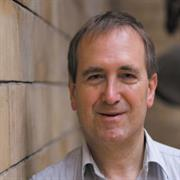
\includegraphics[width=.5\linewidth]{Stringer_Figure1}
	\caption{Professor Chris Stringer
	{\normalfont\scriptsize\\ \copyright\ by
                 % or NAME OF COPYRIGHT HOLDER
                  }}
	\label{fig:Stringer_Figure1}
\end{figure}
Professor Chris Stringer is currently a merit researcher at the Natural History Museum but also holds
an honorary professorship at University College London and is a visiting professor at Royal Holloway.
He is a fellow of the American Association for the Advancement of Science, Washington and the Royal Society as well as
being an Honorary fellow of the Society of Antiquities. 
He won the River’s Memorial Medal (2004) from the Royal Anthropological Institute and the Frink medal (2008) from
the Zoological Society of London. His early career was on the role of Neanderthals in hominin history,
leading to his role in the development of the Recent African Origin theory.
He now collaborates with a range of academics on projects intended to improve our understanding of hominin evolution.
Professor Stringer first studied Anthropology at University College London followed by a PhD at Bristol in Anatomical Science.
He has published papers in their hundreds and several books, one of the most recent being \emph{The Origin of Our Species},
published in the United States as \emph{Lone Survivors: How We Came to Be the Only Humans on Earth}.



\begin{labeling}{IJSRA}	
\item[IJSRA (International Journal of Student Research in Archaeology)] 
\emph{When and why did you become interested in physical anthropology?}
	
\item[Prof. Chris Stringer (CS)] 
My interest in human evolution started at primary school.
I was fascinated by fossils, and at the age of nine or ten did a school project on Neanderthals – I wish I still had it!
My interest grew through my school years but I had no idea that you could actually study in this area, so I planned to do medicine.
I had a place at medical school lined up, when I chanced upon University College London’s prospectus.
It was arranged alphabetically, and Anthropology was at the beginning.
The course offered archaeology, human evolution, genetics and social anthropology.
Suddenly medicine seemed much less appealing.
So I phoned UCL (this was long before the internet!), was invited for an interview, and offered a place.
Much to the amazement of my teachers and parents, I dropped medicine and took up this study subject,
which I had only just learnt existed.

\item[IJSRA] 
\emph{Do you think then that we need to publicise physical anthropology to younger audiences considering that you were
originally unaware that it was a subject area for study?}
	
\item[CS] 
Well I was from a working-class background in the East End of London, looking at the career choices offered by
teachers and the school library in 1966. Today, with online resources and social media,
I think both those giving advice and those looking for options have so much more information – maybe too much, at times!

\item[IJSRA]
\emph{Your publications range in topic from morphology, dating, climate, primatology, and isotopes.
Do you enjoy the interdisciplinary nature of your work? 
Is specialism and collaboration the future for archaeology and anthropology or is being a generalist a viable career choice?}

\item[CS]
I do enjoy the breadth, but it’s increasingly difficult to be a generalist in our area because of
the pace of new developments in highly specialised fields like DNA and isotopes.
I have to spend a lot of time trying to keep up with just the latest on DNA and the evidence for ancient hybridisation – that’s only one (big and ever-growing) area. Choosing the right collaborators is crucial!

\item[IJSRA]
\emph{You’ve run projects on hominins at an international (RESET project) and a national scale (Pathways to Ancient Britain).
Which types of project do you think are most informative for physical anthropology?}

\item[CS]
I’ve been lucky enough to be involved in a few finds of new material (e.g. Gough’s Cave) but
those large projects which seek to significantly increase the fossil record are, of course,
some of the most important – think what has emerged from sites like Liang Bua (\emph{floresiensis}) and Rising Star (\emph{naledi})
in the last few years. 
There are so many gaps in the geographical and chronological coverage, even in Africa, let alone vast areas of Asia or Oceania!
But for me, it’s also important to revisit old collections and apply new techniques of investigation – things like direct dating,
isotopes, taphonomic studies. 
We did that very successfully with AHOB (Ancient Human Occupation of Britain) and now with PAB,
and a whole new area of aDNA has also opened up now, of course.

\item[IJSRA]
\emph{Currently you are a leading academic on research into hominins and you are often quoted when new discoveries
have emerged (such as the recent discovery of \textup{Homo naledi}). When you first started your research however,
your support for the ‘Recent African Origin’ (RAO) hypothesis was in the minority as most supported the multi regionalism model.
Was it a relief when the RAO theory gained more support?}

\item[CS]
Well when I finished my PhD in 1974 I was pretty sure that modern humans had not evolved from European Neanderthals but
it took another decade before I was more certain that we had an African origin.
However this still-minority view was not really taken seriously until breakthroughs in DNA and dating in the late
1980s – then the polarisation and conflict really started to take off!

\item[IJSRA]
\emph{Recent research on hominin DNA and the discovery of hybridization, has led to some academics reverting back to
the multiregional model. 
Others suggest that now the human origins answer falls somewhere between the two.
What has been your experience in accepting (or rejecting) new research that usurps well established theory?}

\item[CS]
I’ve certainly learnt to expect the unexpected in the last few years!
I’d refer your readers to my book \emph{The Origin of our Species (Lone Survivors in the USA)} for more on how my views have changed,
and sometimes been forced to change!
Because we are human beings, and often very much in the public and media eye, it’s sometimes hard to
admit that we might have got it wrong, but as scientists it’s our duty to do so!
Presenting clear and testable ideas is a valuable service to science, but only if those ideas are at least credible in the first place.

\item[IJSRA]
\emph{With ancient DNA techniques, researchers have found both hybridization behaviour as well as
previously undiscovered hominins.
In your opinion, do you think this will lead to an assumption of a more diverse and bushy hominin phylogeny or
a more refined hominin family tree (lumping vs splitting classification)?}

\item[CS]
I think a bushy tree is already a reality but the species question applied to fossils is always going to be problematic.
I still think on morphology that the Neanderthals are specifically distinct from everyone alive today – they can be
distinguished just from their ear bones, for example.
But accepting that doesn’t mean accepting that they were reproductively isolated from us, as they clearly were not.
Closely-related mammal and bird species may take millions of years to become fully isolated from each other genetically.

\item[IJSRA]
\emph{You are currently affiliated with both the Natural History Museum and multiple Universities.
In your experience what are the main differences and advantages to working in these types of institutions?}

\item[CS]
I’ve got visiting/honorary professorships at two London Universities, so can make some comparisons.
A Museum can be a highly bureaucratic place at times, but it also has wonderful collections - and staff.
Having students around can be a great stimulus, but supervisions and assessments can take up a lot of time!
But I wouldn’t be where I am without some inspirational teaching and supervision along the way – and
I would take that comment right back to my primary schools!

\item[IJSRA]
\emph{As an academic who works in a museum, do you feel that current research reaches the general public?}

\item[CS]
I’ve always been aware of the need for outreach and have enjoyed contributing in the media and
giving talks to general audiences.
I do feel it is our responsibility to communicate beyond a purely academic audience, and I feel that an increasing number of
my colleagues share that view. 
Of course not everyone is a great communicator, but we can all try and do our bit!

\item[IJSRA]
\emph{Research on hominins generates a lot of media attention.
What are the benefits and draw backs of this interest and do you have a strategy for working with media outlets?}

\item[CS]
When there is a big story, it can take over your life for a few days if you let it,
and you always have to judge if it’s worth the time against the other things you were hoping to do!
Some stories are undoubtedly over-hyped or even completely misguided and I try to avoid engaging with those.
Our NHM press team is great at helping me manage the media storms which sometimes arise!

\item[IJSRA]
\emph{Our journal attempts to give a platform for archaeology students to publish in the early stages of their research.
Are open platforms and publications a valuable resource?}

\item[CS]
I do think open platforms and publications are valuable – my open access publication on \emph{Homo naledi} has
very quickly overtaken most of my other publications in terms of impact.
Undergrads need to get their formative ideas out there but they must also be prepared for the critiques
(some more measured and warranted than others) that almost always follow open access publication!

\item[IJSRA]
\emph{If you could go back to your undergraduate self, what piece of advice would you give?
Would you give this same advice to undergraduates now?}

\item[CS]
I think both then and now it’s to have a plan A and a plan B for your future.
I’ve been lucky enough that plan A has usually worked out, but putting all your eggs in one basket is not a good idea!
Also network as much as you can and try not to make enemies – you never know who you might need help from in the future!

\end{labeling}
\IJSRAclosing
\end{document}



%------------------------------
%\thispagestyle{empty}
\part{\scshape articles}

%------------------------------
\documentclass{ijsra}
\def\IJSRAidentifier{\currfilebase}
\def\shorttitle{Undergraduate Archaeological Skills Development in Western Autralia}
\def\maintitle{Testing a student driven, non-academic model for undergraduate archaeological skills development in Western Australia}
\def\shortauthor{Jane Fyfe, Sean Winter, Ashleigh Murszewski}
\def\authormail{jane.fyfe@graduate.uwa.edu.au}
%\def\affiliation{1Archaeology M257, University of Western Australia, 35 Stirling Highway, Crawley, Western Australia 6009}
%\def\affiliation{2Australian Archaeomagnetism Laboratory, Department of Archaeology, Faculty of Humanities and Social Sciences, La Trobe University, Melbourne Campus, Bundoora, VIC 3086, Australia}
\def\thanknote{Jane Fyfe is currently completing a PhD in archaeology at the University of Western Australia, and working in Aboriginal Health Training. She has many research interests, including the intersection of historical and Indigenous archaeologies, the role of rock art in all its forms (from prehistoric pigment and engravings to contemporary graffiti) in identity formation and resistance. Jane is also interested in exploring the stories and archaeologies of the unseen and unheard through historical and contemporary archaeology. She is passionate about teaching and sharing archaeology with university students, community volunteers and enthusiasts, especially its practical application and interpretation. She has published in journals her work on historical inscriptions in the Torres Strait and rock art in northern Australia, as well as her PhD research in the southern Kimberley, Western Australia and presented her research at Conferences in the USA and Australia.
	
Sean Winter is an early career researcher currently working in Western Australia. He has diverse research interests with a primary concentration on historical archaeology in Australia. He also has secondary interests in the archaeology of the Greco-Roman period in Egypt; in the archaeology of World War II; in methodological issues related to excavation and stratigraphy, particularly related to urban sites and buildings archaeology; in issues related to teaching and learning in archaeology; and in heritage issues related to convict sites. He has published in numerous journals and will shortly be releasing a book on the convict system in Western Australia.

Ashleigh Murszewski is a developing geoarchaeologist working on various deposits within Western Australia and Southern Africa. With a dual qualification in geology and archaeology, she has pursued an interdisciplinary specialty focusing on understanding geomorphological context of archaeological and palaeoanthropological sites. Current research projects include; local sedimentology of alluvial and karst sequences (inc. micromorphological and sedimentological applications) and, regional studies of palaeocave formation and survival. She has published and presented in Australian journals and conferences on her research in Western Australia, and will commence a PhD at La Trobe University, Melbourne, Victoria in 2016.}
\def\keywords{Community, pedagogy, students, skills development, ethics, research}
%\def\keywordname{}
\begin{filecontents}{\IJSRAidentifier.bib}
@ARTICLE {aitchison2004,
author  = "Ken Aitchison",
title   = "Supply, demand and a failure of understanding: addressing the culture clash between archaeologists' expectations for training and employment in 'academia' versus 'practice'",
journaltitle = "World Archaeology",
year    = "2004",
volume  = "36",
number  = "2",
pages   = "203--219"
}


@MANUAL {AAA2004,
title  = "Code of Ethics",
author = "Australian Archaeological Association Inc.",
year   = "2004"
}


@MANUAL {aacai,
title        = "Code of Ethics",
author       = "AACAI",
organization = "Australian Association of Consulting Archaeologists",
}


@BOOK {beck2008,
editor    = "Beck, W.",
title     = "By Degrees. Benchmarking archaeology degrees in Australian Universities",
publisher = "Teaching and Learning Centre, University of New England",
year      = "2008",
location   = "Armidale, NSW"
}


@ARTICLE {beck2005,
author  = "Beck, W. and Balme, J.",
title   = "Benchmarking for archaeology honours degrees in Australian Universities",
journaltitle = "Australian Archaeology",
year    = "2005",
volume  = "61",
pages   = "32--40"
}


@INPROCEEDINGS {bowdler1984,
author       = "Bowdler, S.",
title        = "Archaeological significance as a mutable quality",
booktitle    = "Site Surveys and Significance Assessment in Australian Archaeology: Proceedings of the 1981 Springwood Conference on Australian Prehistory",
year         = "1984",
editor       = "Sullivan, S. and Sandra Bowdler, S.",
pages        = "1--9",
location      = "Canberra",
organization = "Australian National University",
publisher    = "Department of Prehistory, Research School of Pacific Studies"
}


@INCOLLECTION {boytner2012,
author    = "Boytner, R.",
title     = "The UCLA Archaeology Field Schools Program: Global Reach, Local Focus",
booktitle = "Global Perspectives on Archaeological Field Schools. Constructions of Knowledge and Experience",
publisher = "Springer",
year      = "2012",
editor    = "Mytum, H.",
pages     = "83--102",
location   = "New York"
}


@ARTICLE {brown2008,
author  = "Brown, S.",
title   = "Mute or Mutable? Archaeological Significance, Research and Cultural Heritage Management in Australia",
journaltitle = "Australian Archaeology",
year    = "2008",
volume  = "67",
pages   = "19--30"
}


@BOOK {burke2004,
author    = "Burke, H. and Smith, C.",
title     = "The Archaeologist's Field Handbook",
publisher = "Allen and Unwin",
year      = "2004",
location   = "Crowís Nest"
}


@MISC {busher2012,
author = "Busher, N.",
title  = "Site formation processes on a river floodplain: a case study from West Toodyay, Western Australia",
year   = "2012",
note   = "Poster presented at Joint Australasian Society for Historical Archaeology and Australasian Institute for Maritime Archaeology Conference, Fremantle, Australia, October 2"
}


@INCOLLECTION {clark2012,
author    = "Clark, Bonnie J.",
title     = "From Graduate to Professor: Changing Perspectives on Field Schools",
booktitle = "Global Perspectives on Archaeological Field Schools. Constructions of Knowledge and Experience",
publisher = "Springer",
year      = "2012",
editor    = "Mytum, H.",
pages     = "217--228",
location   = "New York"
}


@INCOLLECTION {cobb2012,
author    = "Cobb, H. and Croucher, K.",
title     = "Field Schools, Transferable Skills and Enhancing Employability",
booktitle = "Global Perspectives on Archaeological Field Schools. Constructions of Knowledge and Experience",
publisher = "Springer",
year      = "2012",
editor    = "Mytum, H.",
pages     = "25--40",
location   = "New York"
}


@ARTICLE {colley2004,
author  = "Colley, S.",
title   = "University-based Archaeology Teaching and Learning and Professionalism in Australia",
journaltitle = "World Archaeology",
year    = "2004",
volume  = "36",
pages   = "189--202"
}


@ARTICLE {colley2007,
author  = "Colley, S.",
title   = "Public Benefits of Archaeology: Results from a Student Questionnaire",
journaltitle = "Australian Archaeology",
year    = "2007",
volume  = "65",
pages   = "30--36"
}


@INCOLLECTION {colley2012,
author    = "Colley, S.",
title     = "Archaeological Field Schools and Fieldwork Practice in an Australian Context",
booktitle = "Global Perspectives on Archaeological Field Schools. Constructions of Knowledge and Experience",
publisher = "Springer",
year      = "2012",
editor    = "Mytum, H.",
pages     = "61--82",
location   = "New York"
}


@ARTICLE {cosgrove2013,
author  = "Cosgrove, R. and Frankel, D. and Thomas, D.",
title   = "From the moat to the Murray: Teaching practical archaeology at La Trobe University, Australia",
journaltitle = "Australian Archaeology",
year    = "2013",
volume  = "76",
pages   = "44--51"
}


@ARTICLE {faulkner2000,
author  = "Faulkner, N.",
title   = "Archaeology From Below",
journaltitle = "Public Archaeology",
year    = "2000",
volume  = "1",
pages   = "22--33"
}


@ARTICLE {fredericksen2005,
author  = "Fredericksen, C.",
title   = "Archaeology out of the classroom: Some observations on the Fannie Bay Gaol field school, Darwin.",
journaltitle = "Australian Archaeology",
year    = "2005",
volume  = "61",
pages   = "41--47"
}


@ARTICLE {gibbs2005,
author  = "Gibbs, M. and Roe, D. and Gojak, D.",
title   = "Useless graduates? Why do we all think that something has gone wrong with Australian archaeological training?",
journaltitle = "Australian Archaeology",
year    = "2005",
volume  = "61",
pages   = "24--31"
}


@ARTICLE {hall2005,
author  = "Hall, J. and O'Connor S. and Pragnell, J. and Smith, T.",
title   = "Teaching archaeological excavation at the University of Queensland: Eight years inside TARDIS",
journaltitle = "Australian Archaeology",
year    = "2005",
volume  = "61",
pages   = "48--55"
}


@ARTICLE {ireland2013,
author  = "Ireland, T. and Guthrie, A. and Mackay, R. and Smith, A.",
title   = "Historical archaeology and Australia`s cultural heritage sector:emerging issues for education and skills development",
journaltitle = "Australasian Historical Archaeology",
year    = "2013",
volume  = "31",
pages   = "3--13",
}


@MISC {murszewski2012,
author = "Murszewski, A.",
title  = "Student training and meaningful projects: developing an appropriate research framework for Statham's Quarry",
year   = "2012",
date   = "2012-10-02",
location = "Fremantle, Australia",
eventtitle = "Joint Australasian Society for Historical Archaeology and Australasian Institute for Maritime Archaeology Conference",
}


@MISC {murszewskiwinter2012,
author       = "Murszewski, A. and Winter, S.",
title        = "A Preliminary Report of Archaeological Investigation at Stathamís Quarry, Gooseberry Hill, Western Australia",
howpublished = "Unpublished report for the Archaeological Society of Western Australia",
year         = "2012"
}


@INCOLLECTION {mytum2012a,
author    = "Mytum, H.",
title     = "The Pedagogic Value of Field Schools: Some Frameworks.",
booktitle = "Global Perspectives on Archaeological Field Schools. Constructions of Knowledge and Experience",
publisher = "Springer",
year      = "2012",
editor    = "Mytum, H.",
pages     = "9--24",
location   = "New York"
}


@INCOLLECTION {mytum2012b,
author    = "Mytum, H.",
title     = "Two-Centre Field Schools: Combining Survey and Excavation in Ireland and Wales or the Isle of Man",
booktitle = "Global Perspectives on Archaeological Field Schools. Constructions of Knowledge and Experience",
publisher = "Springer",
year      = "2012",
editor    = "Mytum, H.",
pages     = "103--118",
location   = "New York"
}


@INCOLLECTION {mytum2012c,
author    = "Mytum, H.",
title     = "Introduction",
booktitle = "Global Perspectives on Archaeological Field Schools. Constructions of Knowledge and Experience",
publisher = "Springer",
year      = "2012c",
editor    = "Mytum, H.",
pages     = "3--8",
location   = "New York"
}


@INCOLLECTION {pyburn2003,
author    = "Pyburn, K. A.",
title     = "What are we really teaching in Archaeological Field Schools?",
booktitle = "Ethical Issues in Archaeology",
publisher = "Altamira Press",
year      = "2003",
editor    = "Zimmerman, L. and Vitelli, K. and Hollowell-Zimmer, J.",
pages     = "213--224",
location   = "Walnut Creek"
}


@BOOK {renfrew2000,
author    = "Renfrew, C. and Bahn, P.",
title     = "Archaeology: Theories, Methods and Practice",
publisher = "Thames \& Hudson",
year      = "2000",
location   = "London",
edition   = "3"
}

@INCOLLECTION {scarlett2012,
author    = "Scarlett, T. J. and Sweitz, S. R.",
title     = "Constructing New Knowledge in Industrial Archaeology.",
booktitle = "Global Perspectives on Archaeological Field Schools. Constructions of Knowledge and Experience",
publisher = "Springer",
year      = "2012",
editor    = "Mytum, H.",
pages     = "119--146",
location   = "New York"
}


@MANUAL {saa1996,
title        = "Principles of Archaeological Ethics",
author       = "SAA",
organization = "Society for American Archaeology",
year         = "1996"
}


@ARTICLE {ulm2013,
author  = "Ulm, S. and Mate, G. and Dalley, C. and Nichols, S.",
title   = "A working profile: The changing face of professional archaeology in Australia",
journaltitle = "Australian Archaeology",
year    = "2013",
volume  = "76",
pages   = "34--43"
}


@ARTICLE {ulm2005,
author  = "Ulm, S. and Nichols, S. and Dalley, C.",
title   = "Mapping the shape of contemporary Australian archeology: implications for archaeology teaching and learning",
journaltitle = "Australian Archaeology",
year    = "2005",
volume  = "61",
pages   = "11--23"
}


@MANUAL {wac1990,
title        = "First Code of Ethics",
author       = "WAC",
organization = "World Archaeological Congress",
year         = "1990"
}
\end{filecontents}

\begin{document}
\IJSRAopening
	{\Large\scshape
	%\shortauthor
    Jane Fyfe\textsuperscript{$\dagger$}, %
    Sean Winter\textsuperscript{$\dagger$}, %
    Ashleigh Murszewski\textsuperscript{$\dagger\ddagger$}%
    }%
	\footnote\thanknote%
	\\[1em]
	\email\\
    {\textsuperscript{$\dagger$}University of Western Australia\\
     \textsuperscript{$\ddagger$}La Trobe University, Melbourne}
	%\affiliation
\IJSRAmid

\begin{IJSRAabstract}
Australia\marginnote{Abstract} is not unique in identifying the gap between the skillset required to work in the archaeology profession and the skills provided during a standard archaeology degree. 
The most significant and enduring gap has been identified by the students themselves; the practical application of archaeological field skills. 
In Western Australia, students have taken the initiative, and moved away from the academic world, to develop a practical model for supervised, structured fieldwork that increases practice opportunities and, consequently, their skills and confidence in this area when they graduate.
A model for skills development, designed and tested by the Archaeological Society of Western Australia, demonstrates that using a flexible approach within a well-structured model may be used effectively for a variety of projects, whilst meeting both the ethical and legal needs contiguous in archaeological practice. 
This non-academic model offers real research and field experiences to students, to enhance their skill development and complement their academic studies. 
The model’s flexibility provides the capacity for implementation both within and outside of Australia.

\end{IJSRAabstract}

\section{Introduction}

\lettrine[nindent=0em,lines=3]{A}{rchaeological} fieldwork may take many forms and future archaeologists need relevant training in a range of skills, including, but not limited to, excavation, survey, building recording, artefact analysis, and the many aspects of teamwork and organisation associated with fieldwork. 
Developing a range of skills to an appropriate level of competency takes time and effort, both on the part of students and those teaching them. Over the past decade there has been an ongoing discussion within the discipline of archaeology in Australia regarding the level of practical skills gained during a standard three or four-year archaeology degree. 
The debate over whether universities provide sufficient practical training to appropriately prepare undergraduates for the realities of the profession has at times become heated \parencites[e.g.][]{cobb2012}{mytum2012a}{ulm2005}{ulm2013}. 
Profiles of the discipline in Australia suggest that commercial and consulting practitioners see a disparity between practical skills taught at universities \parencite{beck2005}{colley2012}{cosgrove2012}{fredrickson2005}{hall2005}
 and the needs of professional practice \parencite{colley2004}{colley2012}{cosgrove2013}{gibbs2005}{ireland2013}{ulm2005}{ulm2013}. 
 This issue is not restricted to Australia; it has also been the subject of research and discussion in over the last decade in Britain \parencites [e.g.][]{aitchison2004}{cobb2012} and the USA
  \parencite[e.g.][]{boytner2012}.

Archaeological professionals are not the only group concerned about the development of appropriate skills; many students are also aware of the need to develop and, crucially, to apply practical skills that will prepare them for employment as professional archaeologists. 
This paper describes a student initiated and driven attempt to acquire skills development and field experience outside of the standard university curriculum, but within the limited finances of most students. 
It represents a rare example of a fieldwork training program driven by students rather than academics. 
In addition, the students involved identified the opportunity to provide public benefit through real projects in the heritage sector, with students directly involved in framing the research questions and selecting and managing projects that would also meet their skills development needs.

The issues and case studies in this paper relate specifically to Western Australian conditions and legislative limitations, however, the experiences of others \parencites[e.g.][]{boytner2012}{mytum2012a}{mytum2012b}{scarlett2012} suggest that this example has application beyond Western Australia.
Surveys conducted as part of an ongoing research project into volunteering in archaeology in Australia suggest that the majority of people who take-up volunteer archaeological opportunities are students seeking to develop skills (Winter 2014 pers. Comm.).%HOW TO CITE THIS
This research also suggests that those opportunities are usually short term, occasional and sporadic. 
The research, fieldwork and reporting processes in this approach are run by undergraduate students, who are able to drive fieldwork themselves, in their own time frames, rather than being dependent on inclusion in ad-hoc opportunities provided by academic and commercial archaeology research projects \parencites[see][90]{boytner2012}[222]{clark2012}[70-72]{colley2012}. 

\section{Background}

There is no set standard of qualifications to work in archaeology in Australia, however, it is suggested that students complete a minimum of a three-year bachelor degree, with the addition of an honours year or a postgraduate diploma, to become a registered professional able to report to government. 
This varies from state to state; some states have regulations specifying required qualifications, whereas Western Australia does not. 
The degree typically includes field and laboratory tuition, although the extent of this varies \parencite{gibbs2005}. 
Universities are risk averse \parencite[6]{boytner2012}, and fieldwork is costly and time consuming for small academic departments. 
Archaeology is often part of a liberal arts degree, where limited staff and funding does not provide for fieldwork or the laboratories and tuition needed in the discipline \parencites{colley2004}{colley2012}{gibbs2005}{cosgrove2013}. 
Archaeology courses at Australian universities appeal to a wide audience, and many students study a selection of archaeology subjects as part of broader liberal arts and science degrees, with no intention of working in the profession \parencites[28]{gibbs2005}[44]{cosgrove2013}; 
though that may change with exposure to fieldwork opportunities \parencite[29]{cobb2012}. 
The \textcite[31]{cobb2012} study suggested that in the UK as few as 15\% of students who start an archaeology degree finish their degree working in the profession. 
Universities may justifiably argue that providing expensive, time-consuming courses that concentrate on developing a skill set for the use of a small number of students is not an essential part of an archaeology degree.

Beyond this is the ethical issue of whether it is appropriate to have students engaged in the archaeological excavation of sites, when they do not have the skills or experience to do so appropriately. 
As excavation is destruction, numerous commentators have questioned whether the presence of students can do more harm than good \parencites[48]{hall2005}[216]{pyburn2003}. 
This becomes a circular argument, in that students cannot gain appropriate experience to contribute effectively if there are no opportunities to participate in fieldwork. 
The argument then devolves to the most ethically sound way to include students in fieldwork opportunities without risking the integrity of archaeological sites, with options such as the inclusion of small numbers of students in larger research projects, appropriately taught field schools on real sites \parencite{mytum2012c}, 
and the creation of “fake” excavation resources \parencites{cosgrove2013}{hall2005}. 
There is also the ethical requirement that fieldwork operates and is driven by appropriate research questions. Some students see fieldwork not as a process to answer research questions, but as the end goal of archaeology itself. 
This makes it essential to embed fieldwork opportunities for students within suitable research driven projects.

Standards for practical archaeological skills taught in Australian universities are set out in the document \emph{By Degrees: Benchmarking archaeology degrees in Australian Universities} 
\parencite{beck2008}, which provides a list of competencies for standard archaeology degrees. While there is no requirement or guidance for implementation, the report states explicitly that, 
"\emph{To ensure continued effective learning, adequate funding is required to design and run field schools and laboratory practicals of the highest national and international standards}" \parencite[9]{beck2008}.

University degrees available in Australia offer a range of options for field and laboratory practical opportunities, and each university with an archaeology major has a different model for teaching practical skills.
However, within a standard archaeology major, options for developing practical skills may lie in as few as one or two field schools, a general laboratory unit, and occasional practical options within other courses of study. 
The non-compulsory nature of these units within a larger archaeology degree means that students can, and often do, graduate with an archaeology degree in which they have had no real exposure to any form of field or laboratory training.

There are other issues with university field training; students tend to learn one way of doing things relevant to the site on which they are working, without experiencing the wide range of techniques that are applicable in differing situations. 
For example, single context excavation and recording at an urban historical site requires a different approach to excavation than test pitting at an Indigenous rock-shelter site. 
Additionally, as suggested by \textcite[44]{cosgrove2013}, in our own undergraduate and teaching experiences and 
those reported in recent surveys (Winter \& Beale 2014 pers. Comm.) university training is usually very much of the moment and students rarely see either the research and preparation undertaken prior to excavation or the end product of their fieldwork, which generally includes the production of reports or analysis of artefact assemblages.

Practical archaeological skills are demanding, requiring high levels of proficiency and confidence in their practical application and decision making and organisation that take time to develop. 
When compared to a standard trade apprenticeship - where an apprentice is expected to do three or four years full time of practical work along with formal classroom training, before being considered qualified - archaeological skills training available in an undergraduate archaeology degree appears limited. 
Nevertheless, the Consulting Archaeology industry, in which most graduates in Australia are likely to gain employment, continues to expect students to graduate with a higher skill level than provided within a standard degree \parencites{colley2004}{colley2012}{gibbs2005}. 
Universities work effectively to teach practical skills within considerable economic and temporal constraints. However, in the current fiscal environment universities are also severely limited in their capacity to provide greater field opportunities for students to develop the desired skill sets.

Students aiming for a career in archaeology are encouraged to be proactive, and seek fieldwork complementary to their studies to aid skill development. 
Avenues for this are often limited by factors such as geography, cost and time or timing. 
For example, current research into volunteering in Australian archaeology suggests that the majority of volunteer projects are short term, with limited avenues for ongoing practical volunteering (Winter 2014 pers. Comm.). 
Other options include participation in occasional post-graduate fieldwork projects, or paying inflated prices to attend overseas field schools, or those run by specialists at other Australian universities. 
Competition is often fierce for local volunteer roles and many projects cannot accommodate, or afford to supervise, the large numbers of students seeking to develop field skills, particularly when the project also has a commercial aspect. 
In response to this need, the \emph{Archaeological Society of Western Australia} (ASWA), a volunteer body of mostly archaeology undergraduates, began a discussion to identify regular ongoing opportunities that would assist their members to develop and practice their skills outside the academic environment. 

Over a number of years, ASWA has been involved in projects in which it was often confronted with the problem that the students who run the society were not qualified to teach other students, nor did they have the skills or experience to develop or manage appropriate archaeological projects. 
Qualified and experienced archaeologists were needed to assist. This meant that fieldwork opportunities for ASWA members were ad-hoc, and linked to fieldwork carried out by postgraduate students within the group. 
To reduce this shortcoming and increase opportunities, ASWA sought to develop an ongoing process using a public archaeology framework (i.e. driven by the community \parencite {faulkner2000}) with an ongoing field project that would both provide learning and practice opportunities, and develop links between the archaeological profession and members. 
The premise was to include more professionals in Society activities, thus providing greater fieldwork opportunities in the future. 
ASWA would initiate and manage each project, and develop links with professionals to join the project to supervise students and develop their skills. 
In other words, the students develop and drive their own projects and tap into professional knowledge to enable them to do this.

Implicit in this overarching aim is the concept that any field project should help students develop discipline specific field skills, and be based on real archaeological sites and driven by real research questions, rather than at manufactured or re-created excavation sites used by some Australian universities for teaching field skills \parencites[e.g.]{cosgrove2013}{hall2005}. 
This does not question the efficacy of such schemes, but members were explicit in their desire to work on real sites. 
ASWA also needed fieldwork opportunities that would not be prohibitively expensive to participate in, an issue with many archaeological field schools, both domestic and international. 
Finally, the project would be ongoing, and involve a number of professional archaeologists, to remove ASWA’s reliance on postgraduate students for fieldwork opportunities.

In developing the model flexibility was essential. This included being able to conduct research around available and local opportunities as well as identifying projects and professional archaeological expertise that would cater for relatively large groups (up to 30 at a time, reflecting the large membership of ASWA). 
The skills developed in the projects needed to be useful and appropriate to future archaeological careers; provide for the ongoing application of those skills in real archaeological research activities, and, in keeping with ASWA’s overarching community based approach, the projects and their outcomes would need to have an identifiable benefit to the wider Western Australian community.

\section{Developing the Model}

A project committee, comprising the Executive of ASWA and two qualified archaeologists, current postgraduate members, convened to create a model to support the identification and development of archaeological fieldwork that would meet the identified needs. 
From the beginning, the committee agreed that this was not to replicate or replace university fieldwork training, but to complement it and provide additional opportunities for the application of knowledge and skills already acquired at university.

Ethical issues and community perceptions were important considerations in developing a model that would allow students to work on real sites with genuine outcomes. As such, the model needed to include:

\begin{enumerate}
	\item non-destructive fieldwork processes;
	\item compliance with legislative and regulatory requirements enshrined in Western Australian heritage law;
	\item consultation and/or negotiation with appropriate stakeholders; and
	\item research questions.
\end{enumerate}

The necessity for non-destructive fieldwork processes meant the project prioritised skills based around survey and recording of existing archaeological features, crucial skills for any archaeologist. 
Furthermore, the model would involve students in the full range of project design and completion; including site identification, planning, background research, logistics, recording and reporting. 
As such, fieldwork was only one part of the model. The model design reflects many of the same range of skills identified as desirable by \textcite[40-41]{ulm2013} in a survey of professional archaeologists in Australia. 
Field survey, report writing, research and leadership skills ranked in the top ten most valuable skills \parencite[40]{ulm2013}, 
with report writing and site survey identified as two of the most used skills in the heritage sector \parencite[10]{ireland2013}. 
Time and financial limits of students, and ensuring the involvement of professional archaeologists in leading teams, resulted in a model designed specifically for use in regular individual fieldwork days rather than over extended field seasons.

The next stage was identifying suitable sites. The Committee agreed that using sites perceived to be of low significance and publicly accessible would be suitable for projects that would both benefit the students seeking skills development, and provide a contribution to the public record (Community benefit). 
The main aims of the model were finalised (\cref{fig:Fyfe-Table01}) and the potential achievable outcomes identified (\cref{fig:Fyfe-Table02}) through this iterative process of discussion and consultation with members.

   	\begin{figure} %TABLE 1
   		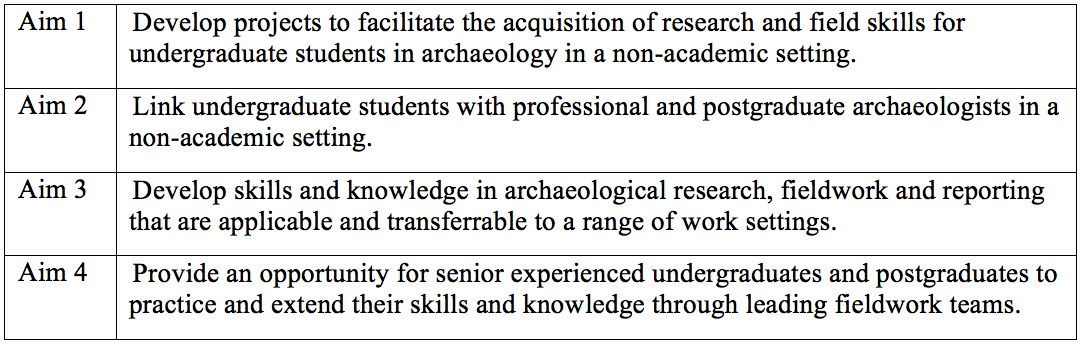
\includegraphics[width=\linewidth]{figures/Fyfe-Table01}
   		\captionof{table}{Aims of the non-academic skills development model.}
   		\centering
   		\label{fig:Fyfe-Table01}
   	\end{figure}	

   	\begin{figure} %TABLE 2
   		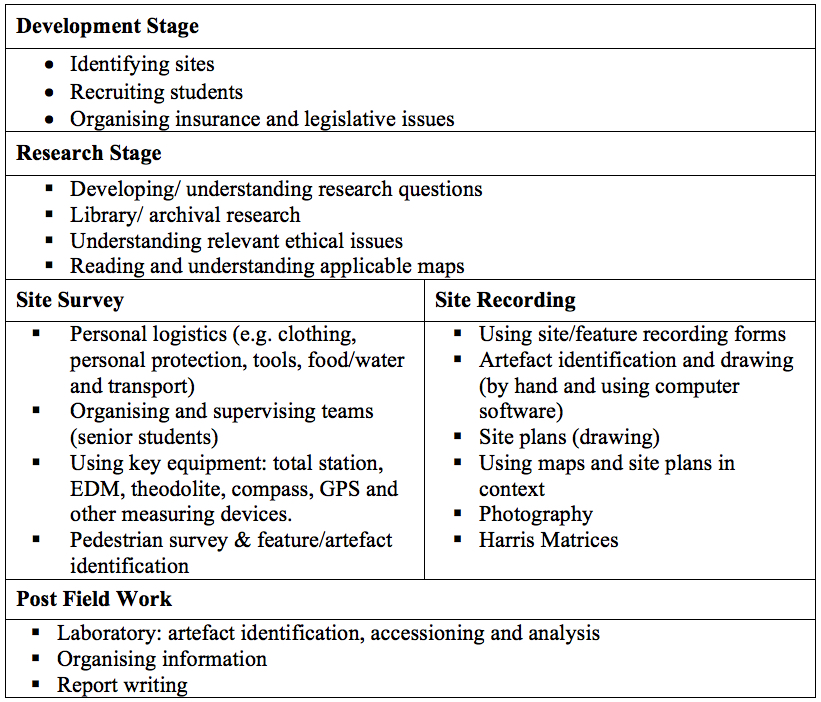
\includegraphics[width=\linewidth]{figures/Fyfe-Table02}
   		\captionof{table}{Aims of the non-academic skills development model.}
   		\centering
   		\label{fig:Fyfe-Table02}
   	\end{figure}

In addition, a template was created to give students a clear framework for planning and organising the research, gathering data and reporting it in an appropriate format. 
The final report format forms an important component of the archaeological record for sites for which little information is available, and contributes to the heritage of Western Australia in keeping with professional standards (e.g. \emph{Australian Archaeological Association, Australian Association of Consulting Archaeologists, World Archaeological Congress, and Society of American Archaeology Codes of Ethics}). 
The recording and reporting gives students a tangible outcome from the fieldwork, which \textcite[113-116]{mytum2012c} concludes is an important element of effective learning.

The first two stages allow for small groups, or individuals, to undertake desktop and archival research in preparation for the fieldwork component of the project. 
This develops and enhances research skills, implicit and explicit in project aims one and three. Similarly, maps accessed for the report, the results of background research and liaison with professional archaeologists, historians, librarians and others links to project aims one to three. 
The other stages allow for the incorporation of the data gathered in the field, including drawings and measurements, and relate well to the application of skills in aim three.

The model, with the identified skills and the reporting template, have been designed to meet the needs that students themselves identified, and to complement the skills developed through university courses in Australia \parencite[3]{beck2008}. 
The most likely employment for Australian graduates is to work in an archaeological consultancy, and the skill sets developed will be relevant to future careers in this area \parencites[e.g.][]{ireland2013}{ulm2005}{ulm2013}. 
There is also a degree of crossover with the academic side of the profession, where a similar set of research, technical and operational skills are important constituents of academic research.

\section{Case Study One: Canning Mills}

The first site for fieldwork was at Canning Mills, located on the outskirts of the Perth metropolitan area, approximately \SI {30}{\kilo\meter} 
to the south east of the city centre (\cref{fig:Fyfe-Figure01}). 
The site is an abandoned timber mill with an adjacent residential area, in use between c.1890 and 1930. 
Much of the land was rehabilitated, and has returned to forest, but a number of features are still visible. The site is not registered or protected under any legislative or regulatory provisions; it is in a semi-remote location on public land, and there is rapid degradation from large scale rubbish dumping and bushfires. A number of archaeological features (including structural foundations) are extant and, with easy access from the city, it was an ideal location to test the model.

   	\begin{figure} %FIGURE 1
   		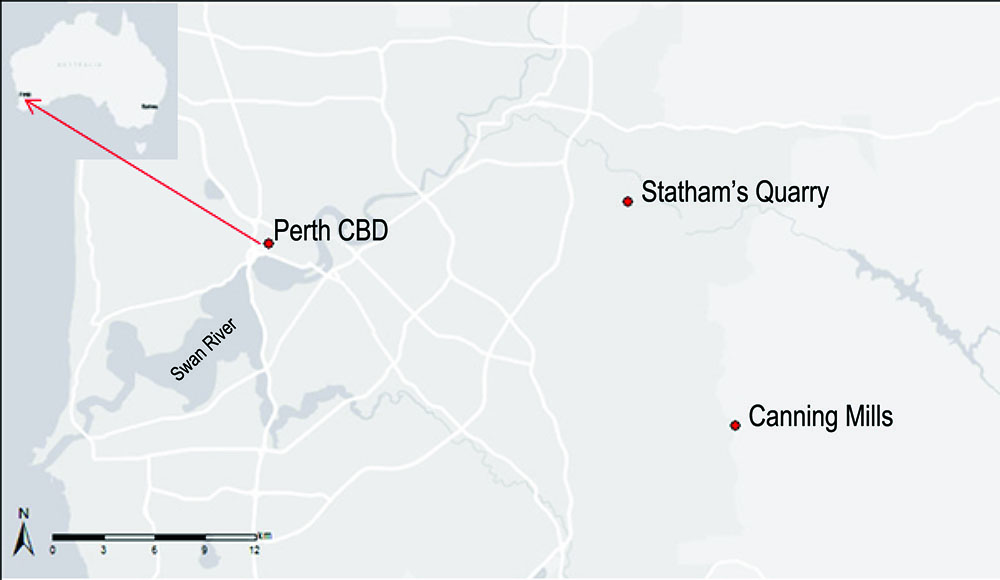
\includegraphics[width=\linewidth]{figures/Fyfe-Figure01}
   		\caption{Map showing the location of the sites referred to in this study, Canning Mills and Statham’s Quarry.}
   		\centering
   		\label{fig:Fyfe-Figure01}
   	\end{figure}

ASWA used social media, lecture announcements and emails to alert students to this fieldwork opportunity, and provided public liability insurance cover for the member volunteers. 
Demand from members was so high that a cap was set on the numbers able to participate. 
This meant there were enough students and supervisors sufficient to form five teams, each of which would undertake specific aspects of site recording.

Fieldwork processes and the skills to be developed were framed around an appropriate research question, following the initial site inspection. A self-selected group undertook archival and library research, identifying and accessing maps and documents relevant to planning the fieldwork.
Fieldwork logistics were the responsibility of fieldwork leaders, and all participants were responsible for their own personal protective equipment and field equipment, including field books, food and water.

Professional archaeologists including PhD candidates, consultants and museum staff led fieldwork. 
The field day began with an occupational health and safety briefing, site background, team allocations and responsibilities. Two teams conducted pedestrian surveys. One survey used \SI{5}{\meter} transects of the revegetated bushland to identify and record surface scatters of artefacts and a fenced grave. 
One team surveyed the edge of the road bordering the site, locating and recording the remains of a rail line used for timber transport while another team recorded and photographed surface scatters of glass, ceramics and metal remains across the open area of the site to the south of the roadway. 
Background research and maps of the site suggested that there had been a cricket pitch with buildings to the south east, and a team searched in dense bush for remains of these structures, however failed to find any evidence, an important experience for the students. 
Finally, the fifth team drew a plan of the remains of a large house with an extant curved stairway at the entrance and substantial remains of the foundations.

During the field day students were involved in site survey, feature identification, artefact identification and drawing, photography, site drawing, using GPS to record and locate features, map reading, data recording and team work. 
Communication was an essential skill at this large, densely forested site where only two of the teams were within visual range of one another; team leaders and the site director ensured that each team was well-briefed and contactable, an important precaution and planning skill for archaeologists in Australia who often work in isolated areas. 
In addition, some senior students had an opportunity to lead teams, make interpretations and decisions in the field, to guide less experienced students.

\section{Evaluating the Process}

Feedback from participants on the field day was excellent, with most students indicating that they relished the opportunity to practice skills they had learnt, or been introduced to, at university. 
The documentation produced by the students also showed that it had been an effective learning experience, with usable data, plans, and a range of drawings and photographs documenting the site. 
Writing of the post-field report was problematic. Students self-selected to write the report, but with the return to university life, including assessments and exams, the report writing lingered and was gradually abandoned. It was eventually completed by one of the postgraduate supervisors with little input from other members post field day.

The evaluation was that preparation for fieldwork and participation may generate enthusiasm and excellent results in terms of skill development and application. 
A lack of supervision and/or personal incentive after the field day led to a waning of that passion, and the result was that analysis and reporting skills important to future archaeological work were not practiced.

The model was revised to include a different post-fieldwork reporting process. While a report may be the preferable outcome, any output that forms an accessible, permanent record of archaeological work at the site is acceptable. 
The revised model also allocated the reporting phase to a single student, mentored by a professional archaeologist, which meant that the report process was manageable and provided that student with an outcome that could be listed on their CV. 
In addition, this second version of the model allowed for a range of alternative measurable outcomes, such as posters, conference presentations or reflective essays, dependent upon the needs of the project and to the benefit of the particular student. 
This meant that individuals could use the project to contribute to their wider skills resume, improving motivation as well as knowledge and skills for employment (\cref{fig:Fyfe-Figure02}). This was also designed to be more flexible to respond to the differences in sites, the needs of individuals and to provide a range of measurable outcomes.

   	\begin{figure} %FIGURE 2
   		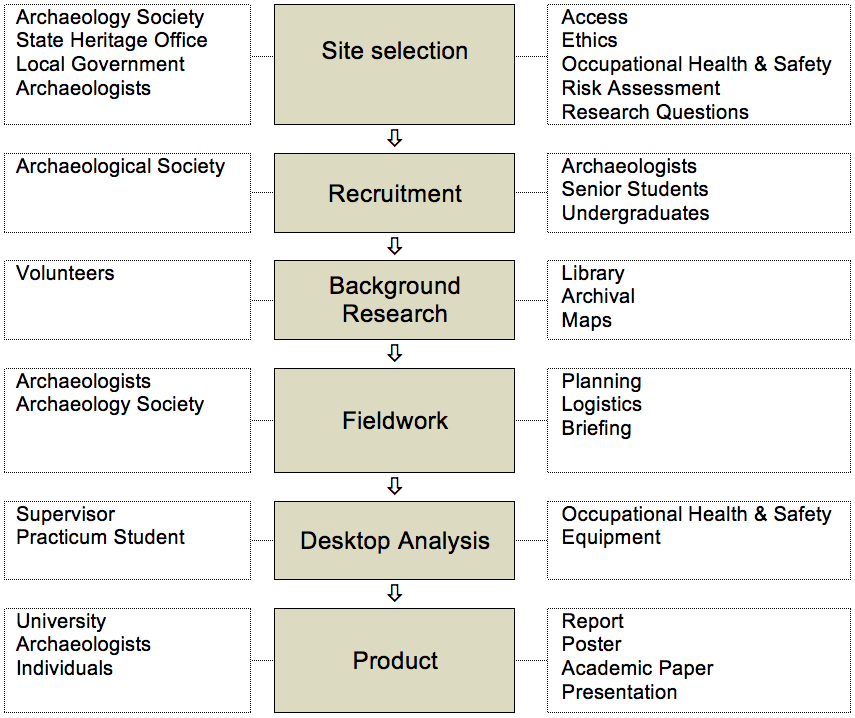
\includegraphics[width=\linewidth]{figures/Fyfe-Figure02}
   		\caption{Revised skills development model.}
   		\centering
   		\label{fig:Fyfe-Figure02}
   	\end{figure}

\section{Case Study Two: Statham's Quarry}

The revised model was used at Statham’s Quarry, a late 19th to early 20th century industrial complex located in the Darling Range east of Perth, Western Australia (\cref{fig:Fyfe-Figure01}). Unlike Canning Mills this site is listed on the State Heritage Register. It is located in Gooseberry Hill National Park and is a popular location for bushwalkers, rock climbers and a range of other recreational activities; therefore, access was not an issue.

Once again, there was high demand for this field day, and the 30 available positions filled within a few days. A team of five students conducted the archival research for the site before the field day, and 28 students, and four archaeologists, including one from the State Heritage Office, undertook the fieldwork. 
In a single day of survey, 46 archaeological features were recorded. 
Students gained valuable experience in research and site survey methodology (see \cref{fig:Fyfe-Figure03}), successfully gathering information on the layout and operation of the quarry, and associated industrial and residential buildings. 
The size of Statham’s Quarry allowed students to be involved in assessing multiple features at the site and to record them accurately under supervision. Therefore, students applied their skills using a variety of archaeological tools and methods likely to be utilised by companies in the professional sphere.

   	\begin{figure} %FIGURE 3
   		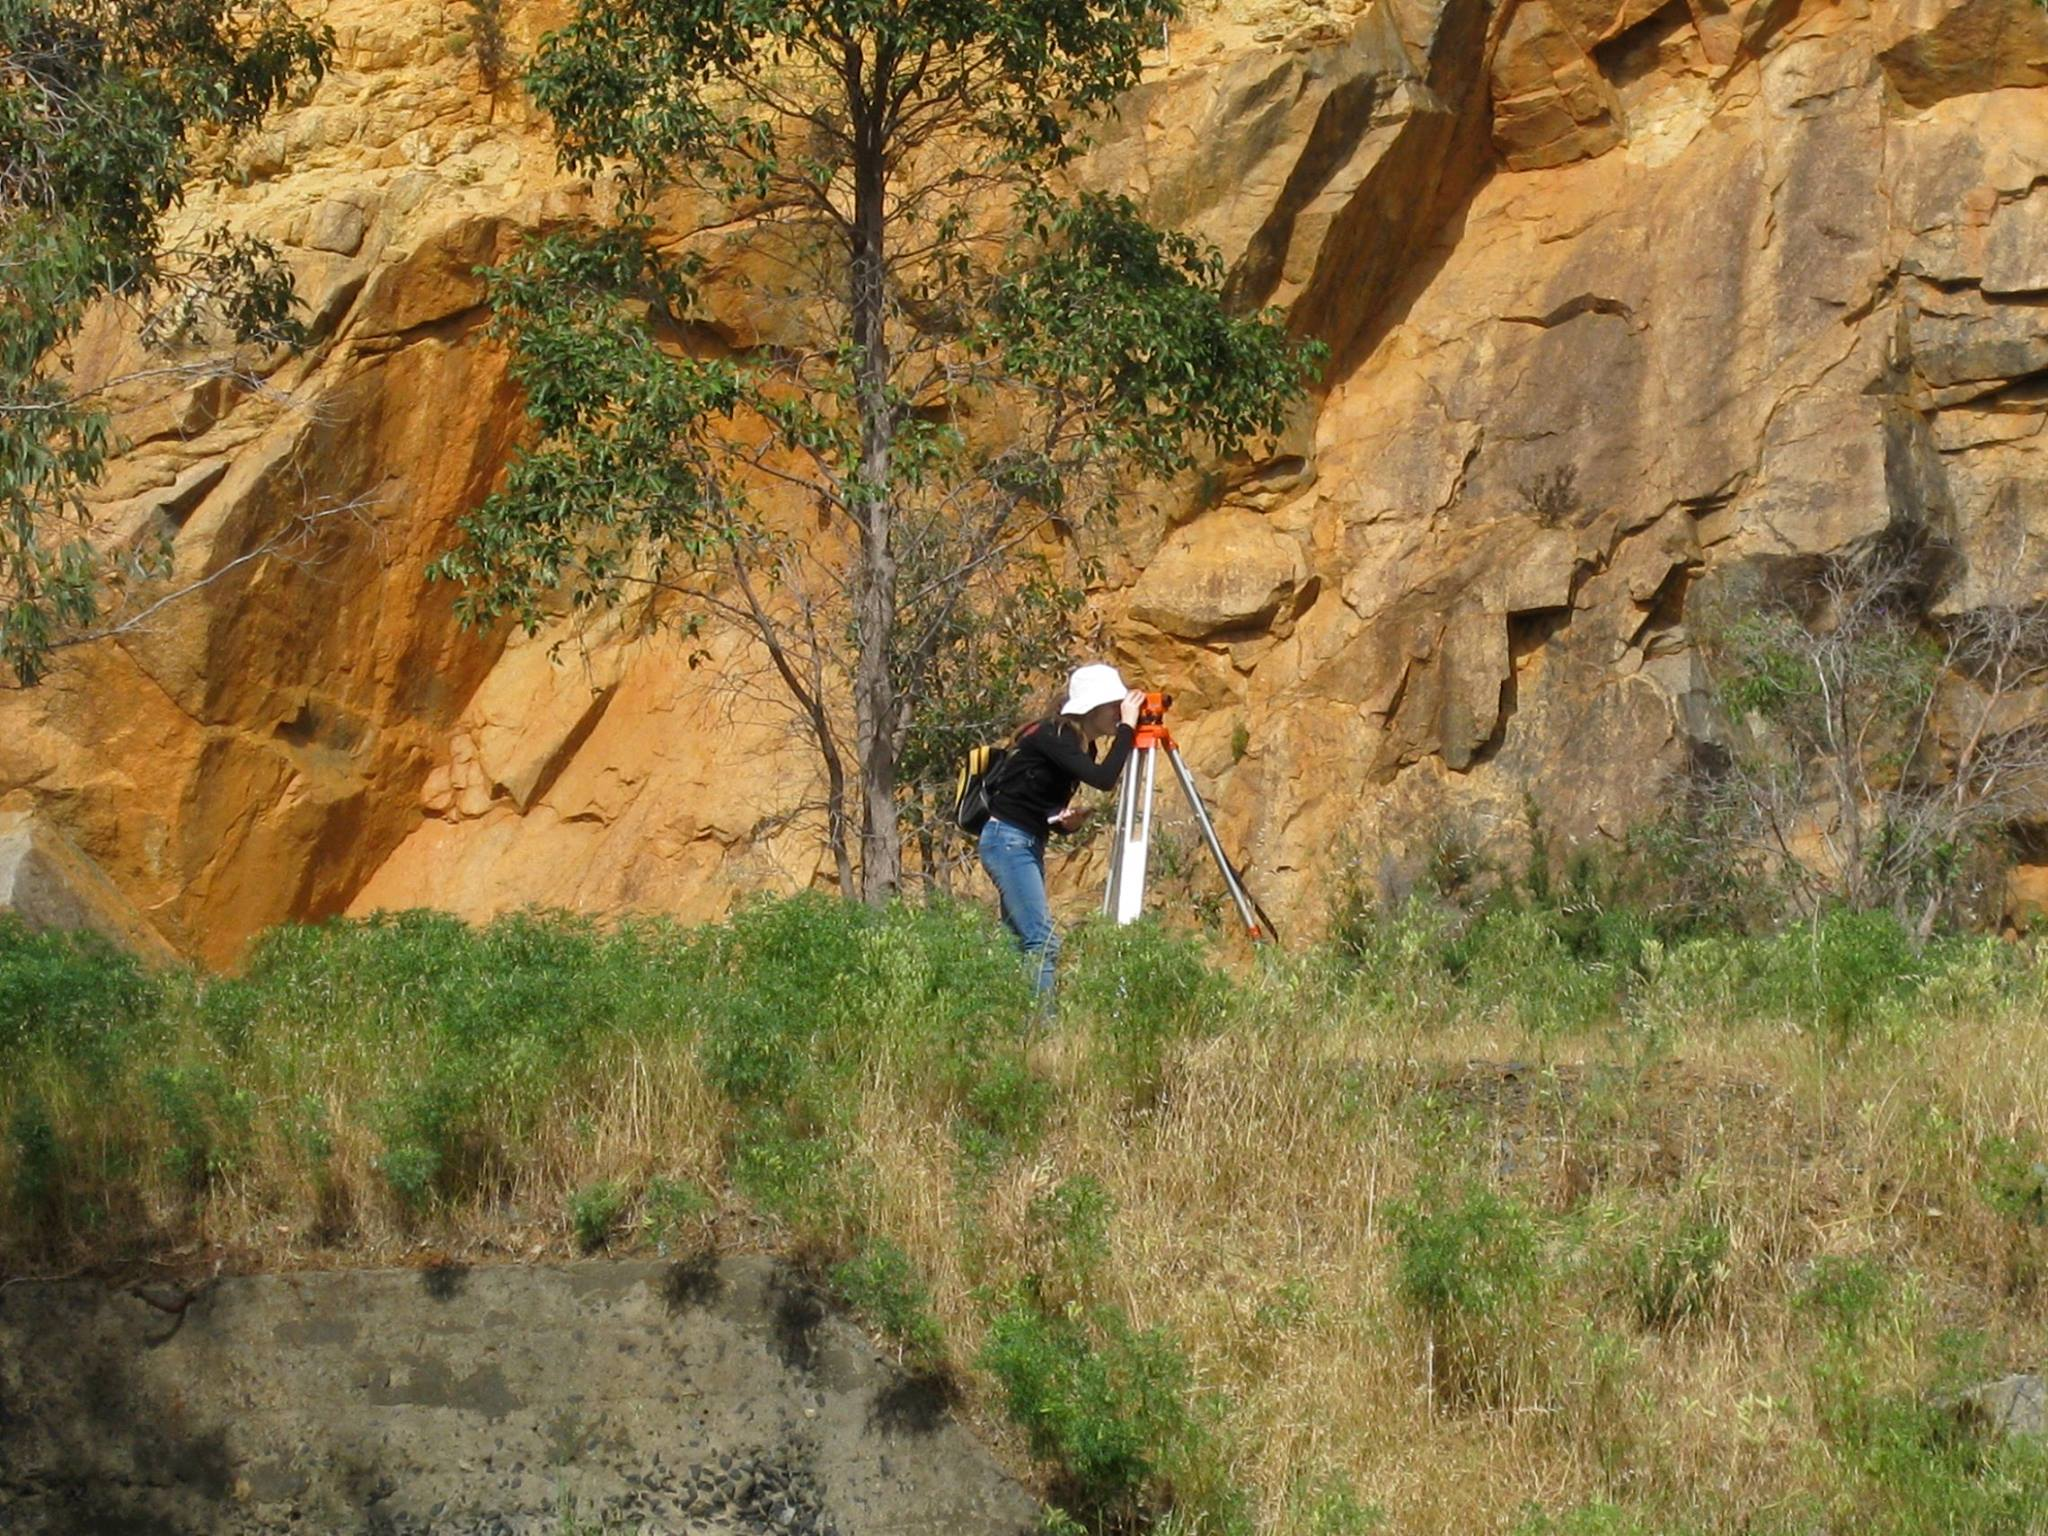
\includegraphics[width=\linewidth]{figures/Fyfe-Figure03}
   		\caption{Revised skills development model.}
   		\centering
   		\label{fig:Fyfe-Figure03}
   	\end{figure}

As planned, a report \parencite{murszewskiwinter2012} was produced by an undergraduate student overseen by a professional archaeologist, 
and a poster \parencite{murszewski2012} was also produced and displayed at the 2012 Australasian Institute for Maritime Archaeology (AIMA)/Australasian Society for Historical Archaeology (ASHA) Conference. 
The model was tested during a further small-scale survey of the Statham’s Quarry site, and used again in the following year in a small historic project for a private landowner, which also resulted in a conference poster \parencite{busher2012}, also for the 2012 AIMA/ASHA Conference.

The model demonstrated that it could provide experiential learning for a large number of students with a wide range of skills in research, fieldwork, analysis and reporting; all of which were applicable to their future employment as well as their current studies. 
With revisions, the model has demonstrated its value. The case studies and subsequent applications show that the model is flexible and responsive to student and community needs. 
Students are able to drive their own involvement in fieldwork, lessening their dependence upon being invited to participate in existing projects. Beyond this, the mentoring relationship between students and professionals allowed students exposure to a wider range of knowledge and experience than might otherwise have been the case.

\section{Discussion}

The need for practical skills in archaeology is essential \parencites{boytner2012}{cobb2012}{colley2012}{mytum2012a}{mytum2012b}{ulm2013} and the model described above is designed to allow students to develop those skills, within a workable, easy to organise, low cost, high participation framework. 
It is driven, not by a university derived curriculum framework, but by students seeking regular participatory access to field experiences. As such, the model may be considered a version of ‘archaeology from below’, a socialist archaeological approach articulated by \textcite{faulkner2000}, in which the participants (the students) are involved in all aspects of the project from design, through to fieldwork and reporting. 
Undergraduate students were, and continue to be, involved at all levels, from identification of the need, development of the project and recruitment of professional archaeologists, to background site research, some supervision and leadership during field days and subsequent report writing.

While overall background development of the projects and mentoring during field days is provided by professional qualified archaeologists, students participate in research design, and in articulating the skills they wish to develop. 
There is variation in the extent of participation by students, with some heavily involved in all aspects, while others limit their involvement to attendance at the field days. 
Typically, those students with an interest in pursuing archaeology as a career are most heavily involved, while those with a more casual interest in the discipline have less investment in the projects. The flexibility of the model allows those varied levels of involvement. The participation of professional archaeologists is similarly variable. 
Qualified archaeologists from a range of backgrounds were approached to provide their time and expertise as volunteers, and people from academia, commercial archaeology, and regulatory bodies, as well as industry and museum departments, volunteered to assist with field days. 
Students were consequently exposed to numerous qualified archaeologists with a range of experience, and this is considered one of the successes of the model. Through this process, the students gained exposure to a range of professional skills and opinions, gaining a wider understanding of approaches to site recording. 
Enterprising students were also able to meet professionals from backgrounds beyond those normally encountered in academia, and to impress potential future employers. 
The success of this exposure to archaeologists from outside academia led ASWA to develop an annual event, dubbed ‘Archy-Con’, inviting archaeologists from a range of backgrounds in Western Australia to meet and share their experiences with students.

The other success of the model is its emphasis on unregistered, often at risk, sites, located on public land. This approach allows the recording of baseline data for sites at risk of immediate destruction. While not considered highly significant, these sites still have the potential to provide useful data to future researchers. 
Significance is a mutable quality \parencites{bowdler1984}{brown2008} and while these sites may not be considered significant now, that may change in future, and this baseline recording provides a heritage service to the Community and the state of Western Australia. 

The insistence that projects be student driven from start to finish, develops an understanding of why archaeology is conducted, as well as how, and emphasises the necessity to practice archaeology within a consistent ethical framework and with a research outcome in mind, rather than simply for the sake of it. 
Fieldwork is configured as the data-gathering phase of a larger archaeological process based on research questions, rather than conducted for its own sake. 

The final phase of the model, post-fieldwork report writing, proved to be one of the less successful aspects. When questioned students suggested they were comfortable conducting background research and fieldwork under supervision, but were much less comfortable writing within the framework of a report. 
This may have been due to unfamiliarity with the format, or the fact that writing their results was more time consuming than other aspects of the project. Regardless, without providing an incentive to do them, reports (or other appropriate outputs) would not have been produced.

From the beginning, the model was developed for best practice in historical archaeology, much of which, in terms of the documentation and recording processes, can be translated to other sub-disciplines within archaeology. 
The general framework of the model of student driven participation in research and fieldwork has been successfully adapted to a number of projects. These include contemporary archaeology projects recording a threatened beach community dating to the 1960's, or recording graffiti in the city of Perth, and a maritime archaeology project recording a shipwreck in shallow water in the Swan River. 
Laboratory projects have also been conducted using this model, with students successfully taking control of, and running, the accessioning and analysis of a number of large artefact assemblages. This has resulted in a range of outputs such as databases, reports, conference posters, submissions to existing heritage registers and artefact catalogues. 
Two papers are also currently in preparation for publication in peer reviewed journals. All of the outputs were produced wholly, or with substantial input, from the student members of ASWA.

One Australian archaeology sub-discipline where the model has not yet been used is Indigenous archaeology. The ethical and regulatory issues associated with working on Indigenous sites in Australia requires a greater level of consultation than those of non-Indigenous sites and these may be better dealt with within the more structured framework of academic and/or consultancy research. 
While the model could be applied to Indigenous sites, a greater degree of planning and consultation, and a multi-year time frame, would be required to meet regulatory requirements and ethical standards.

One difficulty encountered with the model was continuity within ASWA itself. Most students are members for no more than three years and members of the Executive are usually in their positions for only one year, meaning the window for passing on the operation of the model is brief. 
ASWA developed a position within the Executive responsible for liaison with qualified archaeologists in order to continue the organisation of field days; however, the ongoing success of the model has been dependent upon the energy of the office holder. 
Fortunately, longer term postgraduate members of ASWA have allowed a level of knowledge transfer and continuity in the development and application of the model.

\section{Conclusion}

The innovative and structured approach developed by the Archaeological Society of Western Australia and described in this paper, has shown how a flexible approach is essential for a non-academic model, to allow it to be applied to a variety of projects, whilst meeting both the ethical and legal needs consistent with good archaeological practice. 
The model offers real, tangible experiences to students to enhance their skills development and indeed, is driven by the desires and requirements of those students. This project was never intended to replicate or replace highly structured university based practical training; instead, it is designed to allow students to practice skills gained within that structured learning environment. 
The model allows students to initiate and be involved in projects from start to finish, and to tailor their involvement to their level of interest. Despite being tailored to Western Australian conditions, ASWA has developed a model that is flexible and responsive, not restricted by specific legislative requirements. 
It has the potential to be applied wherever there is a strong and motivated student body, professional archaeologists willing to volunteer their time, and sites which are low risk, low significance, accessible, affordable and able to be recorded with minimal impact, and maximum benefit. 

\section{Acknowledgements}

The Discipline of Archaeology at University of Western Australia for the equipment, facilities and laboratory space, and to Jane Balme for feedback on this paper. Thanks to the archaeologists who provided their services as supervisors during field days including Kelly Fleming, State Heritage Office, WA, Alice Beale, WA Museum, Renee Gardiner of Earth Imprints Consulting, Karina Williams of Eureka Archaeological Research and Consulting, Bob Sheppard of Heritage Detection Australia and Stafford Smith. Sarah Knight Regional Program Director ABC Radio for fieldwork and media coverage. Field day volunteers at Canning Mills, and Statham’s Quarry: John Adeney, Samara Allen, Sarah Ames, Natasha Busher, Nina Conway, Lauren Davidson, Matt Dix, Christa Entwhistle, Aaron Floky, Jonathan Gimblett, Alyce Haast, Lisa Hewson, Philipa Hudson, Victoria Kelly, Jess Laurier, Arianne Maggio, Erin Mein, Janet Osborne, Jannie Peircy, Emily Purvis, Malati Redeckis, Rebecca Ryan, Godfrey Rule, Zack Sheppard, Danielle Tassone, Katrina West and Gemma Wilson.

Special thanks to the dedicated and enthusiastic Executive Committees of the Archaeological Society of Western Australia who started this project and have maintained it from 2010 to the present.


\clearpage
\IJSRAclosing
\end{document}
\documentclass{ijsra}

\def\IJSRAidentifier{\currfilebase}
%-------Title | Email | Keywords | Abstract-------------
\def\shorttitle{Late Holocine Rockshelter, Botswana}
\def\maintitle{The Late Holocene Occupation of Mafunyane Shelter, Eastern Botswana}
\def\cmail{tim.forssman@gmail.com}
\def\keywords{Later Stone Age, stone tools, hunter-gatherers, forager-farmer interactions, Greater Mapungubwe Landscape, eastern Botswana}
\def\abstract{Mafunyane \IJSRAsection{Abstract} Shelter is a small rockshelter situated in eastern Botswana along the Limpopo River. The site was occupied from possibly the first centuries \AD until the Leopard’s Kopje period, \AD 1000 to 1300. 
    Excavations revealed an extensive Later Stone Age (LSA) assemblage including stone tools, beads and a diverse faunal record as well as ceramics, a figurine fragment, metal implements, and various metal-working associated finds. Inside the rockshelter is a limited number of rock markings including paintings, cupules and grooves. The site was originally excavated by \textcite{Walker_1994} but until now has not been dated. Here, new findings from a subsequent excavation are presented along with a revised chronological sequence. 
    The occupation of Mafunyane is discussed and the implications relating to the farmer-associated items such as the ceramics and metal assemblage are considered. The results suggest that an expansion of our research approach might reveal aspects of the LSA seldom occurring at large rockshelter sites, such as specific site utilisation patterns, specialist or craft activities, and the variable social responses from forager-farmer interactions.}
%--------Author’s names------------
\def\authorone{Tim Forssman}
%-------Biographical information-------------
\def\bioone{\emph{This paper is the product of DPhil research carried out at the University of Oxford (UK).} \href{https://wits.academia.edu/TimForssman}{Tim Forssman} is a postdoctoral fellow at the University of the Witwatersrand in the Rock Art Research Institute, Johannesburg. His research interests are forager-farmer contact, forager economies and economic contributions, trade dynamics, and rock art. Most recently, Forssmancompleted his doctoral study on forager-farmer relations in eastern Botswana through the University of Oxford.}
%------University/Institution--------------
\def\affilone{Postdoctoral Researcher at the Rock Art Research Institute \\ School of Geography \\ Archaeology and Environmental Studies \\ University of the Witwatersrand (South Africa)}


\begin{filecontents}{\IJSRAidentifier.bib}
@Bachelorthesis{Alexander_1984,
  author = {Alexander, G. J.},
  school = {University of Natal, Pietermaritzburg},
  year   = {1984},
  title  = {A preliminary investigation into the relationships between geology, soils and vegetation in the eastern Tuli Block, Botswana},
  note   = {Unpublished},
}

@Book{Deacon_1984a,
  author    = {Deacon, J.},
  title     = {The Later Stone Age of Southernmost Africa},
  publisher = {British Archaeological Reports},
  location  = {Oxford},
  year      = {1984},
  volume    = {213},
  series    = {BAR International Series},
}

@Inbook{Deacon_1984b,
  author    = {Deacon, J.},
  title     = {Southern African prehistory and paleoenvironment},
  year      = {1984},
  editor    = {Klein, R.},
  publisher = {Balkema},
  chapter   = {Later Stone Age people and their descendants in southern Africa},
  note      = {221-328},
  location  = {Rotterdam},
}

@MastersThesis{Forssman_2010,
  author   = {Forssman, T.},
  title    = {The Later Stone Age occupation and sequence of the Mapungubwe Landscape},
  year     = {2010},
  pubstate = {Unpublished},
  school   = {University of the Witwatersrand, Johannesburg},
}

@Article{Forssman_2013a,
  author  = {Forssman, T.},
  title   = {Missing pieces: the significance of surface scatters on the Mapungubwe Landscape, South Africa},
  volume  = {25},
  pages   = {53-73},
  year    = {2013},
  journal = {Southern African Humanities},
}

@Book{Forssman_2013b,
  author    = {Forssman, T.},
  title     = {Beyond the Dripline: Later Stone Age Changes on the Greater Mapungubwe Landscape},
  publisher = {Lambert Academic Publishing},
  location  = {Saarbrücken},
  year      = {2013},
}


@ARTICLE {Forssman_2013c,
author  = "Forssman, T.",
title   = "A preliminary report on fieldwork in the Northern Tuli Game Reserve, northeastern Botswana",
journal = "South African Archaeological Bulletin",
year    = "2013",
volume  = "68",
pages   = "63-71"
}

@PhdThesis{Forssman_2014a,
  author   = {Forssman, T.},
  title    = {The Spaces between Places: A Landscape Study of Foragers on the Greater Mapungubwe Landscape},
  year     = {2014},
  note     = {Unpublished},
  location = {Oxford},
  school   = {University of Oxford},
}


@ARTICLE {Forssman_2014b,
author  = "Forssman, T.",
title   = "Dzombo Shelter: a contribution to the Later Stone Age sequence of the Greater Mapungubwe Landscape",
journal = "South African Archaeological Bulletin",
year    = "2014",
volume  = "69",
pages   = "182-191"
}


@ARTICLE {Forssman_2015,
author  = "Forssman, T.",
title   = "A macro-fracture investigation of the backed stone tools from Dzombo Shelter, eastern Botswana",
journal = "Journal of Archaeological Science: Reports",
year    = "2015",
volume  = "3",
pages   = "265--274"
}

@Article{Hall_2000,
  author  = {Hall, S. and Smith, B.},
  title   = {Empowering places: rock shelters and ritual control in farmer-forager interactions in the Northern Province},
  volume  = {8},
  pages   = {30--46},
  year    = {2000},
  journal = {South African Archaeological Society Goodwin Series},
}

@Article{Kennett_2002,
  author  = {Kennett, D. and Ingram, B. and Southon, J. and Wise, K.},
  title   = {Differences in 14C age between stratigraphically associated charcoal and marine shell from the archaic period site of Kilometer 4, southern Peru: old wood or old water?},
  volume  = {44},
  pages   = {53-58},
  year    = {2002},
  journal = {Radiocarbon},
}

@Inbook{Kuman_2009,
  author    = {Kuman, K. and Fields, A.},
  title     = {The Cutting Edge: New Approaches to the Archaeology of Human Origins},
  year      = {2009},
  editor    = {Schick and Toth, N.},
  publisher = {Stone Age Institute Press},
  chapter   = {The Oldowan Industry from Sterkfontein Caves, South Africa},
  note      = {159--169},
  location  = {Gosport},
}

@Inbook{Lancaster_2003,
  author    = {Lancaster, S. and Simpson, I. A.},
  title     = {Assessing and modelling faunal turbation},
  year      = {2003},
  volume    = {1111},
  publisher = {British Archaeological Reports},
  pages   = {64--85},
  series    = {BAR International Series},
}


@ARTICLE {Miller_2001,
author  = "Miller, D.",
title   = "Metal assemblages from Greefswald areas K2, Mapungubwe hill and Mapungubwe souther terrace",
journal = "Southern African Archaeological Bulletin",
year    = "2001",
volume  = "56",
pages   = "83--103"
}

@Article{Miller_2002,
  author  = {Miller, D.},
  title   = {Smelter and smith: Iron Age metal fabrication technology in southern Africa},
  volume  = {29},
  pages   = {1083--1131},
  year    = {2002},
  journal = {Journal of Archaeological Science},
}

@ARTICLE {Milleretal_2001,
author  = "Miller, D., Killick, D., van der Merwe, N.",
title   = "Metal working in the Northern Lowveld, South Africa, AD 1000-1890",
journal = "Journal of Field Archaeology",
year    = "2001",
volume  = "28",
pages   = "401--417"
}


@ARTICLE {Orton_2008,
author  = "Orton, J.",
title   = "Later Stone Age ostrich eggshell bead manufacture in the Northern Cape, South Africa",
journal = "Journal of Archaeological Science",
year    = "2008",
volume  = "35",
pages   = "1765--1775"
}

@PhdThesis{Orton_2014,
  author   = {Orton, J.},
  title    = {Late Holocene archaeology in Namaqualand, South Africa: hunter-gatherer and herders in a semi-arid environment},
  year     = {2014},
  note     = {unpublished},
  location = {Oxford},
  school   = {University of Oxford},
}

@Inbook{Reid_1998,
  author    = {Reid, A. and Sadr, K. and Hanson-James, N.},
  title     = {Ditswa mmung: the archaeology of Botswana},
  year      = {1998},
  editor    = {Lane, P. and Reid, A. and Segobye, A.},
  publisher = {Pula Press and the Botswana Society},
  chapter   = {Herding traditions},
  note      = {81--100},
  location  = {Gaborone},
}


@ARTICLE {Schoeman_2006,
author  = "Schoeman, M. H.",
title   = "Imagining rain-places: rain-control and changing ritual landscapes in the Shashe-Limpopo confluence area, South Africa",
journal = "South African Archaeological Bulletin",
year    = "2006",
volume  = "61",
pages   = "152--165"
}

@PhdThesis{vanDoornum_2005,
  author = {{van Doornum}, B.},
  title  = {Changing places, spaces and identity in the Shashe-Limpopo region of Limpopo Province, South Africa},
  year   = {2005},
  note   = {unpublished},
  school = {University of the Witwatersrand, Johanesburg},
}

@Article{vanDoornum_2007,
  author  = {{van Doornum}, B.},
  title   = {Tshisiku Shelter and the Shashe-Limpopo confluence area hunter-gatherer sequence},
  volume  = {19},
  pages   = {17--67},
  year    = {2007},
  journal = {Southern African Humanities},
}

@Article{vanDoornum_2008,
  author  = {{van Doornum}, B.},
  title   = {Sheltered from change: hunter-gatherer occupation of Balerno Main Shelter, Shashe-Limpopo confluence area, South Africa},
  volume  = {20},
  pages   = {249--284},
  year    = {2008},
  journal = {Southern African Humanities},
}

@Article{vanDoornum_2014,
  author  = {{van Doornum}, B.},
  title   = {Balerno Shelter 3: A Later Stone Age site in the Shashe-Limpopo confluence area, South Africa},
  volume  = {29},
  pages   = {129--155},
  year    = {2014},
  journal = {Southern African Humanities},
}


@ARTICLE {Walker_1994,
author  = "Walker, N.",
title   = "The Late Stone Age of Botswana: some recent excavations",
journal = "Botswana Notes and Records",
year    = "1994",
volume  = "26",
pages   = "1--35"
}


@ARTICLE {Wood_2011,
author  = "Wood, M.",
title   = "A glass bead sequence for southern Africa from the 8th to the 16th century AD",
journal = "Journal of African Archaeology",
year    = "2011",
volume  = "9",
pages   = "67--84"
}
\end{filecontents}

%--------------------------------------------------------------
\begin{document}
\IJSRAopening

%\section{Introduction}
\lettrine{T}{he} Later Stone Age (LSA) sequence of the Greater Mapungubwe Landscape, which includes parts of eastern Botswana, northern South Africa and south-western Zimbabwe (\cref{fig:Forssman-Figure01}), has been at the centre of a number of studies \parencites[e.g.][]{Hall_2000,vanDoornum_2005,vanDoornum_2007,vanDoornum_2008,vanDoornum_2014,Forssman_2010,Forssman_2013a,Forssman_2013b,Forssman_2013c,Forssman_2014a,Forssman_2014b}. 
Most have been restricted to large rockshelter sites in South Africa, and from this work a fairly comprehensive occupation sequence has been established. In an attempt to expand upon this, the author conducted research in eastern Botswana where a series of sites including open-air camps, small or discrete rockshelters and homesteads containing LSA stone artefacts were excavated. The aim of this study was to develop a regional understanding of the local LSA sequence and perform trans-national research, crossing modern boundaries that may not have been present in the past but which potentially confine our work today \parencites[for details see][]{Forssman_2014a}{Forssman_2014b}{Forssman_2013c}{Forssman_2015}. One of the excavated sites, Mafunyane Shelter, is a small rockshelter originally excavated by \textcite{Walker_1994} as Tuli Lodge. 
In new excavations at the site an archaeological assemblage was uncovered that offered an additional perspective on landscape patterns, forager-farmer interactions and metal-working. Presented here are these results.
	
\begin{figure}
		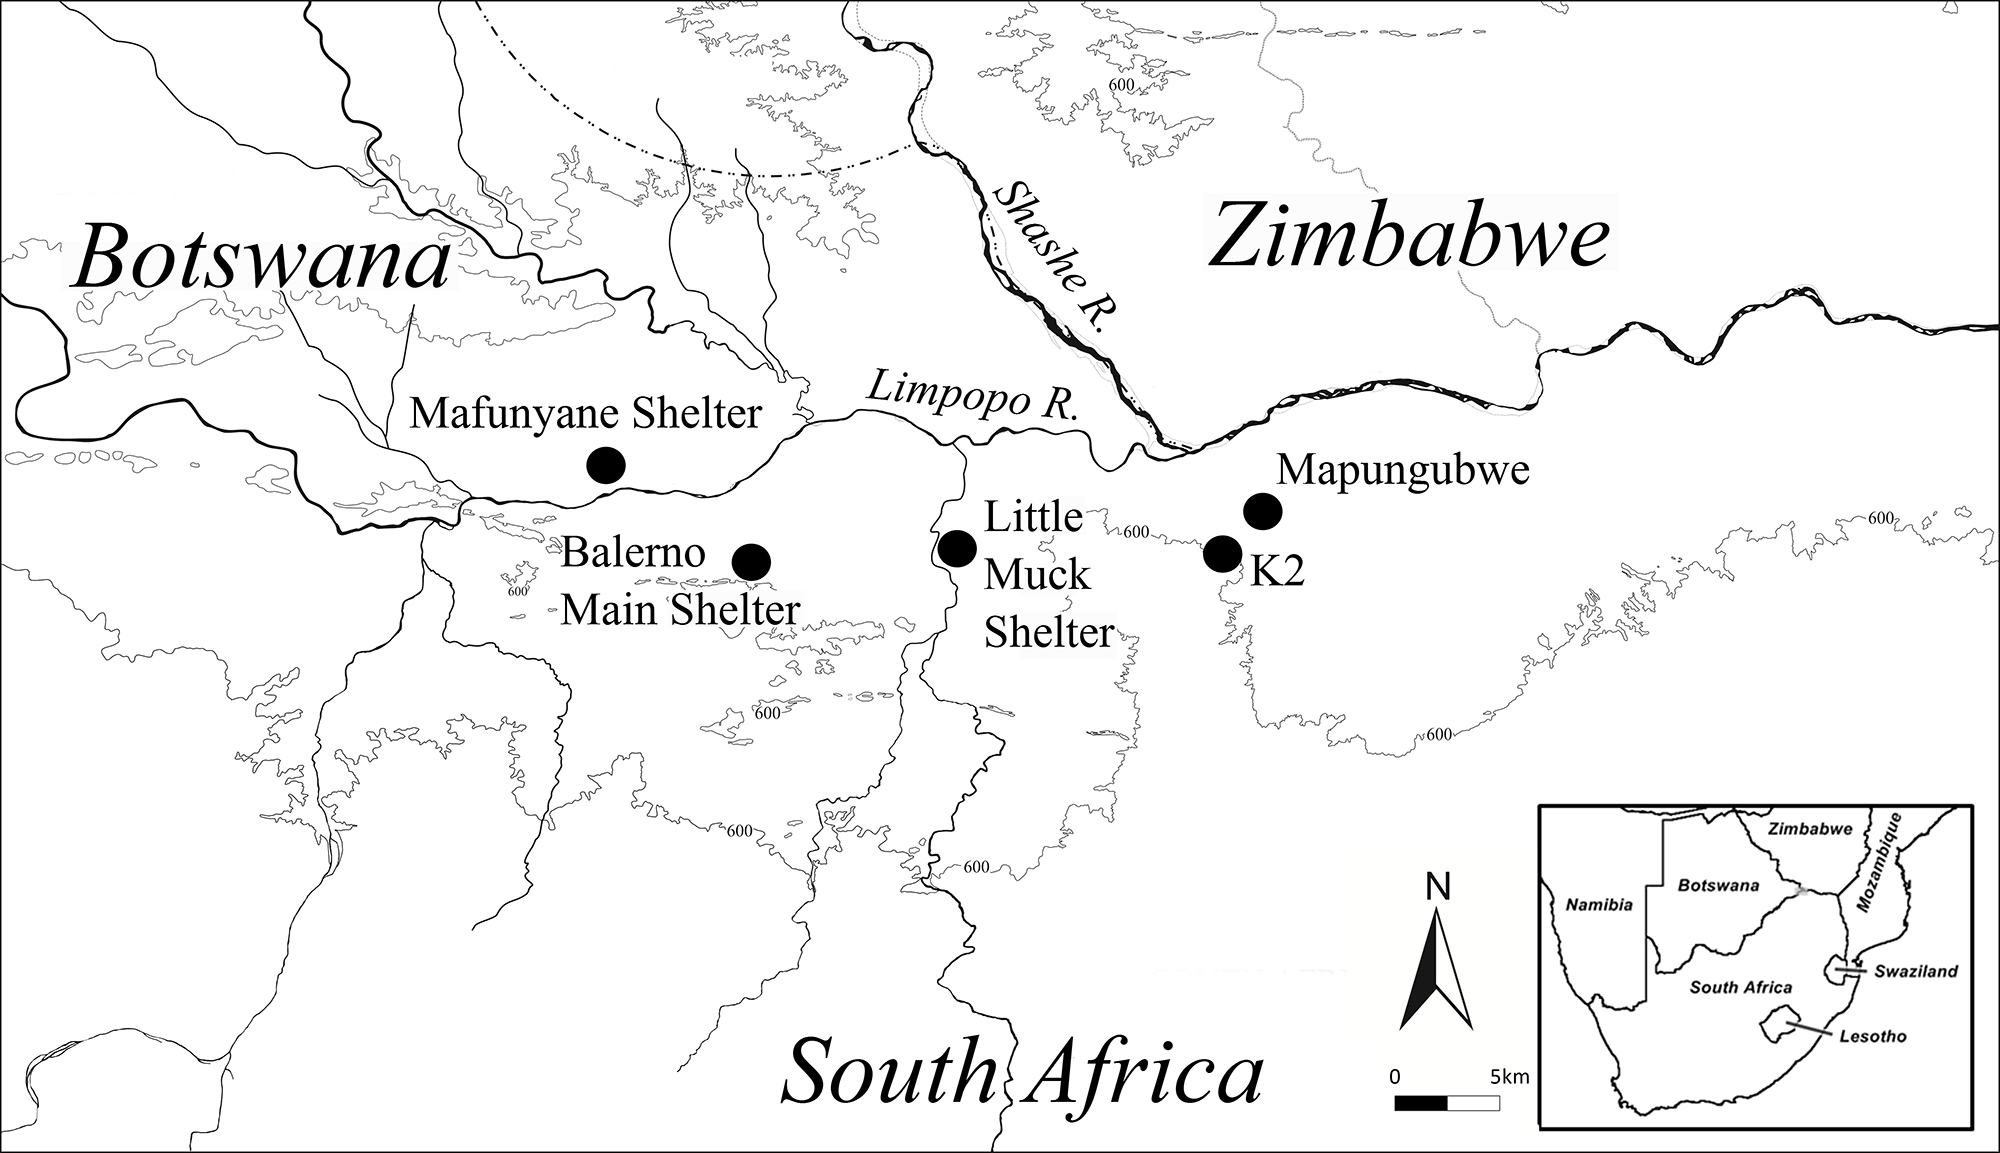
\includegraphics[width=\linewidth]{Forssman-Figure01}
 \caption{The Greater Mapungubwe Landscape with sites mentioned in the text and other prominent sites.
     {\normalfont \\ \copyright\ by NAME OF COPYRIGHT HOLDER}}
		\label{fig:Forssman-Figure01}
\end{figure}

Mafunyane \IJSRAsection{Mafunyane Shelter} is situated in a sandstone belt that stretches along the Motloutse, Limpopo, and Shashe Rivers. Within this area are low-lying koppies (sandstone inselbergs) and ridges interspersed with water networks and small floodplains. The area immediately surrounding the site is characterised by a fine loam to clay soil horizon, created by depositional processes from flooding by the Limpopo River, \SI{460}{\meter} away, and a nearby seasonal stream. 
	The vegetation around the site is characterised by dense pockets of mopane veld (\emph{Colophospermum mopane}) and more widespread vachellia and acacia open shrubland. The site’s near proximity to the Limpopo River suggests that in the past the immediate area may have been a riverine woodland, which today is restricted to the banks of major rivers due to the receding water table \parencite{Alexander_1984}. 
	
	\textcite{Walker_1994} previously excavated the site under the name Tuli Lodge. It was not known at first whether Mafunyane was the \textcite{Walker_1994} site because no GPS co-ordinates were published and at the time of this study the reserve management had not been informed of his research on the farm. Once it was established that the sites were the same it was decided to re-excavate the rockshelter in order to increase the site’s sample size, obtain charcoal samples for radiocarbon dating and relate the findings made here to the broader regional sequence. \textcite{Walker_1994} recovered an extensive LSA assemblage including \num{14379} stone tools along with 21 pieces of worked bone, fragments from tortoise and ostrich eggshell bowls and containers, 67 ostrich eggshell beads, 64 potsherds, a pipe and crucible, six glass trade beads and 16 metal implements as well as large amounts of metal prills. 
	He concluded that based on the prevalence of scrapers in the assemblage, the site was occupied from probably the first few centuries \AD, and that the foragers using the site were in contact with farmers. 
In addition, he states that the rockshelter was \enquote{clearly a major living site} that 
	\enquote{was probably seasonally occupied, but it was later used by metalworking people to smelt copper} \parencite[10]{Walker_1994}. 
	
%\section*{Excavation, Stratigraphy, and Chronology}
The site’s floor was \IJSRAsection{Excavation, Stratigraphy, and Chronology} divided into a grid of \SIrange{1}{1}{\meter} squares with alphabetical designations running east to west and numeric designations running south to north. 
Square 3C was selected for excavations primarily because it was located in an area most likely to contain a deep and intact deposit (\cref{fig:Forssman-Figure02}). 
On excavating the square it was found that a portion of it, the southwestern quadrant, protruded into what appeared to be the \textcite{Walker_1994} excavation and so this quadrant was excluded; 
thus only three quadrants were excavated to bedrock. Initially excavations were also to be conducted in the large open-air living area north of the site, but this area was found to contain little deposit and appeared highly disturbed. 
Excavations therefore only proceeded inside the rockshelter and were conducted in spits of \SI{30}{\milli\meter} following natural stratigraphic units.

	\begin{figure}
		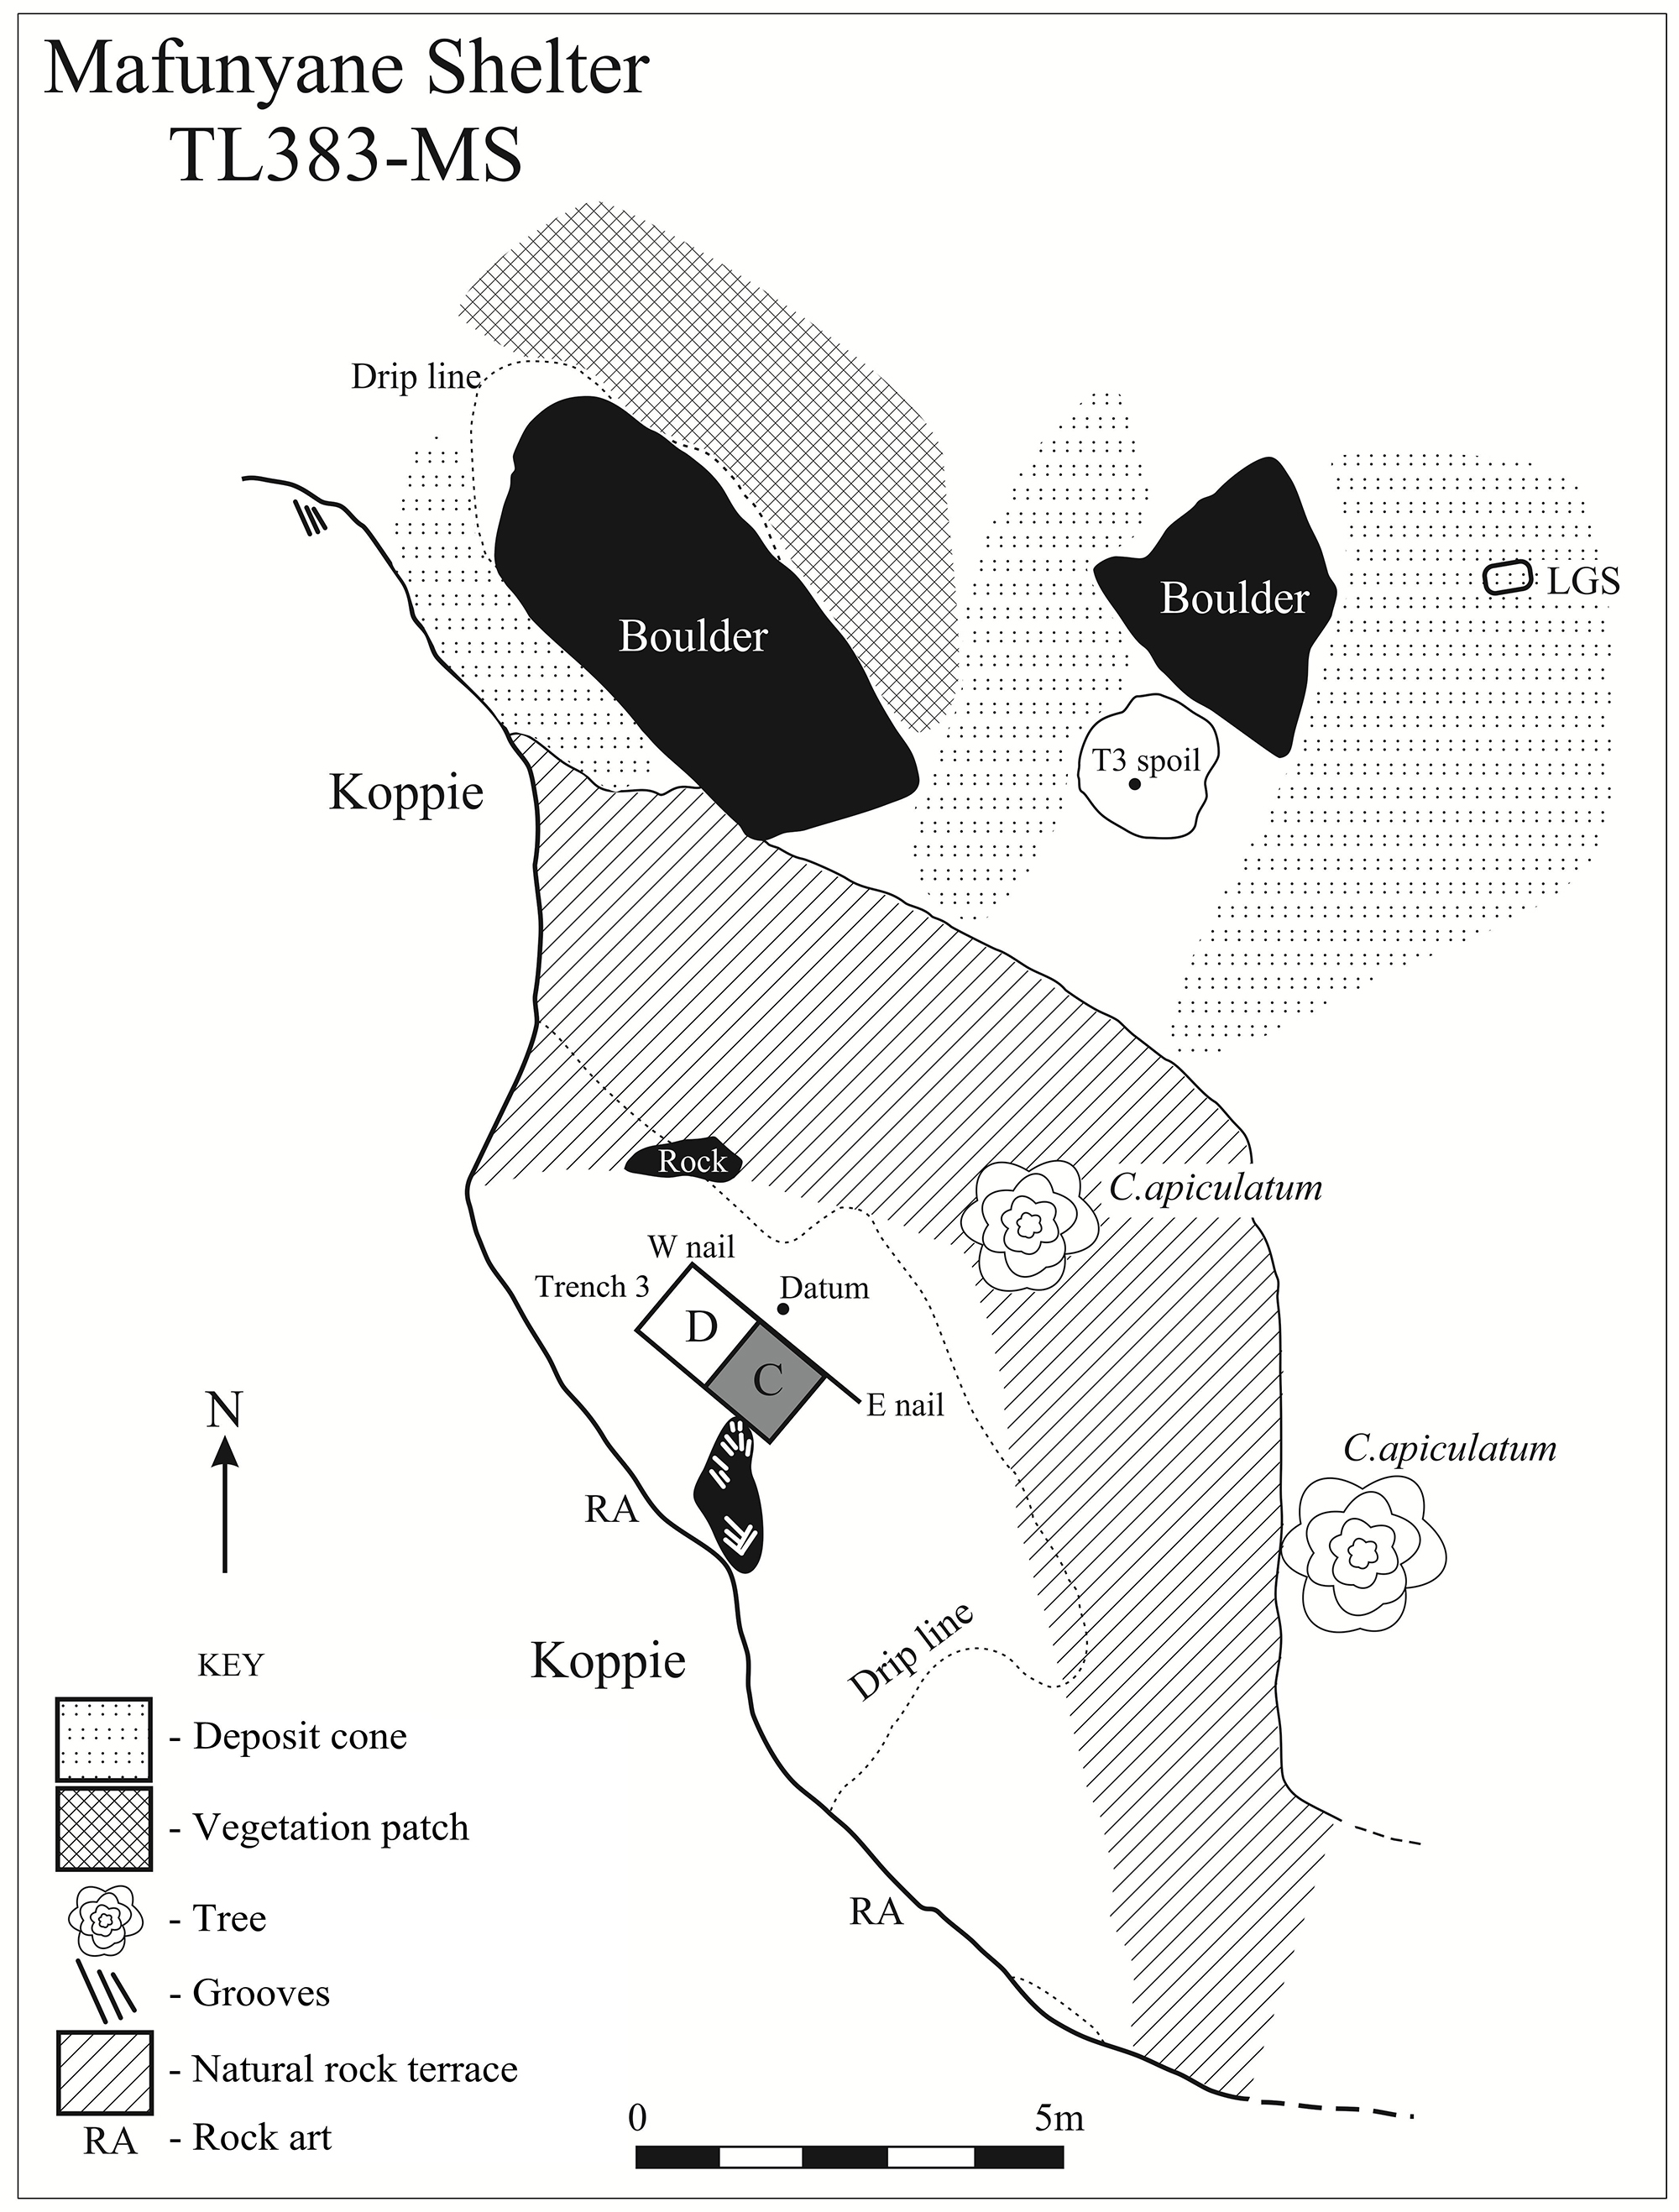
\includegraphics[width=\linewidth]{figures/Forssman-Figure02}
		\caption{Only Square C was excavated at Mafunyane since Square D protruded into the \textcite{Walker_1994} excavation, not visible on the surface but recorded once the surface layer was removed \parencite[from][96]{Forssman_2014a}.}
		\label{fig:Forssman-Figure02}
	\end{figure}

In total seven spits between the surface and bedrock were excavated, revealing three stratigraphic layers, each distinct from the other and similar to \textcite{Walker_1994}. 
The upper most layer, Pale brown sand (PBS), contains small (<\SI{25}{\milli\meter}) sandstone pebbles in an unconsolidated deposit,
 less than \SI{6}{\centi\meter} thick filling \num{2,3} buckets (\SI{13}{\liter} each). 
PBS occurred in Spit I-III but from Spit II, Ashy sand (AS) appears and may be a hearth layer. 
This layer is ash grey, loosely consolidated, with few to no pebbles and is also about \SI{6}{\centi\meter} in thickness (\num{3.4} buckets). 
The lowermost layer, Stony-ashy sand (SAS), is the most substantial (± \SI{12}{\centi\meter} in thickness; \num{4.5} buckets) and also appears to be a hearth with a similar colour to AS but with considerably more pebbles and stones included in the deposit (\cref{fig:Forssman-Figure03}). The depth of bedrock was on average \SI{20}{\centi\meter} below the surface and a total of \num{10.3} buckets was removed from the site \parencite[for more details see][95]{Forssman_2014a}. 

	\begin{figure}
		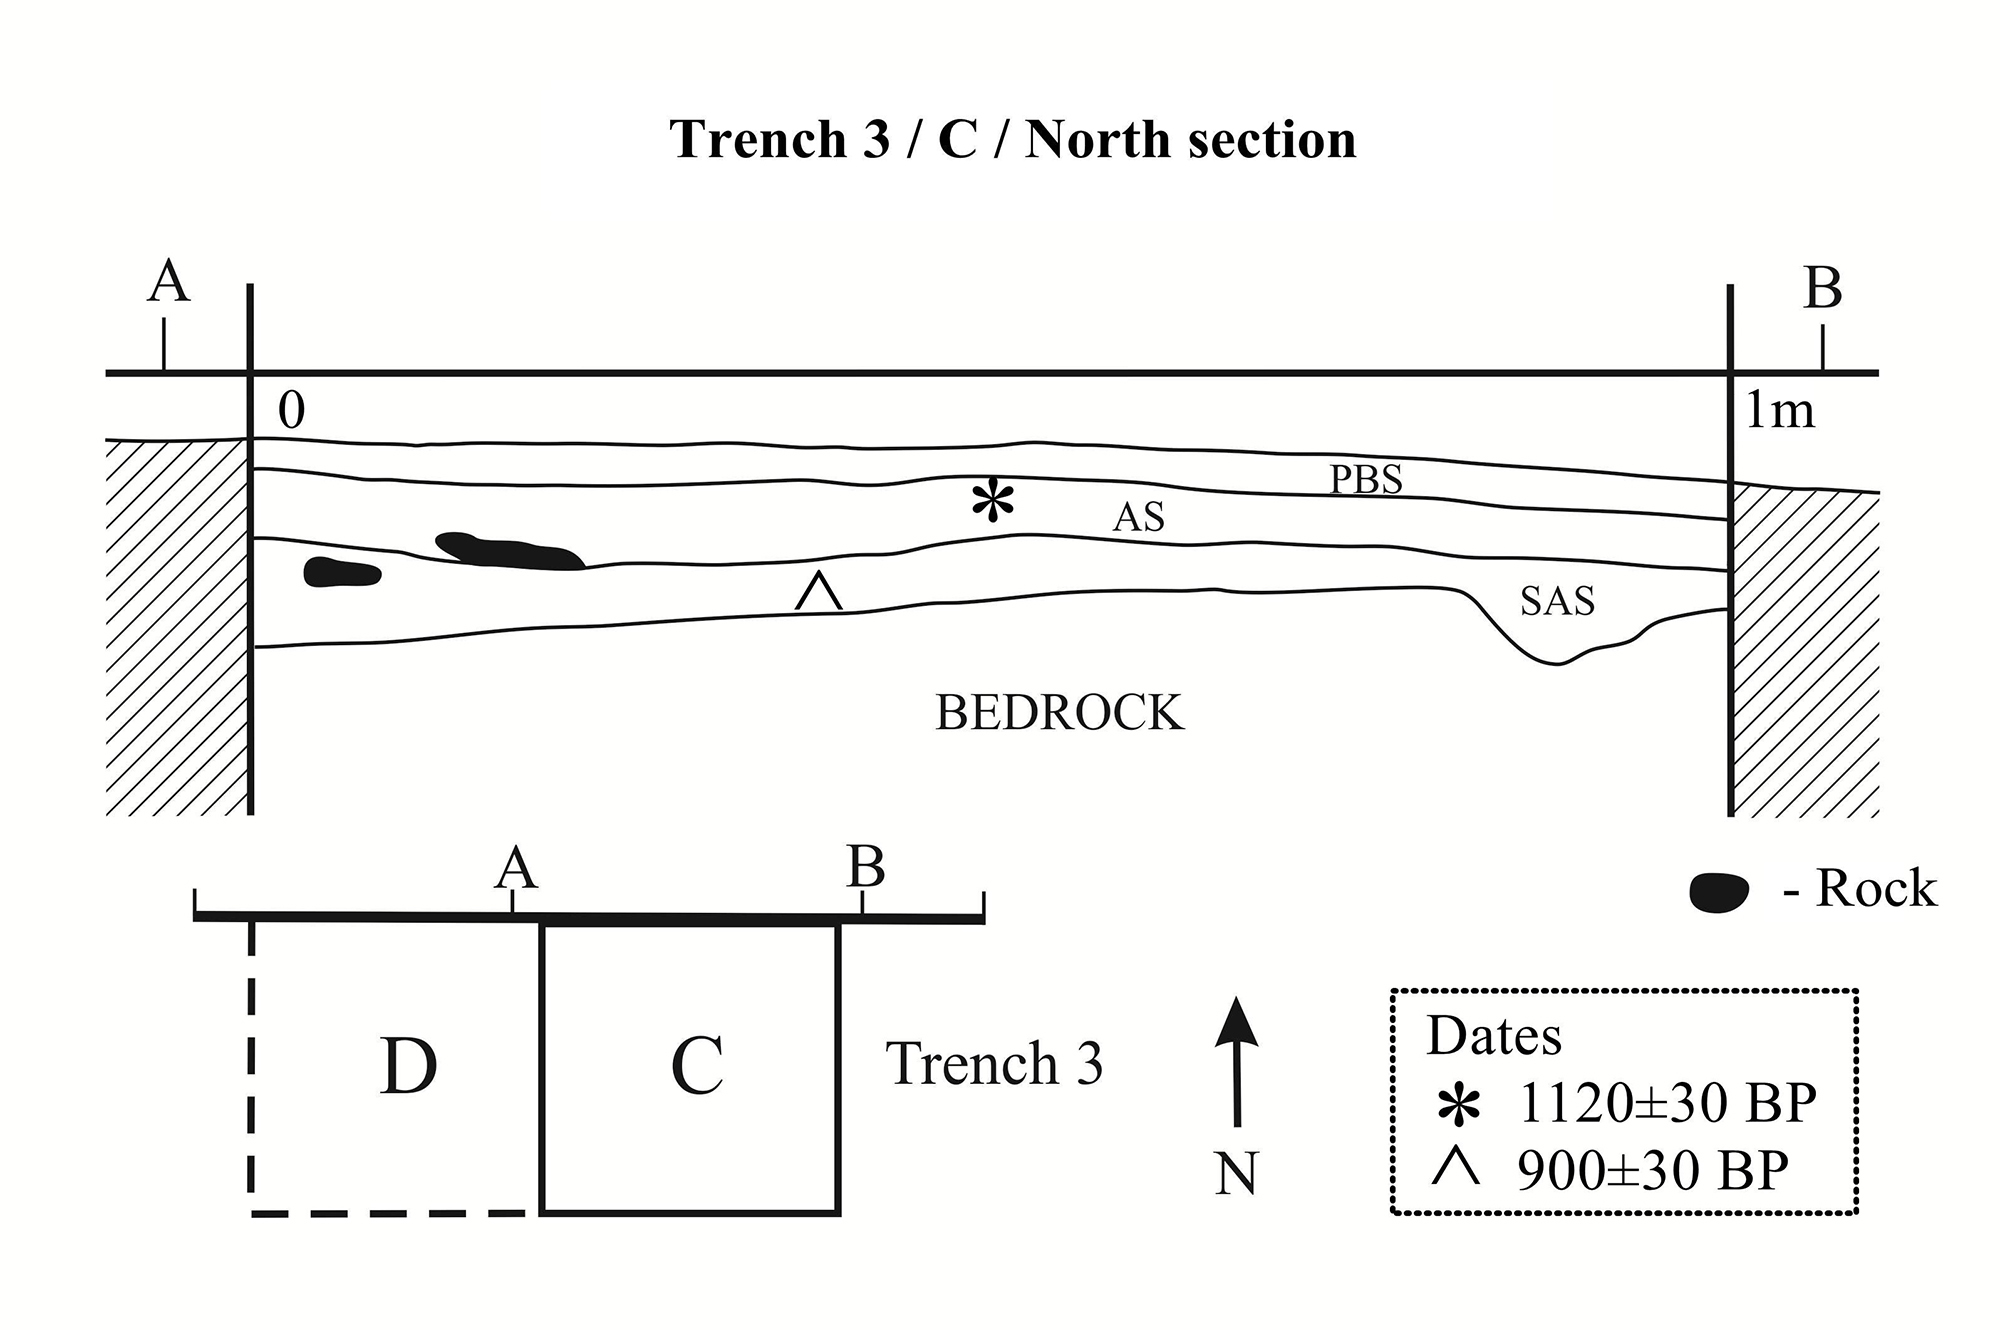
\includegraphics[width=\linewidth]{figures/Forssman-Figure03}
		\caption{Section drawing of the north wall in Square C at Mafunyane indicating the approximate location of the radiocarbon dates.}
		\centering
		\label{fig:Forssman-Figure03}
	\end{figure}

Two charcoal samples were submitted for radiocarbon dating to Beta Analytic and the results are presented in \cref{fig:Forssman-Table01}. 
The samples indicate that the site was occupied between \AD 941 and 1265. 
However, the more recent date is from Spit VII and the older from Spit II. 
The laboratory did not find any evidence indicating that the samples were possibly contaminated and so this does not seem to have caused the inverted dates. 
It is possible that the sample from Spit VII is ‘old wood’, which introduces an unresolvable variable into the calibration process \parencite{Kennett_2002}, but could equally have moved after deposition, possibly due to bioturbation \parencite[see][]{Lancaster_2003} or root action in the deposit (roots were recorded above bedrock). 
Ceramics do little to assist, although they appear to be contemporaneous (discussed below), and no other chronological markers were identified in the relevant spits. Therefore, the integrity of the deposit is uncertain (but see discussion below).

	\begin{figure} %TABLE 1
		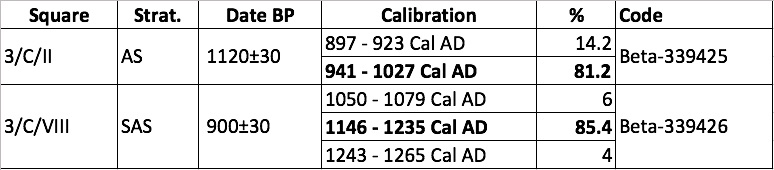
\includegraphics[width=\linewidth]{figures/Forssman-Table01}
		\captionof{table}{Calibrated radiocarbon dates on charcoal samples from Mafunyane.}
		\label{fig:Forssman-Table01}
	\end{figure}

%\section*{The Stone Tool Assemblage}

Square C \IJSRAsection{The Stone Tool Assemblage} produced a total of \num{6349} stone tools within \num{10.3} buckets (\SI{0.1}{\meter\cubed}). 
As with other rockshelter excavations in the area, the assemblage is dominated by crypto-crystalline silicates (CCS), 
after which quartz follows and then consistently low frequencies of quartzite, agate and dolerite (\cref{fig:Forssman-Table02}). 
The greatest number of stone artefacts is found between Spits II and V, 
followed by a decrease until bedrock is reached in Spit VII (\cref{fig:Forssman-Figure04}).
A similar pattern was noted with regard to the stone tool density (artefacts/\SI{13}{\liter} bucket) with the exception of the high density on the surface and in Spit I. 
If the high density of stone tools on the surface represents a forager use of the rockshelter, it may be after \AD 1200 based on the radiocarbon dates and the Leopard’s Kopje ceramics found by \textcite{Walker_1994} in the upper levels of his excavation. 


	\begin{figure} %Figure 4
		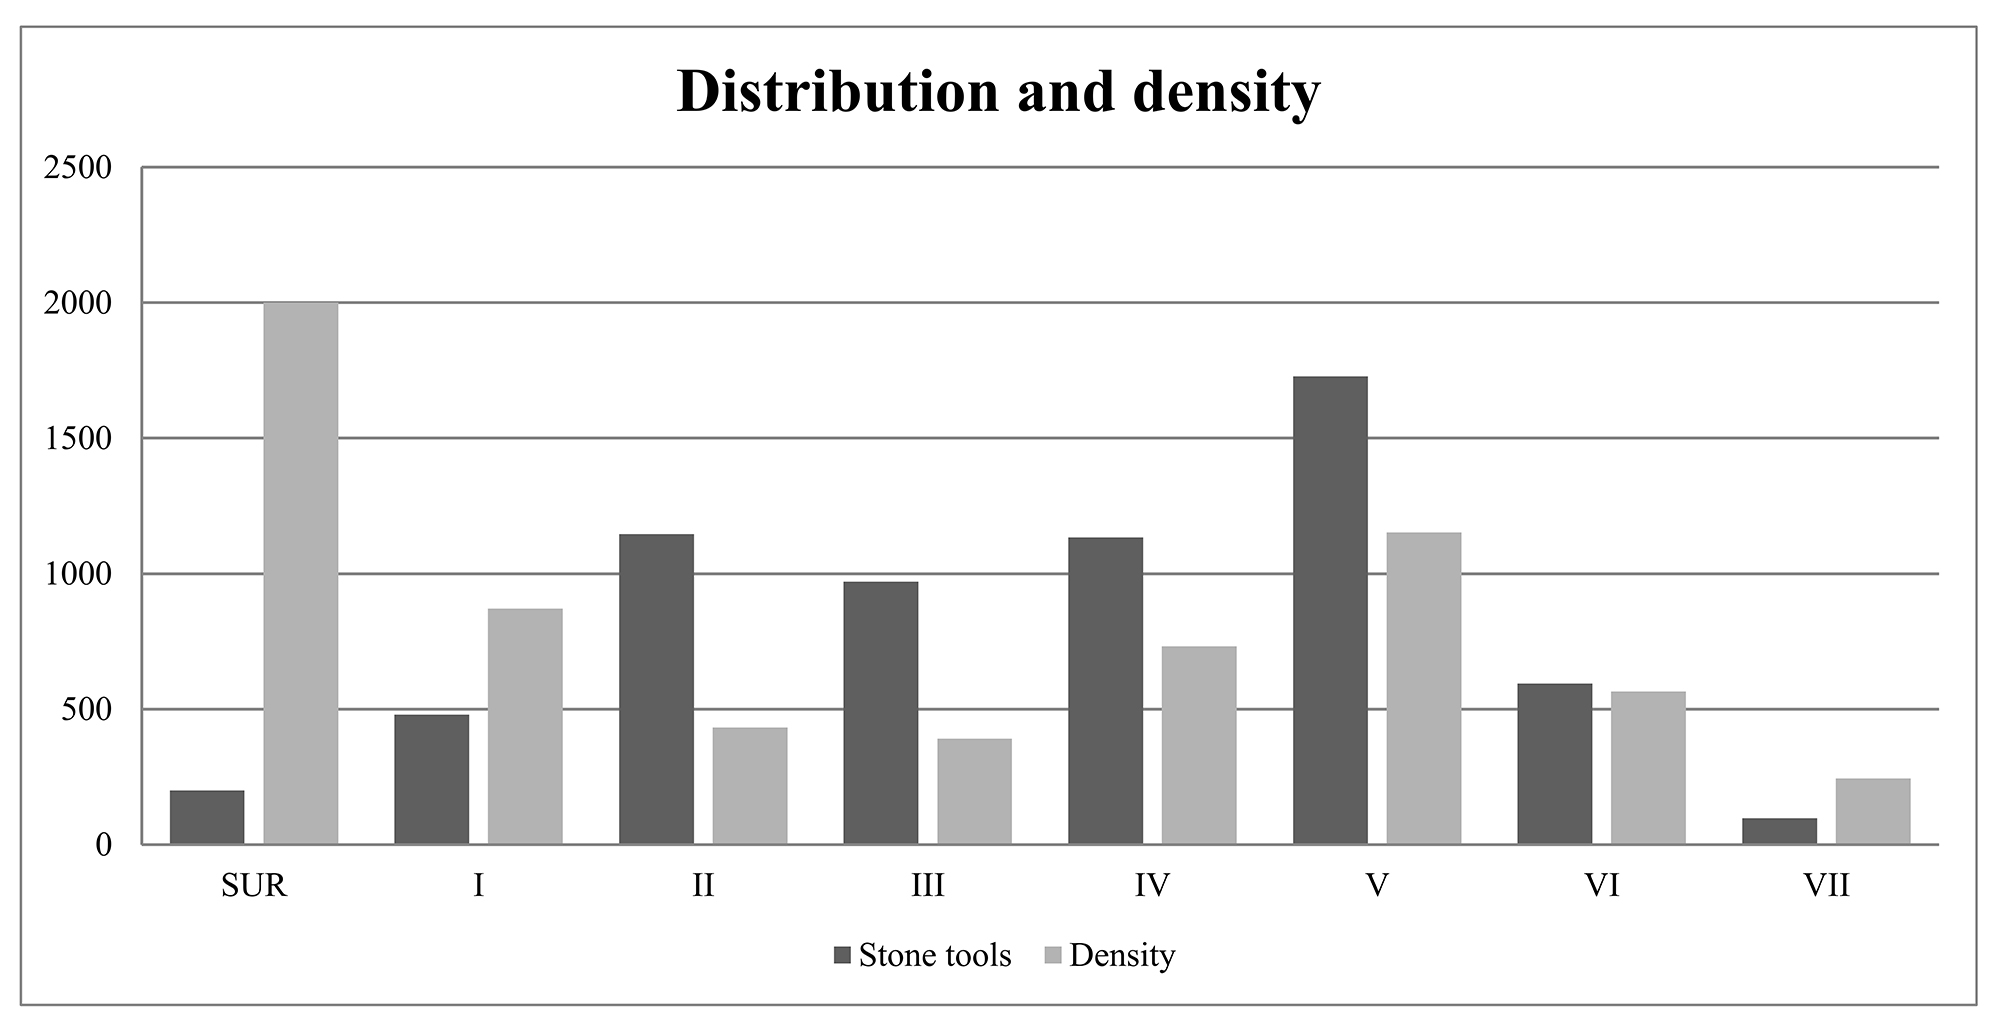
\includegraphics[width=\linewidth]{figures/Forssman-Figure04}
		\caption{The distribution and density (artefacts/\SI{13}{\liter} bucket) of stone tools at Mafunyane.}
		\label{fig:Forssman-Figure04}
	\end{figure}

	\begin{figure} %TABLE 2
		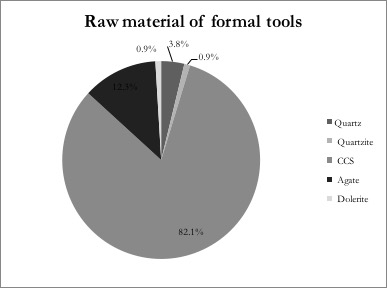
\includegraphics[width=\linewidth]{figures/Forssman-Table02}
		\captionof{table}{Raw material use through the spits and total stone tool distribution.}
		\label{fig:Forssman-Table02}
	\end{figure}

Below the stone tool assemblage has been separated into two categories based on the typological breakdown from \textcite{Walker_1994}: 1) debitage and utilised pieces and 2) formal tools.

%\subsection*{Debitage and utilised pieces}
Debitage are \IJSRAsection{Debitage and utilised pieces} pieces that might have been used but do not contain secondary working. 
At Mafunyane, this amounts to \SI{98.3}{\percent} of the rockshelter’s total stone tool assemblage (n=\num{6242}). 
The majority of these are chips, comprising of \num{3391} artefacts and \SI{53.4}{\percent} of the total assemblage. 
Chips measure less than \SI{10}{\milli\meter}
  in length and do not contain secondary working or high utilisation damage \parencite[see][]{Deacon_1984a}. 
 The presence of chips indicates that a) the deposit has not been exposed to high levels of colluvial action \parencite{Kuman_2009} and b) primary stone tool knapping occurred at the site.

There are 82 cores (\SI{1.3}{\percent}) and most were found in Spits IV and V, part of SAS, totalling 52 artefacts and \SI{63.4}{\percent} of the core category. 
Irregular cores are the most frequent core type (n=37). 
This is followed by single platform and rice seed (n=10 each), casual (n=9), preliminary flaked (n=8), bipolar bladelet (n=3), radial (n=2) and bipolar, bipolar radial and opposed platform cores (n=1 each). 
The bipolar, radial and rice seed cores indicate that a bipolar flaking technique was used \parencite[see][]{vanDoornum_2005}
 and total 15 artefacts. 
 \textcite[259]{vanDoornum_2008} found that at Balerno Main Shelter bipolar flaking increased from the beginning of contact with farming (agropastoralist) communities in the first centuries\AD. 
 It is not possible to draw the same conclusion at Mafunyane since the site appears to have been occupied for only a short phase within this period.
 
 %/subsection*{Formal Tools}
 The formal tool assemblage, which totals 107 \IJSRAsection{Formal Tools} artefacts (\SI{1.7}{\percent}), 
is not unlike other LSA assemblages in the area \parencite{vanDoornum_2005}(\cref{fig:Forssman-Figure05}). 
Most of the formal tools were produced using CCS materials (\cref{fig:Forssman-Figure06})
  and were found in Spits IV and V, after which they decrease until bedrock is reached in Spit VII. Stratigraphically it is the lowermost unit, SAS, that contains the majority of the formal tools (n=79; \SI{73.8}{\percent}). 
  Scraping tools (\SI{57}{\percent}), of which there are 11 different forms,
   dominate the formal tool assemblage and fall into three size classes: 
   small (<\SI{20}{\milli\meter}; n=51; \SI{83.6}{\percent}), 
   medium (\SIrange{20}{30}{\milli\meter}; n=6; \SI{9.8}{\percent}) and large (>\SI{30}{\milli\meter}; n=4; \SI{6.6}{\percent}; 
   \cref{fig:Forssman-Table03}). 
 Also frequent are backed stone tools (\SI{25.2}{\percent}), a category which includes segments in various stages of completion (n=12), 
whole (n=10) and broken (n=1) segmented backed bladelets and two broken and one complete backed bladelet. 
The only other tools found at Mafunyane were adzes (n=5) possibly used for woodworking \parencite{Walker_1994}, awls (n=2) associated with boring activities \parencite{Deacon_1984a}, and miscellaneous backed pieces (MBP; n=11). 
   
	\begin{figure} %Figure 5
		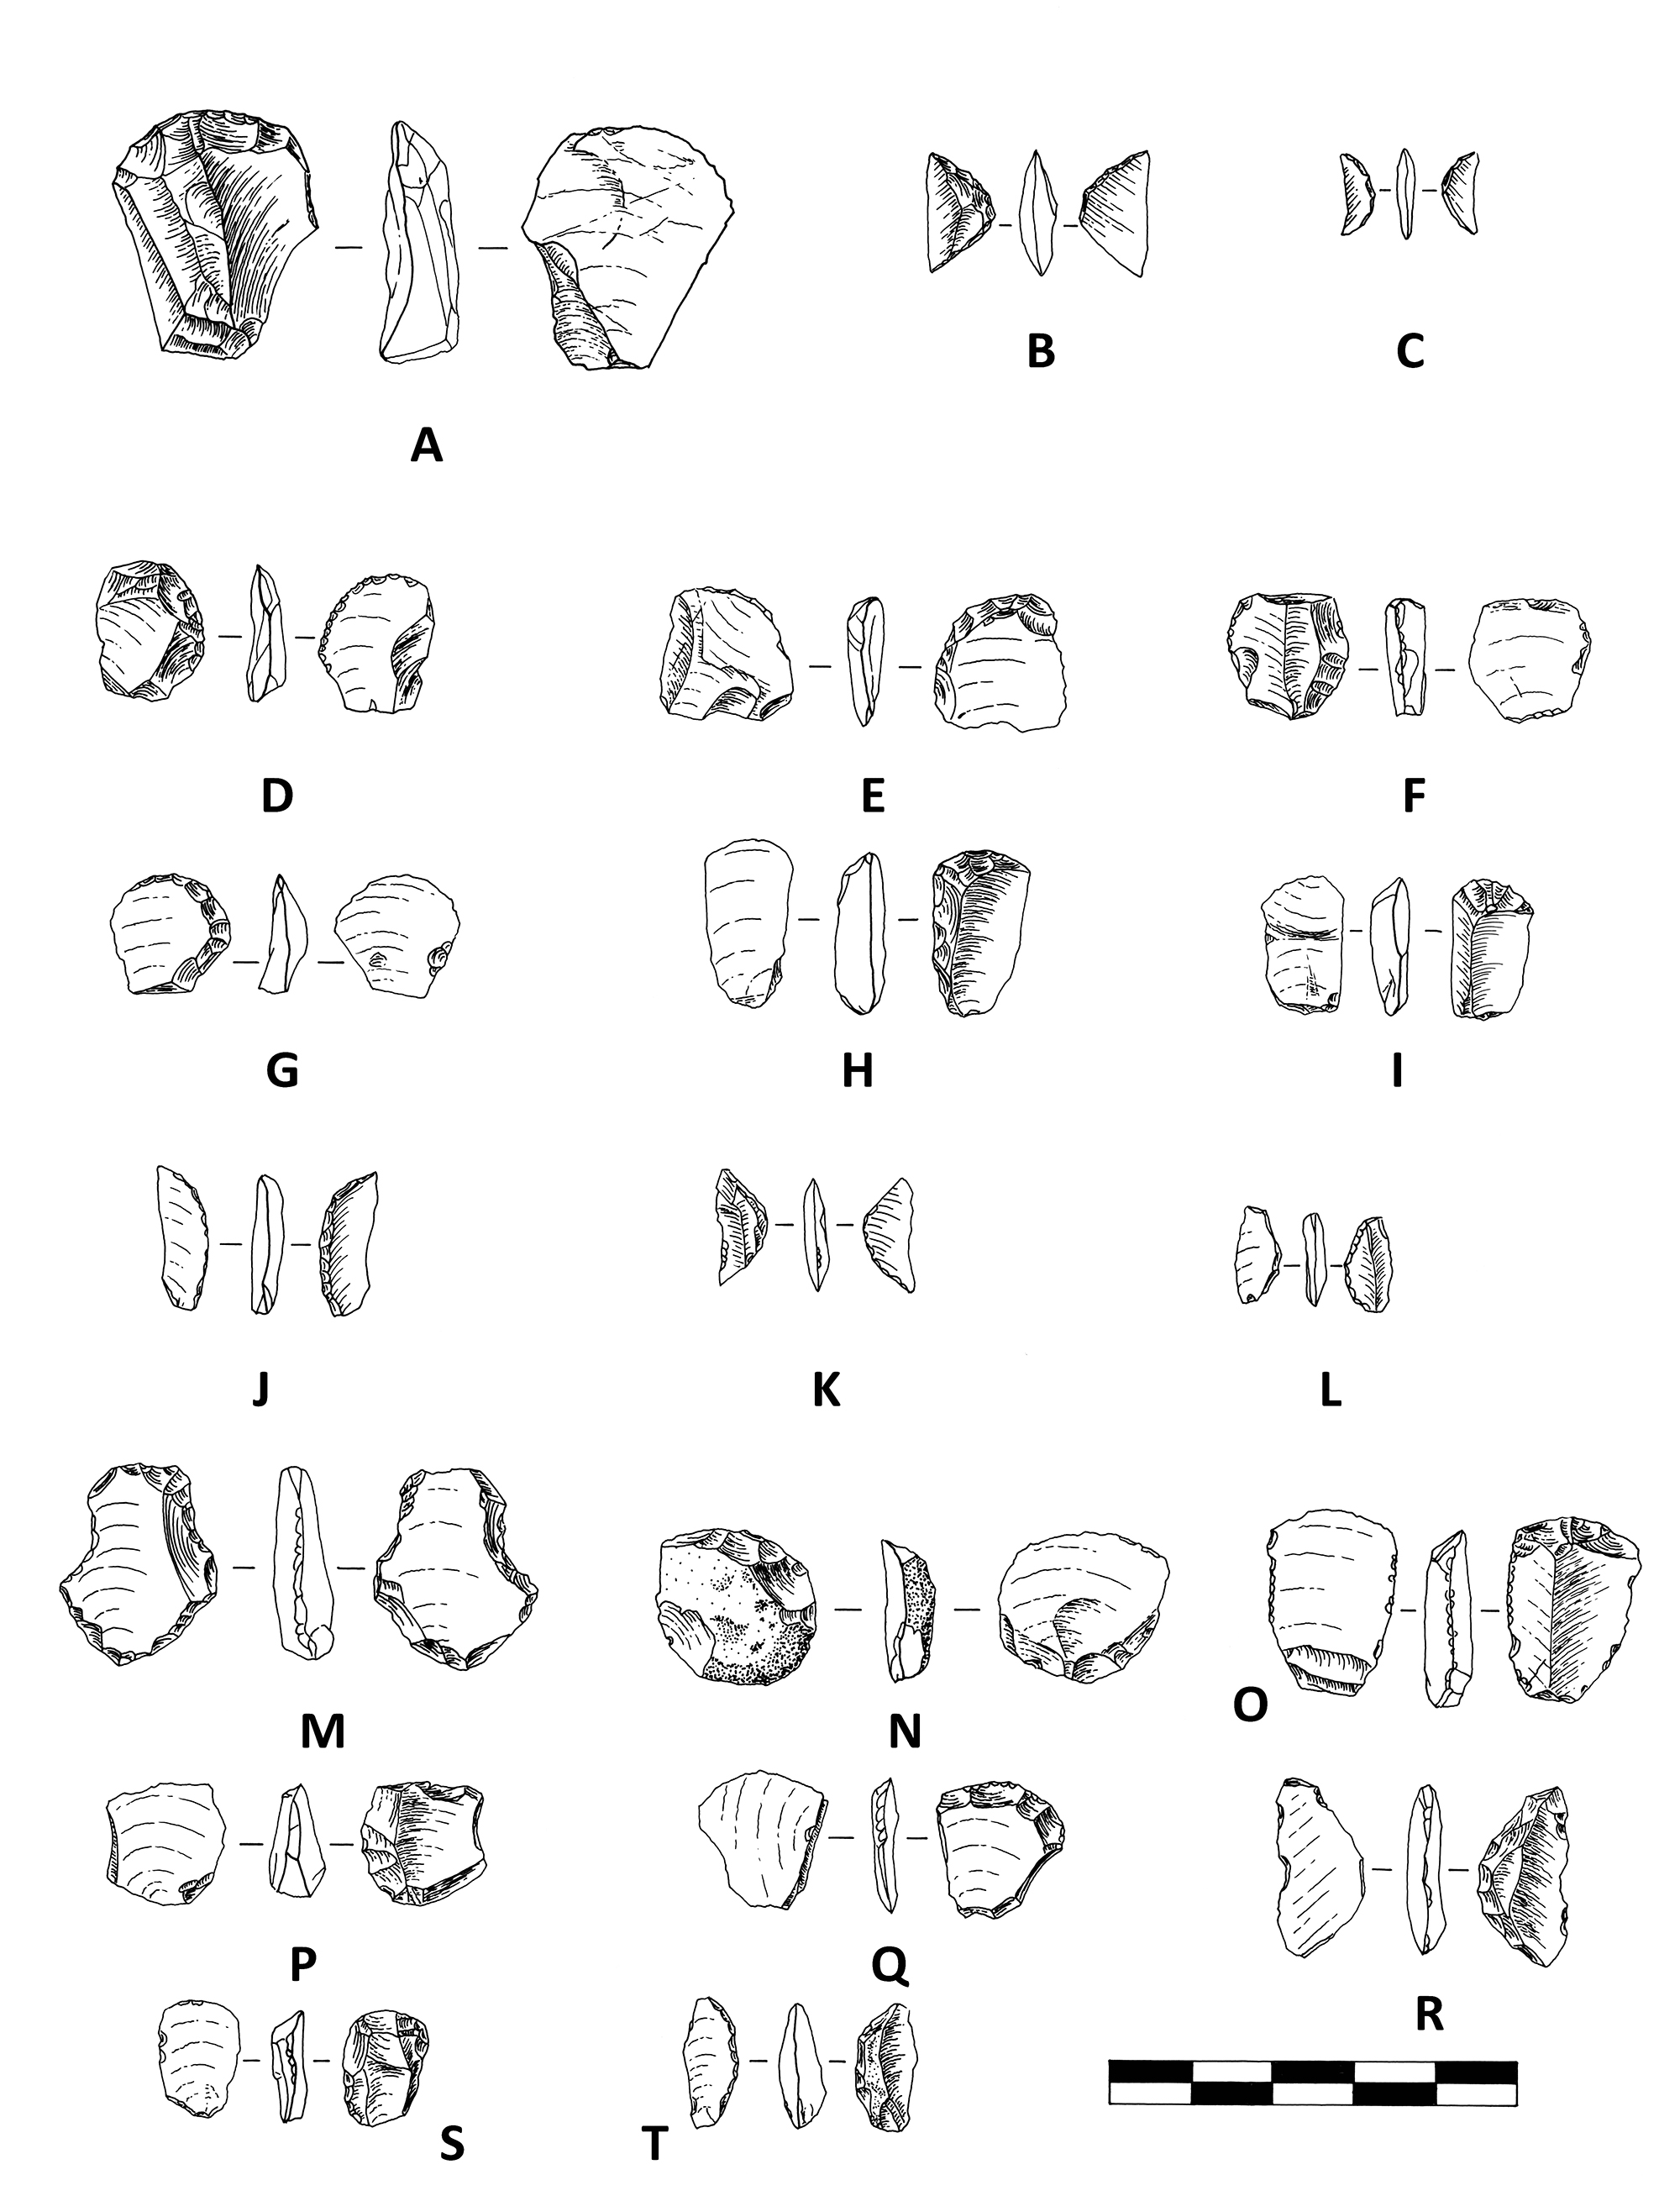
\includegraphics[width=\linewidth]{figures/Forssman-Figure05}
		\caption{Examples of formal tools from Mafunyane: A \& O, medium end scarper; B, C, K \& R, segment; D, F \& S, small side scraper; E, G-I, N, P \& Q, small end scraper; J, L \& T, segmented backed bladelet; and M, adze.}
		\label{fig:Forssman-Figure05}
	\end{figure}
	
		\begin{figure} %Figure 6
			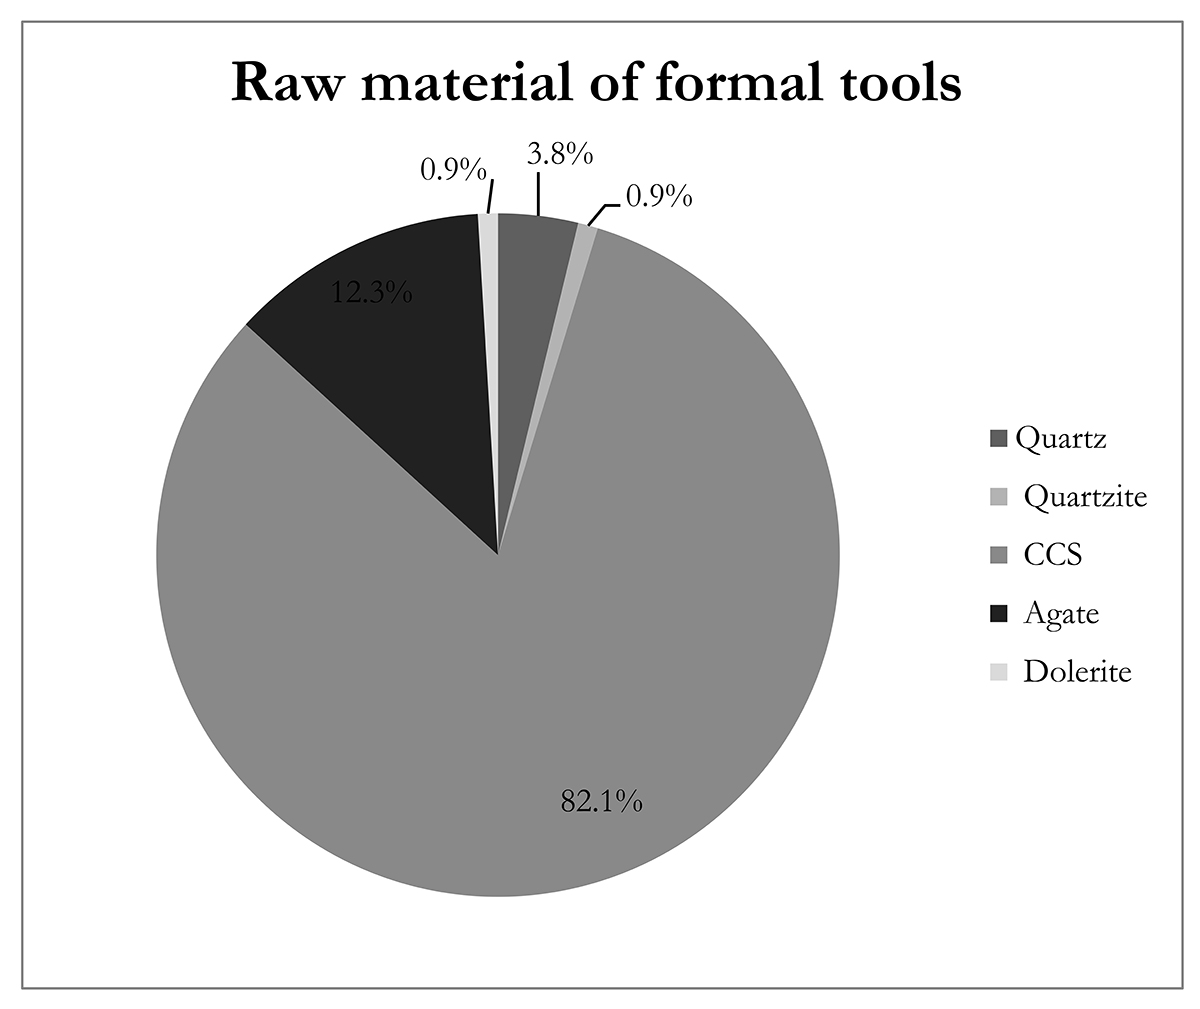
\includegraphics[width=\linewidth]{figures/Forssman-Figure06}
			\caption{Raw material utilisation in the formal tool assemblage.}
			\label{fig:Forssman-Figure06}
		\end{figure}
	
	\begin{figure} %TABLE 3
		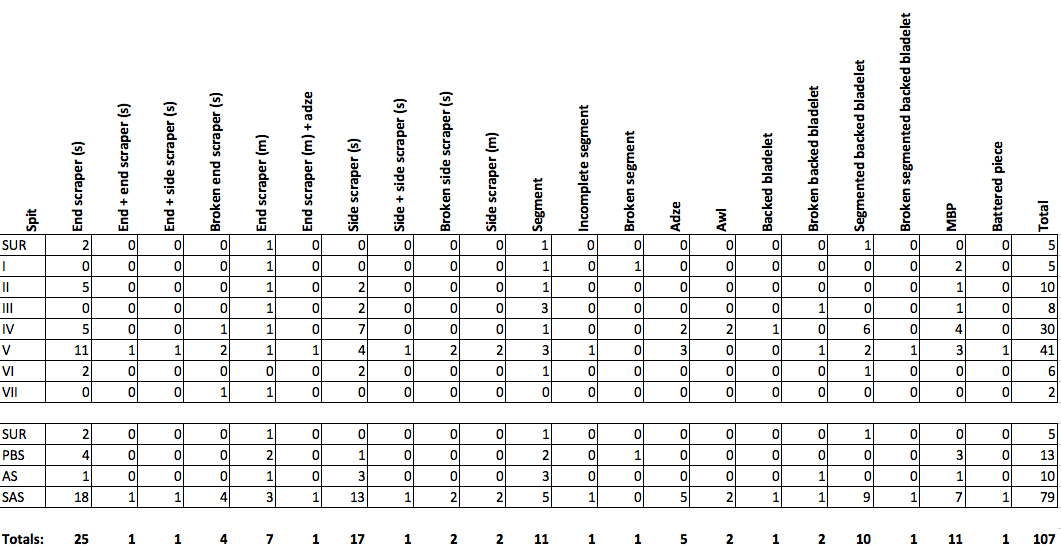
\includegraphics[width=\linewidth]{figures/Forssman-Table03}
		\captionof{table}{Formal tool types and distribution separated by spits and stratigraphic layers. Scrapers marked with s (small), m (medium) and l (large) indicate their size class.}
		\label{fig:Forssman-Table03}
	\end{figure}
   
   The majority of scrapers (n=46) and backed tools (n=18) were found in SAS, the lowermost unit (\cref{fig:Forssman-Table04}). 
  It is also within this stratigraphic unit that the majority of stone tools were found and may have been a period of increased activity at the site, or in the population living at the rockshelter (but no depositional study has been performed). Scraper and backed tool lengths varied between the spits and throughout the deposit. The average scraper length is \SI{16.3}{\milli\meter} 
   while the average length of backed tools is \SI{14.7}{\milli\meter}. 
  It is clear that while scraper lengths vary from the base of the trench to the surface, there is no distinctive pattern, 
   although in general they appear to increase in size across the spits whereas between the stratigraphic units they decrease. Backed tools on the other hand decrease in size between both the spits and stratigraphic units. These findings are consistent with those made by \textcite[31]{Walker_1994}.
   
   	\begin{figure} %TABLE 4
   		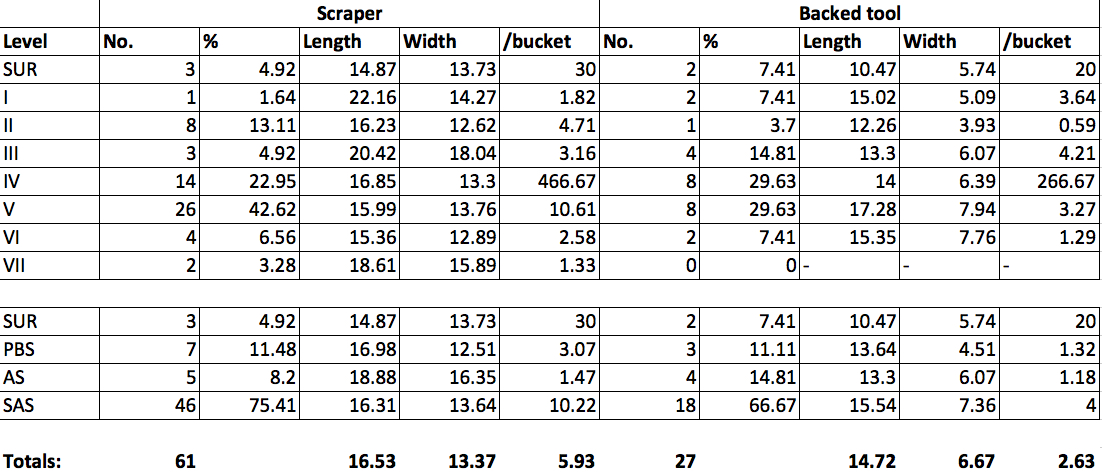
\includegraphics[width=\linewidth]{figures/Forssman-Table04}
   		\captionof{table}{Scraper and backed stone tool distribution and density based on the spits (above) and stratigraphic layers (below).}
   		\centering
   		\label{fig:Forssman-Table04}
   	\end{figure}
   
%\section*{Ceramics}

Ceramics occur from the \IJSRAsection{Ceramics} surface to Spit VI but generally in low densities (on average 3/bucket; \cref{fig:Forssman-Figure07}). 
A total of 31 sherds were recovered with most being undiagnostic or plain 
(n=28; \SI{90.3}{\percent}). 
Two decorated (\SI{6.5}{\percent}) and one plain rim (\SI{3.2}{\percent}) were also found as well as a decorated rim on the surface outside the excavation but still within the rockshelter (\cref{fig:Forssman-Figure08}). 
Unfortunately, the decorated sherds are small and difficult to place within a ceramic facies with any certainty. However, based on the incised decorations and their location in the neck it is possible that they are from the K2 facies.\footnote{\AD 1000 to 1220; ceramic identification Antonites pers. comm. 2015} 
This designation is supported by the Leopard’s Kopje ceramics (\AD 1000 to 1300; K2 is a sub-group within the Leopard’s Kopje branch) identified by \textcite{Walker_1994}. 
If accurate, the ceramic facies represented at the site overlaps with a large portion of the radiocarbon dates from \AD 941 to 1265.

	\begin{figure} %Figure 7
		\includegraphics[width=\linewidth]{figures/Forssman-Figure07}
		\caption{Ceramic distribution showing a peak in Spits II and III.}
		\label{fig:Forssman-Figure07}
	\end{figure}
	
		\begin{figure} %Figure 8
			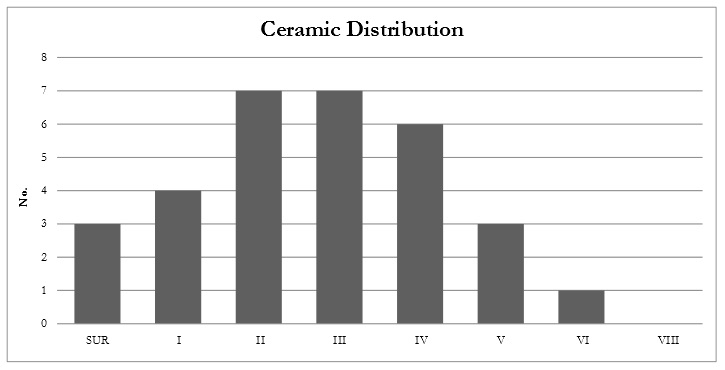
\includegraphics[width=\linewidth]{figures/Forssman-Figure08}
			\caption{Decorated ceramics from Mafunyane too small to identify with certainty but might be K2}
			\label{fig:Forssman-Figure08}
		\end{figure}

%\section*{Shell, Bone, Glass, and Metal Beads}

A total of 54 \IJSRAsection{Shell, Bone, Glass, and Metal Beads} beads were recovered from the excavation, of which 41 are made from ostrich eggshell (\SI{75.9}{\percent}), 
six from bone (\SI{11.1}{\percent}), 
three each from land snail and glass (\SI{5.6}{\percent}) and one from metal (\SI{1.9}{\percent}; 0.1/bucket; \cref{fig:Forssman-Table05}). Ostrich eggshell beads are divided into four categories \parencite[after][]{Orton_2008}: 
complete (\SI{40}{\percent}), broken (\SI{15}{\percent}), 
incomplete/preform (\SI{15}{\percent}) and broken preform (\SI{30}{\percent}). 
All ostrich eggshell beads were measured and the complete specimens have an average length of 
\SI{3.7}{\milli\meter} and a width of \SI{3.6}{\milli\meter}. 
Of the complete beads, there are 14 small beads (< \SI{5}{\milli\meter}), 
typically associated with foragers \parencite[c.f.][]{Orton_2014}, and four medium beads (\SIrange{5}{6}{\milli\meter}). 
In both the spit and stratigraphic units the average length of beads decreased from Spit V to the surface (no complete beads were found in Spits VI and VII). 
Broken and preform ostrich eggshell bead lengths displayed no pattern but broken preforms decrease in length from the base of the trench; it might indicate that a preference for smaller beads occurred in the more recent deposits but if so one would expect the same pattern in the previous two categories. The different bead variations appear throughout the trench, barring in Spit VII,
 and no pattern is discernible (\cref{fig:Forssman-Figure09,fig:Forssman-Figure10}). 
 The presence of beads in various states of manufacture indicate that during Mafunyane’s occupation ostrich eggshell bead processing was occurring at the site, 
 and if the beads \textcite{Walker_1994} identified are included (n=67) it is possible that the manufacturing operation was either of a considerable scale or took place over a short intense period of production. 
 
    	\begin{figure} %TABLE 5
    		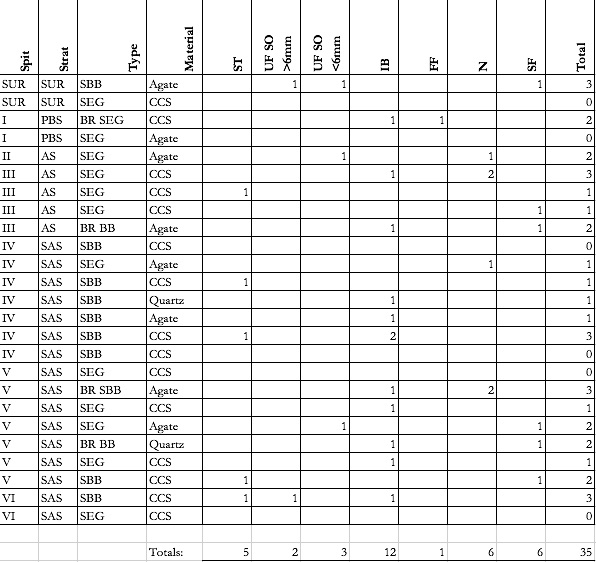
\includegraphics[width=\linewidth]{figures/Forssman-Table05}
    		\captionof{table}{The distribution and density of bead types from Mafunyane’s spits (above) and stratigraphic units (below).}
    		\centering
    		\label{fig:Forssman-Table05}
    	\end{figure}
 
 	\begin{figure} %Figure 9
 		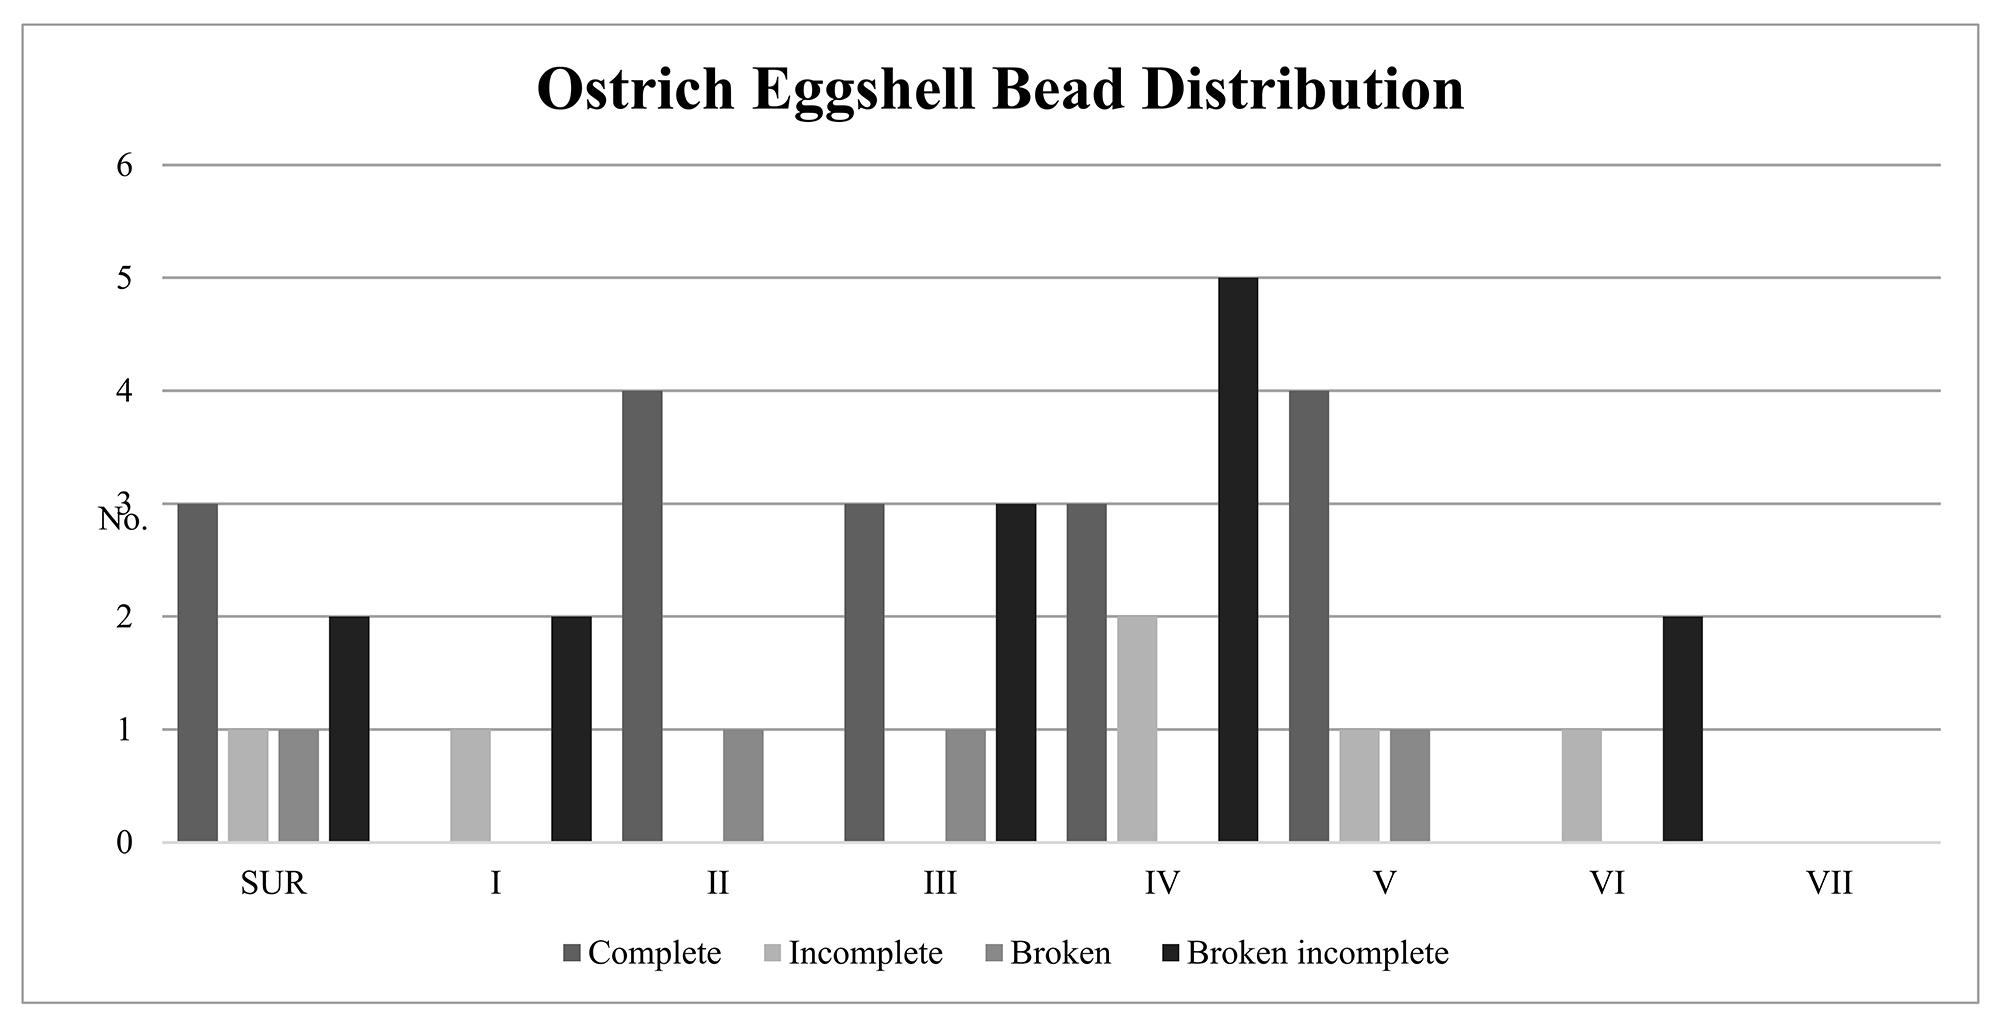
\includegraphics[width=\linewidth]{figures/Forssman-Figure09}
 		\caption{The distribution of the different ostrich eggshell bead forms is inconsistent but their presence suggests bead manufacturing was occurring at Mafunyane.}
 		\label{fig:Forssman-Figure09}
 	\end{figure}
 	
 	\begin{figure} %Figure 10
 		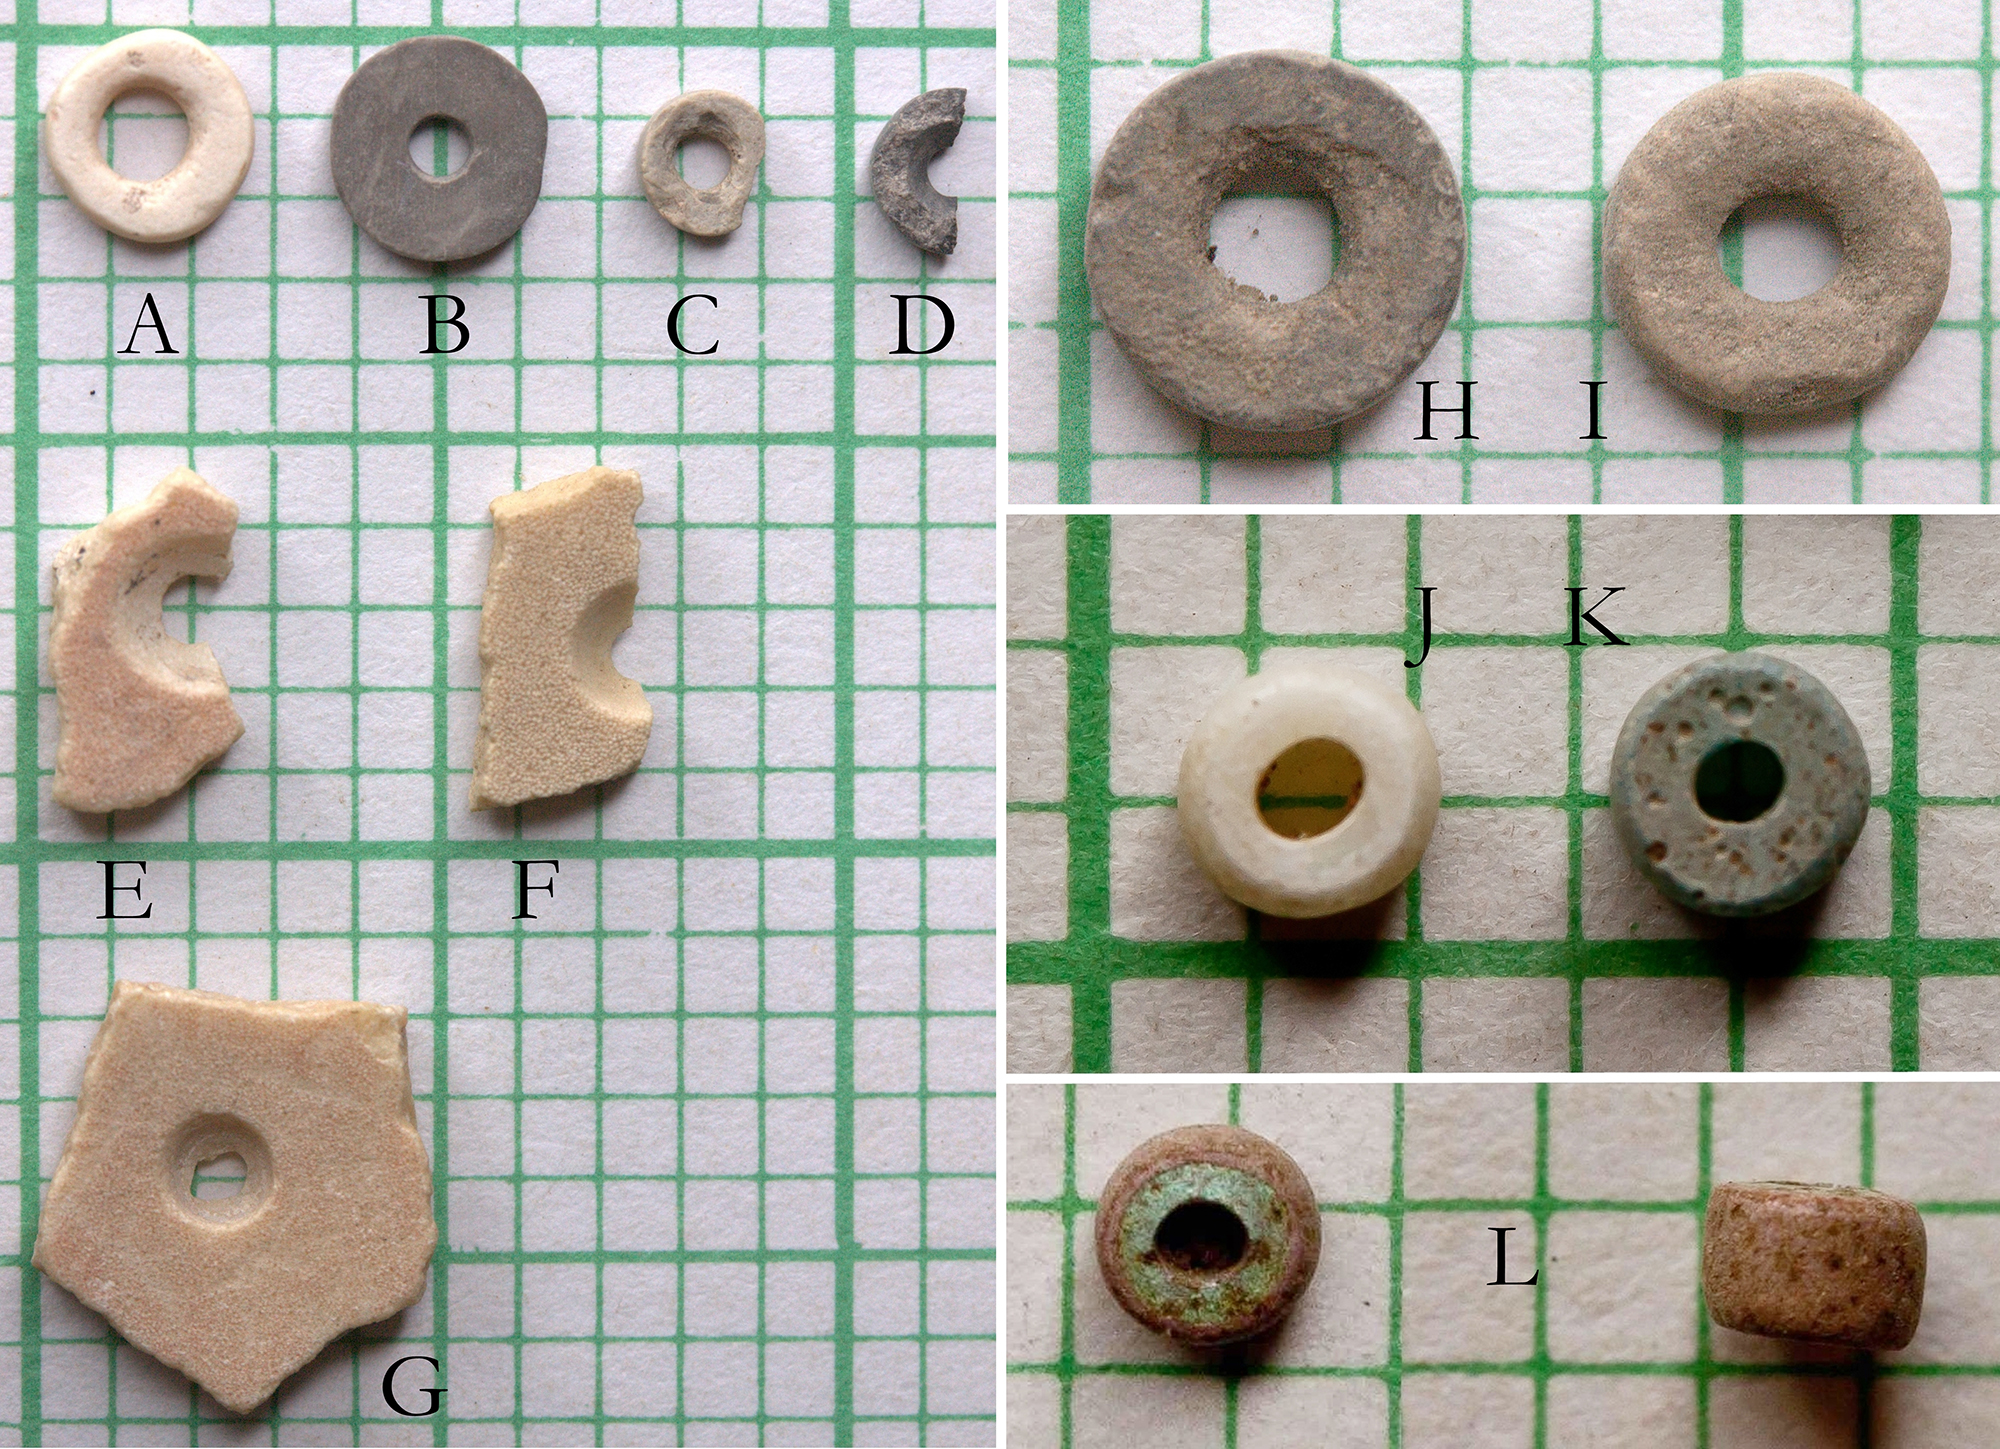
\includegraphics[width=\linewidth]{figures/Forssman-Figure10}
 		\caption{Ostrich eggshell and glass beads: A-C, H \& I, complete; D, broken complete; E-F, broken preform; and G, preform; J \& K, European possibly dating from the eighteenth century; and L, European red-on-green (\AD 1600 to 1800s; scale \SI{2}{\milli\meter}).}
 		\label{fig:Forssman-Figure10}
 	\end{figure}
 
 
 The glass beads are European, two possibly dating to the eighteenth and nineteenth centuries (\cref{fig:Forssman-Figure10}J \& K) 
 and one post-dating the seventeenth century (\cref{fig:Forssman-Figure10}L). 
 It is possible that all were introduced after foragers abandoned the rockshelter. 
 Each glass bead was given a Munsell value using the Munsell colour chart for glass beads: 
 \cref{fig:Forssman-Figure10}J is white (N9) and \cref{fig:Forssman-Figure10}K is medium blue (5.0B 4/6) 
 and each is opaque-translucent 
 \parencite[slight glow of light along edges;][70]{Wood_2011}. 
 \Cref{fig:Forssman-Figure10}L is opaque with an outer colour of orchid mist (2.5RP 7/4) and an inner colour of light turquoise (10.0GB 7/4).  
 \textcite{Walker_1994} found six glass beads and all but one were in the top unit - he did not place them into a typology or determine their Munsell value. 
 Only a single wound metal bead was recovered from Spit I but \textcite{Walker_1994} found a total of 16 at the site.

%\section*{Other Finds}

There are 14 pieces \IJSRAsection{Other Finds} of worked metal, including the metal bead, between Spits I and IV (\cref{fig:Forssman-Figure11}). \textcite{Walker_1994} 
suggested that the metal he found was copper and it appears consistent with copper artefacts in the
\citeauthor{Miller_2001} \parentext{\citeyear{Miller_2001}, \citeyear{Miller_2002}}
% \textcites{Miller_2001}{Miller_2002} 
reports from K2 and around Mapungubwe. 
To confirm this, an X-ray fluorescence analyses was performed on three artefacts. 
It was found that \cref{fig:Forssman-Figure12}A and C were copper alloys (C194HiCu and C197HiCu) with all three samples relatively pure in copper (> \SI{98.8}{\percent}; \cref{fig:Forssman-Figure12,fig:Forssman-Table06}). 
Metal prills \parencite[see][]{Miller_2001}, 
likely copper but not tested, occurred in various densities between the surface and Spit V, totalling \SI{134.2}{\gram}, 
but were concentrated between Spits II and V. Also found at these depths were the two slag pieces (Spits III and IV). 
In addition, what appears to be a fragment of a tuyère was found in Spit IV and is an item used in both smithing and smelting practices \parencites{Miller_2001}{Miller_2002}. 
Lastly, a possible clay figurine fragment was also found in Spit II and appears to include a portion of the back leg, the stomach and the rump of a mammal.

	\begin{figure} %Figure 11
		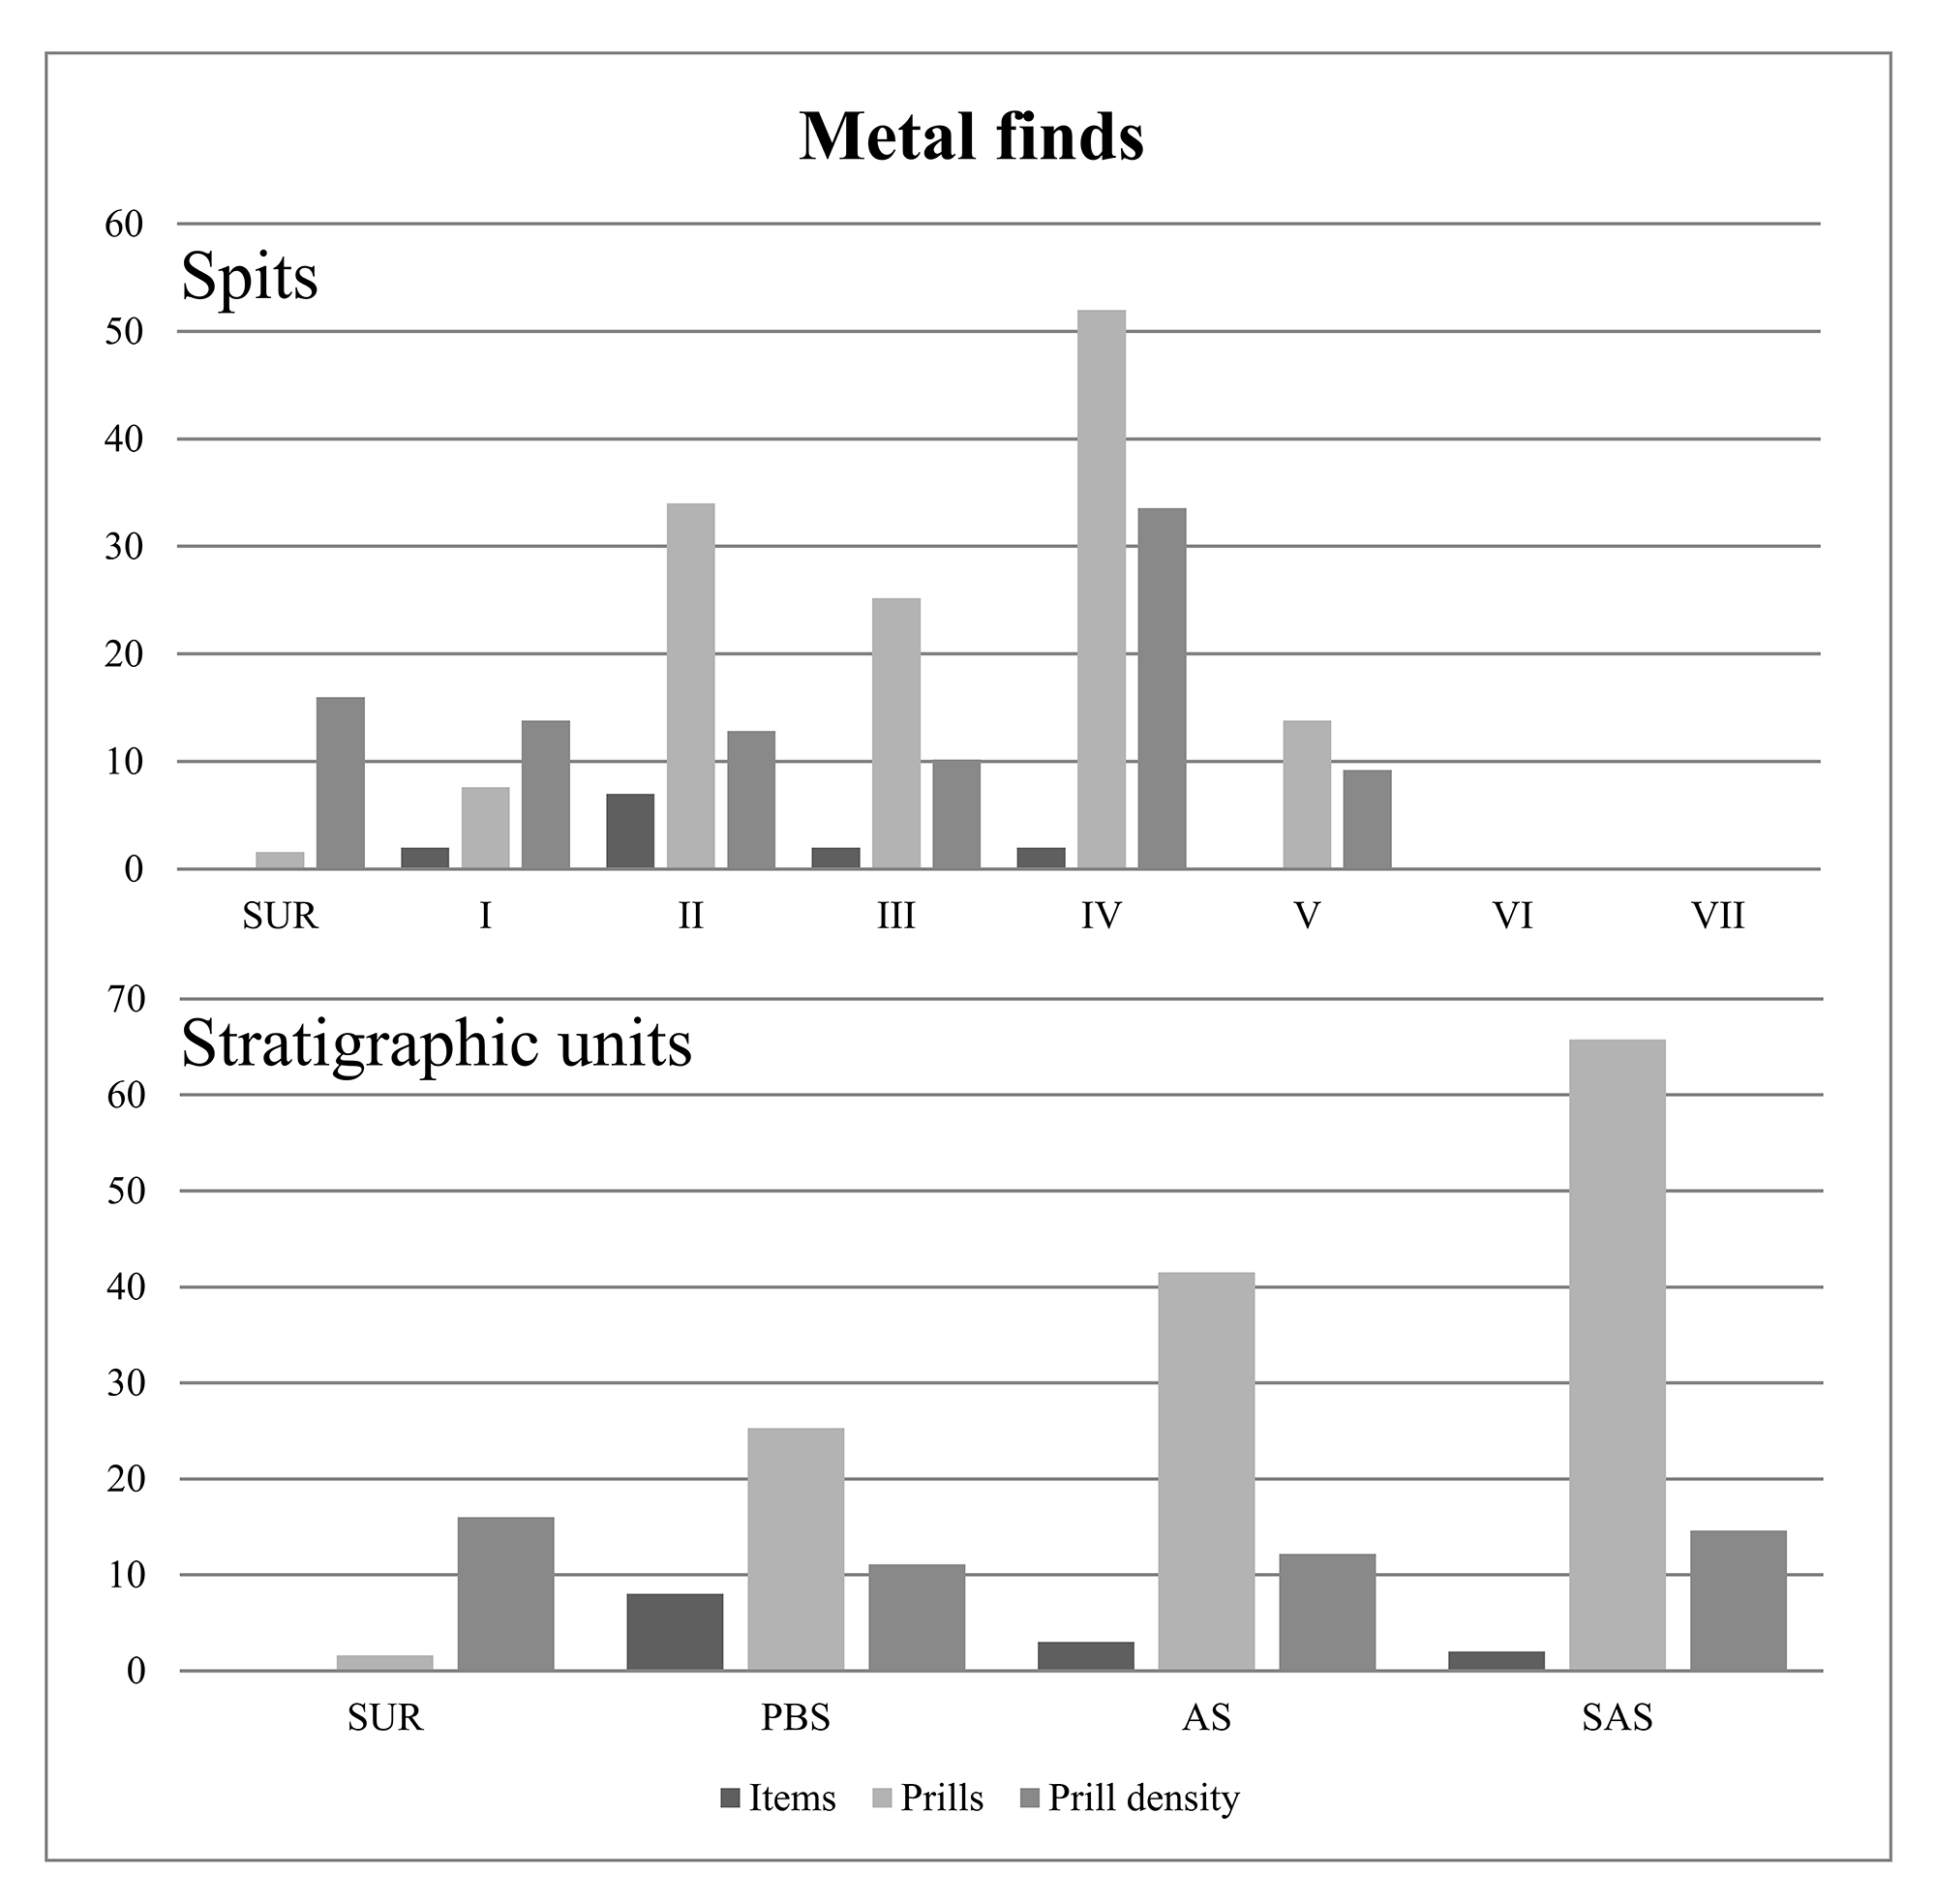
\includegraphics[width=\linewidth]{figures/Forssman-Figure11}
		\caption{The distribution of metal items, prills and the density of metal prills; metal first appears in Spit V, part of SAS.}
		\label{fig:Forssman-Figure11}
	\end{figure}

	\begin{figure} %Figure 12
		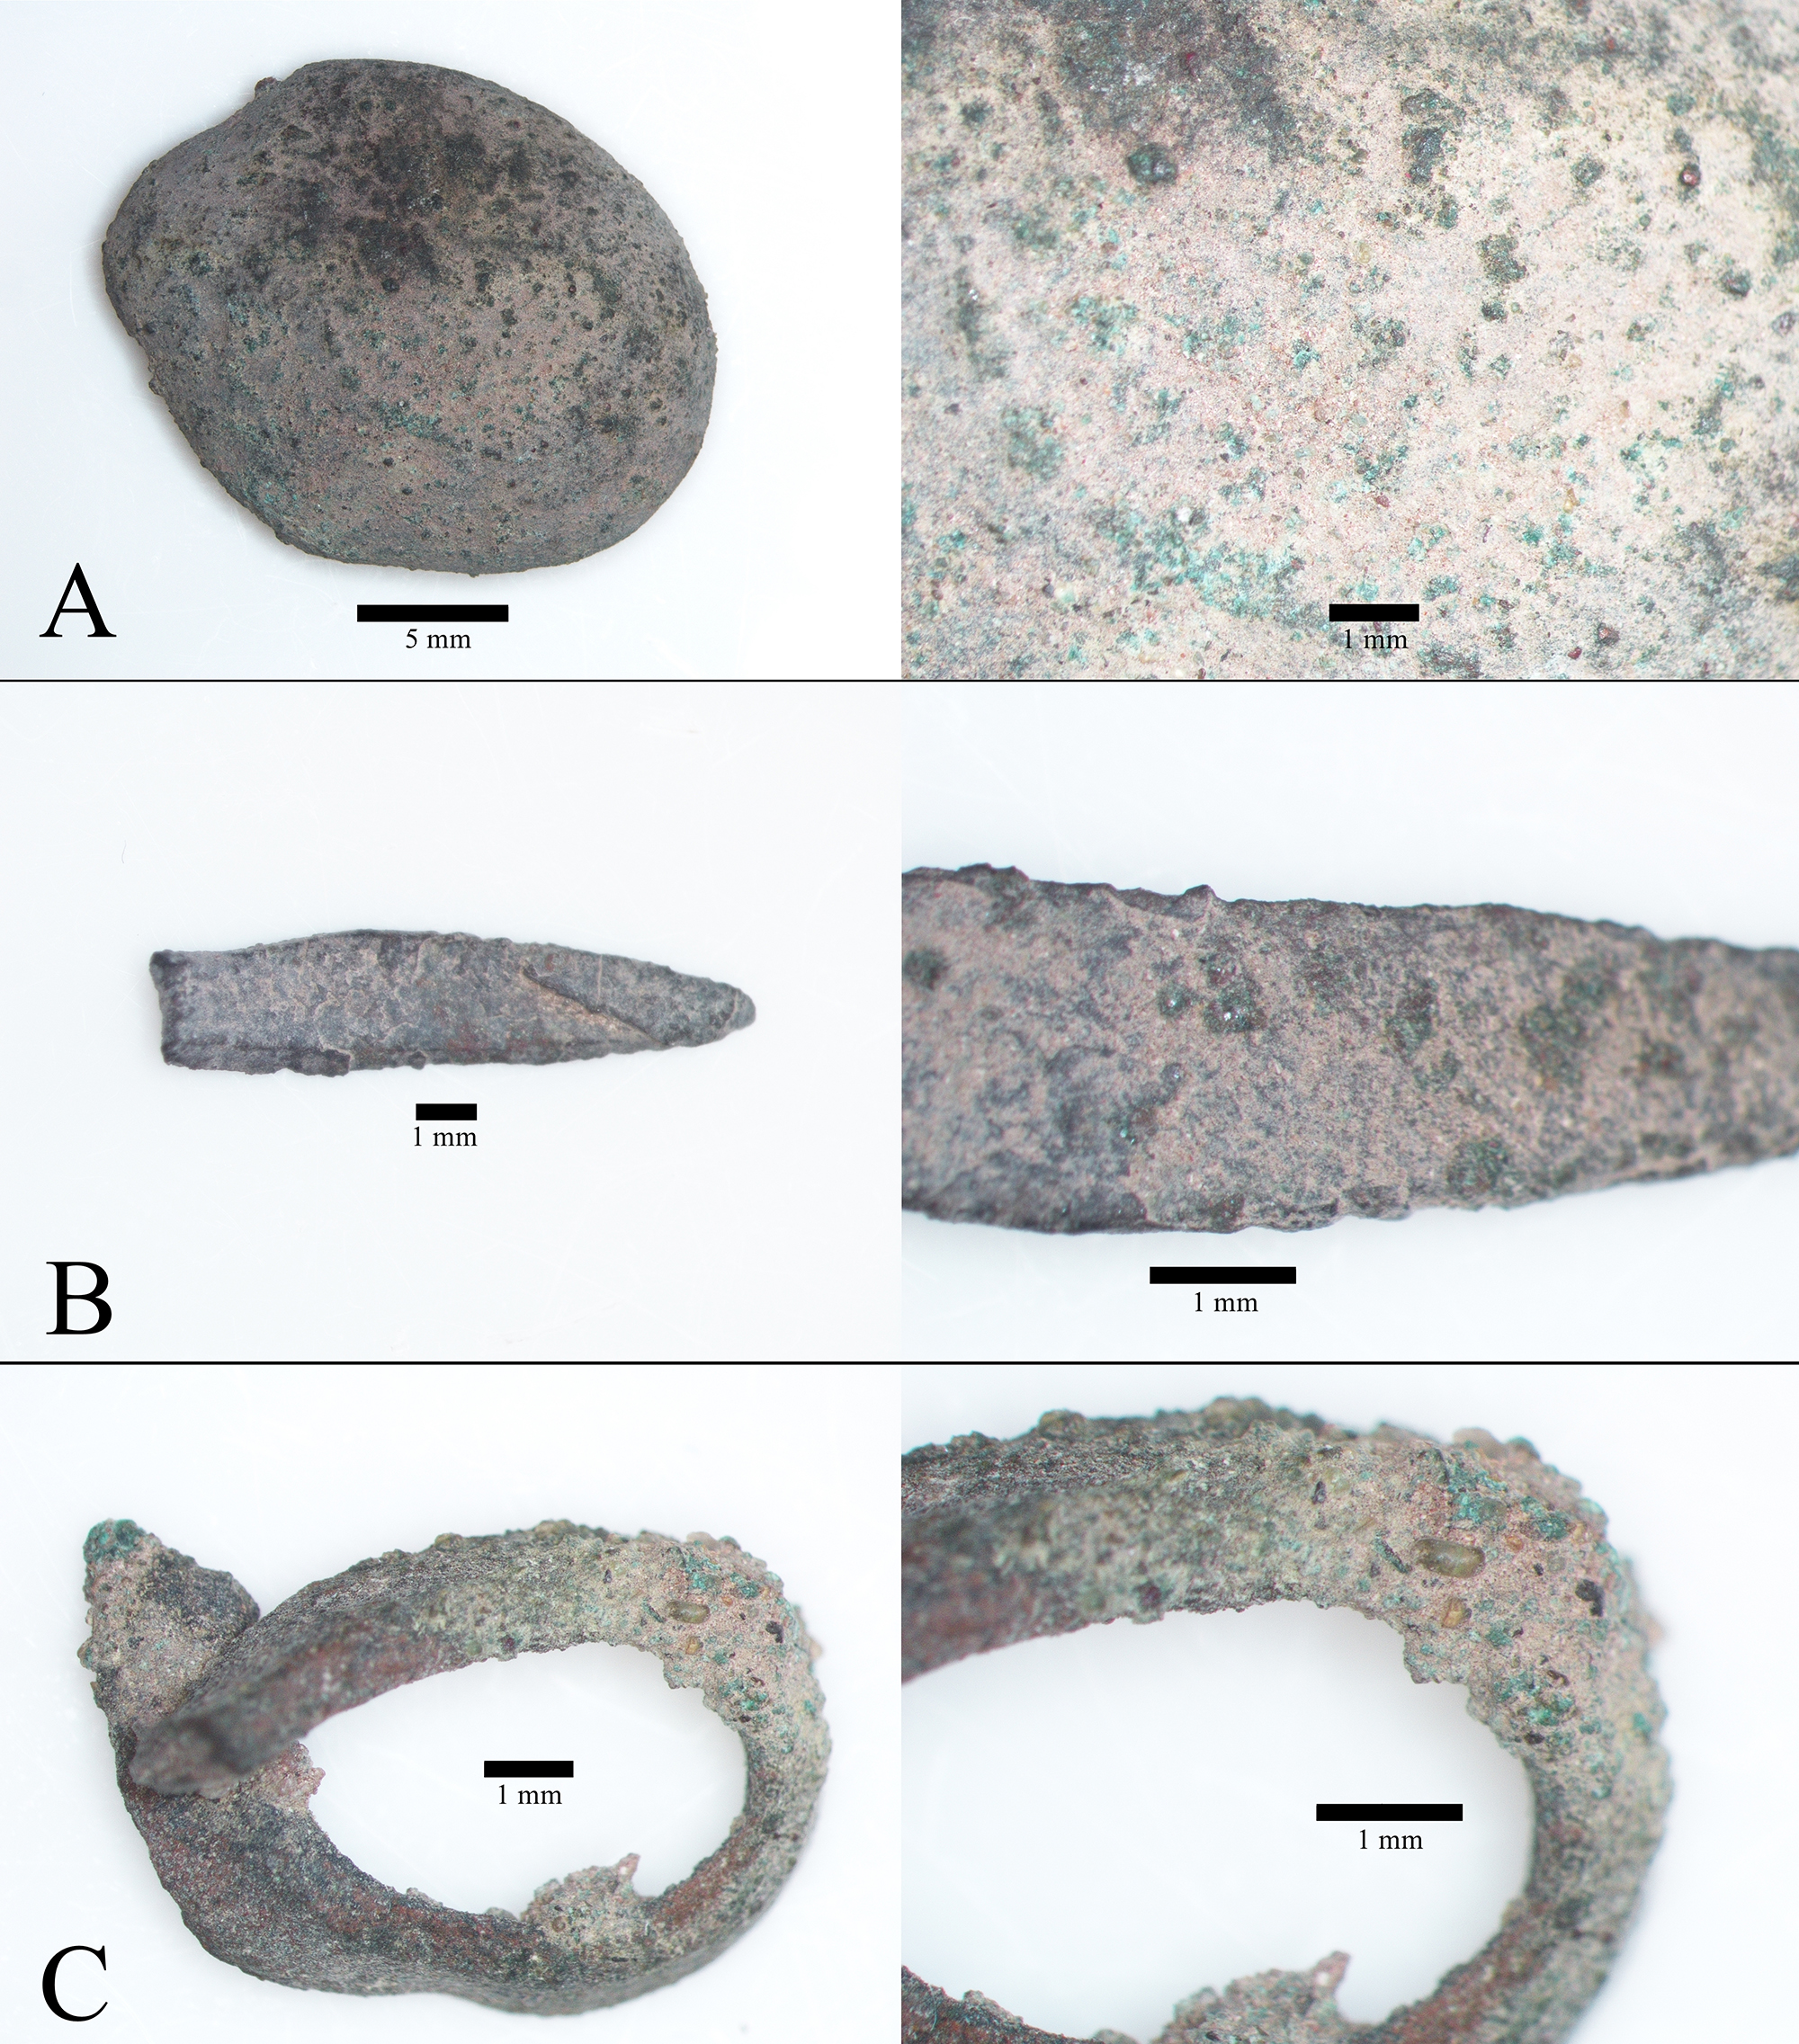
\includegraphics[width=\linewidth]{figures/Forssman-Figure12}
		\caption{The three samples submitted for XRF analysis (A – C). In each case the right imaged is a magnified portion of the sample; note the cuprous green and red patination on each specimen.}
		\label{fig:Forssman-Figure12}
	\end{figure}

    	\begin{figure} %TABLE 6
    		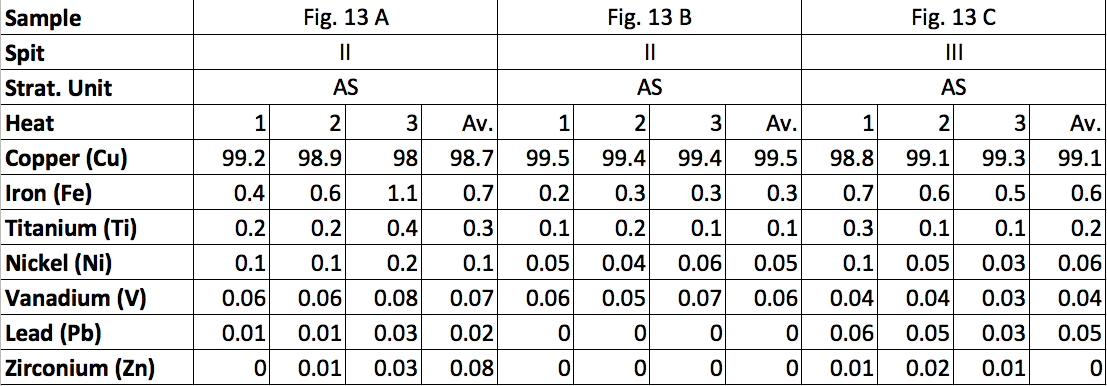
\includegraphics[width=\linewidth]{figures/Forssman-Table06}
    		\captionof{table}{XRF analysis results from samples shown in Fig 12: sample numbers in \% and Av. is the average of the three heats. Note that copper dominates and no other metal is > \SI{1}{\percent}.}
    		\centering
    		\label{fig:Forssman-Table06}
    	\end{figure}

%\section*{Fauna}
The combined \IJSRAsection{Fauna} mass of the faunal remains is \SI{845.8}{\gram} (\SI{82.3}{\gram}/bucket) and the highest number of identifiable specimens (NISP) 
and density of non-identified remains (\SI{300.1}{\gram}/ bucket; \cref{fig:Forssman-Table07}) occurs in Spits IV and V. 
The most frequent faunal specimen at the site is tortoise (n=50), which was mostly identified from carapace remains, followed by lizard (n=15) and small bovids (n=4). Fish remains were identified in both this and the \textcite{Walker_1994} study. 
Of interest is the presence of various items associated with farming communities but the total lack of domesticates, 
also noted by \textcite{Walker_1994}. 
It could indicate that farmers used the site for a specific and possibly non-residential purpose, that they did not have access to livestock, 
or that the food remains were deposited elsewhere. 
As will be argued, the former explanation seems most likely.

    	\begin{figure} %TABLE 7
    		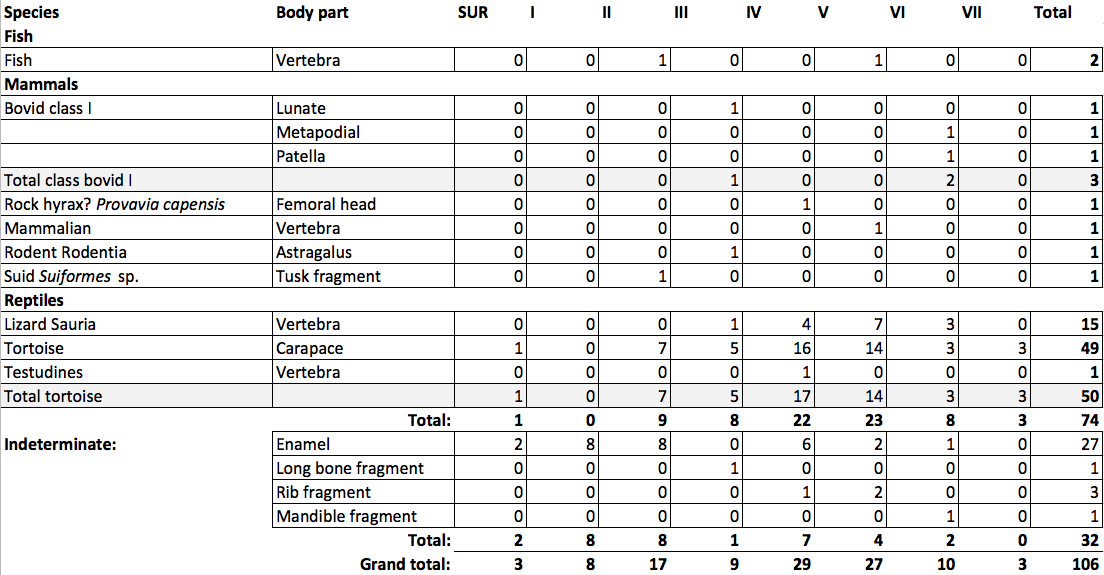
\includegraphics[width=\linewidth]{figures/Forssman-Table07}
    		\captionof{table}{The NISPs from the Mafunyane Shelter demonstrate a noticeable lack of domesticates.}
    		\centering
    		\label{fig:Forssman-Table07}
    	\end{figure}

%\section*{Rock Markings}

Grooves, cupules and \IJSRAsection{Rock Markings} rock art were found in and around the rockshelter. Grooves were found inside on a large rock (n=21) with an additional cluster of more than 20 identified on an exposed rock to the west of the site. 
Nine cupules were located all occurring inside the rockshelter (\cref{fig:Forssman-Figure13}). 
The presence of metal items and ostrich eggshell beads in various stages of production might indicate that 
the grooves and cupules were used in related activities, but this cannot be said with certainty. 
Red and black monochrome rock paintings were also recorded at the site but are unfortunately heavily faded (\cref{fig:Forssman-Figure14}).
In the main portion of the rockshelter, where the excavation was performed, a black giraffe and sable or roan antelope were identified, and painted at the eastern edge are a procession of four humans, two of which appear to be females, and an indeterminate animal. 

	\begin{figure} %Figure 13
		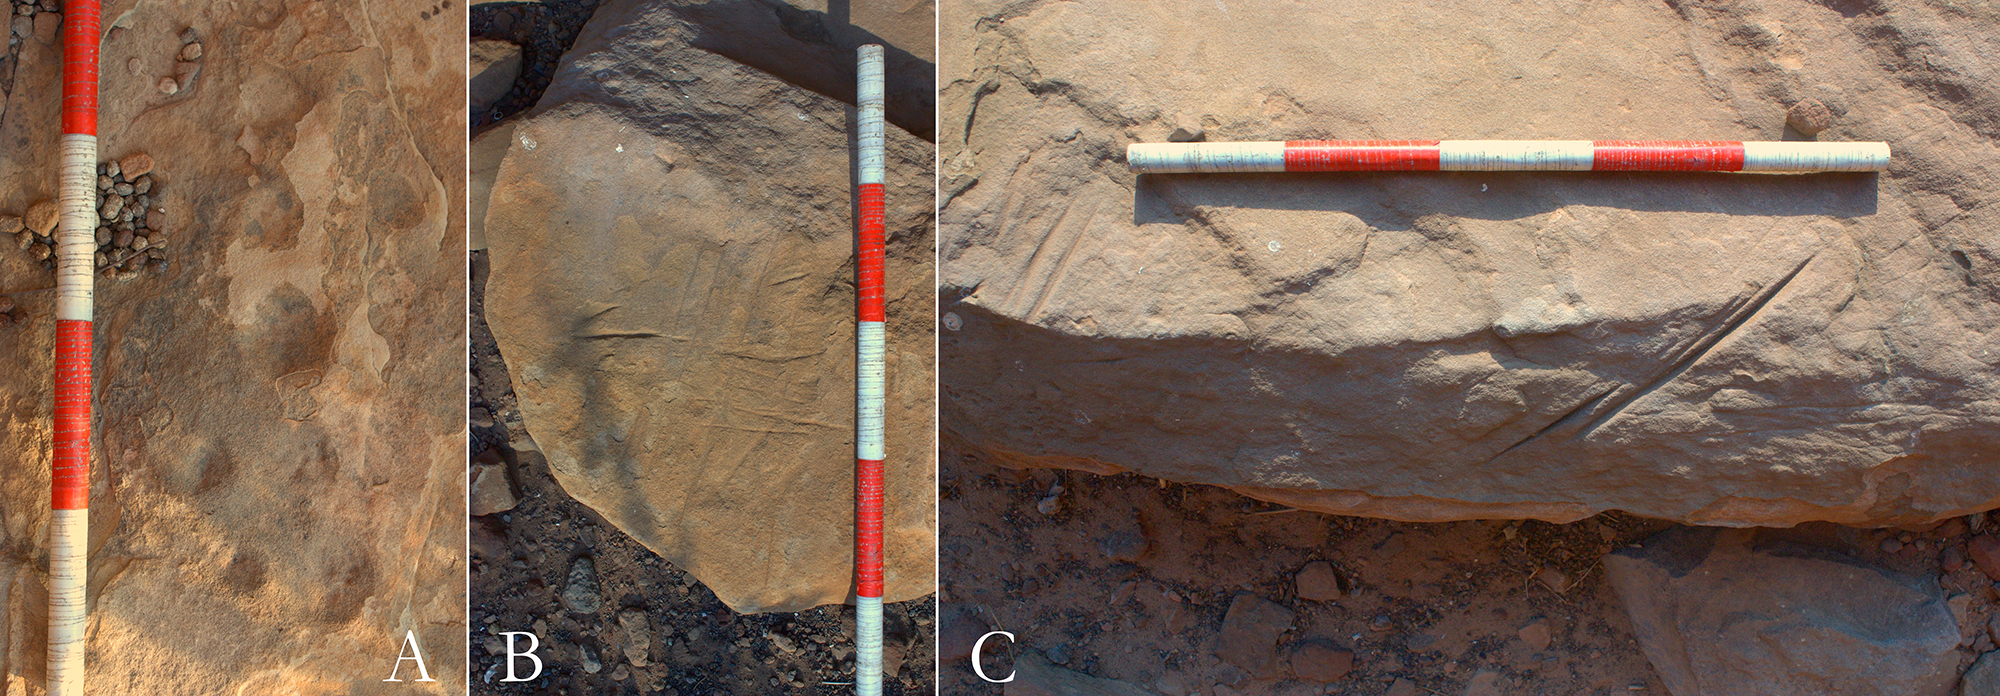
\includegraphics[width=\linewidth]{figures/Forssman-Figure13}
		\caption{Cupules (A) and grinding grooves (B \& C) from inside the rockshelter.}
		\label{fig:Forssman-Figure13}
	\end{figure}
	
	\begin{figure} %Figure 14
		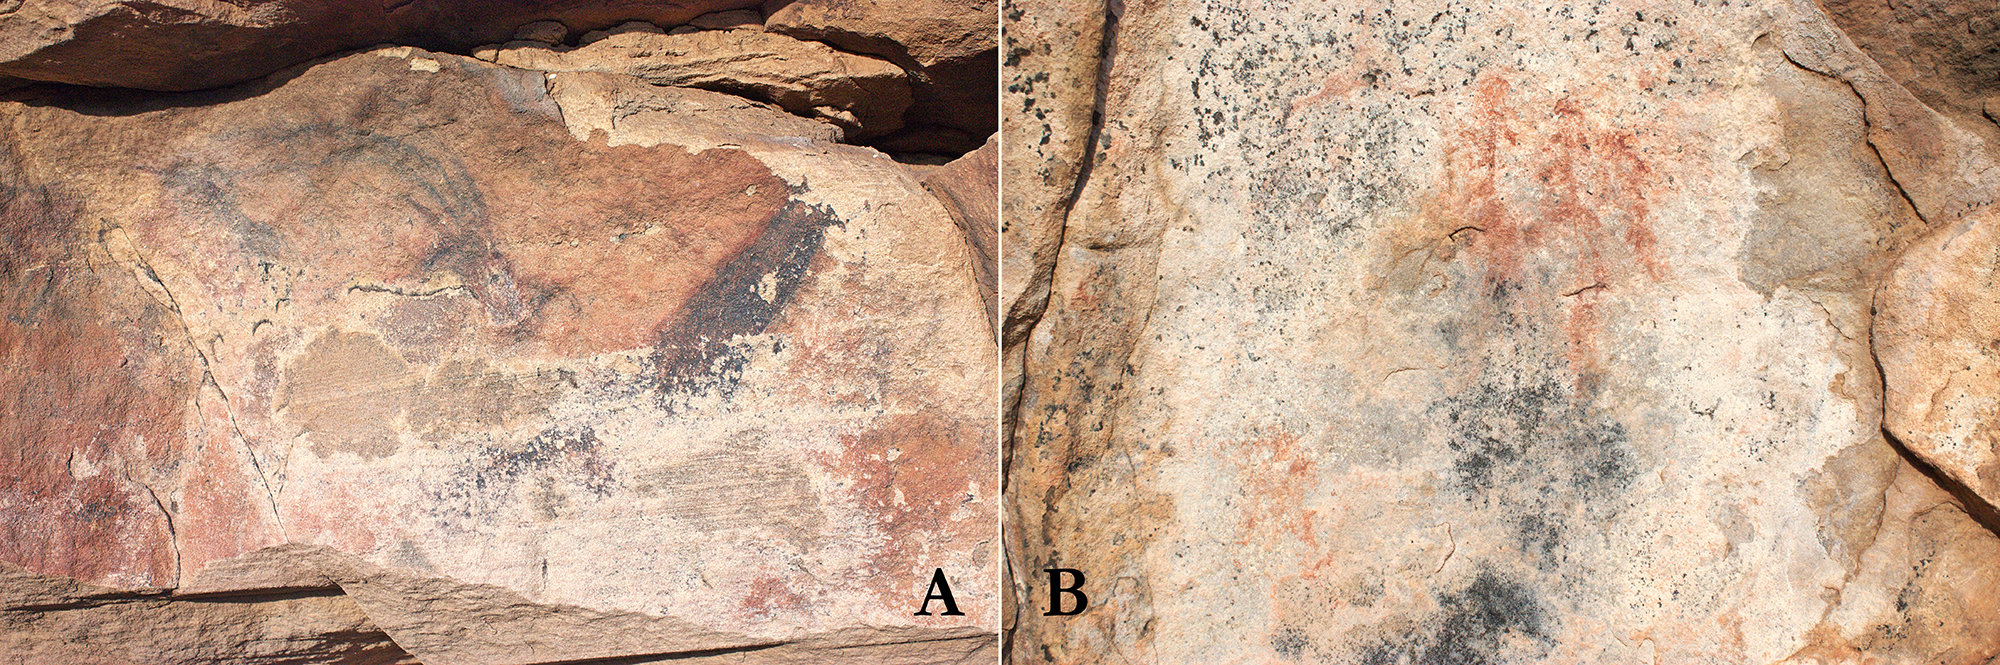
\includegraphics[width=\linewidth]{figures/Forssman-Figure14}
		\caption{Possible sable or roan antelope and giraffe (A) and a procession of four humans, two identified as female, and an indeterminate antelope (B).}
		\label{fig:Forssman-Figure14}
	\end{figure}

%\section*{Discussion and Conclusions}

Mafunyane contributes to the \IJSRAsection{Discussion and Conclusions} growing body of work exploring the local LSA sequence. 
Until recently, most of this research was performed in South Africa and focussed primarily at large rockshelters. 
While the work of \textcite{Hall_2000} and \textcites{vanDoornum_2007}{vanDoornum_2008}{vanDoornum_2014} established a tight chronological record of the region’s LSA record as well as shifts in forager material culture, it is unlikely that by asking the same questions and excavating the same sites types we are going to further develop their findings. However, revising our research agendas and expanding our approach might lead to an improved regional understanding of LSA dynamics. Achieving this includes working in Botswana and Zimbabwe. Mafunyane, in part, contributes to these renewed goals. 

It would be remiss to not first consider the possibility of post-depositional mixing given the inverted radiocarbon dates. If this has occurred, it might explain the overturned results. The occurrence of metal-working related activities (discussed below) may have altered the deposit inadvertently. The extent of this cannot be fully assessed until further analysis is performed, but the lack of ceramics and metal in the basal level might suggest that if mixing occurred, it did not affect the entire assemblage equally. Nevertheless, the dated range is from \AD 941 to 1235, a roughly 300 year period, and if accurately identified the diagnostic ceramics appear to fall within this phase. To some extent supporting this is the dominance of scrapers in all of the stratigraphic levels, typical of contact period LSA assemblages. Since it appears that the site was occupied over a short period of time, mixing, therefore, does not preclude the possibility of interpreting the site’s use by foragers and metal-working people. However, the relationship between the site’s occupants is unknown because the exact timing of their use within the site’s occupation phase cannot be established. 

The LSA material recovered from Mafunyane is similar to what has been found at other locally excavated sites. Namely, it is dominated by CCS materials and has a variety of formal tools. The large amount of stone tools is interesting and there is a far greater density of them than at Balerno Main Shelter, 
a local aggregation site \parencite{vanDoornum_2008}. Perhaps contributing to this is evidence of primary manufacturing at the site, suggested by the large amount of stone chips and cores. The site is located near to the Limpopo River and a seasonal stream from which cobbles could easily have been sourced. The formal tool assemblage is diverse, 
which may suggest that a variety of activities took place, but it is, as mentioned earlier, dominated by scrapers. Scraper lengths vary throughout the deposit, changing inconsistently between both the spits and stratigraphic units, whereas backed tools decrease in length into the upper levels. The inconsistent change in scraper length does not necessarily indicate mixing because the site was occupied over a short period of time and it might suggest that scraper length was not an important consideration in tool production during this period. Lastly, 
the faunal record is relatively small. This could relate to spatial dynamics or behaviour activities at the site influencing discard patterns or it might suggest Mafunyane was occupied by a small group of foragers. Represented in the faunal record is a variety of small mammals (mostly trappable), some reptiles and fish and an absence of larger animals and domesticates. In summary, there is evidence to suggest that the site was a major living camp, as \textcite{Walker_1994} concluded, but the limited faunal evidence found in both excavations may suggest otherwise.

It is difficult to interpret the farmer presence at the site because there is little evidence indicating their use or occupation. No domesticates or homestead features such as grainbin foundations, hut remains, middens or a kraal were recorded and the ceramics could easily have been acquired by foragers through trade. However, in the ashy deposit were metal prills, found between the surface and Spit VI, along with metal tools and a tuyère fragment. \textcite{Walker_1994} also revealed comparable densities of these findings in addition to a clay pipe and crucible. Considering the presence of these artefacts at the site, the farmer use of Mafunyane might have been primarily for metal-working with little other activities occurring in the rockshelter. This is the only local rockshelter within which such activities have been identified and irrespective of mixing is an important finding.

The excavations at Mafunyane have assisted with our understanding of the LSA sequence in the region. Most intriguing and worthy of additional research attention is the appearance of a metal assemblage in a LSA context and what this might mean in terms of forager-farmer interactions. Additionally, establishing tighter chronological control of the site, such as by performing a refitting analysis, could help determine the degree of mixing. A large open-air courtyard in front of the rockshelter is also densely populated with LSA artefacts and although possibly disturbed, studying this area might provide greater resolution regarding the spatial dynamics of Mafunyane’s occupation. However, while the site is small and might not be revisited in future studies, it nevertheless demonstrates the complex and nuanced LSA sequence of the Greater Mapungubwe Landscape as well as the challenges facing those who study this aspect of the region’s archaeological sequence.

%\section*{Acknowledgements}
\IJSRAseparator
For \IJSRAsection{Acknowledgements} funding, the Palaeontological Scientific Trust and Scatterlings of Africa program, the Meyerstein Fund and the South African National Research Fund are thanked along with the support given by the Mashatu Game Reserve and Tuli Safari Lodge. I thank Abigail Moffett, Ceri Ashley, Christian Louw, Lu-Marie Fraser and Peter Mitchell for commenting on an earlier draft. Abigail Moffett and Foreman Bandama are thanked for their help with the metal identification and Alexander Antonites for assistance with the ceramics. Wendy Voorvelt assisted with \cref{fig:Forssman-Figure01}, \cref{fig:Forssman-Figure02},and \cref{fig:Forssman-Figure03}.

%notes to self: why won't it combine same author citations for multiple years in the \textcite command?
%%--> LCB: I will look for an answer=solution
%notes to self: why is the \SI code automatically forcing two significant digits after the decimal point?
%%LCB: --> this was due to ›round-precision=2‹ in the last cls-file. I got rid of it so all digits will be shown now
%notes to self: why can't we add appostrophes after authors names in \testcite
%--> LCB: possible but complex to code
%notes to self: why does it get angry with my \gram code but look normal in pdf
%--> LCB: I got the same issue, but it is due to TeXStudio which doesnt recognise \gram as a specific LaTeX-code. but it is perfectly fine.


%----------------------------------------------------------------------------------------
\IJSRAclosing
\end{document}
\documentclass[%
	%draft
	]{ijsra}
\def\IJSRAidentifier{\currfilebase} %<---- don’t change this!
%-------Title | Email | Keywords | Abstract-------------
\def\shorttitle{Study of Attitudes}
\def\maintitle{Study of Attitudes to Health and Religion in Medieval England}
\def\cmail{alba.menendez@outlook.com}
\def\keywords{History, Archaeology, Medieval, Hospitals, Religion, York, London}
%\def\keywordname{}%<--- redefine the name “Keywords“ in needed language
\def\abstract{The present paper analyses the evolution of attitudes towards health and religion within medieval hospitals in England through three case studies: St Leonard’s Hospital in York, and St Bartholomew’s and St Mary Spital in London. Medieval hospitals were religious institutions associated with a church, in which inmates, or cremetts, were nursed by members of the clergy, mostly nuns. Nursing relied upon a spiritual perspective based on worship and prayers; it was not until later periods that a scientific medical approach was introduced. In addition, these institutions cared for orphan children and the elderly, corrodians, as well as feeding the poor, the alms. This study provides a holistic picture of medieval hospitals in England, taking an interdisciplinary approach. It combines documentary evidence provided by historical sources on, for example, the economy of medieval hospitals, with archaeological evidence on the health and living conditions of the individuals inhabiting these institutions.}
%--------Author’s names------------
\def\authorone{Alba Menéndez Pereda}
%-------Biographical information-------------
\def\bioone{Alba Menéndez Pereda is an MPhil Archaeology student, specialising in Archaeology of the Americas, at the Division of Archaeology at the University of Cambridge.
After simultaneously obtaining the International Baccalaureate diploma and the Spanish Bachillerato in Madrid, she moved to England in 2013 to pursue her undergraduate studies at the University of Durham.  Alba graduated with a BA (First Class) in Archaeology and Ancient Civilisations in July 2016.

%Her research interests focus on the investigation of interactions between people with different ethnographical backgrounds, through the analysis of material culture. Led by this interest, Alba investigated, for her Undergraduate Dissertation, the impact that the interaction between the local Christian population and the incoming Islamic groups had on the Medieval (711--1492) glass industry in Spain. For her MPhil Thesis, Alba is planning on researching the cultural exchange carried out between the native population and the Spanish incomers who settled in Central and South America.
After finishing her Master’s, Alba hopes to be able to gain fieldwork experience outside Europe (for the time given she has collaborated in archaeological projects covering different periods in England, Italy and Spain), before pursuing a PhD programme.}
%------University/Institution--------------
\def\affilone{University of Cambridge}

\begin{filecontents}{\IJSRAidentifier.bib}
@book{Biller_2001,
	editor = {Biller, P. and Ziegler, J.},
	title = {Religion and medicine in the Middle Ages},
	date = {2001},
	series = {York Studies in Medieval Theology},
	number = {III},
	publisher = {The University of York},
	location = {Woodbridge},
}

@book{Bowers_2007,
	editor = {Bowers, B.S.},
	title = {The Medieval Hospital and Medical Practice},
	date = {2007},
	series = {AVISTA Studies in the History of Medieval Technology, Science and Art},
	volume = {3},
	publisher = {Ashgate},
	location = {Aldershot},
}

@book{Brodman_2009,
	author = {Brodman, J.},
	title = {Charity and religion in Medieval Europe},
	date = {2009},
	publisher = {The Catholic University of America Press},
	location = {Washington D.C.},
}

@book{Clay_1966,
	author = {Clay, R.M.},
	title = {The Mediaeval Hospitals of England},
	date = {1966},
	publisher = {Routledge},
	location = {London},
}

@misc{Cullum_1991,
	author = {Cullum, P.H.},
	title = {Cremetts and corrodies: care of the poor and the sick at St Leonard’s Hospital, York in the Middle Ages},
	series = {Borthwick Papers},
	date = {1991},
	publisher = {University of York},
	location = {York},
	number = {179},
}

@incollection{Cullum_1999,
	author = {Cullum, P.H.},
	editor = {Smith, D.M.},
	title = {St Leonard’s Hospital, York, in 1287},
	booktitle = {The Church in Medieval York. Records edited in honour of Professor Barrie Dobson},
	date = {1999},
	pages = {17--28},
	publisher = {University of York},
	location = {York},
}

@book{Dainton_1961,
	author = {Dainton, C.},
	title = {The Mediaeval Hospitals of England},
	date = {1961},
	publisher = {Museum Press Limited},
	location = {London},
}

@book{Dean_2008,
	author = {Dean, G.},
	title = {Medieval York},
	date = {2008},
	publisher = {The History Press},
	location = {Stroud},
}

@incollection{Egan_2007,
	author = {Egan, G.},
	editor = {B.S.},
	title = {Material culture of care for the sick: some excavated evidence from English medieval Hospitals and other sites},
	booktitle = {The Medieval hospital and Medieval practice},
	date = {2007},
	pages = {65--76},
	publisher = {Ashgate},
	location = {Aldershot},
}

@book{Goldberg_1992,
	author = {Goldberg, P.J.P.},
	title = {Women, work and life cycle in a Medieval economy. Women in York and Yorkshire, c. 1300-1520},
	date = {1992},
	publisher = {Claredon Press},
	location = {Oxford},
}

@book{Henderson_2006,
	author = {Henderson, J.},
	title = {The Renaissance Hospital. Healing the body and healing the soul},
	date = {2006},
	publisher = {Yale University Press},
	location = {London},
}

@online{Johnson_2014,
	author = {Johnson, A.},
	title = {A history of Archaeology Live! Year one: St. Leonard’s 2001},
	date = {2014},
	url = {https://archaeologylive.wordpress.com/2014/06/20/a-history-of-archaeology-live-year-one-st-leonards-2001},
	organization = {Archaeology Live!},
	date = {20},
	month = {04},
	year = {2015},
}

@book{Malcom_2014,
	author = {Malcom, G. and Sloane, B.},
	title = {Excavations at the priory of the Order of the Hospital of St John of Jerusalem, Clerkenwell, London},
	date = {2014},
	publisher = {Museum of London Archaeology Service},
	location = {London},
}

@book{Orme_1995,
	author = {Orme, N. and Webster, M.},
	title = {The English Hospital. 1070-1570},
	date = {1995},
	publisher = {Yale University Press},
	location = {London},
}

@online{Page_1974,
	author = {Page, W.},
	title = {Victoria County History},
	date = {1974},
	url = {http://www.british-history.ac.uk/vch/yorks/vol3/pp336-352},
	subtitle = {A history of the County of York. Volume 3},
	organization = {British History Online},
	date = {20},
	month = {04},
	year = {2015},
}

@book{Palliser_2014,
	author = {Palliser, D.M.},
	title = {Medieval York. 600-1540},
	date = {2014},
	publisher = {Oxford University Press},
	location = {Oxford},
}

@book{Phillpotts_1997,
	author = {Thomas, C. and Sloane, B. and Phillpotts, C.},
	title = {Excavations at the Priory and Hospital of St Mary Spital, London},
	date = {1997},
	publisher = {Museum of London Archaeology Service},
	location = {London},
}

@book{Raine_1955,
	author = {Raine, A.},
	title = {Mediaeval York. A topographical survey based on original sources},
	date = {1955},
	publisher = {John Murray},
	location = {London},
}

@book{Rawcliffe_1995,
	author = {Rawcliffe, C.},
	title = {The hospitals of Medieval Norwich. Studies in East Anglian History 2},
	date = {1995},
	publisher = {University of East Anglia},
	location = {Norwich},
}

@book{Rawcliffe_1999,
	author = {Rawcliffe, C.},
	title = {Medicine for the soul. The life, death and resurrection of an English Medieval Hospital. St Giles’s, Norwich, c. 1249-1550},
	date = {1999},
	publisher = {Sutton Publishing},
	location = {Stroud},
}

@book{Rawcliffe_2004,
	editor = {Rawcliffe, C. and Wilson, R.},
	title = {Medieval Norwich},
	date = {2004},
	publisher = {Hambledon},
	location = {London},
}

@book{Rider_2012,
	editor = {Rider, C.},
	title = {Magic and Religion in Medieval England},
	date = {2012},
	publisher = {Reaktion Books},
	location = {England},
}

@article{Rogers_2001,
	author = {Rogers, J. and Waldron, T.},
	title = {DISH and the Monastic Way of Life},
	journaltitle = {International Journal of Osteoarchaeology},
	date = {201},
	volume = {11},
	number = {5},
	pages = {357--365},
}

@misc{Stell_1996,
	author = {Stell, P.},
	title = {Medical practice in Medieval York},
	series = {Borthwick Papers},
	date = {1991},
	publisher = {University of York},
	location = {York},
	number = {90},
}

@book{Thomas_2002,
	editor = {Thomas, C. },
	title = {The archaeology of medieval London},
	date = {2002},
	publisher = {Sutton Publishing},
	location = {Stroud},
}

@online{Unknown_1957,
	editor = {Sheppard, F.H.W.},
	title = {Survey of London: Volume 27, Spitalfields and Mile End New Town, pp.21-23},
	date = {1957},
	url = {http://www.british-history.ac.uk/survey-london/vol27/pp21-23},
	subtitle = {The Priory of St. Mary Spital},
	organization = {British History Online},
	date = {16},
	month = {08},
	year = {2016},
}

@article{Verlaan_2007,
	author = {Verlaan, J. and Oner, F. and Maat, G.},
	title = {Diffuse idiopathic skeletal hyperostosis in ancient clergymen},
	journaltitle = {European Spine Journal},
	date = {2007},
	volume = {16},
	number = {8},
	pages = {1129--1135},
}

@article{Waldron_1985,
	author = {Waldron, T.},
	title = {DISH at Merton Priory: evidence for a "new" occupational disease? },
	journaltitle = {British Medical Journal},
	date = {1985},
	volume = {291},
	pages = {1762--1763},
}

@article{Watson_2006,
	author = {Watson, S.},
	title = {The Origins of the English Hospital},
	journaltitle = {Transactions of the Royal Historical Society: Sixth Series},
	date = {2006},
	volume = {16},
	pages = {75--94},
}

@incollection{White_2007,
	author = {White, W.},
	editor = {Bowers, B.S.},
	title = {Excavations at St Mary Spital: burial of the “Sick Poore” of Medieval London, the evidence of illness and hospital treatment},
	booktitle = {The Medieval hospital and Medieval practice},
	date = {2007},
	pages = {59--64},
	publisher = {Ashgate},
	location = {Aldershot},
}

@online{YorkMuseumGardens_2016,
	title = {St Leonard’s Hospital},
	date = {2016},
	url = {http://www.yorkmuseumgardens.org.uk/about/st-leonards-hospital/},
	OPTorganization = {York Museum Gardens},
	OPTdate = {20},
	OPTmonth = {09},
	OPTyear = {2016},
}


\end{filecontents}
\renewcommand\AD{\xspace}
\begin{document}
\IJSRAopening%<---- don’t change this!
%-------
\lettrine{T}{here} have been many publications discussing medieval hospitals\footnote{Before the topic of medieval hospitals can be discussed, it is necessary to clarify that these institutions, which were already very numerous in England in the 13th century, did not function in the same way as modern-day hospitals. They were ecclesiastical rather than medical organisations that provided nursing care and religious relief for the sick and poor, as opposed to strictly medical treatment \parencite{Clay_1966}.} 
in the last fifty years, by both archaeologists and historians \parencites{Cullum_1991}{Phillpotts_1997}{Rawcliffe_1999}{White_2007}. 
Historians, who base their knowledge on written documentary evidence, have obtained vast amounts of information on the organisation of these institutions. Additionally, following analysis of material remains recovered at the hospitals, archaeologists have recovered information related to the everyday life of the hospitals’ inhabitants. Nevertheless, it is not always clear to scholars what exactly the activities of these early hospitals were, since most papers focus on specific case studies, or on leper houses, which have been more widely researched \parencite[76-78]{Watson_2006}. 
Some questions, such as how the development of medieval religious hospitals led into modern ideas of medical treatment and hospital care, remain uncertain.

Three case studies are considered here: St Leonard’s Hospital, York, believed to be the largest medieval hospital in northern England, and one of the wealthiest in the country; St Bartholomew’s Hospital, London, the oldest hospital in England to continuously provide care at its original site until modern times; and St Mary Spital, the largest institution of this type in London, and one of the best-excavated medieval hospitals. 
These three sites have been analysed using a combination of documentary and archaeological evidence, in order to obtain a comprehensive picture of how this type of religious institution operated. This analysis is used to develop an informed picture of how medicine was practiced at these English institutions, and how these practices evolved throughout the medieval period, eventually incorporating newly acquired scientific knowledge.


\IJSRAsection{St Leonard’s Hospital, York}
St Leonard’s Hospital at York (\cref{fig:Perada-Figure01}) %XXX
 was one of the largest and wealthiest medieval hospitals in England, and it has been a major focus of research in historical investigations. However, no archaeological work was carried out at the site until the \nth{21} century. 
 At this time, excavation began in a limited area of what was known to be St Leonard’s Hospital infirmary.
 
 	\begin{figure}
 		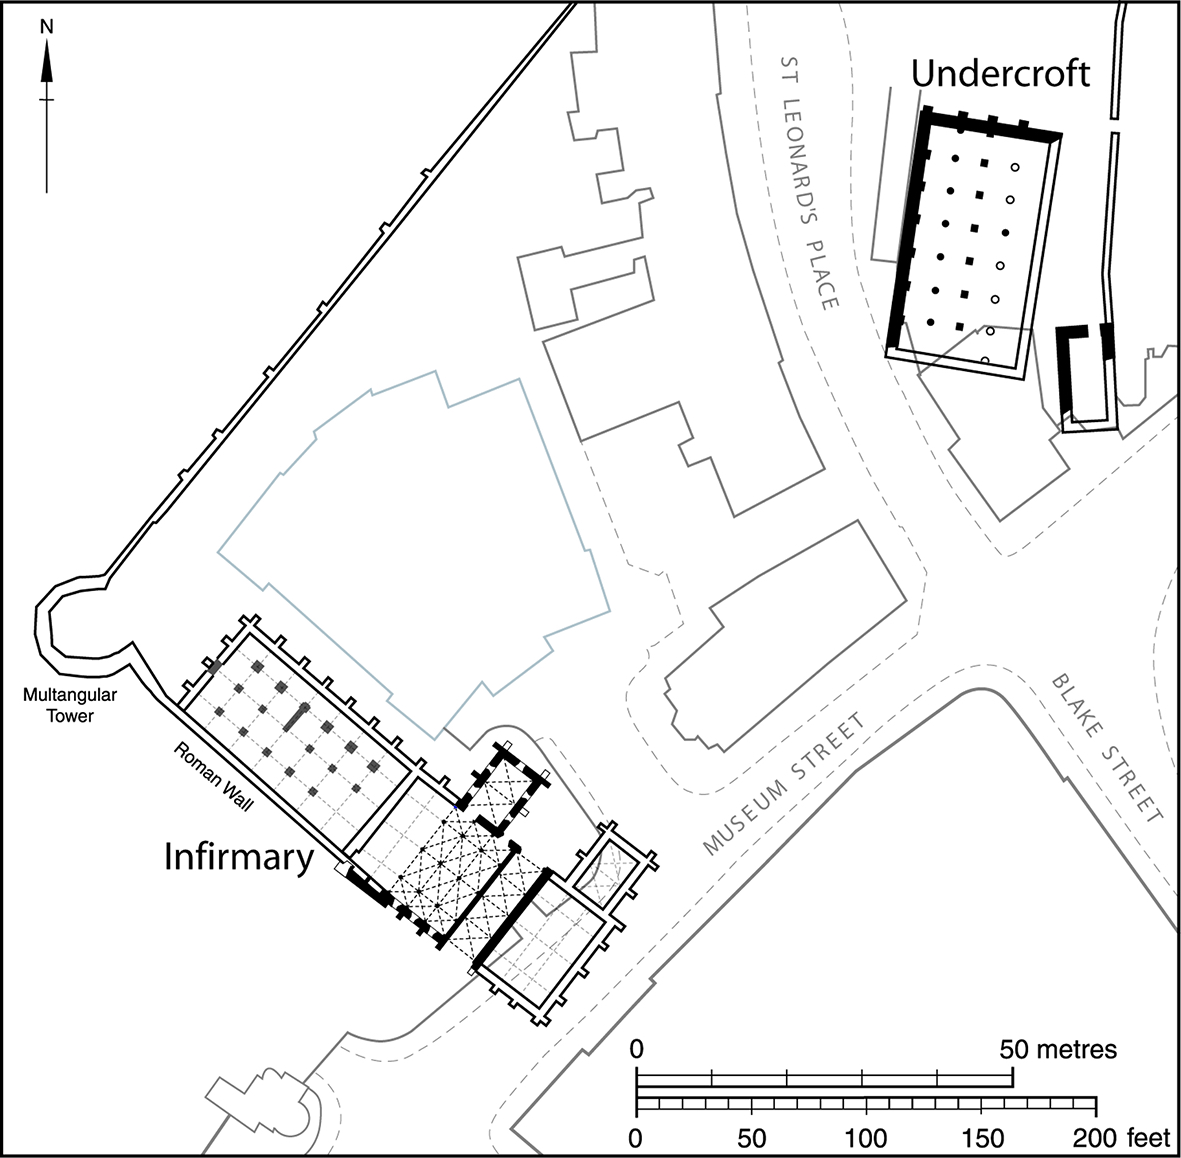
\includegraphics[width=\linewidth]{figures/Pereda-Figure01}
 		\caption{St Leonard’s Hospital plan.
    {\normalfont\scriptsize \\ Obtained from \textcite[100, fig. 37]{Thomas_2002}.
              }}
 		\label{fig:Pereda-Figure01}
 	\end{figure}
 
 The hospital assisted permanent invalids, the chronically ill, and the acutely ill, in addition to the orphans who attended the attached grammar and singing school. Inmates were allowed to stay until they were recovered and capable of working. They were nursed by the sisters, but other than evidence for the purchase of medicines, not much is known about the medical treatments provided at St Leonard’s Hospital \parencites[5,12-15]{Cullum_1991}[21]{Dainton_1961}[97]{Dean_2008}[134]{Goldberg_1992}{Page_1974}[78,109]{Palliser_2014}.
 
 \IJSRAsubsection{History}
Documentary evidence establishes that St Leonard’s Hospital was founded ca.\,936 by King Athelstand, as the Hospital of St Peter, and was located on the western corner of the York Roman fortress. It received the royal privilege of “Petercorn”, though which it was granted corn from all the fields in the diocese. The hospital was re-founded as St Leonard’s Hospital in the \nth{11} century\AD on the orders of King Stephen, and survived until December \nth{1}, 1538, when the hospital was forced to surrender its properties to the Crown 
\parencite[288]{Palliser_2014}. This situation left the city of York lacking a hospital from the time of Henry VIII until the first half of the \nth{18} century\AD \parencite{YorkMuseumGardens_2016}.
\IJSRAsubsection{Hospital complex}
Archaeological excavation suggests that parts of earlier structures were incorporated in the foundations of the medieval hospital. Of the structures that composed St Leonard’s hospital, only a gate, the chapel, and the infirmary (with vaulted under croft) remain in situ. During excavation, part of the stone drain of the hospital was discovered, indicating the existence of a complex drainage system that took the sewage from the infirmary out of the hospital´s precinct \parencite{Johnson_2014}, which would have helped to maintain the hospital in a higher standard of cleanliness than the average domestic living space.
The Rule of 1295 establishes that St Leonard’s was organised around two courtyards. One of them was for the church and the brothers, and the other courtyard was dedicated to the actual hospital. The hospital precinct could be accessed through two doors, one of which was located at the infirmary and the other of which, known as Watergate, was located on Blake Street, where bread, meat and ale were provided weekly to the alms \parencites[8-9,28-29]{Cullum_1991}[17]{Cullum_1999}{Johnson_2014}[151]{Palliser_2014}[116]{Raine_1955}[314]{Rawcliffe_2004}.
Extensive building activity occurred during the \nth{13} century\AD, including the enlargement of the infirmary. At this time, St Leonard’s was known to have had a church, school, orphanage, hospital, Master’s house, residences for the brothers and sisters, a tannery, smithy, brew house, horse mill, carpenter´s shop, and stables 
\parencites[99]{Dean_2008}[116]{Raine_1955}. This indicates that St Leonard’s Hospital was almost completely self-sufficient. These production centres were not only employed to supply the hospital; St Leonard’s also participated in a range of both commercial and charitable activities, exchanging the goods produced at the hospital and providing for the poor.

 \IJSRAsubsection{Inhabitants}
By the late \nth{13} century\AD, the hospital started accepting lepers, causing the number of inmates to peak at over \num{220} individuals, as well as 23 orphans \parencites[6,10]{Cullum_1991}[151]{Palliser_2014}. The hospital could not have maintained this figure overtime, due to a decrease in its financial income. 
Moreover, in the \nth{14} century\AD, due to its precarious economic state, the hospital started accepting the entrance of a large number of corrodians. They were old, wealthy individuals, who paid in cash or in kind to spend the rest of their lives in the hospital, no matter their health conditions. 
However, the expense corrodians incurred is still likely to have been greater than the income they brought to the hospital \parencites[235]{Brodman_2009}[6]{Cullum_1991}. This practice can be interpreted as an early sign of hospitals as providers of remunerated services, rather than just charitable institutions, as well as the medieval precursor of homes for the elderly.
Archaeological evidence
Material remains recovered during excavations at the site include animal bones, glass artefacts, pottery, and a bronze seal ring \parencite{Johnson_2014}. These can be used to obtain information about the daily life of the hospital’s inhabitants. Their diet was known to be more varied and of a better quality than the average members of York’s population, which would have contributed to the inmates’ recovery. 
The everyday menu at the hospital included beef, mutton, pork, beans, honey, bread, ale, and pottage, but lacked fresh fruits and vegetables, which were not widely consumed in medieval society \parencites[16-17]{Cullum_1991}[19]{Cullum_1999}. 
Evidence for the hospital’s wealth can be observed in the infirmary decoration, which included decorated ridge tiles, glazed floor tiles and decorated window glass \parencite[101]{Dean_2008}. 
\IJSRAseparator
 \IJSRAsection{St Bartholomew’s Hospital, London}
The site of the medieval hospital of St Bartholomew in London has not been excavated completely, as it is located beneath the modern St Bartholomew’s Hospital. However, rescue archaeology has been carried out and some material has been recovered.
\IJSRAsubsection{History}
In situations such as this, the work carried out by historians is fundamental to shed light on the activities of the hospital. St Bartholomew’s Hospital (\cref{fig:Pereda-Figure02}) %XXX
was originally founded ca.\,1123 by the adventurer Rahere, with the aid of the Bishop of London, and was re-founded in the time of Henry\,VIII. During this period, the hospital’s income relied on donations collected by a representative sent into towns on behalf of the hospital \parencite[19,42]{Dainton_1961}. 
The importance of this hospital lies in the fact that it is the oldest hospital in England which has continued caring for the sick at its original site since its foundation \parencite[35]{Dainton_1961}. 
Additionally, it was one of the first hospitals in the country to provide education for children \parencite[21]{Rawcliffe_1999}. 

%	\begin{figure}
%		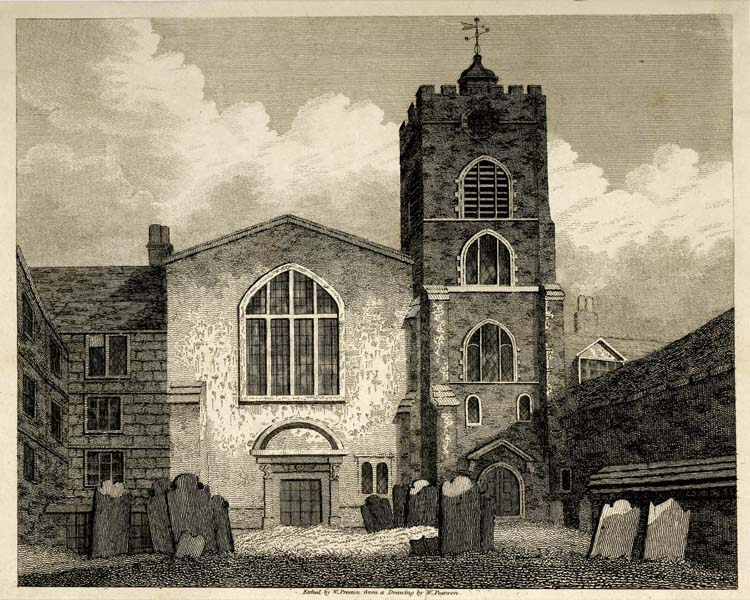
\includegraphics[width=\linewidth]{figures/Pereda-Figure02}
%		\caption{Engraving from 1810 depicting St Bartholomew’s the Great Church, the only surviving element of the original medieval hospital located at the site of the modern St Bartholomew’s Hospital. Artefact ID No.: A19933. Retrieved 20 August 2016.
%		{\normalfont\scriptsize \\ \copyright\ Museum of London}}
%		\label{fig:Pereda-Figure02}
%	\end{figure}

\IJSRAsubsection{Treatments employed at St Bartholomew’s}
In the \nth{14} century\AD, a group of four Augustinian nuns assisted the inmates while living communally within the hospital’s precinct. As was usual in medieval times, the care they provided for the sick was based on spiritual relief and religious well-being, delivered through religious sacraments and participation in religious services. 
Nevertheless, evidence for some kind of medical treatments practiced at the hospital can be found in, for example, Breviarium Bartholomei, written by the priest and medical writer, John Mirfield \parencite[36-37]{Dainton_1961}. 
This occasionally included the employment of charms and other magical features, such the selection of specific days of the month to perform bloodletting \parencite[35-36]{Rider_2012}. 
It was not until after the hospital’s re-foundation, which took place in 1546, that staff with actual medical knowledge were employed. The hospital staff included surgeons, physicians and barbers, in addition to the apothecary who prepared the medicines prescribed by the physicians \parencite[38-39]{Dainton_1961}. This demonstrates a change within hospital treatment, as well as societal attitudes.  
The continuous running of St Bartholomew’s exhibits in a clear way the transformation of former religious medical care into an expert scientific discipline, marked at this site by the advances made on the research of the circulatory system and modern surgery between the \nth{17} and \nth{18} centuries.
\IJSRAseparator
\IJSRAsection{St Mary Spital, London}
The Priory and Hospital of the Blessed Virgin Mary without Bishopsgate (\cref{fig:Pereda-Figure03}), %XXX FIG
known as St Mary Spital, was located in north-east London, and grew to be the largest Medieval hospital in London \parencite[60]{Bowers_2007}. It has been progressively surveyed over the last century, and is therefore one of the best-excavated medieval hospitals. 

%	\begin{figure}
%		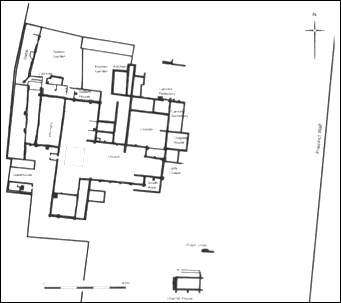
\includegraphics[width=\linewidth]{figures/Pereda-Figure03}
%		\caption{St Mary Spital plan.
%		        {\normalfont\scriptsize \\ Obtained from \textcite[98, fig. 37]{Thomas_2002}.
%		                  }}
%		\label{fig:Pereda-Figure03}
%	\end{figure}


\IJSRAsubsection{History}
St Mary Spital was founded at the beginning of the \nth{12} century\AD by a group of wealthy London merchants, and dissolved under Henry VIII in 1539, leading to the development of the former parish of Spitalfields. Initially, the hospital only assisted the poor and the sick, but through time it also cared for the well-being of pilgrims, migrants, pregnant women, children under the age of seven, and the elderly \parencites[26]{Phillpotts_1997}[48-49]{Thomas_2002}{Unknown_1957}[60-61]{White_2007}.
\IJSRAsubsection{Hospital complex}
The original hospital consisted of a small rectangular structure, most of which was dedicated to housing 13 inmates, and the rest of which was a chapel. This spatial organisation enabled the inmates to see the altar from their beds, which was thought to be indispensable for their recovery \parencites[91]{Phillpotts_1997}[98]{Thomas_2002}.
The second infirmary, dating to the hospital’s re-foundation, was a T-shaped structure divided by a church lying in the centre, forming two separate infirmaries with different entrances, between which the sexes were divided. The hospital included 60 beds, 30 for men and 30 for women, placed against the walls and separated by a central aisle \parencites[37]{Phillpotts_1997}[99]{Thomas_2002}. 
In the \nth{14} century\AD, the old infirmary became a chapel, and a new two-storey structure was built to house the new infirmary. Here, the sexes were likely to have been separated over the two floors. This structure held 90 shared beds and, therefore, possibly up to 180 inmates.
Excavations have revealed the presence of a hearth in the northeast corner of the ground floor, where the sisters might have warmed up food and/or prepared herbal remedies. Soon after its construction, the infirmary was expanded due to the increasing number of individuals entering the hospital \parencites[47]{Phillpotts_1997}[99]{Thomas_2002}[59]{White_2007}. 
After the \nth{14} century\AD, timber structures were built to house the incoming corrodians \parencite[104,152]{Thomas_2002}.
To the north of the infirmary was the refectory, where the brothers ate while listening to passages from the Bible, as was also the case at St Leonard’s Hospital. 
To the north-west was the kitchen \parencites[51]{Phillpotts_1997}[100]{Thomas_2002}; 
towards the west of the infirmary was a cemetery in which the deceased were buried in nine rows, each row with a maximum of 25 burials \parencite[59]{White_2007}; and the brothers’ dormitory was located towards the east, on a first-floor level, with the chapter house and storage area underneath. The southern area of the precinct was used for agricultural purposes and to house animals.

The sisters lived originally in a timber house with mortar floor. Their low status can be inferred from the fact that they were the last members to receive a stone structure in which to live, a conclusion that agrees with the documentary evidence \parencites[36]{Phillpotts_1997}[51]{Rawcliffe_1999}[151]{Thomas_2002}.
St Mary Spital, like St Leonard’s, had its own water supply and drains that ran the waste from the kitchens and the latrines out of the precinct of the hospital \parencite[151]{Thomas_2002}. 
\IJSRAseparator
\IJSRAsection{Archaeological evidence}
Through excavation, a set of keys was found in the \nth{13} century infirmary. They might have been used to open lockers owned by the inmates \parencite[99]{Thomas_2002}. In a pit outside the infirmary, a group of 18~wooden bowls and plates, ceramic vessels, and a pair of leather boots were found well preserved, due to waterlogged conditions. The bowls (\cref{fig:Pereda-Figure04}), %XXX FIG
which have different marks that might have indicated their users, were probably used to feed the sick \parencites[68]{Egan_2007}[99]{Thomas_2002}. 
Nearby, a large number of animal bones were uncovered and used to obtain information about the diet provided at the hospital, which included high proportions of fish and meat \parencite[59,113-114]{Phillpotts_1997}.
In another pit, seven gold coins issued under the kingdom of Henry\,VIII were discovered. These coins were thought to protect against evil through the impressed image of the archangel St Michael and the inscription in Latin: \enquote{Through your cross, save us, Christ, Redeemer.}  \parencite[70]{Egan_2007}. 
These are a clear example of magical charms employed to prevent and treat sickness within Christian contexts. 
At least \num{10500} individuals were buried in the hospital’s cemetery. These skeletal remains provide insight into the kinds of patients for which the hospital cared.  Burials are varied; alongside simple interments lacking coffins and not always aligned in the east-west orientation, there were also high-status individuals buried in lead or stone coffins. Five tombs containing individuals identified as priests included a pewter calyx and a paten for sacramental duties after resurrection. 
An interesting feature is the presence of mass burials in which the deceased are facing downwards, which might evidence a plague that spread in London before the Black Death \parencites[61]{Bowers_2007}[252]{Brodman_2009}[73]{Egan_2007}[101]{Thomas_2002}[61]{White_2007}.
A large number of the individuals interred in the cemetery present skeletal pathologies, elucidating diseases from which the citizens of medieval London may have suffered. For example, several individuals presented lesions consistent with diffuse idiopathic skeletal hyperostosis (DISH); a medical condition caused by a diet rich in animal fats and expressed through the fusion of vertebrae and the overgrowth of bone. This disease has been associated particularly with male members of increasing age within the higher clergy during the Middle Ages, who were a minority able to access plenty of food supplies. 
They may also have suffered from obesity and diabetes mellitus, risk factors to developing DISH
\parencites[361-362]{Rogers_2001}{Verlaan_2007}[1763]{Waldron_1985}[62]{White_2007}.
Evidence of surgical treatments performed at the hospital can also be identified in the skeletal remains. 
Skeletal trauma shows signs of healing, suggesting that individuals were surviving procedures such as trepanations and lower limb amputations \parencite[63-64]{White_2007}. This change within medical practice, already appreciated at the other sites, might have been a response to the society’s changing needs.
Sheets of metal plates were found at three burials containing textile remains in the inner side, similar to the finds recovered at Merton Priory, London, and Gilbertine Priory of St Andrew, York. These metal plates might have been used to protect long-term bandages, which could have contained medical preparations \parencite[70-71]{Bowers_2007}. 
Besides this evidence of sophisticated medical practice, other interesting artefacts proving a religious perspective on health and death were also found at some burials of the Mary Spital cemetery. They include five papal lead seals, bullae, dating back to the \nth{14} century\AD. They have the name of Pope Urban\,VI inscribed upon them, and used to be attached to documents that proved that the deceased have had their sins pardoned \parencites[69]{Phillpotts_1997}[70,72]{White_2007}.

%	\begin{figure}
%		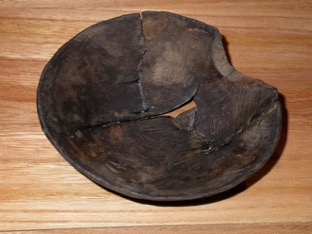
\includegraphics[width=\linewidth]{figures/Pereda-Figure04}
%		\caption{One of the wooden bowls recovered from St Mary Spital. They contained scratched marks and might have been used to feed the sick.
%		{\normalfont\scriptsize \\ \copyright\ Museum of London; Image obtained from Museum of London. Artefact ID No.: NRF88[1286]<611>. Retrieved 20 August 2016.}}
%	\label{fig:Pereda-Figure04}
%   \end{figure}


\IJSRAseparator
\IJSRAsection{Discussion and Conclusion}
Only through the combination of all sources of evidence (historical documents and material remains) available, can a complete and comprehensible picture of past societies be obtained. When material evidence cannot be accessed, such as in the case of St Bartholomew’s Hospital, or has been lost, documents can fill the gaps. Conversely, archaeological remains can support or challenge what is written in the documentary evidence. Investigations of medieval hospitals need to be approached from historical and archaeological perspectives in order to allow researchers to provide the most accurate conclusions possible. 
As indicated by the documentary and material evidence exhibited for the three case studies investigated in the present paper, the complex of medieval hospitals was similar to the monastic design. They usually consisted of a chapel, cloisters, refectory, infirmary, and gardens where agricultural activities for commercial and self-provisioning purposes, and human burials took place. 
The evolution of hospital complexes is not easily understood, due to their constant development and refurbishment, which in cases such as St Mary Spital was due to the continuous need for larger structures to house the increasing numbers of incoming inmates \parencites[69,117-118]{Henderson_2006}[27]{Malcom_2014}[41,43]{Orme_1995}[35]{Rawcliffe_1999}.
Medieval hospitals based their income on the donations made by wealthy individuals who wanted their charitable acts to be considered in purgatory. However, due to a decrease in income, from the \nth{14} century\AD onwards, hospitals began to accept more corrodians than cremetts \parencites[69]{Dean_2008}[207]{Malcom_2014}. 
Hospitals originally operated as religious institutions, worship being their primary function. This is evidenced by the central position that chapels occupied within the infirmaries at St Mary Spital, St Bartholomew’s and St Leonard’s, and the obligation for the sick to attend their services. Brothers lived in the hospitals accompanied by sisters who assisted the inmates (old, wealthy individuals, the poor, the sick, orphans, and pregnant women), and the lay workers who behaved to some extent as religious individuals, attending services and living in a community in which men were separated from women, as has been exhibited in the cases of St Leonard’s and St Mary Spital. 
Archaeological excavations provide more material evidence related to the spiritual well-being of the inmates than to medical treatments; evidence for the latter is rare, and consists mainly of evidence for interventions on skeletal remains, such as those at St Mary Spital, as no medical instrument has been clearly identified \parencite[65,76]{Bowers_2007}. 
It is necessary to take into account that medieval medical implements are likely to have greatly differed from modern ones and might not be easily recognisable as such. Additionally, there might be some level of predisposition from researchers to interpret finds recovered at medieval hospitals as religious rather than scientific, due to the ecclesiastical nature of the sites. 
Religious relief, the reconciliation of a soul cleansed of sins with God, was the way to cure or alleviate physical pains, which were understood as punishments from God \parencites[12-13,96]{Biller_2001}[42-43]{Rawcliffe_1995}. 
Besides treating the inmates’ spiritual health, the treatments carried out by nuns consisted of cleaning, feeding, clothing and housing the patients; acts likely to have contributed to the inmates’ physical recovery, even if divine intervention alone was credited. Material evidence from St Mary Spital and St Leonard’s indicates that the diet consumed by the people living at medieval hospitals was varied, and better than regular citizens’ food. Some of this food was produced on the grounds of the hospital, while other products were obtained through donations \parencites[76]{Egan_2007}[208]{Malcom_2014}.
Nevertheless, the epidemic diseases that spread during the \nth{14} century\AD provoked a stronger engagement of individuals with medical knowledge indicated by the survival of medical manuscripts, 
such as Breviarium Bartholomei from St Bartholomew’s Hospital \parencite[6,16-22]{Stell_1996}. 
In conclusion, early medieval hospitals provided a broader range of services than their modern counterparts and might be better regarded as charitable institutions, rather than strict medical centres in their modern significance. Nevertheless, from the \nth{14} century\AD onwards, advances in medicine were developed, and were slowly incorporated into these religious hospitals, until scientific treatments eventually replaced the exclusively religious care that was originally central to medieval hospitals. 

\iffalse
Illustrations
Figure 1. St Leonard’s Hospital plan. Obtained from Dean, 2008: 100, figure 37.
Figure 2. Engraving from 1810 depicting St Bartholomew’s the Great Church, the only surviving element of the original medieval hospital located at the site of the modern St Bartholomew’s Hospital. Artefact ID No.: A19933. ©Museum of London. Retrieved 20 August 2016.
Figure 3. St Mary Spital plan. Obtained from Thomas, 2002: 98, figure 37.
Figure 4. One of the wooden bowls recovered from St Mary Spital. They contained scratched marks and might have been used to feed the sick. Image obtained from Museum of London. Artefact ID No.: NRF88[1286]<611>. ©Museum of London. Retrieved 20 August 2016.
\fi
\IJSRAclosing%<---- don’t change this!
\end{document}
\documentclass{ijsra}
%----- will be part of version 0.5
\renewcommand\AD{{\,AD\xspace}}
\renewcommand\BC{{\,BC\xspace}}
%--------
\def\IJSRAidentifier{\currfilebase}%<<<< DO NOT change this line
\def\shorttitle{Elephant motifs on Greek coinage}
\def\maintitle{Elephant motifs on Graeco-Bactrian  and Indo-Greek~coinage}
\def\cmail{rahul.raza@some.ox.ac.uk}
\def\keywords{Hellenistic, Graeco-Bactrian, Indo-Greek, Numismatics, Royal Ideology, Elephants}
%\def\keywordname{}
\def\abstract{The \IJSRAsection{Abstract} Graeco-Bactrian and Indo-Greek kings of Hellenistic Bactria and India are known mainly through their coins. This article studies elephant motifs on the coins. The study involves content and context analysis of the iconography to gain an understanding of the meaning and function of the elephant imagery. This paper will argue that Graeco-Bactrian and Indo-Greek kings used elephant symbolism to express royal power in a cross-cultural context. Hellenocentric approaches that overlook the local context to royal power in Hellenistic kingdoms are challenged. This helps provide a clearer understanding of how Hellenistic kings established and maintained control over kingdoms with multi-ethnic populations.}
\def\authorone{Rahul Raza}
\undef\bioone%{\emph{Master's student?}}% needs to be added
\def\affilone{Classical Archaeology, University of Oxford}
\def\coinindia{Educational and non-commercial use allowed by © \cite{Coin}.}
\iffalse
Appian, White, H., 2014: Roman History. Cambridge: Harvard University Press.
Aristotle, Peck, A.L., 2014: History of Animals. Cambridge: Harvard University Press.
Arrian, Hammond, M., Atkison, J., 2013: Alexander the Great: The Anabasis and the Indica. Oxford: Oxford University Press.
Justin, Yardley, J.C., Develin, R., 1994: Epitome of the Philippic history of Pompeius Trogus. Atlanta: Scholars Press.
Plutarch, Babbitt, F.C., 1957: Moralia, in fifteen volumes, with an English translation by Frank Cole Babbitt. Cambridge: Harvard University Press 
Polybius; Waterfield, R., McGing, B., 2010: The Histories. Oxford: Oxford University Press. 
Strabo, Jones, H.L., Sterrett, J.R.S., 2014:  Geography. Cambridge: Harvard University Press.

\fi
\begin{filecontents}{\IJSRAidentifier.bib}
@incollection{Abdullaev1995,
    author = {Abdullaev, K.},
    title = {Armour of ancient Bactria},
    pages = {163--180},
    editor = {Invernizzi, A.},
    booktitle = {In the land of the gryphons: papers on Central Asian archaeology in antiquity},
    publisher = {Le lettere},
    location = {Firenze},
    year = {1995},
    }

@incollection{Alonso2013,
    author = {Alonso Troncoso, V.},
    title = {The Diadochi and the zoology of kingship: The elephants},
    pages = {254--270},
    editor = {Alonso Troconso, V. and Anson, E.},
    booktitle = {After Alexander: The Time of the Diadochi (323-281 BC)},
    publisher = {Oxbow Books},
    location = {Oxford},
    year = {2013},
    }

@article{Alonso2014,
author = {Alonso Troncoso, V.},
year  = {2014},
title  = {The Zoology of Kingship: From Alexander the Great to the Epigoni (336 – c. 250 BC)},
journaltitle = {ANABASIS},
volume = {5}, 
pages = {53–75},
}

@book{Alter2004,
	author = {Alter, S.},
	title = {Elephas Maximus},
	publisher = {Harcourt},
	location = {Orlando},
	year = {2004},
	}


@article{Bannikov2013,
   author = {Bannikov, A.V. and Popov, A.},
   title = {War elephants in Greco-Bactrian and Indo-Greek Armies},
   pages = {1206--1211},
   journaltitle = {World Applied Sciences Journal},
   volume = {27},
   year ={2013},    
    }

@book{Billows1995,
    author = {Billows, R.},
    title = {Kings and colonists: Aspects of Macedonian imperialism},
    publisher = {Brill},
    location = {Leiden},
    year = {1995},
    }

@article{Bopearachchi1990,
author = {Bopearachchi, O.}, 
year = {1990},
title = {Graeco-Bactrian Issues of Later Indo-Greek Kings},
journaltitle = {The Numismatic Chronicle},
volume  = {150}, 
pages = {79–103}
}

@book{Bopearachchi1991,
    author = {Bopearachchi, O.},
    title = {Monnaies gréco-bactriennes et indo-grecques: Catalogue raisonné},
    publisher = {Bibliothèque nationale},
    location = {Paris},
    year = {1991},
    }

@book{Bopearachchi1993,
    author = {Bopearachchi, O.},
    title = {Indo-Greek, Indo-Scythian and Indo-Parthian coins in the Smithsonian Institution},
    publisher = {National Numismatic Collection, Smithsonian Institution},
    location = {Washington},
    year = {1993},
    }

@incollection{Bopearachchi2007,
    author = {Bopearachchi, O.},
    title = {Some Observations on the Chronology of the Early Kushans},
    pages = {41--54},
    editor = {Gyselen, R.},
    booktitle = {Des Indo-Grecs aux Sassanides: Données pour l’histoire et la géographie historique},
    publisher = {Groupe pour l’étude de la civilisation du Moyen-Orient},
    location = {Bures-sur-Yvette},
    year = {2007},
    }

@incollection{Bopearachchi2011,
    author = {Bopearachchi, O.},
    title = {The emergence of the Graeco-Baktrian and Indo-Greek kingdoms},
    pages = {47--50},
    editor = {Wright, N.L.},
    booktitle = {Coins from Asia Minor and the East, Selections from the Colin E. Pitchfork Collection},
    publisher = {Numismatic Association of Australia},
    location = {Adelaide},
    year = {2011},
    }

@incollection{Bopearachchi2015,
author = {Bopearachchi, O.},
year = {2015},
title = {The Evidence of the Overstrikes for the Reconstruction of the History of the Indo-Greeks},
editor = {Bopearachchi, O.},
booktitle = {From Bactria to Taprobane: Selected Works of Osmund Bopearachchi, Central Asian and Indian Numismatics}, 
volume = {1},
pages = {1171–1200},
location = {New Delhi},
publisher = {Manohar Publishers \& Distributors},}

@article{Bukharin2004,
   author = {Bukharin, M.},
   title = {Early royal dynasties in the Puranas, epics and classical tradition},
   pages = {51--80},
   journaltitle = {Indologica Taurinensia},
   volume = {30},
   year ={2004},    
    }

@book{Campbell2015,
author = {Campbell, J. and Zimmer, H.},
year = {2015},
title = {Myths and Symbols in Indian Art and Civilization},
publisher = {Princeton University Press},
location = {Princeton},
}

@online{Coin,
   title = {Coin India: The Virtual Museum of Indian Coins},
   url = {http://coinindia.com/},
   shorthand = {Coin India},
   urldate = {2016-08-30},
    }

@incollection{Cribb2011,
    author = {Cribb, J.},
    title = {Money as a marker of cultural continuity and change in Central Asia},
    pages = {333--375},
    editor = {Cribb, J. and Herrmann, G.},
    booktitle = {After Alexander: Central Asia before Islam},
    publisher = {Oxford University Press},
    location = {Oxford},
    year = {2011},
    }

@book{Curtis2007,
    editor = {Curtis, V. and Errington, E.},
    title = {From Persepolis to the Punjab: Exploring ancient Iran, Afghanistan and Pakistan},
    publisher = {British Museum Press},
    location = {London},
    year = {2007},
    }

@book{Dahmen2007,
author = {Dahmen, K.},
year = {2007},
title = {The legend of Alexander the Great on Greek and Roman Coins},
publisher = {Routledge},
location = {New York}}

@book{Dhammika2005,
    author = {Dhammika, S.},
    title = {The Buddha and his disciples},
    publisher = {Buddhist Publication Society},
    location = {Kandy},
    year = {2005},
    }

@article{Dhavalikar1981,
   author = {Dhavalikar, M.},
   title = {Antiquity of Ganesa: The numismatic evidence},
   pages = {137--145},
   journaltitle = {Indologica Taurinensia},
   volume = {8--9},
   year ={1981},    
    }

@incollection{Erickson2013,
author = {Erickson, K.}, 
year = {2013},
title = {Seleucus I, Zeus and Alexander},
editor = {Melville, C. and Mitchell, L.},
booktitle = {Every Inch a King: Comparative Studies on Kings and Kingship in the Ancient and Medieval Worlds},
pages = {109–128},
location = {Boston},
publisher = {Brill}}

@article{Fussman1993,
author = {Fussman, G.},
year = {1993},
title = {Ménandre l'Indo-grec ou Paul Demiéville revisité},
journaltitle = {Journal Asiatique},
volume = {281},
issue = {1-2},
pages = {61–137}}

@book{Gonda1966,
    author = {Gonda, J.},
    title = {Ancient Indian kingship from the religious point of view},
    publisher = {Brill},
    location = {Leiden},
    year = {1966},
    }

@book{Green1993,
    author = {Green, P.},
    title = {Alexander to Actium: The historical evolution of the Hellenistic age},
    publisher = {University of California Press},
    location = {Berkeley},
    year = {1993},
    }

@book{Gupta1983,
    author = {Gupta, S.K.},
    title = {Elephant in Indian art and mythology},
    publisher = {Abhinav Publications},
    location = {New Delhi},
    year = {1983},
    }

@incollection{Hollis2011,
    author = {Hollis, A.},
    title = {Greek Letters in Hellenistic Bactria},
    pages = {104--118},
    editor = {Obbink, D. and Rutherford, R. B.},
    booktitle = {Culture in pieces: Essays on ancient texts in honour of Peter Parsons},
    publisher = {Oxford University Press},
    location = {Oxford},
    year = {2011},
    }

@article{Holt1981,
author = {Holt, F. L.},
year = {1981},
booktitle = {The Euthydemid Coinage of Bactria: Further Hoard Evidence from Ai Khanoum},
journaltitle = {Revue Numismatique},
volume = {23},
pages = {7–44}}

@book{Holt1999,
    author = {Holt, F. L.},
    title = {Thundering Zeus: The making of Hellenistic Bactria},
    publisher = {University of California Press},
    location = {Berkeley},
    year = {1999},
    }

@book{Holt2003,
    author = {Holt, F. L.},
    title = {Alexander the Great and the mystery of the elephant medallions},
    publisher = {University of California Press},
    location = {Berkeley},
    year = {2003},
    }

@book{Holt2005,
    author = {Holt, F. L.},
    title = {Into the land of bones: Alexander the Great in Afghanistan},
    publisher = {University of California Press},
    location = {Berkeley},
    year = {2005},
    }

@book{Holt2012,
    author = {Holt, F. L.},
    title = {Lost World of the Golden King: In Search of Ancient Afghanistan},
    publisher = {University of California Press},
    location = {Berkeley},
    year = {2012},
    }

@book{Howgego1995,
    author = {Howgego, C.},
    title = {Ancient history from coins},
    publisher = {Routledge},
    location = {London},
    year = {1995},
    }

@book{Hudson2008,
author = {Hudson, D. D.},
year = {2008},
title = {The Body of God: An Emperor's Palace for Krishna in Eighth-Century Kanchipuram},
location = {Oxford},
publisher = {Oxford University Press}}

@book{Huntingford1980,
author = {Huntingford, G. W. B.},
year = {1980},
title = {The Periplus of the Erythraean Sea, by an Unknown Author},
location = {London},
publisher = {Hakluyt Society}}

@article{Iossif2010,
   author = {Iossif, P. P. and Lorber, C.},
   title = {The Elephantarches Bronze of Seleucos I Nikator},
   pages = {147--164},
   journaltitle = {Syria},
   volume = {87},
   year ={2010},    
    }



@article{Kalita1997,
   author = {Kalita, S.},
   title = {Portraits of rulers on Greco-Bactrian and Indo-Greek coins},
   pages = {7--24},
   journaltitle = {Notae Numismaticae - Zapiski Numizmatyczne},
   volume = {2},
   year = {1997},    
    }

@incollection{Lerner2009,
    author = {Lerner, Judith A.},
    title = {Animal headdresses on the sealings of the Bactrian documents},
    pages = {215--226},
    editor = {Sundermann, W. and Hintze, A. and de Blois, F.},
    booktitle = {Exegisti Monumenta: Festschrift in Honour of Nicholas Sims-Williams},
    publisher = {Harrassowitz Verlag},
    location = {Wiesbaden},
    year = {2009},
    }

@book{Lerner1999,
    author = {Lerner, Jeffrey D.},
    title = {The Impact of Seleucid Decline on the eastern Iranian plateau},
    subtitle = {The foundations of Arsacid Parthia and Graeco-Bactria},
    publisher = {Steiner},
    location = {Stuttgart},
    year = {1999},
    }

@article{Libanius,
editor = {Downey, G.}, 
year = {1959},
title = {Libanius' Oration in Praise of Antioch (Oration XI)},
journaltitle = {Proceedings of the American Philosophical Society},
volume = {103},
issue = {5}, 
pages = {652–686}}

@incollection{MacDowall2007b,
    author = {MacDowall, D. W.},
    title = {Coinage from Iran to Gandhara},
    pages = {233--266},
    editor = {Srinivasan, D.},
    booktitle = {On the cusp of an era: art in the pre-Kusana world},
    publisher = {Brill},
    location = {Leiden},
    year = {2007},
    }

@incollection{MacDowall2007a,
    author = {MacDowall, D. W.},
    title = {The Eras of Demetrius, Eucratides and Azes},
    pages = {103--110},
    editor = {Gyselen, R.},
    booktitle = {Des Indo-Grecs aux Sassanides: données pour l’histoire et la géographie historique},
    publisher = {Groupe pour l’étude de la civilisation du Moyen-Orient},
    location = {Bures-sur-Yvette},
    year = {2007},
    }

@incollection{MacDowall2007c,
author={MacDowall, D. W.},
year = {2007},
title = {Numismatic Evidence for a Chronological Framework for Pre-Kaniskan Art, from Kalchayan to Gandhāra},
editor = {D. Srinivasan}, 
booktitle = {On the cusp of an era: art in the pre-Kusana world},
pages = {233–266},
location = {Leiden},
publisher = {Brill}}

@book{Mairs2014,
    author = {Mairs, R.},
    title = {The Hellenistic Far East: Archaeology, Language, and Identity in Greek Central Asia},
    publisher = {University of California Press},
    location = {Berkeley},
    year = {2014},
    }

@incollection{Mairs2015,
    author = {Mairs, R.},
    title = {Bactria and India},
    pages = {637--650},
    editor = {Eidinow, E. and Kindt, J.},
    booktitle = {The Oxford handbook of ancient Greek religion},
    publisher = {Oxford University Press},
    location = {Oxford},
    year = {2015},
    }

@phdthesis{Marcinkiewicz-Joseph2016,
author = {Marcinkiewicz-Joseph, F. A.}, 
year = {2016},
title = {Demetrius I of Bactria: An analysis of Hellenistic royal power through numismatic evidence},
institution = {Department of History, University of Houston, Houston},
pubstatus = {unpublished},}

@incollection{Maritz2004,
    author = {Maritz, J.},
    title = {The Face of Alexandria – the Face of Africa?},
    pages = {41--66},
    editor = {Hirst, A. and Silk, M. S.},
    booktitle = {Alexandria, real and imagined},
    publisher = {Ashgate},
    location = {Aldershort, Hampshire},
    year = {2004},
    }

@incollection{Narain1991,
    author = {Narain, A. K.},
    title = {Gaṇeśa},
    subtitle = {A Protohistory of the Idea and the Icon},
    pages = {19--48},
    editor = {Brown, R. L.},
    booktitle = {Ganesh: studies of an Asian god},
    publisher = {State University of New York Press},
    location = {Albany},
    year = {1991},
    }

@book{Narain2003,
    author = {Narain, A. K.},
    title = {The Indo-Greeks},
    subtitle = {Revisited and supplemented},
    publisher = {B.R. Publishing},
    location = {New Delhi},
    year = {2003},
    }

@book{Pfrommer1993,
    author = {Pfrommer, M.},
    title = {Metalwork from the Hellenized East},
    subtitle = {A catalogue of the collections},
    publisher = {J. Paul Getty Museum},
    location = {Malibu},
    year = {1993},
    }

@incollection{Potter2003,
author = {Potter, D.},
year = {2003},
title = {Hellenistic Religion},
editor = {A. Erskine},
booktitle = {A Companion to the Hellenistic Word}, 
pages = {407–430},
location = {Oxford},
publisher = {Blackwell Publishing}}

@book{Rothkrug2006,
author = {Rothkrug, L.},
year = {2006},
title = {Death, Trust, and Society: Mapping Religion and Culture},
location = {Berkeley},
publisher = {North Atlantic Books}}

@book{Sidky2000,
author = {Sidky, H.},
year = {2000},
title= {The Greek Kingdom of Bactria: From Alexander to Eucratides the Great},
location = {Lanham},
publisher = {University Press of America}}

@article{Smith1986,
   author = {Smith, R. R. R.},
   title = {Three Hellenistic Rulers at the Getty},
   pages = {59--78},
   journaltitle = {The J. Paul Getty Museum Journal},
   volume = {14},
   year ={1986},    
    }

@book{Stanco2012,
    author = {Stančo, L.},
    title = {Greek Gods in the East: Hellenistic iconographic schemes in Central Asia},
    publisher = {Karolinum Press},
    location = {Prague},
    year = {2012},
    }

@book{Stewart1993,
    author = {Stewart, A. F.},
    title = {Faces of Power: Alexander’s image and Hellenistic politics},
    publisher = {University of California Press},
    location = {Berkeley},
    year = {1993},
    }


@book{Strootman2014,
    author = {Strootman, R.},
    title = {Courts and elites in the Hellenistic empires: The Near East after the Achaemenids, c. 330 to 30 BCE},
    publisher = {Edinburgh University Press},
    location = {Edinburgh},
    year = {2014},
    }

@book{Tarn1951,
    author = {Tarn, W. W.},
    title = {The Greeks in Bactria and India},
    publisher = {Cambridge University Press},
    location = {Cambridge},
    year = {1951},
    }

@book{Thonemann2015,
    author = {Thonemann, P.},
    title = {The Hellenistic world: using coins as sources},
    publisher = {Cambridge University Press},
    location = {Cambridge},
    year = {2015},
    }

@book{Trautmann2015,
    author = {Trautmann, T.},
    title = {Elephants and Kings: An Environmental History},
    publisher = {The University of Chicago Press},
    location = {Chicago},
    year = {2015},
    }

@incollection{Treister1999,
    author = {Treister, M.},
    title = {Some classical subjects on the Late Hellenistic Sarmatian Phalerae (to the origin of Phalerae)},
    pages = {565--604},
    editor = {Tsetskhladze, G. R.},
    booktitle = {Ancient Greeks West and East},
    publisher = {Brill},
    location = {Leiden},
    year = {1999},
    }

@book{Whitehead1970,
    author = {Whitehead, R.B.},
    title = {Indo-Greek numismatics},
    publisher = {Argonaut},
    location = {Chicago},
    year = {1970},
    }

@article{Widemann2000,
   author = {Widemann, F.},
   title = {Scarcity of precious metals and relative chronology of Indo-Greek and related coinages (1st Century B.C.-1st Century A.D.)},
   pages = {227--258},
   journaltitle = {East and West},
   volume = {50},
   year ={2000},    
    }

@article{Widemann2003,
   author = {Widemann, F.},
   title = {Maues King of Taxila: an Indo-Greek kingdom with a Saka king},
   pages = {95--125},
   journaltitle = {East and West},
   volume = {53},
   year ={2003},    
    }

@article{Widemann2007,
   author = {Widemann, F.},
   title = {Civil wars and alliances in Bactria and North-Western India after the usurpation of King Eucratides},
   pages = {9--28},
   journaltitle = {East and West},
   volume = {57},
   year = {2007},    
    }

@book{Widemann2009,
    author = {Widemann, F.},
    title = {Les successeurs d’Alexandre en Asie centrale et leur héritage culturel: Essai},
    publisher = {Riveneuve éd},
    location = {Paris},
    year = {2009},
    }

@book{Zimmer2015,
    editor = {Zimmer, H. and Campbell, J.},
    title = {Myths and Symbols in Indian Art and Civilization},
    publisher = {Princeton University Press},
    location = {Princeton},
    year = {2015},
    }
\end{filecontents}

\begin{document}
\IJSRAopening%<<<< DO NOT change this line

\lettrine{T}{he} Persian satrapy of Bactria, centred in present-day Afghanistan, Uzbekistan, and Tajikistan,
was conquered by Alexander the Great in 327\BC.
Afterwards, Bactria was incorporated into the Seleucid Empire, established by Alexander’s general and successor in Asia,
Seleucus Nicator.
In the mid-third century\BC, Bactria became an independent Hellenistic kingdom under the Graeco-Bactrian kings, 
who expanded their territory to include ancient north-west India (now mainly Afghanistan, Pakistan,
and parts of India).
After a period of conflict towards the middle of the second century\BC, the Graeco-Bactrian kingdom became politically divided,
and its Indian territories came under the rule of independent Indo-Greek kings.
While the Graeco-Bactrian kingdom fell to the invasions of nomadic tribes from Central Asia c. 130\BC,
the Indo-Greeks continued to rule until the turn of the first century\AD, when the last king was also deposed by the nomads
\parencites[47--50]{Bopearachchi2011}[3]{Mairs2014}. 

Since literary sources are lacking, Graeco-Bactrian and Indo-Greek history has been reconstructed mainly from coins \parencite[96--97]{Thonemann2015}.
This is possible because the symbols on the coins, such as images and inscriptions, publicised the identity, agenda, and achievements of the ruler who issued them.
While ancient coinage had mainly an economic function, it was widely used for political purposes. This was a result of its wide circulation in everyday life as currency, allowing kings to communicate with their subjects at large \parencite[11,61]{Howgego1995}.
As Aristotle writes, “everybody inspects his coins” \parentext{Arist. HA. 491a; \cite[120]{Holt1999}}.
The iconography of coins was therefore a politically significant choice, and in the words of one scholar, the “most deliberate of all symbols of public identity” \parencite[66]{Thonemann2015}.

This paper studies the representation of royal power through elephants, the most common animal on the coins, and widely represented in ancient visual culture as a symbol of power and divinity \parencites[383--384]{Bopearachchi1991}[11--19]{Gupta1983}[156]{Iossif2010}.
The focus is on three distinct coin types, including the ‘elephant headdress’, the ‘elephant aegis’, and the ‘elephant goad’. Through this analysis, this paper argues that elephant symbolism was legitimised royal authority in a cross-cultural context.  While various studies have been conducted on elephant imagery in Hellenistic royal self-presentation, the conclusion is that ethnic prejudice prevented the animals from becoming more than a symbol of Greek imperial power and conquest \parencites[263--264]{Alonso2013}[69]{Alonso2014}.
This paper challenges these ‘Hellenocentric’ narratives that overlook Graeco-Bactrian and Indo-Greek engagement with local ruling traditions and kingship practices.

\begin{figure}[!htb] %Figure 1
	%\begin{wrapfigure}{O}{0.5\textwidth} 
	\centering
	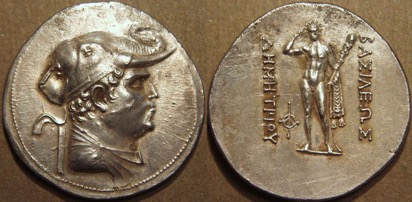
\includegraphics[width=.6\linewidth]{Raza-Figure01}
	\caption{Demetrius I. King wearing elephant headdress / Heracles holding diadem, club, and lion skin.
		{\normalfont\scriptsize \\ \coinindia}}
	\label{fig:Raza-Figure01}
\end{figure}
%\end{wrapfigure}

The first coin type under consideration is the elephant headdress.
This refers to obverse side designs representing the ruler in a headdress resembling an elephant's head.
Although three kings issued the coin type, discussion has centred on the coins of Demetrius I
(c. 200-185\BC) (see \cref{fig:Raza-Figure01}), the Graeco-Bactrian king who first invaded India \parencites[47--48]{Bopearachchi2011}[17--18]{Kalita1997}.
Explanations for the symbolic meaning of the elephant headdress draw mainly on Greek precedent. Originally, the elephant headdress had adorned posthumous Hellenistic representations of Alexander the Great, not unlike the lion skin of Heracles. It is thought that Alexander was being represented as an elephant slayer and that the headdress symbolically alluded to his conquests in India, the land of elephants to the Greeks \parencites[50]{Curtis2007}[335]{Green1993}[104--105]{MacDowall2007a}.
Consequently, the weight of analogy leads to the conclusion that Demetrius’ elephant headdress also commemorated his Indian conquests. If so, Demetrius’ coin type would support negative assessments of Greek engagement with local traditions. The elephant was a sacred animal for ancient Indians and the ascribed symbolism is analogous to the story of the Persian king Cambyses’ killing of the Apis Bull in Egypt \parencite[11--19]{Gupta1983}. Accordingly, it has been said that the symbolism was one of “massacre d’elephant,” representing conquest \parencite[492]{Widemann2009}.

However, the conquest interpretation is at odds with the chronology. Although dates for the Indian campaigns are unavailable, numismatists point out that Demetrius’ elephant headdress coins appear from the outset of his reign, before the new king would presumably have the chance to invade India \parencite[157]{Holt2012}.
Nevertheless, the presupposition that Demetrius was emulating Alexander has led to arguments to the contrary, all of which associate the elephant with India.
Principally, there is the suggestion that the elephant headdress coins indicate that Demetrius’ conquests took place before he became king, presumably as a general of his father Euthydemus I (c. 230-200\BC) \parencite[157]{Holt2012}.
Another is that if not alluding to conquests already made, the elephant headdress represented Demetrius as a ‘second Alexander’, and thus heralding an intention to conquer India in the future \parencites[190]{Sidky2000}[132]{Tarn1951}.
This paper argues against such proposals, instead suggesting that Demetrius’ elephant headdress represented a symbol of royal power accommodating various cultural groups.

First, the authority for Demetrius’ Indian campaigns is Strabo, who describes the conqueror as \enquote*{Δημήτριος ὁ Εὐθυδήμου υἱὸς τοῦ Βακτρίων βασιλέως},
‘Demetrius, son of Euthydemus, the king of the Bactrians’ (Strab. Geo. 11.11.1).
Some read the Greek to mean that Strabo was withholding the royal title from Demetrius, and that Euthydemus was king at this time \parencites[157]{Holt2012}[99]{MacDowall2007c}.
If so, Demetrius’ introduction of the elephant headdress coins might have alluded to his previous Indian conquests under Euthydemus.
However, Strabo’s syntax is structured around Demetrius, and the sentence should read that the latter was both Euthydemus’ son and king of Bactria. The traditional reading is indeed that Demetrius was the king mentioned in the text \parencite[144]{Tarn1951}.
Consequently, Strabo does not support the placing of Demetrius’ Indian campaigns under Euthydemus.

Second, it has been argued that a Greek inscription from Kuliab, Tajikistan, hailing Demetrius as \emph{Kallinikos}, ‘the Glorious Victor’, alludes to his Indian conquests under Euthydemus, the reigning king whom the inscription honours as \emph{Basileus Megiston}, ‘the Greatest of all Kings” \parencites[110]{Hollis2011}[125]{Holt2012}[104--105]{MacDowall2007a}[99]{MacDowall2007c}.
However, the inscription could have been alluding to victories claimed against Antiochus III, the Seleucid king who had unsuccessfully invaded Bactria during the reign of Euthydemus in 208-206\BC \parencite[48]{Bopearachchi2007}.
Polybius’ account of the war indicates that Demetrius was a young man, and thus old enough to have participated in some leading role (Pol. Hist. 11.34).
In addition, the wording of Euthydemus’ epithet suggests that the inscription is describing his successful resistance to Antiochus, who had adopted the title of \emph{Basileus Megas}, ‘the Great King’ \parencites[111]{Hollis2011}[125]{Holt2012}.
Thus, the Kuliab inscription does not necessarily suggest that Demetrius campaigned in India under Euthydemus.

Finally, while the dates cannot be fixed with any certainty, Graeco-Bactrian expansion into India seems improbable during the reign of Euthydemus.
Antiochus invaded India after the Bactrian war, evidently still ruled by independent kings such as Sophagasenus.
Meanwhile, nomads had begun troubling the Graeco-Bactrians, and Polybius writes that Euthydemus warned Antiochus of the mutual threat from an imminent invasion (Pol. Hist.11.34).
Significantly, the loss of Sogdiana – now mainly Tajikistan – coincided with the war with Antiochus, who seemed convinced to make peace with Euthydemus \parencites[38--39]{Holt1981}[135]{Holt1999}.
Euthydemus was probably preoccupied with the nomads for the remainder of his reign, and upon becoming king, Demetrius, too, might have been troubled by them.
Extensive fortification projects were initiated in the Sogdian frontiers of the kingdom beginning c. 200\BC, including new walls for the city of Ai Khanoum \parencites[38--39]{Holt1981}[135]{Holt1999}[60--61]{Lerner1999}[236]{Widemann2000}.
Accordingly, it is difficult to associate Demetrius’ elephant headdress chronologically with the Indian campaigns.
The coin type appeared from the outset of Demetrius’ reign, while the invasion of India took place sometime later.

Besides chronological difficulties, there are some stylistic differences that suggest Demetrius’ elephant headdress was not analogous to representations of Alexander, whose possible emulation underpins the conquest interpretation.
Mainly, Demetrius’ headdress is rendered as a military helmet, the rim being visible just above his hair and ear.
In addition, the elephant’s head is evidently animated, including an open eye and an upraised trunk in the saluting ‘S’ shape.
This suggests the vitality of the animal.
In contrast, Alexander was represented in an elephant skin draped around his head,
the lifelessness evident from the lack of eyes and a trunk lying flat in
a reverse ‘C’, or a ‘U’ lying down on its side \parencites[11]{Dahmen2007}[37]{Marcinkiewicz-Joseph2016}[48]{Maritz2004}[63]{Smith1986}.
The differences indicate Demetrius was not representing himself as an elephant slayer, and that the headdress need not necessarily be associated with conquests in India. 

In fact, the elephant was associated with the Graeco-Bactrian army, reflecting the animal’s prestigious status as a symbol of power in the Hellenistic world.
Graeco-Bactrian military \emph{phalarae}, metal disks worn as decorations by Graeco-Bactrian soldiers, represent war elephants prominently.
In addition, it is suggested that the Graeco-Bactrian infantrymen wore helmets modeled on the elephant’s head \parencites[170]{Abdullaev1995}[1206-1211]{Bannikov2013}[9--10]{Pfrommer1993}[588]{Treister1999}.
If so, royal self-presentation in elephant garb would be explicable in the context of Graeco-Bactrian military iconography, inspired by the Hellenistic tradition of war elephants.

The ‘animalisation’ of the monarch could have resonated locally as well. Animal headdresses were traditional in Bactria and it was believed that they transferred the power and attributes of animals to the wearer \parencite[215--226]{Lerner2009}.
Thus, Bactrians might have thought that Demetrius was symbolically claiming the strength of the elephant for himself, and that may have been the intention.
Self-aggrandisement of royal power through approximation to powerful animals was a recurring feature of Hellenistic kingship.
For example, Appian writes that horns adorning statues and images of Seleucus commemorated his supposed feat in taming a wild bull with his bare hands,
attesting to his bull-like strength \parentext{App. Syr. 57; \cites[53]{Alonso2014}[120]{Erickson2013}}.

Since certain animals were associated with divinities, their attributes could be considered divine tokens as well, ‘divinising’ symbols.
Thus, Libanius believed that Seleucus’ horns paid homage to the bull-goddess worshipped in his native Antioch, the Greek Io \parentext{\cites[121]{Erickson2013}; Lib. Or. 11.92}.
Significantly, elephant head crowns were a divinising symbol of the Indian sky god Indra, and worn by the south Indian Pallava kings consecrated as \emph{Narendra}, ‘the Indra of Man’ \parencite[66--70]{Hudson2008}.
Although the Pallavas are relatively late, elephants were a traditional symbol of kingship in India, and Justin records the story of an elephant consecrating Chandragupta Maurya – the Indian ruler who fought Seleucus – as king (Justin. Ep. 15.4).
Thus, Demetrius’ elephant headdress would not have necessarily given affront to his new subjects in India, who might have recognised royal power in the imagery \parencite[465]{Narain2003}.
Suggestively, the Indo-Greek Demetrius III (c.\,100\BC) later represented himself in an elephant headdress, deploying the thunderbolt – an attribute of Indra – as the reverse design \parencite[17--18]{Kalita1997}.  

Finally, it is notable that the reverse of Demetrius’ elephant headdress coin type depicts the coronation of Heracles, the demigod whom the Greeks tried to identify with local figures (see \cref{fig:Raza-Figure01}) \parencites[70--80]{Bukharin2004}[140]{Stanco2012}.
These include the ‘Bactrian Heracles’ mentioned by Arrian and the ‘Indian Heracles’ cited by Megasthenes, with both being known since the time of Alexander the Great \parentext{Arr. Anab. 4.28; Arr. Ind. 8.4}.
Thus, the coins draw attention to royal sovereignty, and perhaps in a cross-cultural context understood by local subjects.
Plutarch writes that the Bactrians worshipped Greek gods,
while Megasthenes adds that Indians worshipped Heracles \parentext{Arr. Ind. 8.4; Plut. Mor. 328d; \cite[420]{Potter2003}}.
It is argued that the material evidence supports the existence of a cult for Heracles in Bactria, and later, India as well \parencite[248]{Stanco2012}. 

Even if the local worship of Greek gods remained superficial, Plutarch and Megasthenes thought otherwise, which is possible if they identified local gods with Greek ones (\emph{interpretatio graeca}).
Significantly, Demetrius’ coins depicted the goddess Artemis with a radiate halo around the head, indicating her approximation to Anahita, the regal deity worshipped by the Bactrians in Ai Khanoum (see \cref{fig:Raza-Figure02})  \parencites[242]{MacDowall2007b}[420]{Potter2003}.
The resulting Artemis-Anahita appeared on the reverse side of coins with an obverse portrait of Heracles, suggesting that Demetrius’ self-presentation tried to take into account his various subjects.
Thus, the elephant headdress coin type can possibly be included amongst others that attempted to express royal power in a cross-cultural context.

\begin{figure}[!htb] %Figure 2
	%\begin{wrapfigure}{O}{0.5\textwidth} 
	\centering
	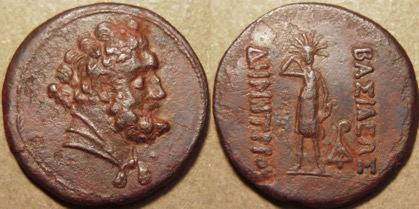
\includegraphics[width=.6\linewidth]{Raza-Figure02}
	\caption{Demetrius I. Bust of Heracles / Artemis with radiate halo. 
		{\normalfont\scriptsize \\ \coinindia}}
	\label{fig:Raza-Figure02}
\end{figure}
%\end{wrapfigure}

The next coin type under discussion is the ‘elephant aegis’.
This refers to an obverse portrait of the monarch wearing an elephant’s head on his left shoulder (see \cref{fig:Raza-Figure03}).
The coin type was issued solely by Lysias (c. 120-110\BC), an Indo-Greek king who ruled in modern Afghanistan and Pakistan \parencite[121]{Mairs2014}.
The design constitutes Lysias’ innovation on a standard obverse type in which Indo-Greek kings wore a protective goatskin aegis bearing the face of Medusa (see \cref{fig:Raza-Figure04}) \parencite[35]{Whitehead1970}.
One reading of the coin type is based on the elephant slayer motif. Lysias was the second king to wear an elephant headdress on coins, and just as with Demetrius I, it has been suggested that his coinage symbolises Indian conquests \parencites[341]{Cribb2011}[107]{Widemann2003}.
Certainly, the coin type represents Lysias in the act of hurling a spear, alluding to the Graeco-Macedonian concept of \emph{doriktetos chora}, ‘by the spear’, meaning the right of rule by conquest \parencite[27]{Billows1995}.
If this reading is correct, Lysias’ elephant head was a symbol of conquest, and not a traditional Greek aegis which imbued the wearer with the protection of Zeus and Athena \parencite[185]{Holt1999}.

\begin{figure}[!htb] %Figure 3
	%\begin{wrapfigure}{O}{0.5\textwidth} 
	\centering
	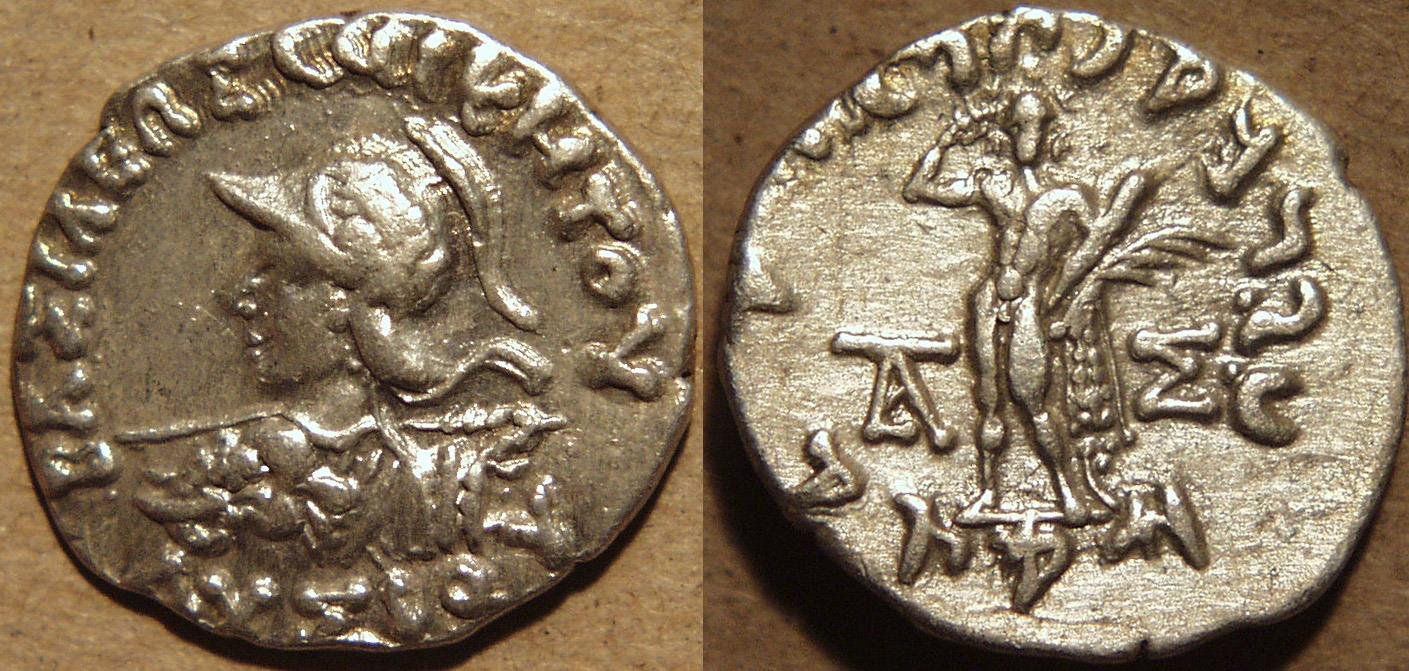
\includegraphics[width=.6\linewidth]{Raza-Figure03}
	\caption{Lysias. King brandishing spear and wearing an elephant’s head with protruding tusks on left shoulder / Heracles holding diadem, club, and lion skin. 
		{\normalfont\scriptsize \\ \coinindia}}
	\label{fig:Raza-Figure03}
\end{figure}
%\end{wrapfigure}

On the other hand, it has been pointed out that Lysias wears the elephant’s head, “as if it belonged to an aegis” \parencite[86]{Bopearachchi1990}.
Furthermore, the kings wearing the goatskin also represented themselves hurling spears, making the spear-thrower motif a general symbol of royal power (see \cref{fig:Raza-Figure04}).
Thus, some suggest that Lysias’ elephant head did constitute an aegis, albeit one that represented him as a warrior-king under the protection of an unspecified ‘Indian elephant deity’ \parencite[35]{Whitehead1970}.
This view holds that there was a divide between Greek and Indian religions, and that Lysias presumably adhered to the ‘elephant party’ of Indo-Greeks that rejected Greek religion, warring with the traditionalists from the ‘Zeus party’ \parencites[94]{Whitehead1970}[26]{Widemann2007}.

\begin{figure}[!htb] %Figure 4
	%\begin{wrapfigure}{O}{0.5\textwidth} 
	\centering
	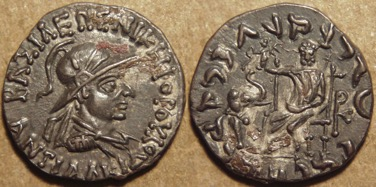
\includegraphics[width=.6\linewidth]{Raza-Figure04}
	\caption{Antialcidas. King brandishing spear and wearing goatskin aegis on left shoulder / Zeus with an elephant. Nike on top of an elephant’s head.
		{\normalfont\scriptsize \\ \coinindia}}
	\label{fig:Raza-Figure04}
\end{figure}
%\end{wrapfigure}
 
Some have emphasised the superficial nature of the ‘elephant party’, suggesting that the force of Lysias’ symbolism lay in its oppositional value \parencite[114]{Widemann2003}.
There had been no intentional concession to Indian cults. Lysias merely subverted a traditional Greek iconographic scheme, and thereby disassociated himself from the ‘Zeus party’, which evidently attempted to enforce Indian worship of Greek gods \parencite[26]{Widemann2007}.
This paper supports the view that Lysias’ elephant’s head represented an aegis meant to imbue the king with divine protection and power.
However, the paper argues against the existence of a gulf between Greek and Indian cults, suggesting that Lysias was expressing his royal power in a cross-cultural context that accommodated both groups.
  
First, Lysias was possibly co-ruler with another Indo-Greek king, Antialcidas (c. 115-95\BC) \parencite[121]{Mairs2014}.
Both were contemporaries who ruled in the roughly same area, and shared monograms – the identifying marks made on coins by minting officials.
This suggests that they both had access to the same mints at the same time.
In addition, Lysias and Antialcidas evidently issued joint coins, which bear legends or inscriptions of both kings.
One coin type features the legend of Lysias on the obverse side, and that of Antialcidas on the reverse, while another reverses the arrangements of the first.
The existence of two antithetical hybrid issues suggests that the coins were part of a deliberate series, and not erroneous issues, as some had supposed before the discovery of the second specimen \parencites[1184]{Bopearachchi2015}[154]{Narain2003}.
If it is accepted that the hybrid coins were jointly issued, Lysias and Antialcidas were probably co-rulers, and their coins cannot be studied without reference to each other.

The significance of Lysias’ association with Antialcidas is that the latter represented the elephant in proximity to Greek divinities.
One reverse design features Zeus, holding a sceptre, and striding beside an elephant. Meanwhile, the goddess Nike, holding a wreath symbolising victory, stands on top of the elephant’s head (see \cref{fig:Raza-Figure04}) \parencite[27]{Narain1991}.
Another reverse design depicts the protome of an elephant, its trunk raised like a salute to the enthroned Zeus.
In turn, Zeus holds a sceptre in one hand and, with the other, supports a wreath-bearing Nike symbolising victory (see \cref{fig:Raza-Figure05}) \parencite[33--34]{Whitehead1970}.
Significantly, the obverse of the first specimen represents Antialcidas in the goatskin aegis eschewed by Lysias.
Antialcidas thus might have been invoking the power and protection of Zeus, who also has the elephant under his aegis on the coins. 

\begin{figure}[!htb] %Figure 5
	%\begin{wrapfigure}{O}{0.5\textwidth} 
	\centering
	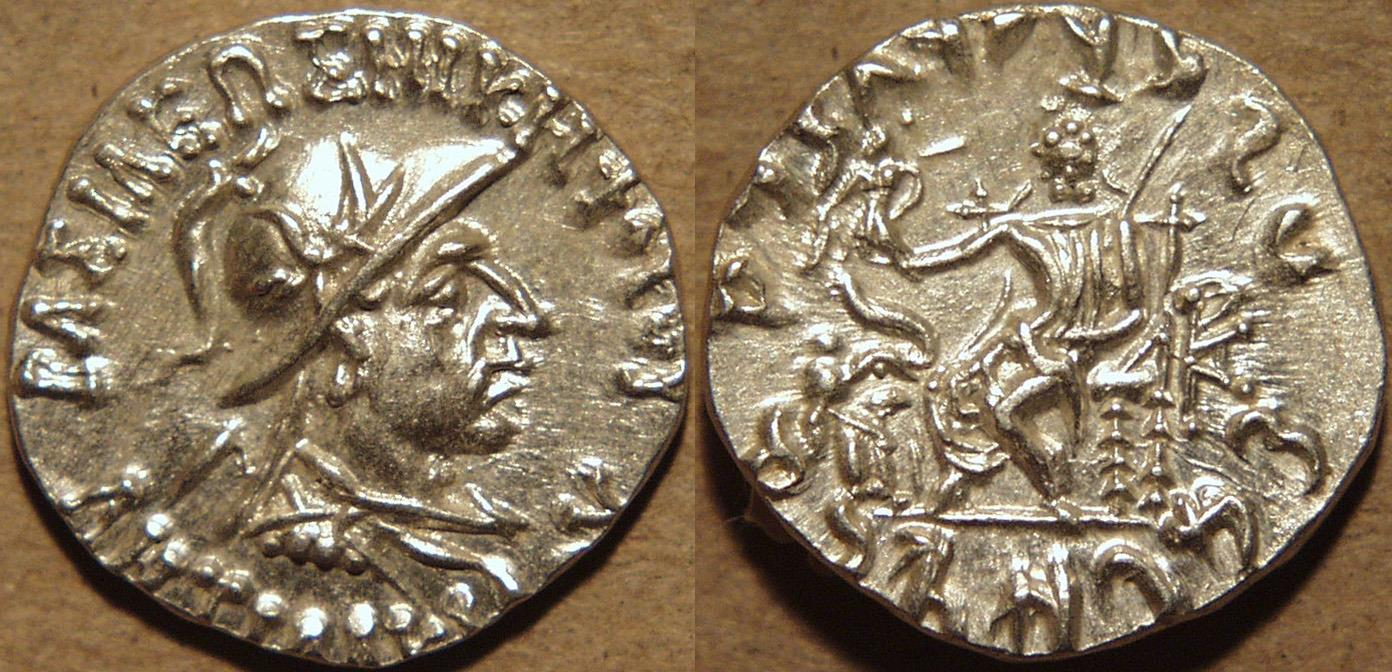
\includegraphics[width=.6\linewidth]{Raza-Figure05}
	\caption{Antialcidas. Portrait of king / Elephant saluting Zeus on throne. Nike in Zeus’ right hand.
		{\normalfont\scriptsize \\ \coinindia}}
	\label{fig:Raza-Figure05}
\end{figure}
%\end{wrapfigure}

If Lysias and Antialcidas were co-rulers, it would be difficult to reconcile the high status accorded to the elephant on the one hand, and the predatory meaning ascribed to the elephant imagery on the other.
Accordingly, it is plausible that Lysias’ elephant’s head represents an innovation on the traditional aegis iconography, rendered in an Indian context with the elephant as a divinising symbol of Zeus.
An elephant’s head was not necessarily an affront to Indians. The elephant head crown of the Pallavas has been noted previously \parencite[66--70]{Hudson2008}. 
Moreover, although the elephant was the sacred animal of Indra, it had been evidently transferred to Zeus.
It is possible that elephant aegis originated as a result.
Notably, the \emph{Vedas} described Indra as being “clothed in might like an elephant”, suggesting a possible Indian tradition accessible to the Greeks and deployed in the context of Zeus \parencite[22]{Gupta1983}. 

In fact, Zeus himself might have been approximated to Indra.
It is suggestive that Antialcidas’ coins represent Zeus wielding a thunderbolt and in proximity to elephants, not unlike Indra’s representation in Indian tradition (see \cref{fig:Raza-Figure04,fig:Raza-Figure05,fig:Raza-Figure06}) \parencite[242--247]{MacDowall2007b}.
Similarly, the Graeco-Bactrian king, Antimachus I (c. 174-165\BC), associated the elephant and the thunderbolt on his coins (see \cref{fig:Raza-Figure07}). 

\begin{figure}[!htb] %Figure 6
	%\begin{wrapfigure}{O}{0.5\textwidth} 
	\centering
	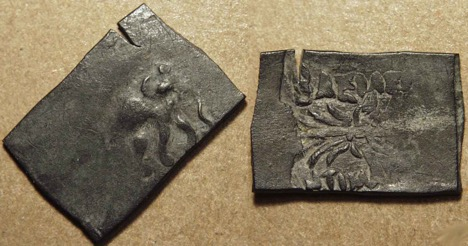
\includegraphics[width=.6\linewidth]{Raza-Figure06}
	\caption{Antialcidas. Zeus holding thunderbolt / Caps and palms of the Dioscuri.
		{\normalfont\scriptsize \\ \coinindia}}
	\label{fig:Raza-Figure06}
\end{figure}
%\end{wrapfigure}

\begin{figure}[!htb] %Figure 7
	%\begin{wrapfigure}{O}{0.5\textwidth} 
	\centering
	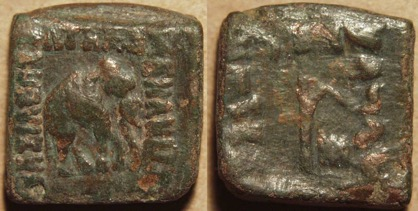
\includegraphics[width=.6\linewidth]{Raza-Figure07}
	\caption{Antimachus I. Elephant walking right / Winged thunderbolt.
		{\normalfont\scriptsize \\ \coinindia}}
	\label{fig:Raza-Figure07}
\end{figure}
%\end{wrapfigure}

Finally, there is the evidence of Heliodorus, the ambassador of Antialcidas to the court of the Indian king, Bhagabadra, in Vidisha.
While in Vidisha, Heliodorus left behind an inscription professing devotion to Vasudeva, a manifestation of the god Vishnu.
Significantly, Heliodorus designated the pillar on which the inscription was written as the ‘Garuda pillar’, alluding to the sacred hawk of Vishnu.
It is thought that the structure was originally topped by a statue of Garuda \parencite[126--127]{Mairs2014}.
Thus, it seems the Indo-Greeks took part in local cults, and were aware of the iconographic schemes of local gods, including possibly the elephant’s proximity to Indra.
Accordingly, Indra might have been worshipped as Zeus, accounting for the Greek aegis rendered in an Indian context.
If so, this suggests a royal conception of power that extended beyond their Greek heritage, incorporating local Indian traditions as well.

The last coin type under discussion is the ‘elephant goad’.
This refers to coins with an elephant on the obverse side and an elephant goad on the reverse – the goad being the tool used by Indian \emph{mahouts} or elephant drivers to train and control the animal (see \cref{fig:Raza-Figure08}).
The coin type was issued by only one Indo-Greek king, Menander I (c. 165/155-135\BC), whose kingdom was centred on the Punjab in modern Pakistan and India.
Menander was an important ruler whose reputation has been preserved in both Indian and classical sources \parencite[14--17]{Bopearachchi1993}.
The Buddhist text \emph{Milindapanha} portrays Menander as a wise Buddhist king who abdicated his throne to retire to an ascetic life \parencite[14--17]{Bopearachchi1993}.
Classical authors provide a different perspective.
Plutarch writes that Menander was celebrated for his rule, but that he died in camp, presumably while on a military campaign.
Strabo adds that Menander was the most successful Indo-Greek general, comparing him to Alexander the Great \parentext{\cite[180--183]{Holt1999}; Strab. Geo. 11.11.1; Plut. Mor. 821d}.

\begin{figure}[!htb] %Figure 8
	%\begin{wrapfigure}{O}{0.5\textwidth} 
	\centering
	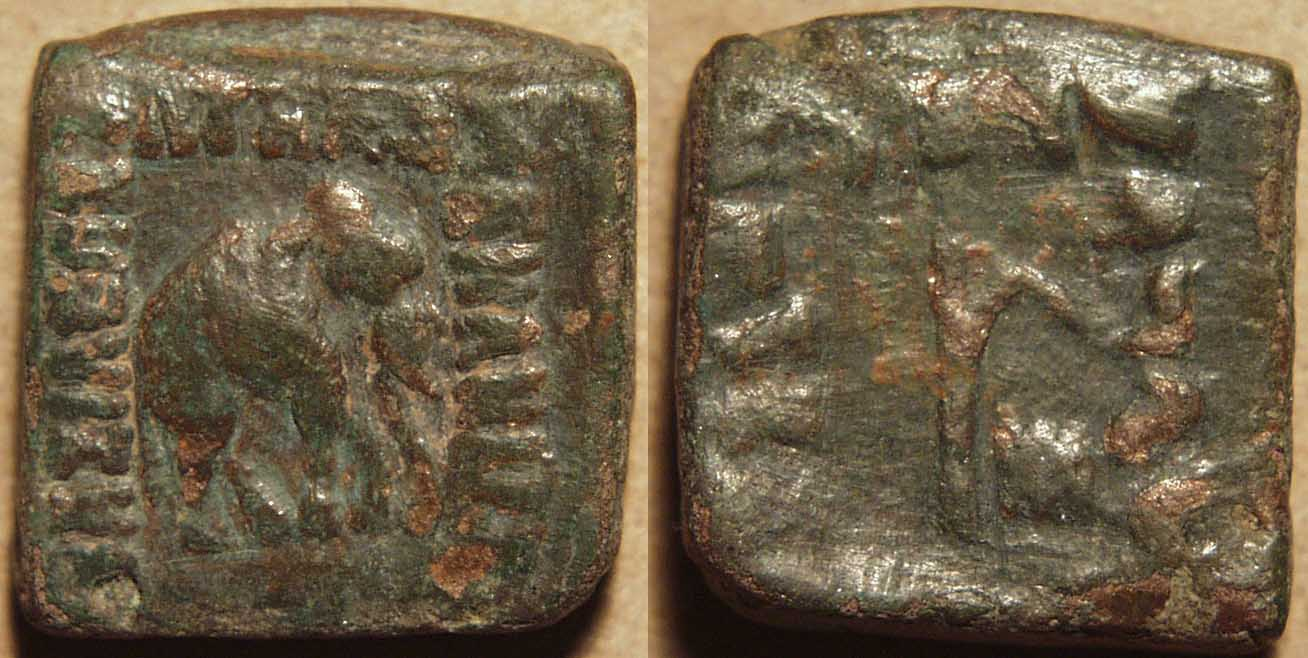
\includegraphics[width=.6\linewidth]{Raza-Figure08}
	\caption{Menander I. Elephant walking right / Elephant goad.
		{\normalfont\scriptsize \\ \coinindia}}
	\label{fig:Raza-Figure08}
\end{figure}
%\end{wrapfigure}

In scholarship, the testimony of the classical authors has been privileged by some, and Menander is considered primarily as a Hellenistic warrior king.
One scholar thus observes that, “true to form” of a Hellenistic king, Menander had died waging war.
Menander is also associated with Eucratides I (c. 170-145\BC),
the Graeco-Bactrian king, who, according to Justin,
had weakened himself through the waging of incessant wars,
but in more cynical translations was said to have “bled Bactria to death”
\parentext{\cites[128]{Holt2005}[156]{Mairs2014}[270]{Tarn1951}; Justin. Ep. 41.6}.
In contrast, Menander’s representation as a philosopher king in the \emph{Milindapanha} has been summarily dismissed as Buddhist missionary ‘propaganda’, which overlooks his actual ‘warlike’ and ‘murderous’ tendencies \parencites[234]{Widemann2000}[15--16]{Widemann2007}.
Accordingly, the elephant and goad on Menander’s coins have been associated with Greek imperialism, presumably representing the Greeks as the masters of elephants, and hence of Indians \parencite[87--89]{Fussman1993}.
This paper argues that this was not necessarily the case and that Menander’s coin type might have represented royal power in a cross-cultural context, accommodating both Greeks and Indians.

While the \emph{Milindapanha} might betray a Buddhist bias, it is suggestive that Menander was considered an ideal figure to represent Indian ideas of kingship.
Significantly, Plutarch writes that after Menander’s death, his subjects competed over his mortal remains and divided them as relics for internment in various monuments.
This calls to mind the division of the Buddha’s ashes in \emph{stupas}, ‘tombs’ set up by his followers, and indicates that Menander might have been honoured by his Indian subjects in the Buddhist fashion \parentext{Plut. Mor. 821d; \cite[145]{Rothkrug2006}}.
Regardless of whether or not Menander was a convert, it seems that Buddhists remembered him with esteem, and honoured him as one of their own \parencite[644]{Mairs2015}.
Thus, Menander might have conceivably reached out to his Indian subjects. The coin type with the elephant and the goad might have been one such instance.

First, elephants had more than just a military role in Indian political tradition.
Owing to their fondness for bathing and the use of the trunk to spray water, elephants became associated with fertility and sky divinities such as Indra, and attributed rainmaking powers \parencite[19]{Gupta1983}.
One origin story was that elephants were clouds cursed to wander among humans, and thus responsible for rainfall when their brethren would bear down on the earth for conjugal visits.
Indian kings were therefore required to maintain royal elephants known as the ‘king’s clouds’ to ensure rainfall for the kingdom’s prosperity.
In fact, elephants were one of the seven \emph{ratnas}, or 'jewels', the necessary symbols of a legitimate Indian monarch \parencites[38--39]{Gonda1966}[107]{Campbell2015}.
As a young ruler, the Buddha charitably gave away the royal elephant to a neighbouring kingdom suffering from drought but, in turn, invited thirst and famine on his own subjects who eventually drove him from his throne \parencite[23--24]{Gupta1983}.
Consequently, the goad might have signified Menander’s possession of elephants, and hence an acknowledgment of his royal duty to maintain the fertility and abundance of the kingdom.

Second, the elephant and goad may have had connotations of justice.
The purposes of the goad were to tame, control, and direct the elephant \parencite[66--67]{Trautmann2015}.
The symbolic nature of the goad as an instrument of control consequently led to its association with law. \emph{Nirankusa}, ‘unrestrained’, the antonym derived from \emph{ankusa}, ‘restrain’, the word for goad in Sanskrit, referred to those who did not follow social norms and rules.
Accordingly, the elephant-headed god Ganesha, who possibly originated during the Indo-Greek period, held the goad as a symbol of his power to restrain the forces of evil \parencites[96]{Alter2004}[144]{Dhavalikar1981}.
Similarly, Buddhist tradition compared the love and wisdom of the Buddha to the goad, capable of taming the wickedness of the elephant Nalagiri \parencite[96]{Dhammika2005}.
Thus, Menander might have been alluding to his role in upholding justice for his subjects, in addition to supporting their welfare.
This reading of the coins would support Menander’s engagement with local traditions and practices of kingship, and possibly account for his reception in Indian tradition.
Notably, Menander did strike coins showing the \emph{chakra}, the ‘wheel’, the symbol par excellence of the \emph{Chakravartin}, the rightful universal monarch of Indian tradition (see \cref{fig:Raza-Figure09}) \parencite[15]{Stanco2012}.

\begin{figure}[!htb] %Figure 9
	%\begin{wrapfigure}{O}{0.5\textwidth} 
	\centering
	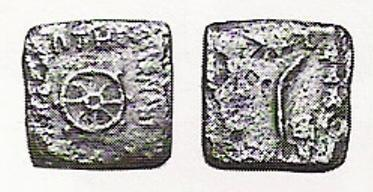
\includegraphics[width=.6\linewidth]{Raza-Figure09}
	\caption{Menander I. Wheel / Palm branch.
		{\normalfont\scriptsize \\ \coinindia}}
	\label{fig:Raza-Figure09}
\end{figure}
%\end{wrapfigure}

Finally, the elephant and goad coins might have represented Menander’s military power, which is emphasised by classical authors \parencite[644]{Mairs2015}.
For the Greeks, a goad represented power over elephants and symbolically alluded to the strength of the wielder.
Alexander had evidently aggrandised his Indian triumphs on the so-called ‘elephant medallion’ coins by representing his defeat of the Indian ruler, Porus, a giant figure controlling an elephant with a goad \parencites[151--152]{Holt2003}[204--205]{Stewart1993}.
While Menander did not represent himself as an elephant tamer per se, the goad might have nevertheless represented royal military power to Greeks, as evident in the king’s possession of powerful war elephants. 

Moreover, the Greek author of the \emph{Periplus Maris Erythrae} reports seeing the coins of Menander in the Indian port of Barygaza (Baruch), and takes special note of the iconography \parentext{PME. 47}.
Conceivably, the author would have interpreted the coins in a Greek context. In contrast, an Indian might have equated the elephant and the goad with local traditions.
The point is that the coin type would have resonated in both a Greek and an Indian context.
Consequently, it would be unjustified to dismiss Menander’s reputation as an Indian philosopher king, and focus on the Hellenistic warrior king found in the classical authors.
Menander could have represented himself as both, appealing to Greeks and Indians.

In conclusion, elephant motifs on Graeco-Bactrian and Indo-Greek coinage legitimised royal authority in a cross-cultural context.
The view that the Graeco-Bactrian and Indo-Greek kings did not engage with local ruling traditions is not borne out by the coins.
The picture that emerges supports the recent literature emphasising the cosmopolitan conception of royal power in the Hellenistic kingdoms \parencite[11]{Strootman2014}.
However, a ‘Hellenocentric’ approach has meant that the cross-cultural significance of the elephant motifs is not fully appreciated.
When studying the coins, scholars should take note to consider not only the Greek context, but also the possible local significance of the iconography.
Through consideration of local contexts, scholars will be able to gain a better understanding of how Hellenistic kings established and maintained their power over diverse, multi-ethnic populations.

\IJSRAseparator
I \IJSRAsection{Acknowledgements} would like to thank the IJSRA editors and Candida Crewe for their assistance and critical comments.
\IJSRAclosing%<<<< DO NOT change this line
\end{document}
\documentclass[english]{ijsra}
\def\IJSRAidentifier{\currfilebase} %<---- don’t change this!
%-------Title | Email | Keywords | Abstract-------------
\def\shorttitle{Heritage in the Context of Nationalism}
\def\maintitle{The Rule of Law and the Power of Suggestion: Heritage in the Context of Nationalism}
\def\cmail{robrownd@gmail.com}
\def\keywords{Preservation, Cultural Heritage, Philippines, UNESCO, World Heritage, nationalism}
%\def\keywordname{}%<--- redefine the name “Keywords“ in needed language
\def\abstract{This \IJSRAsection{Abstract} paper discusses the concept of prehistoric archaeological heritage on a world scale by considering the intentions, functionality and language of the Republic of the Philippines’ Law 10066 (\textit{The National Cultural Heritage Act of 2009}) and the Council of Europe’s Treaty of Valletta (\textit{Convention on the Protection of the Archaeological Heritage, 1992}). Both exist quite comfortably under the umbrella of the current UNESCO World Heritage initiatives. This paper acknowledges the necessity and benefits of Existing Political Units administrating and rationalizing the recovery process of artifacts found within their current borders. It also suggests that heritage law is most easily implemented and most effective when applied to a physical landscape rather than a contemporary political unit such as a nation state. In the case of countries such as the Philippines where the current political boundaries are the same as the boundaries of the physical landscape, a national law or policy is sufficient. In the case of a currently politically divided landscape such as the CoE, a region-wide policy that establishes a common set of standards and expectations as a buffer between the different national governments is a better option.}

%--------Author’s names------------
\def\authorone{Rob Rownd}
%\def\authortwo{}
%-------Biographical information-------------
%\def\bioone{Get author bio}
%\def\biotwo{--}
%------University/Institution--------------
\def\affilone{Graduate Student at the Archaeological Studies Program, University of the Philippines\\ Professor, University of the Philippines’ Film Institute}
%\def\affiltwo{}%<---- comment or delete if there is no second author.
%\def\affilthree{}%<---- comment or delete if there is no third author.
%\def\affilfour{}%<---- comment or delete if there is no fourth author.
%\def\affilfive{}%<---- comment or delete if there is no fifth author.
%--------Mapping of authors to affiliations------------
%% authorone:--> * <--- copy/paste that symbol to \affiloneauthor etc. below
%% authortwo:--> † <--- copy/paste that symbol to \affiloneauthor etc. below
%% authorthree:--> ‡ <--- copy/paste that symbol to \affiloneauthor etc. below
%% authorfour: --> § <--- copy/paste that symbol to \affiloneauthor etc. below
%% authorfive: --> ¶ <--- copy/paste that symbol to \affiloneauthor etc. below
%-------------------------------------------------------------------------
%\def\affiloneauthor{}%<---- paste the symbol of the authors into {}
%\def\affiltwoauthor{}%<---- paste the symbol of the authors into {}
%\def\affilthreeauthor{}%<---- paste the symbol of the authors into {}
%\def\affilfourauthor{}%<---- paste the symbol of the authors into {}
%\def\affilfiveauthor{}%<---- paste the symbol of the authors into {}

\begin{filecontents}{\IJSRAidentifier.bib}

@report{Aleta_2003,
	author = {Aleta, D.G.A. and Tomita, K. and Aleta, J.T. and Lupo, E.S. and Kawano, M.},
	title = {Clay Mineralogical Study of the Pliocene-Pleistocene Carcar Formation and the Quaternar Alluvium in Consolacion-Lilo Cebu Province, Philippines},
	type = {Reports of the Faculty of Science},
	institution = {Kagoshima University},
	date = {2003},
}

@periodical{CoE_2000,
	title = {The official Gazette of the Council of Europe},
	date = {2000},
	publisher = {Council of Europe Publications},
	location = {Strasbourg},
}

@online{CIA_2001,
	title = {Our reply to EH Position Statement},
	date = {2001},
	url = {http://www.independents.org.uk/the-valletta-report/english-heritage-position-statement/our-reply-to-eh-position-statement},
	subtitle = {A reply to the Position Statement},
	organization = {Council for Independent Archaeology },
	urldate = {2015-06-24},
}

@article{Conard_2009,
	author = {Conard, N. and Malina, M and Munzel, S.},
	title = {New flutes document the earliest musical tradition in southwestern Germany},
	journaltitle = {Natuee},
	date = {2009},
	number = {460},
	pages = {737--740},
}

@online{Valletta_1992,
	title = {The Treaty of Valletta},
	date = {1992},
	url = {www.conventions.coe.int/Treaty/EN/Treaties/Html/143.htm},
	organization = {Council of Europe Select Committee of Experts on Archaeology and Planning},
	urldate = {2015-06-20},
}

@online{Divers_2014a,
	title = {Doc’s Cave},
	subtitle = {the Pawod underwater cave system},
	date = {2014},
	url = {https://filipinocavedivers.com/2014/07/26/docboys-cave-aka-the-pawod-underwater-cave-system/},
	organization = {Filipino Cave Divers},
	urldate = {2016-08-20},
}

@online{Divers_2014b,
	title = {Guidelines},
	date = {2014},
	url = {https://filipinocavedivers.com/guidelines/},
	organization = {Filipino Cave Divers},
	urldate = {2016-08-20},
}

@article{Groenewoudt_2014,
	author = {Groenewoudt, B.},
	title = {Valletta Harvest: value for money},
	journaltitle = {EAC Occasional Paper},
	date = {2014},
	num = {10},
}

@online{President_260,
	author = {Marcos, F.},
	title = {Presidential Decree 260},
	date = {1973},
	url = {http://www.gov.ph/1973/08/01/presidential-decree-no-260-s-1973/},
	urldate = {2016-12-05},
}

@online{President_1505,
	author = {Marcos, F.},
	title = {Presidential Decree 1505},
	date = {1978},
	url = {http://www.gov.ph/1978/06/11/presidential-decree-no-1505-s-1978/},
	urldate = {2016-12-05},
}

@online {Potts_2015,
	author = {Potts, L.},
	title  = {Digging for treasure},
	subtitle = {Is 'nighthawking' stealing our past?},
	organization = {BBC News},
	year   = {2015},
	url    = {http://www.bbc.com/news/uk-england-31848684},
	date = {2015-06-23},
}


@online{RA4886,
	organization = {Republic of the Philippines},
	title = {Cultural Properties Preservation and Protection Act},
	subtitle = {RA 4886},
	date = {1966},
	url = {www.philippinelaw.info/statutes/bp4846.htm},
	subtitle = {RA 4886},
}

@online{RA10066,
	organization = {Republic of the Philippines},
	title = {The Philippine Cultural Heritage Act},
	date = {2009},
	url = {http://ncca.gov.ph/republic-act-no-10066/},
	subtitle = {RA 100066},
	urldate = {2015-05-27},
}

@online{Roeher_2006,
	author = {Roeher, F.},
	title  = {Watching the detectorists},
	organization = {BBC News Magazine},
	date   = {2006},
	url    = {http://news.bbc.co.uk/2/hi/uk_news/magazine/4966424.stm},
}

@online{Ta-as_2014,
	author = {Ta-as, A.},
	title = {Mactan Sea Cave Surprise},
	date = {2014},
	url = {http://cebudailynews.inquirer.net/34991/mactan-sea-cave-surprise-doc-amores-pushed-for-marine-sanctuary},
	subtitle = {‘Doc Amores’ pushed for marine sanctuary},
	organization = {Cebu Daily News},
}

@online{Tankersley_2014,
	author = {Tankersley, C.},
	title = {Historical Preservation in the Philippines},
	date = {2014},
	url = {www.preservelaw.com/2014/01/historic-preservation-philippines},
	organization = {Preserve Law: A Cultural Heritage Law Blog},
}

@article{Trotzieg_1995,
	author = {Trotzieg, G.},
	title = {Archaeology as Part of the Swedish Support to Developing Countries},
	journaltitle = {Current Swedish Archaeology},
	date = {1995},
	volume = {3},
}

@online{UNESCO_2003,
	title = {Philippine Cultural Heritage Law},
	date = {2003},
	url = {http://www.unesco.org/culture/natlaws/media/pdf/philippines/ph_backgroundculthrtgelawinstit_engorof.pdf},
	subtitle = {Background},
	organization = {UNESCO},
	urldate = {2015-06-28},
}

@online{Cairo_2015,
	title = {Intangible Cultural Heritage},
	date = {2015},
	url = {www.unesco.org/new/en/cairo/culture/intangible-cultural-heritage/},
	organization = {UNESCO Office in Cairo},
	urldate = {2016-05-25},
}

@article{Willems_2007,
	author = {Willems, W. J. H.},
	title = {The work of making Malta: The Council of Europe’s Archaeology and Planning Committee 1988-1996},
	journaltitle = {European Journal of Archaeology},
	date = {2007},
	volume = {10},
	issue = {1},
	pages = {51--77},
}

@online{Young_2001,
	author = {Young, C.},
	title = {English Heritage Position Statement on the Valletta Convention },
	date = {2001},
	url = {http://www.independents.org.uk/the-valletta-report/english-heritage-position-statement},
	organization = {Council for Independent Archaeology},
}


\end{filecontents}

\begin{document}
%\begin{otherlanguage}{spanish}
\IJSRAopening
%-------
\lettrine{A}{wareness} of the impact of contemporary cultural identities and contemporary notions of cultural difference on archaeological praxis and the concept of ‘heritage’ itself has matured considerably in the last 50 years. Despite this ever increasing self-knowledge, the relationship between the workers in archaeology  doing the digging and the objects being dug up exists in a negotiated, politicized and, therefore, temporary space. As such, heritage will always be subject to reinterpretation. Heritage law is concerned with assigning ownership of objects found \textit{in situ} and then using that sense of ownership to control and track those objects as they move down the modern scientific \textit{chaîne opératoire} towards scholarly publication and public display. Typically, this is accomplished by designating a given government authority the right to control the granting of permissions to look for, excavate, and then, retrieve objects to further study their potential archaeological value.

Republic of the Philippines’ Act 10066 \parencite{RA10066}, and the Council of Europe’s Treaty of Valletta \parencite{Valletta_1992} are the products of two contemporary political units with very different goals. The Philippines is both a young nation and a developing country still in the process of defining itself on its own terms. 
Filipino prehistoric archaeological heritage carries the weight of reaching back past colonial influences to touch something more uniquely or purely Filipino. The Council of Europe (CoE) contains the 28 member states of the European Union (EU) and 19 other countries that can best be described collectively as having a proverbial “\textit{toe hold}” in the European continent. 
These 19 additional countries include 12 states that have recently been part of the Soviet Union or Yugoslavia, the 3 remaining principalities of southern Europe (Andorra, Monaco, and San Marino), Iceland, Norway, Switzerland, and Turkey.  With the exception of a few of the previously communist countries, the CoE is comprised of relatively older nation states with a more established collective sense of their individual national/ethnic identities. Founded in the decade after the Second World War by many of the same countries who would go on to found what became the EU, it is a truly modern assembly that is more organized around common ideas and shared values than a common tradition such as a religion, economy, ethnicity or location. Not surprisingly, describing European prehistoric archaeological heritage carries the weight of reaching back past current political and ethnic divisions to touch something more intrinsically universal (or, at least, more pan-European) in the deep past. 
 
While the ‘science’ from both Europe and the Philippines follows the internal rules of objectivity prescribed by the scientific method, \textit{cultural heritage} is comprised of more than that. Pure or objective findings are always going to be contextualized in a meaning or series of meanings that is not controlled by either scientific institutions or scientists themselves. To put it simply, the residue of the past is always going to be political. This idea of scientific value being wrapped in something less tangible but equally important is at the heart of UNESCO’s Heritage Criteria. Being focused on finding and decoding the material traces of previous cultures, archaeology is a study of physical things. But even our very grounded, very quantifiable, very tangible discipline has expanded to include much fainter traces of the human past. These include such things as “landscapes, industrial remains and other various forms with the notion of World Heritage or heritage common to humankind.  This particularly fragile form of heritage, often under threat of extinction, had not until now enjoyed sufficient sustained attention” \parencite{Cairo_2015}. 

The authors of the above UNESCO quote are specifically referencing the fragility of ‘Intangible Heritage’ such as traditional dance, music and a given culture’s relationship to the landscape. However, for past tangible heritage, the situation can be similarly challenging, as well as rewarding. For example, it is an amazing accomplishment to reconstruct a 30-thousand-year old flute from 12 bone fragments, as excavators led by Nicholas Conard did in Hohle Fels Cave, Germany. Working with a sieve, the bone fragments were collected from half a cubic meter of earth and then, back in the lab, painstakingly reverse jigsawed into a single instrument that makes noises that we easily recognize to be music.  However the sense of wonder such a reconstruction generates soon expands beyond the academic questions about what kind of music was made with it and what purpose(s) it served \parencite{Conard_2009}. 
For the public, there is a real sense of surprise that music (and therefore musicians) and, at other sites, paintings (and therefore painters) have existed for so long. When done well, public archaeology can change the collective understanding of our past by showing us the seeds of our current behavior in unexpected places and times. I would suggest that it is these new conceptual wrappers of the physical objects actually recovered that really capture the public imagination and promote the development of a deeper public understanding of who we are and what we do as a species. The realization that people have been doing the same things we do now for a very long time changes the questions we ask about ourselves in the past and in the present. 

\IJSRAsection{Multiple levels of Public Policy moving toward a Common Goal}

Despite the significant differences between the drafting bodies and the contemporary contexts, Philippine and Council of Europe heritage policies are quite similar on a functional level. The published planning documents for both of them tacitly acknowledge a common problem: private individuals removing artifacts from the ground and selling them to private collectors without allowing the public, including scientists, to be made aware of them, let alone study them \parencites[2]{Valletta_1992}[18-20]{RA10066}. To combat this, heritage law moves artifacts into the public space before they are discovered and declares that the public or common right to know, to appreciate, and, to understand our past supersedes desires for private ownership. Because these two policies were written by different types of agencies, (one a National government and one a Regional/International ‘authority’), they differ in tone while agreeing on this common goal and method. 

\IJSRAsection{Heritage on a National Level: The Philippines}

RA10066 bluntly assigns ownership of the moveable physical objects found in the ground within the borders of the country to the State. While RA100066 acknowledges private ownership of land and immobile structures on that land, even those considered to be \textit{cultural properties} and \textit{National Treasures}, it clearly separates ‘moveable objects’ from these “immovable cultural properties” \parencite{RA10066} and assigns their administration solely to the National Museum. Because there are currently no known ‘permanent structures’ considered to be prehistoric in the Philippines, the National Museum has effectively been assigned all authority over pre-historic sites and objects in the country including the ability to directly deputize the Armed Forces of the Philippines, the National Police and other local and national investigative agencies to enforce the act. 

This inclusive document is boilerplate legal writing that simply and clearly defines relevant terms, delegates authority and establishes processes \textit{including the legal penalties} to be doled out to violators. 
It is also a solidly nationalistic law that moves the decision-making power over sites and artifacts away from the Local Government Organization (LGO) of an area and gives it to the National Museum. While in practice this consolidation of authority has frequently created administrative bottlenecks for archaeological workers, it is a necessary rationalization of the overall heritage process because it creates an easily understood framework that clearly assigns accountability for any phase of the process including any ‘accidental’ discoveries of artifacts and sites \parencite[8]{RA10066}.

As a final point, it is worth observing how RA10066 moves heritage away from all elected officials and into the hands of professionals and specialists.  In an excellent case study written last year, American cultural heritage lawyer Clinton Tankersley traces the development of Philippines Heritage legislation from the early days of the American Occupation Period onwards. American Commission Act No. 243, passed in 1901, mandated the installation of the Rizal Monument on the Luneta in Manila \parencite{Tankersley_2014}. 
It was the first time any government agency had issued a heritage decree of any kind in the country.  For the next 64 years, in both the Commonwealth and then the Republic, heritage legislation can best be described as a piece-by-piece and almost backhanded expansion of the concept of eminent domain into Philippine public space. The Philippines Historical Research and Markers Committee had its name shortened to the Philippines Historical Committee in 1937 but was never granted the authority to do more than identify sites of historical significance with a plaque and a speech. Even with the Cultural Properties Preservation and Protection Act of 1965 \parencite{RA4886} creating a new category of Object, ‘the Cultural Treasure’ and formally declaring that the government would “preserve and protect the cultural properties of the nation” \parencite[1]{RA4886}, 
the government only allowed itself the right to comment on a privately held ‘cultural treasure’ when it was being sold or going to be sent abroad for exhibition or study. When dealing with prehistoric material, the act only gave the Government the ability to require: 1) permits for excavation and; 2) permits for artifacts to leave the country but no power to police or track their movements within the country \parencite[3]{RA4886} Furthermore, while the CPPPA allowed for methodical cataloging, it was extremely limited and fuzzy in its classification system. 
For example, the act significantly limited the number of possible ‘Cultural Treasures’ by declaring that, “[of] each kind or class of objects, only type and five best duplicates may be designated as ‘cultural treasures’. The remainder, if any, shall be treated as cultural property” \parencite[6]{RA4886}. The significance of this is not only the limited number of samples provided with the full protection of the law but also that the act itself required almost instant classification of objects for the preservation protection to take effect. This is almost the opposite of a contemporary accessioning process where almost everything potentially interesting is returned to the lab for further study and clarification. The CPPPA was, in essence, an inventory control system but it was hardly scientific in its methodology.

Still, the CPPPA was a significant improvement over the legislation that existed before it. Ferdinand Marcos receives some credit as the father of Philippine historical preservation because he sponsored it and later added two presidential decrees \parencites{President_260}{President_1505} to fill in some of its loopholes. 
The most significant impact of the presidential decrees forbids the modification or destruction of any identified “important historical edifice” without prior written permission \parencite[2]{Tankersley_2014}. 
But on the whole and compared to RA10066, the Marcos-era declarations are murky and ad hoc at best. For example, final authority for declaring whether an item was a regulated ‘Cultural Treasure’ or simply considered a ‘Cultural Property’, rested with a committee that consisted of the Director of the National Museum, the President of the Republic and two ‘experts’ appointed by the President. 

Whatever the reader’s opinion of Marcos as a leader may be, he was an elected official rather than an independent historian or scientist. Allowing him, or any other elected official to appoint the ‘experts’ who defined the ‘nature’ or value of a particular item kept the whole heritage process squarely in the short term political realm of a given administration.  This structure did not allow the process to develop any semblance of autonomy. As with most things during the Marcos-era, the CPPPA was too tightly controlled and too personalized to be impartial, flexible or, ultimately truly effective. By contrast, RA10066 is a catchall document that only provides the frameworks, definitions, and processes needed to create a fair, efficient, impartial system that is flexible enough to adapt to change. There is no mention of specific scientific or classification methods and the deliberate exclusion of that level of detail allows the intent of the law to be adapted to changes and refinements of those methods as they occur over time. It is a step back from charismatic, situational decision-making and a step towards a more impartial professionalism and transparency.

To date (August 31, 2016), this fresh legislation has not been tested in a court of law. However, in the five and half years since it took effect, RA10066 has been used by both the state and private organizations to begin to claim the idea of a common national heritage (both intangible and solid) that should supersede notions of private interests and personal ownership. Signed into law in March 2010 and broken down into an Implementation document (the working papers used by lawyers and administrators) in 2012, RA10066 is now being used to confront and contain existing violations of common heritage as they happen. Sometimes this involves creating a separation from open-access public land and a place where access is restricted because of the fragility of the heritage elements found there. For example, the private group, Filipino Cave Divers (FDC) began to promote the new law as a way to protect a freshwater cave system that was discovered in the heart of an Industrial Development Zone on Mactan Island in 2002 \parencite{Divers_2014a}. 

\IJSRAsection{Unexpected Purity: A Surprise Find on Mactan Island}

Mactan is a \SI{75}{\kilo\metre\squared} island with a population of \num{430000}, a large international airport and a bustling, tax-incentive driven manufacturing district. It is located just a few kilometers off the shore of the second largest metropolis in the country, Cebu City. 
It is also an uplifted chunk of Karstic limestone that was probably formed in a shallow sea sometime during the late Pliocene to early Pleistocene \parencite{Aleta_2003}. With discovery of the Pawod Underwater Cave System in 2002, modern life and geological time converged a few meters off a road that will take you past Lapu-Lapu City Hall in less than 30 minutes.

Beside the road is a cenote about one third of the size of a basketball court that has been used as a recreational swimming hole as long as people can remember. The freshwater is still reasonably clean but far past drinkable and the rocks surrounding what was a hole in a cave roof are littered with plastic bags, styrofoam takeout containers and other detritus of modern convenience living. One gets the sense that many people have enjoyed themselves here without giving any thought to who owns the land and pool or who takes care of them. This fallow land looks like a vacant lot in need of a good cleaning but there are quite a few undefined spaces like it in the Philippines and they tend to blend together after a while. 

Behind this picnic area, and out of the afternoon sun, is a smaller pool that doesn’t get as much foot traffic.  In 2001, at the bottom of this pool, Dr. Alphonso Amores found a chute that lead to an unknown, pristine, submerged cavern system that is (currently), “the only [known] freshwater underwater cave system in an urban setting” \parencite{Ta-as_2014}. 
Doc boy, as he was known, was a FilAm (Filipino American) retired reconstructive surgeon and avid scuba diver who learned to cave dive in Florida. Coming home to Philippines after retiring, the good doctor discovered the Pawod Cave System and was a founding member of the private group Filipino Cave Divers (FCD) that now uses it as a training ground for new cave divers \parencite{Divers_2014b}. 

Cave diving is an extremely dangerous and technically demanding activity, so it’s not surprising that it appeals to very meticulous, patient people who pay great attention to details. Indeed, the online roster of the FCD is full of scientists, cinematographers, and training directors who had already amassed a slew of advanced diving certifications before they entered a wet cave. One detail that has not escaped their attention is the gradual infiltration of the residue of the less structured human activity in larger pool into the previously untouched environment of the cave. Plastic and other detritus have been found a full \SI{5}{\metre} inside the chute and divers, unaffiliated with the FCD, have damaged the walls of the cave by dragging cinderblocks into the cavern to use as anchors for guidelines \parencite{Divers_2014a}.

The FCD seeks to protect this pristine environment from further abuse by promoting the idea of responsible use or stewardship:

\begin{displayquote}
	Stewardship comes with the privilege of diving the underwater caves. The environment is fragile at best. Guidelines are established and laws are promulgated in order to preserve these unique natural resources \parencite{Divers_2014b}.
\end{displayquote}

In a coordinated campaign to heighten awareness of this fragile site located just a few meters away from a publically used swimming hole and to establish the legality of their own activities within the space, the FCD are lobbying the local municipal government to consolidate existing environmental regulations under the umbrella of RA10066. First, the FCD documented the presence of a significant number of both fresh and saltwater marine fossils and identified some possible geological clues to the origins of Mactan Island in the caves. Then,  armed with these finds the FCD began evoking the archaeological, cultural heritage zone and systemic research into natural history sections of RA10066 to define the Pawod Cave System as an area to be treated differently than the unregulated public pool above it \parencite{Divers_2014b}.

As a developing nation that has only had two-three generations to get used to the idea of actually owning its own land, trying to declare any resources, even those as unique as the Pawod Cave System off limits to unregulated use is very problematic. The sense of squatting or temporarily using something or someplace that will ultimately be taken away from you works against the idea of responsible use or stewardship. The FDC’s creative use of RA10066 as an organizing or consolidating structure to create a sense of common heritage is a work in progress and it is still unknown how successful it will ultimately be.

\IJSRAsection{Heritage on a Regional Level: The Council of Europe}

While RA10066 is a law, a document generated by the state that is able to define and even dictate behavior to institutions and individuals, the Treaty of Valletta is an agreement between established equals (the individual nation states) who share common goals but use different established methods and practices to achieve them. The Treaty is a beautifully written piece of hopeful diplomacy that reflects this. It has to be because there is no mechanism for the CoE to enforce compliance. The CoE is only effective when it convinces nations to willingly adhere to its treaties and enforce them within their own borders at their own expense. It accomplishes this through treaties that constantly remind all involved of their common interests and values while acknowledging their differing methods of pursuing those values and pointing out the potential benefits of continuing peaceful collaboration. Still, it is unfair to label the CoE as simply a Public Relations machine or suggest that it is toothless. Despite lacking an equivalent of the UN’s blue helmeted peacekeeping forces, it has been extremely effective at promoting its agreed upon values and goals simply by monitoring member states compliance with its treaties.   

It is worth remembering at this point that the 1980s and 1990s were a very positive time for the EU. The political unit changed its name twice: first, from the Common Market to The European Community, and then, to the European Union (EU). Each one of these name changes reflected further quantifiable integration of its Labor Markets, Currencies and Industrial Systems. It became easier and easier for people and money to move about within its borders. Today when it comes to commerce, those internal borders have all but disappeared. However, the European Union is expressly forbidden from extending itself into the area of cultural affairs by its founding document, the Treaty of Rome. While the more inclusive CoE is a completely separate entity, some of the original EU member states remain the core of CoE and continue to provide a majority of its funding \parencite[74]{CoE_2000}. 
Whether this is a sinister arrangement or a pragmatic arrangement is a matter of ideological debate irrelevant to this paper but it is certainly clear that a pattern of mutual beneficence and common interests has been followed over the last five decades. The CoE tends to push forward the cultural side of the EU’s economic agenda. It promotes international integration and seeks to establish Council-wide standards for individual rights and responsibilities. With archaeology, the CoE began to standardize the goals and outputs of the discipline by defining a common meaning of Cultural Heritage for its members. The Valletta Treaty of 1992 is the culmination of a 30 year dialog between interested parties. It is the third, and at this point, latest revision of those agreed upon definitions and goals \parencite{Valletta_1992}. 

While RA10066 focuses on definitions, conditions and processes, Valletta focuses on the definitions and intentions that lie underneath them. However, just like RA10066, there is little to no discussion of the details of any method that will be used in preservation work or scientific excavation and research. Instead, those methods are to be determined by the individual nation states who sign the document and agree to collaborate. It is stated that each country involved has the right to use whatever methods they see fit provided that they comply with the sense of common ownership and responsible behavior the treaty is espousing. The specifics of archaeological praxis are just not discussed and, as with RA10066, this allows the document to be more flexible and effective. 

Two clear examples of this can be found in the First and Eighth Articles of the Treaty (\textit{italics mine}): 

\begin{displayquote}
	Article 1- \textit{Definition of the archaeological heritage}
	\begin{enumerate}
		\item The aim of this (revised) Convention is to protect the archaeological heritage as a source of the \textit{European collective memory} and as an instrument for historical and scientific study.
		\item To this end, {the following} shall be considered to be elements of the archaeological heritage, all remains and objects and any other traces of mankind from past epochs:
		\begin{enumerate}
			\item \textit{the preservation and study of which help to retrace the history of mankind and its relation with the natural environment};
			\item for which excavations or discoveries and other methods of research into mankind and the related environment are the main sources of information; and
			\item which are located in any area within the jurisdiction of the Parties. \parencite[2]{Valletta_1992}
		\end{enumerate}
	\end{enumerate}
	Article 8- \{\textit{Promise to Collaborate and Openly Publish}\}\\
	Each Party undertakes:
	\begin{enumerate}
		\item to facilitate the national and international exchange of elements of the archaeological heritage for professional scientific purposes while taking appropriate steps to ensure that such circulation in no way prejudices the cultural and scientific value of those elements;
		\item to promote the pooling of information on archaeological research and excavations in progress and to contribute to the organization of international research programs. \parencite[4]{Valletta_1992}
	\end{enumerate}
\end{displayquote}

Notice that each of these articles is worded in a way that promotes the idea that this is a newly defined common meaning for heritage which does not impinge on or threaten a member nation’s sovereignty over its own past or its current sense of identity. Instead, archaeological heritage found anywhere in Europe is (also) a “source of the European collective memory” and “the preservation and study of which help to retrace the history of mankind and its relation with the natural environment” \parencite[4]{Valletta_1992}. 
The matter-of-fact rhetoric of this treaty is a combination of low key common sense and objective idealism that extends to Article 8’s discussion of collaboration. Here again the simple premise presented is that the heritage belongs equally to everyone collaborating (aka anyone agreeing to follow the treaty) and everyone who signs on the dotted line should have equal access to all of it. All in, for a degree bearing professional archaeology worker, there is little to take issue with in the Valletta Treaty. It is comprised of one common sense idea after another. In an article written tens of years after the treaty was approved, Professor Willem Willems who served as the Dutch representative to the treaties council of Experts between 1988 and 1996, is critical of some aspects of the treaty’s implementation but stresses that:

\begin{displayquote}
	We can be quite certain that the adoption, at Malta, of the Valletta Convention will, in future, be considered to have been a watershed in the development of European archaeology. The Valletta Convention defines a standard for the way in which European states \textit{should} manage their archaeological heritage and also provides a frame of reference in this regard for countries outside Europe. It has placed archaeology – \textit{which used to be, in the main, an academic discipline} – firmly {\textit{and pragmatically}} in the world of spatial planning, contracting and public decision-making, \textit{unsurprisingly to the distress of some of its practitioners} \parencite{Willems_2007}.
\end{displayquote}

Willems’ article is written from the point of view of a true insider connected to both academia and government. In addition to being an established scientist, he has been a university dean, a government official in The Netherlands and served as the president of the European Archaeological Association and other International Organizations. The last sentence in the quote above suggests that in his activist agenda, archaeology and heritage should be more than merely academic concerns. As such, they are best served by practitioners who proactively engage with developers and elected officials. Willems concludes the article with the observation that the ideals of the Valletta agreement would be better served if the EU itself were to agree to the Convention (the Treaty) because the discipline of archaeology would then have a voice in both the EU government and the CoE. While that would very likely be a benefit to archaeology and heritage in the region, it seems extremely unlikely that there would be that significant a change in the constitution of the EU any time. As we can appreciate in the two final examples below, while the member states of the EU share a common economic system, they still have significant cultural differences.  

\IJSRAsection{Information Overload: The Netherlands}

In any case, Valletta has been very effective in influencing archaeological policy and law in the CoE member states, but the degree of effectiveness has varied considerably from state to state. The degree of effectiveness seems to be directly proportional to the length of time the member nation took to ratify the treaty. Willems’ home country of Holland, for example, was an early adopter of the Treaty. Altogether, 20 of the then 43 CoE member nations signed the document within a year and implemented laws that followed its guidelines within two \parencite[58]{Willems_2007}. 
In the 13 years since ratification, Dutch developers have been so compliant with laws based on the models in Valletta that academic archaeologists in Holland are suffering from the happy problem of having to wade through piles and piles of field reports from excavations that were legally required but not motivated by a research question. This inversion of the traditional archaeological process left the Dutch with over \num{7000} site reports of varying quality to mine for data to turn into knowledge. Even with over half of these reports (\num{4000}) being dismissed due to methodological and/or technical issues, the sheer volume of synthesizing work proved to be too much for universities to handle by themselves. 
Given the availability of ample sources of public funding, the demand for the synthesizing services has led to an unusual situation where there are now more archaeologists with PhDs working outside the academic realm of the Netherlands than inside it \parencite[93]{Groenewoudt_2014}.  

This brave new world in which field work and initial data consolidation now came before the developing of research questions created an interesting dynamic. Dutch Heritage (DH) now had to source an enormous volume of work to a mixed field of qualified vendors both inside and outside of academia. This eventually forced (DH) to develop a new process that is more similar to bidding out creative work or even crowd sourcing than it is to traditional academic inquiry. DH solved this by ranking all of the reports based on location, quality of fieldwork and which potential research questions were most likely to be fully or partially answered by synthesizing the research. Universities, private archaeological firms and municipal archaeological services then bid the work on a ‘per project basis’ in the form of a brief that lists price, schedule and personnel to be involved including project leaders. 
The first batch of contracts were awarded in 2013 based on the ‘best’ bid for a given question with the potential quality of the finished work considered more important than price. This first round of ‘contracts’ will be completed in 2016 in the form of dissertations and published academic articles. DH is already happy enough with the preliminary submissions that they plan to continue the program by offering a new round of contracts for bidding in 2015 \parencite{Groenewoudt_2014}. 
It is highly unlikely that anybody foresaw this sudden bonanza of unfocused field data as a byproduct of adopting the models in the Valletta Treaty. Its will be interesting to see how good the science that comes out will be. 

\IJSRAsection{Resistance to Professionalization: England}

While the Netherlands actively embraced Valletta from the start and incorporated its ideas into its scientific processes and legal system, the British were far more reserved and did not implement the Treaty until 2001. According to both Willems and a British organization that calls itself Council for Independent Archeologists, the main sticking point and cause for this delay was the inclusion of Article 3 of the Treaty (\textit{italics mine}) \parencites[62]{Willems_2007}{CIA_2001}. 

\begin{displayquote}
	Article 3\\
	To preserve the archaeological heritage and guarantee the scientific significance of archaeological research work, each Party undertakes:
	\begin{enumerate}
		\item to apply procedures for the \textit{authorization and supervision of excavation} and other archaeological activities in such a way as:  
		\begin{enumerate}
			\item to prevent any illicit excavation or removal of elements of the archaeological heritage; 
			\item to ensure that \textit{archaeological excavations and prospecting are undertaken in a scientific manner} and provided that:
			\begin{enumerate}
				\item non-destructive methods of investigation are applied wherever possible;
				\item the elements of the archaeological heritage are not uncovered or left exposed during or after excavation without provision being made for their proper preservation, conservation and management
			\end{enumerate}
		\end{enumerate}
		\item to ensure that excavations and other potentially destructive techniques are carried out \textit{only by qualified, specially authorized persons}; \parencite{CIA_2001}
	\end{enumerate}
\end{displayquote}


Willems, like all academic archaeologists, lives in a world where archaeology and cultural heritage have the potential to increase knowledge and improve our understanding of ourselves. But he is also part of a select club that actively excludes others. The Valletta Treaty, and RA10066, are both documents that reinforce that exclusion. While they are precise and candid about heritage being publicly owned and emphasize the public’s right to view and understand it, they also actively restrict the role the public is allowed to play in all phases of the process aside from spectatorship.  Both of the documents share a common premise that archaeology is a true profession which requires organized training, peer certification, and government authorizations to control survey work, excavations and the recovery of artifacts. In this world there is no place for the careful and enthusiastic but uncertified amateur aside from volunteering to work on an authorized and supervised dig. Most of the world agrees with them. But, not some of the British.

Amateur archaeology has a long and productive tradition throughout the UK. The British Museum in particular and the academic units of the discipline in general have benefited from some extraordinary finds by amateurs and have learned to live with some of the sloppy documentation and technique to preserve the greater good which came from having a no cost work force scouting for sites to share. Currently there are dozens of active self-proclaimed Amateur Archaeological Societies and an estimated \num{30000} metal detectorists spread throughout the UK \parencites{Roeher_2006}{Potts_2015}. 
While metal detectors are a technology developed to locate bombs during WW2, the roots of some of the societies stretch back to a time well before Mortimer Wheeler. Quite a few of both have absolutely no interest in being supervised by anybody. This is not to suggest that any of them have illicit intentions or are even in it for more than the thrill of the find. Instead, they were and still are true amateurs who do archaeology in their spare time because they love doing it. The problem with the introduction of the Valletta treaty was that their view of both archaeology and heritage was at odds with the more professional science that was supplanting them. Back on the continent, metal detectorists were perceived as a curious and backward lot. That the gentle language of Article 3 would offend them as it did was a complete surprise to the Valletta’s committee of experts because most of the delegates had wanted to include a statement in Article 3 to directly, “ban the unlicensed use of metal detectors” period and only agreed to present what they considered watered down text when the British representative to the committee, trained archaeologist Geoff Wainwright convinced them that the ban would never been accepted in the UK \parencite[62]{Willems_2007}. 

Even after the 8 year lapse that occurred before English Heritage sanctioned the Treaty, the British amateurs were perfectly willing to tell the politicians and university professors exactly where they thought they were wrong. And nearly 25 years after that, the UK is the sole CoE member state that has struck a working truce with its collection of feisty amateurs rather than move on to a purely professionalized work mode. In recent years, this truce has begun to work for the British Governments benefit as dedicated amateurs, especially metal detectorists, have evolved into an amateur policing and early warning system constantly on the lookout for nighthawks (the British version of professional treasure hunters) operating on private and public lands. 

Yet, however happy and functional this resolution is, it is nearly the opposite of the situation that has evolved 300 kilometers further east in The Netherlands. As such it is the best argument for an informal buffer such as the CoE’s Valletta Treaty between nations with different internal politics rather than a common set of binding laws. 

\IJSRAsection{Conclusions}

While profit driven thieves such as the treasure hunters of the Philippines and nighthawks in the UK are a serious problem and most places with a rich archaeological heritage are suffering from one or another form of organized criminal pilfering, the importance of preserving the physical traces of our collective memory and studying them to learn about our species is beginning to become apparent to most people. Both the ‘Rule of Law’ \parencite{RA10066} and the ‘Power of Suggestion’ \parencite{Valletta_1992} are proving to be useful tools for the preservation of cultural heritage. By creating a space to preserve archaeological data, the concept of heritage also creates a context for it to be more deeply respected and understood. With our postmodern mindsets, we would not dare to claim to have created the only context for anything that comes out of the ground. Multiple meanings, contradictory or not, and multiple values are an accepted part of our everyday professional lives as they are an accepted part of our everyday social lives, gradually growing the idea of how interconnected all humans are through identifying, studying and presenting our common heritage.


%\IJSRAsection{small headline}

%\IJSRAseparator


\IJSRAclosing
%\end{otherlanguage}
\end{document}
\documentclass[%
	%draft
	]{ijsra}
\def\IJSRAidentifier{\currfilebase} %<---- don’t change this!
%-------Title | Email | Keywords | Abstract-------------
\def\shorttitle{Gods, Games, and Geography}
\def\maintitle{Gods, Games, and Geography: A Cross Cultural Study of Chance Games and Religious Ideology}
\def\cmail{ddavis17@binghamton.edu}
\def\keywords{cross-cultural studies, anthropology, games of chance, religion, geography, spatial analysis}
%\def\keywordname{}%<--- redefine the name “Keywords“ in needed language
\def\abstract{Previously, cross-cultural studies have been limited by an immense, but largely inaccessible, volume of literature, most of which was not easily comparable to other studies. Recently, with the advent of D-PLACE (a global database of cultural, linguistic, and environmental data), cross-cultural analyses can be conducted between over \num{1400} different cultural groups with relative ease. Utilising this new database, a re-examination of the revolutionary article by Roberts and collegues\footcite{roberts1959} is undertaken, specifically to address the hypothesis that games of chance are more prevalent in cultural groups with “benevolent” gods. Additionally, variables of political integration, mean community population size, geographic location, and the belief in trance states and possession are incorporated to explore correlations between game type presence and religious differences. A total of 377 different cultures are compared in this study, making this the largest sample size used to re-evaluate the \citetitle{roberts1959} hypotheses. Games are abundant in the archaeological record, and provide much detail regarding cultural, religious, and social characteristics of different groups. Thus, this study not only holds anthropological merit, but also benefits the archaeological community.}
%--------Author’s names------------
\def\authorone{Dylan Davis}
%-------Biographical information-------------
\def\bioone{Dylan Davis attends Binghamton University in the United States. He is currently enrolled in a combined Master’s program in anthropology and is also earning a BA Geography, specializing computer applications in human environmental analysis. Dylan’s archaeological interests include human-environmental interactions and their relation to societal development, as well as the incorporation of geographic-techniques for archaeological analyses. He will be focusing his MA thesis on the use of spatial analysis and remote sensing technologies to identify archaeological objects through the use of LiDAR and satellite imagery.}
%------University/Institution--------------
\def\affilone{Binghamton University}



\begin{filecontents}{\IJSRAidentifier.bib}

@ARTICLE {ball1972,
	author  = "Ball, Donald W",
	title   = {The Scaling of Gaming},
	subtitle = {Skill, Strategy, and Chance},
	journal = "The Pacific Sociological Review",
	year    = "1972",
	volume  = "15",
	number  = "3",
	pages   = "277--294"
}

@ARTICLE {barry1980,
	author  = "Barry, Herbert",
	title   = "Ethnographic Atlas XXVIII",
	journal = "Ethnology",
	year    = "1980",
	volume  = "19",
	number  = "2",
	pages   = "245--263"
}

@BOOK {bell1992,
	author    = "Bell, Catherine",
	title     = "Ritual theory, ritual practice",
	publisher = "Oxford University Press",
	year      = "1992",
	location   = "New York"
}

@ARTICLE {binde2005,
	author  = "Binde, Per",
	title   = "Gambling Across Cultures: Mapping Worldwide Occurrence and Learning from Ethnographic Comparison",
	journal = "International Gambling Studies",
	year    = "2005",
	volume  = "5",
	number  = "1",
	pages   = "1--27"
}

@ARTICLE {binde2007,
	author  = "Binde, Per",
	title   = "Gambling and religion: Histories of concord and conflict",
	journal = "Journal of Gambling Issues",
	year    = "2007",
	volume  = "20",
	pages   = "145--165"
}

@ARTICLE {bondarenko2005,
	author  = "Bondarenko, Dmitri and Alexander Kazankov and Daria Khaltourina and Andrey Korotayev",
	title   = {Ethnographic atlas XXXI},
	subtitle = {Peoples of easternmost Europe},
	journal = "Ethnology",
	year    = "2005",
	volume  = "44",
	number  = "3",
	pages   = "261--289"
}

@ARTICLE {botero2014,
	author  = "Botero, Carlos A. and  Beth Gardner and Kirby,Kathryn R.  and Joseph Bulbulia and Gavin,Michael C.  and Gray,Russell D.",
	title   = "The ecology of religious beliefs",
	journal = "Proceedings of the National Academy of Sciences",
	year    = "2014",
	volume  = "111",
	number  = "47",
	pages   = "16784--16789"
}

@ARTICLE {chick1984,
	author  = "Chick, Garry E.",
	title   = "The Cross-Cultural Study of Games",
	journal = "Exercise and Sport Sciences Reviews",
	year    = "1984",
	volume  = "12",
	pages   = "307--337"
}

@ARTICLE {chick1998,
	author  = "Chick, Garry E.",
	title   = {Games in Culture Revisited},
	subtitle ={A Replication and Extension of Roberts, Arth, and Bush (1959)},
	journal = "Cross-Cultural Research",
	year    = "1998",
	volume  = "32",
	number  = "2",
	pages   = "185--206"
}

@INCOLLECTION {chick2015,
	author  = "Chick, Garry E.",
	title     = "Games and Sports",
	booktitle = "Explaining Human Culture",
	publisher = "Human Relations Area Files",
	year      = "2015",
	editor    = "C. R. Ember",
	url     = {http://hraf.yale.edu/ehc/summaries/ games-and-sports},
	urldate = {2016-07-14},
}

@ARTICLE {crist2016,
	author  = "Crist, Walter and de Voogt,Alex  and Dunn-Vaturi,Anne-Elizabeth",
	title   = {Facilitating Interaction},
	subtitle = {Board Games as Social Lubricants in the Ancient Near East},
	journal = "Oxford Journal of Archaeology",
	year    = "2016",
	volume  = "35",
	number  = "2",
	pages   = "179--196"
}

@ARTICLE {davis,
	author  = "Davis, Dylan S.",
	title   = "The Power of Ideology: Religion and Environmental Sustainability in Prehistoric Societies",
	journal = "Nexus: The Canadian Student Journal of Anthropology",
	pubstate    = {inpress},
	volume  = "24",
	number  = "1"
}

@ARTICLE {devoogt2013,
	author  = "de Voogt, Alex and  Dunn-Vaturi,Anne-Elizabeth and Eerkens,Jelmer W.",
	title   = {Cultural transmission in the ancient Near East},
	subtitle = {Twenty squares and fifty-eight holes},
	journal = "Journal of Archaeological Science",
	year    = "2013",
	volume  = "40",
	number  = "4",
	pages   = "1715--1730"
}

@ARTICLE {deaner2012,
	author  = "Deaner, Robert O. and Smith,Brandt A.",
	title   = "Sex Differences in Sports Across 50 Societies",
	journal = "Cross-Cultural Research",
	year    = "2012",
	volume  = "47",
	number  = "3",
	pages   = "268--309"
}

@online{D-PLACE,
	title    = {About D-PLACE},
	subtitle = {The Database of Places, Language, Culture and Environment},
	author   = "{D-PLACE}",
	urldate = {2016-07-15},
	year     = "2016",
	url      = "https://d-place.org/about"
}

@ARTICLE {fast2009,
	author  = "Fast, Nathanael J. and   Gruenfeld,Deborah H. and Niro Sivanathan and Galinsky,Adam D.",
	title   = {Illusory Control},
	subtitle = {A Generative Force Behind Power's Far-Reaching Effects},
	journal = "Psychological Science",
	year    = "2009",
	volume  = "20",
	number  = "4",
	pages   = "502--508"
}

@BOOK {faulkner2008,
	author    = "Faulkner, Raymond and Ogden Goelet and Carol Andrews and James Wasserman",
	title     = {The Egyptian Book of the Dead},
	subtitle = {The Book of Going Forth by Day},
	titleaddon = {The Complete Papyrus of Ani Featuring Integrated Text and Full-Color Images},
	publisher = "Chronicle Books",
	year      = "2008",
	location   = "San Francisco"
}

@INCOLLECTION {finkel2007,
	author    = "Finkel, Irving L.",
	title     = "On the Rules for the Royal Game of Ur",
	booktitle = {Ancient Board Games in Perspective},
	booksubtitle = {Papers from the 1990 British Museum Colloquium, with Additional Contributions},
	publisher = "British Museum",
	year      = "2007",
	editor    = {Finkel, Irving L.},
	pages     = "16--32",
	location   = "London"
}

@BOOK {gobet2004,
	author    = "Gobet, F. and Retschitzki, J. and  de Voogt, A.",
	title     = {Moves in mind},
	subtitle = {The psychology of board games},
	publisher = "Psychology Press",
	year      = "2004",
	location   = "New York"
}

@INCOLLECTION {gosso2005,
	author    = "Gosso, Yumi and  Emma Otta and  de Lima Salum e Morais,Maria and Leite Ribeiro, Fernando José  and Raad Bussab,Vera Silvia",
	title     = "Play in Hunter-Gatherer Society",
	booktitle = {The Nature of Play},
	booksubtitle = {The Great Apes and Humans},
	publisher = "Guilford Press",
	year      = "2005",
	editor    = "Pellegrini,Anthony D.  and Smith,Peter K. ",
	pages     = "213--254",
	location   = "New York"
}

@ARTICLE {gray1999,
	author  = "Gray, J. Patrick",
	title   = "A corrected ethnographic atlas",
	journal = "World Cultures",
	year    = "1999",
	volume  = "10",
	number  = "1",
	pages   = "24--85"
}

@ARTICLE {hall2016,
	author  = "Hall, Mark A.",
	title   = {Board Games in Boat Burials},
	subtitle = {Play in the Performance of Migration and Viking Age Mortuary Practice},
	journal = "European Journal of Archaeology",
	year    = "2016",
	volume  = "19",
	number  = "3",
	pages   = "439--455"
}

@ONLINE {hodder2016,
	author = "Hodder, Ian",
	title  = "Studies in Human-Thing Entanglement",
	year   = "2016",
	url    = "http://www.ian-hodder.com/books/studies-human-thing-entanglement"
}

@INCOLLECTION {kendall2007,
	author    = "Kendall, Timothy",
	title     = {Mehen},
	subtitle = {The ancient Egyptian game of the serpent},
	booktitle = {Board Games in Perspective},
	booksubtitle = {Papers from the 1990 British Museum Colloquium, with Additional Contributions},
	publisher = "British Museum Press",
	year      = "2007",
	editor    = {Finkel, Irving L.},
	pages     = "33--45",
	location   = "London"
}

@ARTICLE {kirby2016,
	author  = "Kirby, K. R. and Gray,R. D.  and  Greenhill,S. J.  and  Jordan,F. M.  and  S. Gomes-Ng and   Bibiko,H. J. and  Blasi,D. E.",
	title   = {D-PLACE},
	subtitle = {A Global Database of Cultural, Linguistic and Environmental Diversity},
	journal = "PLoS ONE",
	year    = "2016",
	volume  = "11",
	number  = "7",
	pages   = "e0158391"
}

@ARTICLE {korotayev2004,
	author  = "Korotayev, Andrey and Alexander Kazankov and Svetlana Borinskaya and Daria Khaltourina and Dmitri Bondarenko",
	title   = "Ethnographic atlas XXX: peoples of Siberia",
	journal = "Ethnology",
	year    = "2004",
	volume  = "43",
	number  = "1",
	pages   = "83--92"
}

@ARTICLE {lambert1959,
	author  = "Lambert, William W. and  Triandis,Leigh Minturn and Margery Wolf",
	title   = {Some correlates of beliefs in the malevolence and benevolence of supernatural beings},
	subtitle = {A cross-societal study},
	journal = "The Journal of Abnormal and Social Psychology",
	year    = "1959",
	volume  = "58",
	number  = "2",
	pages   = "162--169"
}

@ARTICLE {langer1975,
	author  = "Langer, E. J.",
	title   = "The illusion of control",
	journal = "Journal of personality and social psychology",
	year    = "1975",
	volume  = "31",
	number  = "2",
	pages   = "311--328."
}

@ARTICLE {lansing1993,
	author  = "Lansing, J. Stephen and Kremer,James N.",
	title   = {Emergent Properties of Balinese Water Temple Networks},
	subtitle = {Coadaptation on a Rugged Fitness},
	journal = "American Anthropologist",
	year    = "1993",
	volume  = "95",
	number  = "1",
	pages   = "97--114"
}

@ARTICLE {murdock1962,
	author  = "Murdock, George Peter",
	title   = "Ethnographic Atlas: Installments I-XXVII",
	journal = "Ethnology",
	date    = "1962/1971",
	volume  = "1--10"
}

@ARTICLE {murdock1957,
	author  = "Murdock, George Peter",
	title   = "World Ethnographic Sample",
	journal = "American Anthropologist",
	year    = "1957",
	volume  = "59",
	number  = "4",
	pages   = "664--687"
}

@ARTICLE {peregrine2008,
	author  = "Peregrine, Peter N.",
	title   = "Political Strategy and Cross-Cultural Variation in Games",
	journal = "Cross-Cultural Research",
	year    = "2008",
	volume  = "42",
	number  = "4",
	pages   = "386--393"
}

@ARTICLE {piccione1980,
	author  = "Piccione, Peter A.",
	title   = "In search of the meaning of Senet In Archaeology",
	journal = "Archaeology",
	year    = "1980",
	volume  = "33",
	pages   = "55-58"
}

@INCOLLECTION {piccione2007,
	author    = "Piccione, Peter A.",
	title     = "The Egyptian Game of Senet and the Migration of the Soul",
	booktitle = {Ancient Board Games in Perspective},
	booksubtitle = {Papers from the 1990 British Museum Colloquium, with Additional Contributions},
	publisher = "British Museum Press",
	year      = "2007",
	editor    = {Finkel, Irving L.},
	pages     = "54--63",
	location   = "London"
}

@INCOLLECTION {purzycki2011,
	author    = "Purzycki, Benjamin G. and Richard Sosis",
	title     = {Our Gods},
	subtitle ={Variation in Supernatural Minds},
	booktitle = "Essential Building Blocks of Human Nature",
	publisher = "Springer-Verlag",
	year      = "2011",
	editor    = "Frey,Ulrich J.  and Charlotte Störmer and Willführ,Kai P. ",
	pages     = "77--93",
	location   = "New York"
}

@ARTICLE {purzycki2013,
	author  = "Purzycki, Benjamin Grant",
	title   = {The minds of gods},
	subtitle = {A comparative study of supernatural agency},
	journal = "Cognition",
	year    = "2013",
	volume  = "129",
	number  = "1",
	pages   = "163--179"
}

@ARTICLE {purzycki2016,
	author  = "Purzycki, Benjamin Grant and  Coren Apicella and   Atkinson, Quentin D. and  Emma Cohen and  McNamara,Rita Anne  and  Willard,Aiyana K.  and Dimitris Xygalatas and Ara Norenzayan and Joseph Henrich",
	title   = "Moralistic gods, supernatural punishment and the expansion of human sociality",
	journal = "Nature",
	year    = "2016",
	volume  = "530",
	pages   = "327–-330"
}

@ARTICLE {roberts1959,
	author  = "Roberts, John M. and Arth, Malcolm J.  and Bush,Robert R.",
	title   = "Games in Culture",
	journal = "American Anthropologist",
	year    = "1959",
	volume  = "61",
	number  = "4",
	pages   = "597--605"
}

@STANDARD {robinson2015,
	title       = "Social ritual and religion in ancient Egyptian board games",
	institution = "Museum of Gaming Research Centre",
	author      = "Robinson, Phillip",
	year        = "2015",
	url         = "http://www.museumofgaming.org.uk/papers/ritual_in_egyptian_board_games.pdf",
	urldate = {2016-07-28},
}

@ARTICLE {rogersdotter2015,
	author  = "Rogersdotter, Elke",
	title   = {What’s Left of Games are Boards Alone},
	subtitle = {On Form, Incidence, and Variability of Engraved Game Boards at Vijayanagara (c. AD 1350-1565)},
	journal = "Heritage: Journal of Multidisciplinary Studies in Archaeology",
	year    = "2015",
	volume  = "3",
	pages   = "457--496"
}

@ARTICLE {sipes1973,
	author  = "Sipes, Richard G.",
	title   = {War, Sports and Aggression},
	subtitle = {An Empirical Test of Two Rival Theories},
	journal = "American Anthropologist",
	year    = "1973",
	volume  = "75",
	number  = "1",
	pages   = "64--86"
}

@ARTICLE {stevenson1903,
	author  = "Stevenson, Matilda Coxe",
	title   = "Zuñi Games",
	journal = "American Anthropologist",
	year    = "1903",
	volume  = "5",
	number  = "3",
	pages   = "468--497"
}

@ARTICLE {tobacyk1991,
	author  = "Tobacyk, Jerome J. and Wilkinson, Lamar V.",
	title   = "Paranormal beliefs and preference for games of chance",
	journal = "Psychological Reports",
	year    = "1991",
	volume  = "68",
	number  = "3 suppl",
	pages   = "1088--1090"
}

@ARTICLE {wohl2002,
	author  = "Wohl, Michael J. A. and Enzle,Michael E.",
	title   = {The Deployment of Personal Luck},
	subtitle = {Sympathetic Magic and Illusory Control in Games of Pure Chance},
	journal = "Personality and Social Psychology Bulletin",
	year    = "2002",
	volume  = "28",
	number  = "10",
	pages   = "1388--1397"
}
\end{filecontents}

\begin{document}
\IJSRAopening%<---- don’t change this!
%-------
%(A) Appendix??;
%(B) embedded quotes??;
%(C) Citations in abstract??

\lettrine{A}{mong} the various sub-disciplines of anthropology, the anthropology of games and recreation is one such subfield that has remained under the radar, attracting only a small number of scholars for the past century. However, there are many important relationships that exist between gameplay and various cultural characteristics, including a link between strategy games and socio-political organisation \parencite[see][]{peregrine2008}. Additionally, the presence of combat sports has been correlated with increased levels of warfare in human groups \parencites[8]{chick2015}{sipes1973}. Different game types are spread unevenly throughout the world \parencites[309]{chick1984}{chick2015}{roberts1959}, and as such, the presence of some game types can signify certain components of a group of people. Furthermore, it has been suggested that the types of games (and number of different games) that are present within a given society are related to the overall complexity of that society \parencites[313]{chick1984}{roberts1959}.

Recreational activities are, for the most part, invisible in the archaeological record. For example, rough and tumble play (e.g. wrestling), fantasy play (e.g. roleplaying), and social contingency play (e.g. some form of play that attempt to instil pleasure in others, such as imitation), which do not require the use of objects may not leave archaeologically visible evidence \parencite[218-19]{gosso2005}. However, games that utilise objects (e.g. weapons, game boards/pieces, etc.) that will preserve in the archaeological record can reveal a great deal about past cultural groups. For example, a study of Middle-Eastern board-games (i.e. \textit{senet} and \textit{mehen}) provides evidence that such games encouraged social interactions between social classes \parencite{crist2016}. In addition to social interactions, board-games have also been used for divination \parencite[25]{finkel2007} and have been found in association with burials \parencite[440]{hall2016}.

The presence of material remains of games (e.g. boards of board-games, dice, etc.) can reveal important information about different human groups, both in terms of their sociality as well as their political and religious beliefs. For instance, the game of \textit{senet}, which began as a strictly secular pastime, acquired religious significance over time throughout the history of Ancient Egypt \parencite{piccione1980}.  The game, which is more a ``game of chase” rather than one of strategy \parencite{faulkner2008} consists of a board with 30 squares over which pieces are moved. The game became entangled with religious views of the life after death in ancient Egypt \parencite{piccione1980} and was transformed into ``an allegory of the afterlife” \parencite[158]{faulkner2008}. The presence of game pieces in archaeological material culture can also hint at geographical extents of certain empires or societal groups \parencite[1717]{devoogt2013} as well as the spread of ideas.

Among the most intriguing questions pertaining to the anthropology of games is related to the presence of games of chance and their relationship to religious ideology. This relationship was first mentioned by \textcite{roberts1959} in their seminal article \textit{Games in Culture}. This correlation was made utilising a small sample of cultural groups ($n = 20$) and was not able to be replicated by later studies \parencite[e.g.][]{chick1998}. It is the goal of this paper to retest the hypotheses of Richards and colleagues (1959) relating to games of chance and religious beliefs. In addition to using a larger sample of cultural groups and additional variables of religious variation, alternate factors will also be explored including geographic location and population size to address why games of chance only occur in certain regions. This will provide important insight not only for anthropologists, but archaeologists as well, especially in terms of cultural significance that is not as easily attainable from the archaeological record.


In their article,\IJSRAsection{A Revisitation of \cite{roberts1959}} \citetitle{roberts1959}, \citeauthor{roberts1959} \parentext{\citeyear{roberts1959}} establish several hypotheses about the nature of game types across different cultures around the world. Among their various conclusions are:

\begin{enumerate}
\item Games of strategy are correlated with social systems and hierarchical complexity;
\item Games of chance are correlated with religion, and;
\item Games of physical skill are potentially related to environmental conditions \parencite[604]{roberts1959}.
\end{enumerate}

In a re-visitation of the study by \textcite{chick1998}, most of the hypotheses developed by Roberts and colleagues are upheld. However, one hypothesis regarding religion and its correlation with the presence of games of chance was unable to be confirmed by \textcite[192]{chick1998}; namely that games of chance are associated with the presence of ``benevolent” gods. 
Utilising data from D-BASE and the Ethnographic Atlas \parencites{murdock1962}{barry1980}{gray1999}{korotayev2004}{bondarenko2005}, an investigation into the validity of the religion/chance hypothesis of \textcite{roberts1959} is undertaken.

In their 1959 article, \textcite{roberts1959} examine 20 different cultural groups out of 62 different cultures detailed in a study by \textcite{lambert1959}. The basic hypothesis of \textcite[601--602]{roberts1959} is that games of chance are linked – and therefore appear in greater numbers – in cultural groups with strong religious beliefs in the supernatural, and furthermore, that such games of chance serve as a means to explore the relationship between humans and supernatural beings. Specifically, Roberts et al. state that games of chance will be more frequent in groups with benevolent or coercive gods, and less frequent in groups with aggressive gods. The results of their study support their hypotheses (see \cref{fig:Davis-Table01}). 
However, using only a total of 20 different cultures\footnote{Although two studies utilise 19 cultural groups and the third uses 15, there are overlaps between all of the hypotheses and a total of 20 different cultural groups are used.} leads to some concerns about the validity of the results. Especially with \textcite{chick1998} not being able to replicate the results (due to a lack of availability of data), it is important to revisit this conclusion.
 
 	\begin{figure}[!htb] %TABLE 1
 		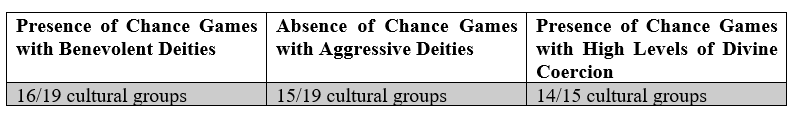
\includegraphics[width=\linewidth]{figures/Davis-Table01}
 		\captionof{table}{Results of Roberts \textit{et al.} (1959) study}
 		\centering
 		\label{fig:Davis-Table01}
 	\end{figure}
 

 
 Comparisons  \IJSRAsection{D-PLACE}between world cultures can provide important insights into human nature and general societal patterns. In the past, comparison was often limited to a small number of case studies within most literature. Now, however, with the advent of D-PLACE \href{http:/www./d-place.org}{www./d-place.org} – an open access database of global cultures, linguistic patterns, and environmental diversity – comparisons between different human groups can be conducted between over 1400 different ‘societies’ \parencite{kirby2016}. A ‘society’ is defined by the D-PLACE database as ``a group of people in a particular locality, who often share a language and cultural identity” \parencite{D-PLACE}. In order to keep terminology as homogeneous as possible, I will refer to such groups as \textit{cultural groups} rather than societies, in order to avoid any confusion in mixing these terminologies.
 
 Utilising D-PLACE, examinations of cultural change, as well as correlations between cultural, linguistic, and environmental variables can be compared between a multitude of different groups \parencite{kirby2016}. By looking at several different variables at once across hundreds (if not thousands) of different cultural groups, many new discoveries can be made that were up until recently, practically impossible. For this study, the Ethnographic Atlas dataset was used, which contains information from over 90 different cultural traits \parencite{kirby2016}. One note on the Ethnographic Atlas data that is necessary to mention is that although it is a global dataset, there is an emphasis on North American and African cultural groups.
 
 When using D-PLACE, searches can be made by a culture group’s name, region(s) of interest, language family, cultural trait(s), or environmental variables. Up to four cultural traits and 3 environmental traits can be compared at one time. Once the desired variables are chosen, data can be visualised in a table, map, or phylogenic tree. Additionally, the data can be downloaded as a .csv file for further use. The most notable trait of D-PLACE is that it gathers a wealth of information and cultural data from a vast collection of literature and data repositories \parencite{kirby2016} that were previously either inaccessible, or extremely difficult to acquire and compare to other sources. This allows for greater scale cross-cultural comparison, and will enable future scholars to conduct studies that address long-time anthropological questions.

\IJSRAsection{Methods}
Using data from D-BASE, several different cultural and geographical comparisons were made addressing some three-hundred different cultural groups from around the world. The first of these comparisons aims at addressing the religious hypothesis of \textcite{roberts1959} and compares 377 different world cultures on the basis of two variables: the presence or absence of games of chance and the presence or absence of High Gods (See \cref{fig:Davis-Table04} in the Appendix).%%Appendix??
 In particular, the presence of ``moralistic” gods or deities that interact with humans was considered for this study. In order to link the presence or absence of ``moralistic” gods to benevolence or aggressiveness as discussed by \textcite{lambert1959} and \textcite{roberts1959}, the following information must be taken into consideration. 

When discussing ``morality” on a supernatural scale, the term refers to the concern a deity – or pantheon of deities – have about human social behaviours \parencite{purzycki2016}. ``Moralizing High Gods” are defined specifically as ``supernatural beings believed to have created or govern all reality, intervene in human affairs, and enforce or support human morality” \parencite[16784]{botero2014}. Furthermore, ``moralistic” gods promote cooperative behaviour while attempting to limit ``antisocial” behaviour \parencite[165]{purzycki2016}. When relating this definition to benevolence or aggressiveness, the following connection can be made: the presence of moralistic gods will contain supernatural beings who are concerned about humanity and will therefore be benevolent towards those who believe in said deity and conform to the values instilled by those gods. Conversely, however, moralistic gods also deliver punishment to those that disobey or fail to act in the manner expected or required by the god(s). As a result, both benevolence and aggressiveness are present within such a classification. On the other hand, in cultural groups without ``moralistic” gods, deities are either unconcerned with human affairs or are extremely distanced from humans, and therefore cannot be considered to be specifically benevolent or aggressive towards humanity. As discussed by \parencite[85]{purzycki2011}, ``[n]ot all supernatural agents, however, are concerned with the general moral behavior of people” and it has been shown using ecological modeling that religious traditions bound to local ecologies emphasise stress on sacrifice, especially in areas that require extensive resource management \parencite{lansing1993}. Cross-cultural analyses have shown that larger and more politically complex human-groups generally have a greater number of moralistic deities \parencite{purzycki2016}. Additionally, in areas that have ``High Gods” that are concerned with human morality, games tend to be more complex \parencite[290]{ball1972}. As a result, assuming the hypothesis of \textcite{roberts1959} is correct, if moralistic gods are present in a cultural group, games of chance should be more abundant. This is the first query of this paper (Q1).

Additional comparisons were conducted to address further correlations between game types, cultural differences, and geographical variables. Comparison was made between 54 cultures on the basis of game type, religious type, and the belief in trance states and possession (see \cref{fig:Davis-Table05} in the Appendix). Assuming that \textcite{roberts1959} is correct in their assumption that games of chance are more abundant in regions that exercise a belief in supernatural intervention, the belief in possession or divine intervention through trance states would be expected to have a statistical relationship with the presence or absence of games of chance (Q2). Comparison between 331 different cultures was also conducted on the basis of game type and mean community population size (see \cref{fig:Davis-Table06a} in the Appendix). Once again returning to \textcite{roberts1959}, assuming that the complexity of a cultural group is said to be correlated with the presence of strategy games and a greater number of different types of games altogether, the larger the population size, the greater the number of games that cultural group should have, including strategy games. Additionally, a look at political integration is explored in relation to the presence of strategy games (see \cref{fig:Davis-Table06b} in the Appendix), following the study of \textcite{roberts1959} (Q3). Finally, the same 377 cultural groups that were compared for Q1 were compared against their geographic positioning (latitude) in order to determine whether or not there is a geographic relationship to game types present in specific populations (Q4).\footnote{The different comparisons, although they contain different numbers of cultural groups, contain many overlaps and many of the cultures compared in one dataset are compared again in later data comparisons.} All of the tables depicting the list of cultures and their traits can be found in the Appendix of this article.

\IJSRAsection{Results; Q1}
Of the 377 cultural groups sampled, 63 had games of chance present. Of these 63 populations, 53 of them also believed in a High God, many of which were ``moralistic” in nature. The other 10 did not believe in a High God that interacted with humans. Conducting a chi-squared test of independence ($n = 377$) revealed a statistically significant result ($\chi^{2} = 32.8, df = 1 p < 0.01$) indicating that a non-arbitrary correlation does exist between the presence of games of chance and the belief in High Gods. Relating the results back to \textcite{roberts1959}, 36 of the 53 cultures that had games of chance believed in a ``moralistic” god that directly intervened into human affairs. Such gods can be considered ``benevolent” – as described by \textcite{lambert1959} – in that they protect humans and instil morals to keep individuals in a state of peace. The other 17 cultural groups did not have ``moralistic” or benevolent gods and did have games of chance present. However, non-moral gods consisted of 128 cultural groups, whereas moralistic gods consisted of 65 cultural groups (see \cref{fig:Davis-Table02}). Statistical analysis of this data revealed that there is a statistically significant correlation between moralistic gods and the presence of games of chance ($n = 193, \chi^{2} = 38.4, df = 1, p < 0.01$).

\begin{figure}[!htb] %TABLE 2
	\includegraphics[width=\linewidth]{figures/Davis-Table02}
	\captionof{table}{}
	\centering
	\label{fig:Davis-Table02}
\end{figure}

\marginnote{Q2}

The second dataset compared trance states, religious type, and game type to test whether or not the belief in supernatural intervention was related to the presence of games of chance. The results disprove this hypothesis, as chi-square testing revealed statistically insignificant results, indicating that any correlation between these variables was likely due to chance ($n = 54, \chi^{2} = 6.77, df = 3, p > .05$).  When looking strictly at possession and excluding trance states, the results were even more independent, as the p-value was close to 0.8, indicating very little relativity between the presence of games of chance and belief in possession. These results do not necessarily mean that the belief in gods that intervene on a person’s behalf have no relevance to the abundance or scarcity of chance games, but statistically, the two variables are unrelated. This indicates that divination practices and the belief in supernatural possession of individuals or objects does not have any significant relationship with the presence of games of chance. However, as will be mentioned later, this does not mean that such beliefs are completely unrelated, as the belief in supernatural intervention in an indirect manner (e.g. fate, karma, etc.) is noticeable as a possible linkage with games of chance.

\marginnote{Q3}

331 different cultures were compared on the basis of game types present and their mean community population size (see \cref{fig:Davis-Table03} in the Appendix).\footnote{It will be noticed that not all culture groups have games. This is not to say that there was no recreational activity or game play of any kind, but rather speaks to the definition of games employed by the researchers and what activities were observed by ethnographers. D-PLACE adheres to the definition of games provided by \textcite{roberts1959} which specifies that ``games” must have an outcome with a winner and loser. As a result, if activities practiced by certain groups did not adhere to this criterion, then the activity would be regarded as recreational, but not a ``game.” Furthermore, if the ethnographers and anthropologists studying certain groups were uninterested in gameplay, then such information would be left out of their research. The way in which the term ``game” has been described by various researchers breeds ambiguity, and therefore, inconsistency within anthropology’s metalanguage is also partly responsible for a lack of data in some regions. This is one of the fundamental reasons as to why concise terminology is required for proper anthropological studies.} When visualising the data (see \cref{fig:Figure1_Davis_082016} and \cref{fig:Figure2_Davis_082016}) a correlation between game types and population size appears, with areas possessing more game types having larger population sizes. This pattern has been noticed by other researchers \parencites{ball1972}[322]{chick1984}[195]{chick1998}{roberts1959}. Overall, areas with larger mean community population sizes tend to have multiple game types present.

\begin{figure}[!htb] %FIGURE 1
	\centering
	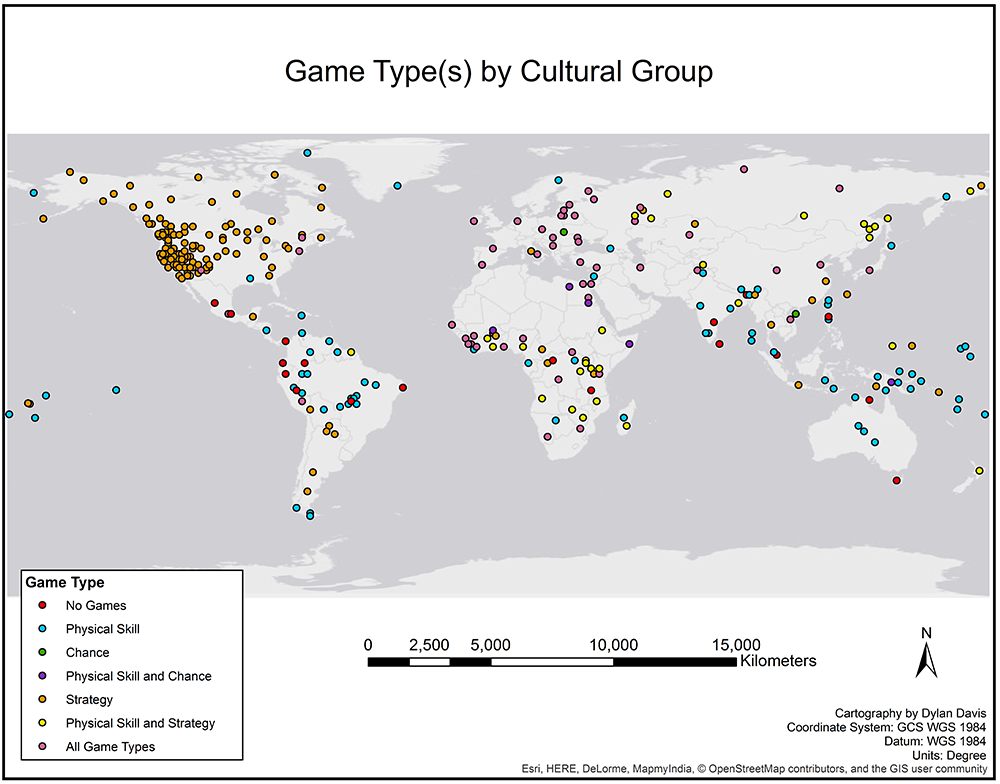
\includegraphics[width=\linewidth]{Davis_Figure1_082016}
	\caption{Map shows the geographic distribution of different game types by cultural group.
	{\normalfont\scriptsize \\ Data Source: \href{http:/www./d-place.org}{www./d-place.org} \copyright\ by 
                 \shortauthor
                 % or NAME OF COPYRIGHT HOLDER
                  }}
	\label{fig:Figure1_Davis_082016}
\end{figure}

\begin{figure}[!htb] %FIGURE 2
	\centering
	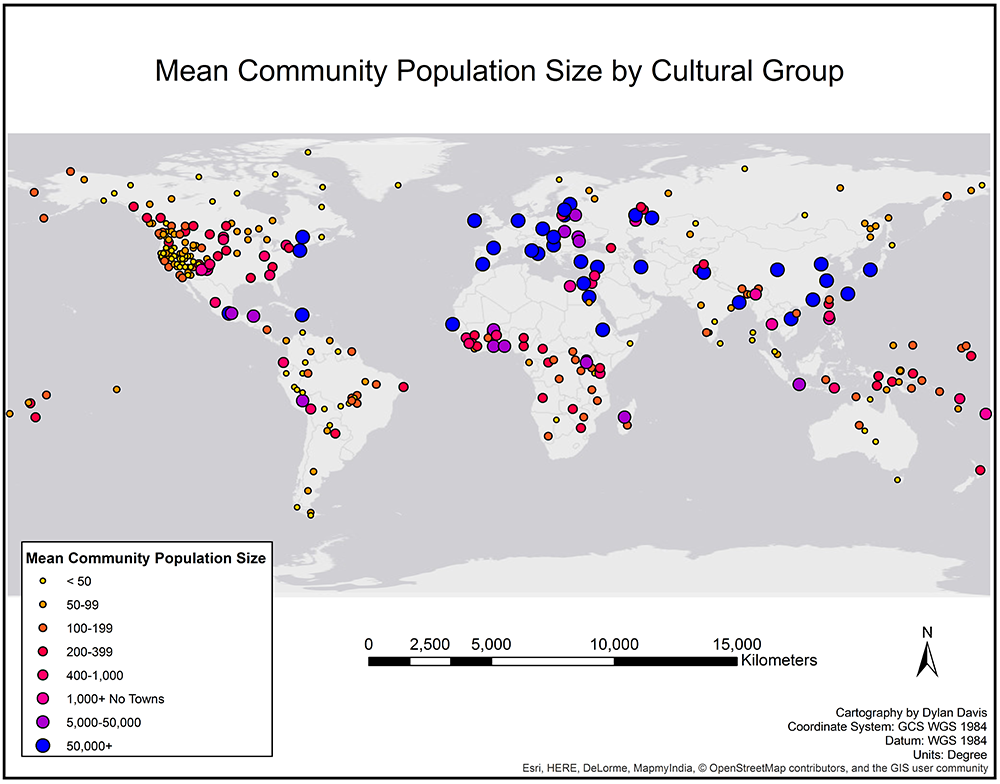
\includegraphics[width=\linewidth]{Davis_Figure2_082016}
	\caption{Map shows geographic distribution of societies based on their average community population size. Areas with larger community sizes tend to be more societally and politically complex.
	{\normalfont\scriptsize \\ Data Source: \href{http:/www./d-place.org}{www./d-place.org} \copyright\ by 
                 \shortauthor
                 % or NAME OF COPYRIGHT HOLDER
                  }}
	\label{fig:Figure2_Davis_082016}
\end{figure}

In addition to comparing game types to mean community population size, a re-visitation of the study conducted by  \textcite{roberts1959} required a direct comparison of game types present in a cultural group to its level of political integration (see \cref{fig:Figure3_Davis_082016}).  \textcite{roberts1959} find that games of strategy are related to greater levels of hierarchical complexity and political integration. In their study, however, only 63 different cultural groups were compared. Utilising D-PLACE, 183 different cultural groups were compared on the basis of political complexity and whether or not games of strategy were present or absent.

\begin{figure} [!htb] %FIGURE 3
	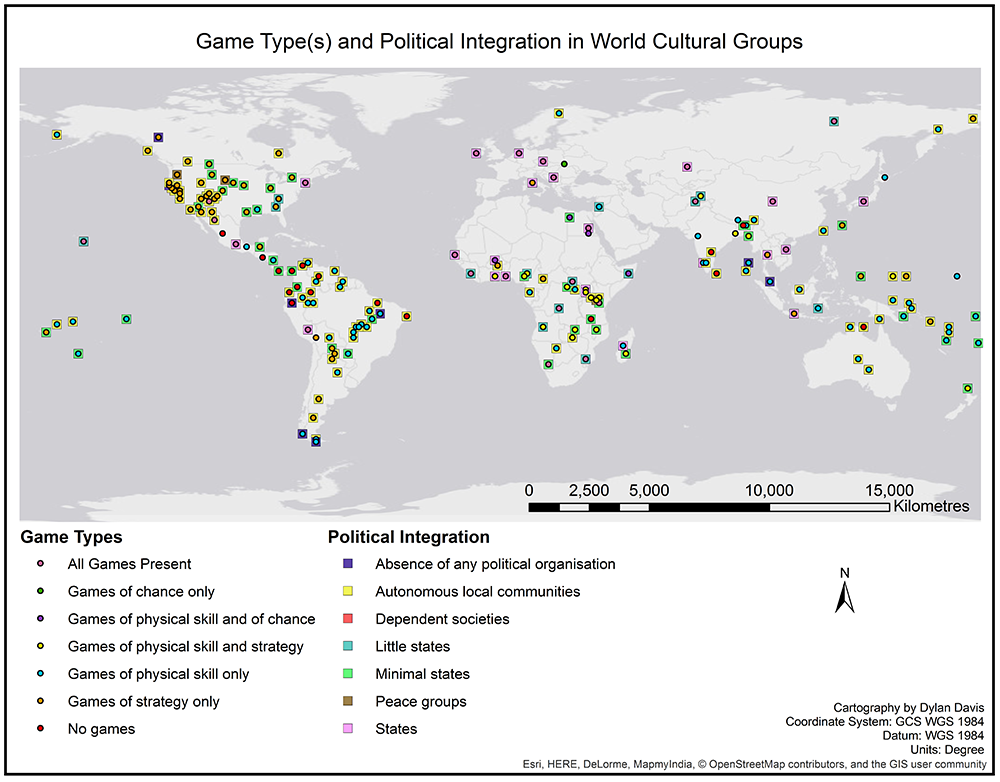
\includegraphics[width=\linewidth]{Davis_Figure3_082016}
	\caption{Map shows game types present and the corresponding level of political integration by cultural group. One pattern that is noticeable is that in State, Minimal State, and Little State societies, most game types are present.
	{\normalfont\scriptsize \\ Data Source: \href{http:/www./d-place.org}{www./d-place.org} \copyright\ by 
                 \shortauthor
                 % or NAME OF COPYRIGHT HOLDER
                  }}
	\label{fig:Figure3_Davis_082016}
\end{figure}

Keeping with \textcite{roberts1959}, complex political organisation was determined on the basis of classifications established by \textcite{murdock1957}. As such the ratings of ``Autonomous Local Communities” and ``No Political Integration” as defined by \textcite{murdock1957} were considered to have ``low political integration” as established by \textcite{roberts1959}, and ``Minimal States”, ``Little States”, and ``States” were considered to have ``high political integration.” Additionally, populations that were classified as ``Absent”, ``Peace Groups”, or ``Dependent” by \textcite{murdock1957} were also considered to have ``low political integration” for this study. The results of a chi-square test of independence shows a high level of statistical significance ($\chi^{2} = 17.8, df = 1, p < 0.01$), indicating that \textcite{roberts1959} is correct in their hypothesis: games of strategy do have a statistical relationship with the level of political integration in a given cultural group.

\marginnote{Q4}
The last query of this paper examines if there are any geographic differences that relate to different game types that are present or absent in various cultural groups. The results are quite interesting. According to a cross-cultural analysis of the same 377 cultural groups examined for Q1, there is indeed a difference between latitudes and game types present, specifically games of chance (see \cref{fig:Davis-Table03} and \cref{fig:Figure4_Davis_082016}). As seen in the map and the table below, the overwhelming majority of cultural groups with games of chance present exist in the northern hemisphere, with 57 out of 63 (\SI{90.5}{\percent}) possessing games of chance existing in the northern hemisphere and only 6 out of 63 (\SI{9.5}{\percent}) existing in the southern hemisphere. Chi square tests reveal these results to be statistically significant ($\chi^{2} = 9.1, df = 1, p < 0.01$). These results were then compared to population sizes and religious types present and show relationships between these variables and geographical location. These results will be discussed in detail in the next section of this paper.

\begin{figure}[!htb] %TABLE 3
	\includegraphics[width=\linewidth]{Davis-Table02}
	\captionof{table}{}
	\label{fig:Davis-Table03}
\end{figure}

\begin{figure}[!htb] %FIGURE 4
	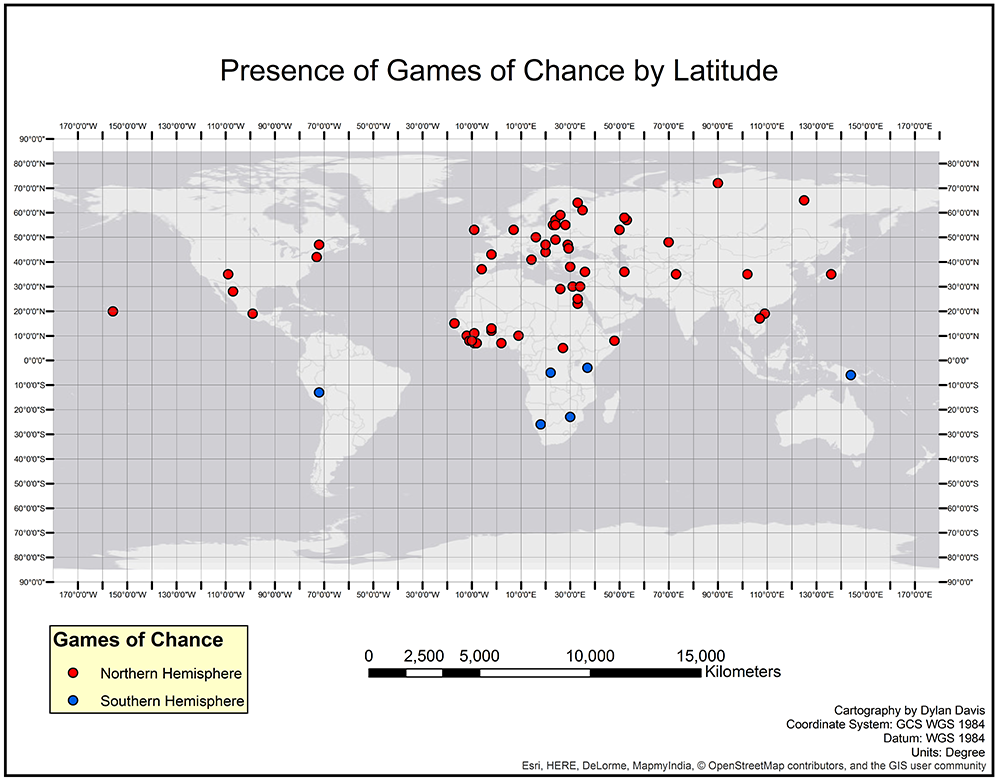
\includegraphics[width=\linewidth]{Davis_Figure4_082016}
	\caption{Map shows cultural groups where games of chance have been discovered. These societies are differentiated based on their latitude. Note, there is no North arrow, only a gradicule showing longitudinal and latitudinal position.
	{\normalfont\scriptsize \\ Data Source: \href{http:/www./d-place.org}{www./d-place.org} \copyright\ by 
                 \shortauthor
                 % or NAME OF COPYRIGHT HOLDER
                  }}
	\label{fig:Figure4_Davis_082016}
\end{figure}
This \IJSRAsection{Discussion}study has four separate enquiries (Q1-Q4), three of which (Q1-Q3) test (either directly or indirectly) different hypotheses proposed by \textcite{roberts1959}. In particular, it is the goal of this study to retest Roberts and colleagues hypothesis that games of chance are related to religious systems, which was unable to be directly confirmed by later studies \parencites[e.g.][]{ball1972}{chick1998}. In fact, little attempt has actually been made to replicate this particular hypothesis of Roberts and colleagues \parencite[18]{binde2005}. Part of the reason for this lack of re-visitation is the low reliability of the data used by \textcite{roberts1959} and the very small sample size \parencite[18]{binde2005}. Despite these limitations, I address the hypothesis utilising a sample size of 377 cultural groups, and test the hypothesis on the basis of the presence of ``moralistic High Gods”, which is similar to a test conducted by \textcite{ball1972}. 

I determine that games of chance are correlated with the presence of ``High Gods” that are ``moralistic” – meaning that the gods are active and supportive of human morality and are involved in the everyday lives of human beings (Q1). This statistical relationship is statistically significant, meaning that the correlation found by \textcite{ball1972}, as well as the results of the study by \textcite{roberts1959}\footnote{\textcite{roberts1959} use a different set of variables for their study. They compare the prevalence of benevolent, aggressive, and coercive gods and their relation to the presence of games of chance. This study tries to bridge the gap between Roberts et al.’s variables and the presence of ``moralistic” gods, asserting that moralistic gods are benevolent to those that follow moral guidelines and are aggressive towards those that do not follow moral guidelines. As a result, in the presence of ``moralistic” gods, benevolence should be at a higher level than with a lack of such deities.}  appear to be more than mere coincidence. This means that the presence of games of chance is linked to the presence of moralistic gods, which can be considered to be ``benevolent” (as hypothesised by Roberts and colleagues). For further illustration, I conducted a kernel density test on the data, which shows overlap between areas with the presence of ``High Gods” and games of chance (see \cref{fig:Figure5_Davis_082016}). On this note, it can also be stated that in many cultures, games of chance, especially gambling, have been associated with spiritual/supernatural power \parencites[22]{binde2005}[147]{binde2007}.

\begin{figure}[!htb] %FIGURE 5
	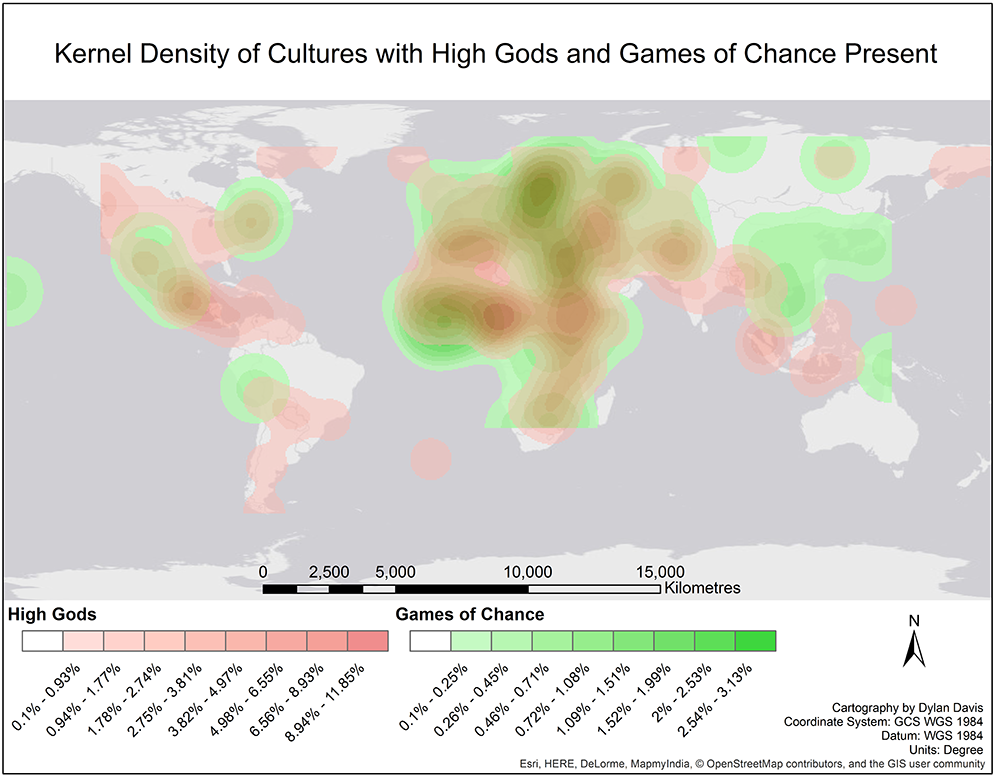
\includegraphics[width=\linewidth]{Davis_Figure5_082016}
	\caption{Map shows densities of societies with High Gods that intervene in human affairs and societies that possess games of chance. It is noticeable that many areas with high densities of one variable have high densities in the other variable as well.
	{\normalfont\scriptsize \\ Data Source: \href{http:/www./d-place.org}{www./d-place.org} \copyright\ by 
                 \shortauthor
                 % or NAME OF COPYRIGHT HOLDER
                  }}
	\label{fig:Figure5_Davis_082016}
\end{figure}

One of the primary reasons for a correlation between religion and games of chance is the concept of illusory control \parencites[see][]{wohl2002}{langer1975}. As stated by \textcite[312]{langer1975}: 
%%%EMBEDDED QUOTE
\begin{quote}
The belief that everyone gets what he deserves denies the operation of chance. It eliminates the necessity for concern and worry over the possibility that aversive events may occur by chance at any time. Events become predictable and thus, by being anticipated, are often controllable.
\end{quote}
%%%EMBEDDED QUOTE
\textcite[323]{langer1975} goes on to state that ``The greatest satisfaction or feeling of competence” will ``result from being able to control the seemingly uncontrollable.” According to the concept of illusory control, individuals desire control over most (if not all) aspects of life, and will thus find some way in which to gain control over a situation. The possession of power has been found to lead to illusory control – or a state of perceived control over the outcome of certain situations \parencite{fast2009}. As a result, those that believe in supernatural powers will be more likely to develop correlations between chance and divine intervention, thereby developing a sense of illusory control in such situations in order to control the outcomes of such games \parencite[1089]{tobacyk1991}.

Looking at the results of Q2, I find that there is no statistically significant relationship between trance states and possession and the presence of games of chance. What this means is that although the presence of gods that intervene in human affairs is correlated with games of chance, the intervention on behalf of the supernatural to influence the outcome of a game is not statistically relevant to the presence of chance games. This result suggests that the presence of a ``moralistic” god instils a set of morals indicating right and wrong, and thereby offers guidelines for what constitutes individuals who are ‘good’ and those that are ‘bad’. Furthermore, for individuals who are deemed ‘bad’ by their god(s), it is suggested that punishment will befall them, and benefits will come to those who are deemed ‘good’. Therefore, although direct intervention is unrelated to the presence of games of chance, the belief in some type of karma or consequence for one’s actions can be said to be related to the presence of chance games. On this point, \textcite{robinson2015} asserts that:
%%%EMBEDDED QUOTE
\begin{quote}
The common game of Snakes and Ladders originated in India and the early boards were adorned with Hindu gods. The random elements of the game had their roots in Karma and the player's fortune was seen as being determined not as a random act but by fate. In Ancient Egypt these random elements may have been seen as the destiny of the gods also, as being governed by the universal truth of Maat.
\end{quote}
%%%EMBEDDED QUOTE
Thus, games of chance – like the game of Snakes and Ladders – in India and Egypt were rooted in beliefs in fate and divine intervention, thereby highlighting the interconnectivity between religious beliefs and the popularity of games of chance.

It must be understood that a connection between material culture and religion is not unexpected. Religion is but a set of ideals, whereas ritual constructs a tangible relationship between those ideals and extant social systems \parencite[14]{bell1992}. As such, material entities are a crux to the existence and success of a religious system. Material objects allow people to ``participate in the divine and to use religion as a technology to manage the beyond of the world in which we live” \parencite[99]{hodder2016}. Games are one such means to an end. 

Relating the results of Q1 and Q2 to \textcite{roberts1959}, it can be affirmed that the belief in gods who are benevolent (i.e. moralistic and deal reward as well as punishment) is statistically related to the presence of games of chance. However, direct aid by the supernatural – which is used by \textcite[602]{roberts1959} as a justification for their results – cannot be said to be true. Nonetheless, religion and games of chance do appear to be correlated, thus reaffirming the results of Roberts and colleagues.

Additional evidence in support of these conclusions comes from the archaeological site of Vijayanagara in southern India. Within this city were many palaces, temples, and shrines, and in association with these features many game-boards were discovered, engraved within stone on or near these architectural structures \parencite[462-463]{rogersdotter2015}. \textcite{rogersdotter2015} classifies the different game-boards found at Vijayanagara into six different categories: alignment games, hunt games, war games, race games, mancala games, and unspecified game types. Of these classes, race games were based on chance, relying on the rolling of dice or throwing of sticks. Consequently, \textcite{rogersdotter2015} finds that race games were the most abundant game type found within the site of Vijayanagara. Additionally, as a major city with a large and socio-economically diverse population, Vijayanagara possessed a large number of the six different types of game boards, consisting of games of chance and strategy. 

In Ancient Egypt particularly (but many other areas as well), the games of \textit{senet} and \textit{mehen} were often played in social contexts, particularly during funerals \parencite[34]{kendall2007}. Both \textit{senet} and \textit{mehen} are considered ``race games”, whereby the objective is to reach a certain point on the game-board and usually includes some type of randomizing agent such as dice \parencite[3]{gobet2004}. In \textit{senet}, casting sticks and \textit{astragali} (knucklebones) were often used (rather than dice) and the game itself became entangled with funerary rites and religious ritual \parencites{piccione1980}[58]{piccione2007}. \textit{Senet} came to be viewed as an activity that bridged the gap between the dead and the living, whereby the game itself acted as a method of communication between the two worlds \parencites[59]{piccione2007}{robinson2015}. Additionally, \textit{mehen} was often found in similar contexts to \textit{senet}, and was also linked with the afterlife \parencite[40-41]{kendall2007}. Both of these games have been found with the context of tombs, signaling their connection to death and journey to the afterlife. Another game similar to \textit{mehen}, called the ``Hyena Game” appeared after \textit{mehen} lost popularity and too comprised a multitude of cosmological motifs \parencite[44]{kendall2007}. Both \textit{mehen} and the ``Hyena Game” contain the same ritualistic meaning, as described by \textcite[44]{kendall2007}: ``the first player to exit the board may well have been thought actually to become \textit{Mehen}, so that the small lion [game] pieces may have been conceptualized as the instruments by which the snake [the board was constructed in the shape of a snake] could destroy the ‘enemies of \textit{Re}’.” As such, games such as \textit{senet}, \textit{mehen}, and offshoots such as the ``Hyena Game” are metaphysical constructs between the realms of the living and the dead, and as such are often recovered in funerary contexts (i.e. tombs). These games are chance based, and therefore illustrate how religious beliefs can affect the types of games played, and the contexts in which those games are played. 

One final example illustrating the connection between religion and games of chance comes from the Zuni culture. Zuni (or Zu\~{n}i) is a Native American group located in the Southwest of the United States. The Zuni possessed all three major game types – strategy, physical skill, and chance (see Appendix \cref{fig:Davis-Table06a} and \cref{fig:Davis-Table06b}). Games like \textit{sh\'{o}liwe} (a gambling game involving arrow reeds) were said to have originated with the Zuni Gods of War, and was then passed to the Zuni people by their mythical ancestors \parencite[480]{stevenson1903}. The game itself is played ceremonially to induce rain, but can also be played outside of this realm as a normal gambling activity \parencite[480]{stevenson1903}. Thus, \textit{sh\'{o}liwe} is rooted in religious beliefs, but also contains a secular nature. Additionally from \textit{sh\'{o}liwe}, other games revolving around chance also existed, some of which were also linked to mythology and religion \parencite{stevenson1903}. 

The next enquiry (Q3) was devoted to looking at political complexity and their relations to the presence of different game types. The results of a cross-cultural comparison of 331 different cultural groups reveal a correlation between population size and the number of different game types present. This result was not unexpected, due to the repeated conclusion that political complexity is related to a more complex series of games and a larger number of game types \parencites[291]{ball1972}[322]{chick1984}[195]{chick1998}{chick2015}{peregrine2008}{roberts1959}. In addition to this test, comparison between political integration level was compared to the presence of strategy games in order to retest another hypothesis established by \textcite{roberts1959} and retested by \textcite{chick1998}, but this time with a larger sample size ($n = 183$). The results once again reaffirm that games of strategy are related to higher levels of political integration.\footnote{This is also supported by evidence from Vijayanagara \parencite{rogersdotter2015}}.

The last area of investigation in this paper is separate from the \textcite{roberts1959} study, and looks at geographical differences for the distribution of game types (Q4). The results indicate that games of chance are overwhelmingly abundant in the northern hemisphere. This result was then compared to mean community population sizes and the presence or absence of ``moralistic” gods. What was determined is that in almost all of the cultural groups included in the sample ($n = 377$) that had games of chance ($n = 63$), \SI{90.5}{\percent} (57 out of 63) of them have either moralistic gods or gods that intervene in human affairs (see \cref{fig:Figure6_Davis_082016}). Additionally, in the areas that had such deities present, most had mean community population sizes of at least \num{50000} persons (see \cref{fig:Figure7_Davis_082016}). 
Conclusions that can be drawn from these spatial patterns are that chance and religion are correlated, and religion and population size are correlated. Therefore, religion and population size are correlated, and the presence of games of chance (like all game types) is related to the population level present in a group. 
The fact that the majority of cultures possessing ``moralistic” gods and games of chance are located in the northern hemisphere is linked to the fact that the vast majority of large population centres are located in the northern hemisphere.

There are a number of variables which influence where people establish themselves and how they develop. Especially important in regards to the establishment of different cultural groups are environmental variables. In a study conducted by \textcite{botero2014}, it is determined that populations possessing a belief in moralising high gods are more prevalent in areas that are at exposed to greater levels of ecological pressure. \textcite[16786]{botero2014} examine 583 cultural groups and determine that the belief in moralistic high gods is directly correlated to political complexity, spatial proximity to other cultures that believe in such deities, ecological variables, the presence of animal husbandry and agriculture, and linguistic origins. This sheds some light on why the distribution of religious systems is uneven: they are linked to a plethora of other factors, including the environment.\footnote{For a detailed discussion of the relationship between religion and environmental factors, \textcite{davis}. In particular, Davis argues that religious systems can reinforce environmentally conscious practices, and such religious ideologies can influence innovation and the use of resources.} Furthermore, due to the fact that game types are related to the religious beliefs present, they too are related to population size, political complexity, technology, and ecological factors present in an area. Therefore, environmental differences may have some effect on the game types present in a given cultural group. One should be critical of generalisations however, and further studies should be undertaken to confirm or dismiss such a claim.

\begin{figure}[!htb] %FIGURE 6
	\includegraphics[width=\linewidth]{Davis_Figure6_082016}
	\caption{Map shows the geographic distribution of different religious types (i.e. presence of "moralistic" gods) and the presence of games of chance.
	{\normalfont\scriptsize \\ Data Source: \href{http:/www./d-place.org}{www./d-place.org} \copyright\ by 
                 \shortauthor
                 % or NAME OF COPYRIGHT HOLDER
                  }}
	\label{fig:Figure6_Davis_082016}
\end{figure}

\begin{figure}[!htb] %FIGURE 7
	\includegraphics[width=\linewidth]{Davis_Figure7_082016}
	\caption{Map shows the geographic distribution of religious types (i.e. presence of High Gods) and average community population sizes for various world cultures. Note, a graticule is used in lieu of a North Arrow to show latitudinal and longitudinal location.
	{\normalfont\scriptsize \\ Data Source: \href{http:/www./d-place.org}{www./d-place.org} \copyright\ by 
                 \shortauthor
                 % or NAME OF COPYRIGHT HOLDER
                  }}
	\label{fig:Figure7_Davis_082016}
\end{figure}

\IJSRAsection{Conclusion}

Cross-cultural comparisons have long been undertaken, and have oftentimes been severely limited in their sample sizes due to an inability to access data, or a lack of data altogether. Using a new database of cultural variables \parencite{D-PLACE} a re-visitation of one of the most influential cross-cultural analyses of gaming \parencite{roberts1959} is carried out to retest the almost 60 year old hypotheses. In particular, attention is placed on Roberts and colleagues’ hypothesis about games of chance and religion. The results of this study indicate that the presence of games of chance is correlated with the presence of benevolent ``moralistic” gods, therefore reaffirming Roberts and colleagues’ hypothesis. However, the presence of a belief in supernatural intervention (i.e. possession of people or objects) shows no relation to the presence or absence of chance games. The belief in divine intervention was used by \textcite[601--602]{roberts1959} as a justification for a linkage between religion and chance games, but has been invalidated by this study. Additionally, other aspects of the \textcite{roberts1959} study are reinvestigated, particularly the relation between game types and socio-political complexity. All components of the Roberts et al. study – minus a link between divine intervention and chance games – appear to be valid.

For archaeologists, these conclusions reaffirm that games, especially games of chance, possess ritual importance and can be linked to ritualistic activities. Additionally, the presence of games in an archaeological site can suggest about the area’s population size, religious system, and political integration level. The use of online databases (like D-PLACE) also has important benefits to archaeologists, who can now compare certain elements of archaeological cultures with other cultural groups in the same geographic region, or across the globe, allowing for a global comparison of the archaeological record. Such studies can enlighten us about human nature, cultural diffusion patterns, and the diversity of humans, as well as their similarities, throughout the globe.

Separate from retesting old conclusions, a cross-cultural investigation into the presence of certain types of games in relation to latitude was conducted, revealing that the northern hemisphere has more variety, and a greater number of cultural groups that possess games of chance, as well as religious systems with ``moralistic” gods. The reasoning for this spatial patterning is left to be explored, but should be the focus of future anthropological research. Correlations between gods, games, and geography exist across cultures, and can give important insights for archaeologists, anthropologists, and social scientists in general.



\IJSRAclosing%<---- don’t change this!
\end{document}


%------------------------------
\part[Literature Reviews]{\scshape literature reviews}\thispagestyle{empty}
%\documentclass[%
	%draft
%	]{ijsra}
\def\IJSRAidentifier{\currfilebase} %<---- don’t change this!
%-------Title | Email | Keywords | Abstract-------------
\def\maintitle{A Reassessment of Natufian Sedentism}
\def\shorttitle{\maintitle}
\def\cmail{sgyn3538@uni.sydney.edu.au}
\def\keywords{Near Eastern Archaeology, Natufian, Settlement Dynamics, Mobility and Sedentism}

%\def\keywordname{}%<--- redefine the name “Keywords“ in needed language
\def\abstract{The Natufian assemblage (ca. \num{13000}–\num{10300} years BP) in the Levant has largely been understood to reflect sedentary communities. However, thorough analysis of the material has demonstrated that a misunderstanding of sedentism and misinterpretations of cultural material have driven this claim. Scholars including Edwards and Shewan have significantly contributed to the debate and convincingly argued for Natufian mobility. This literature review summarises early thought and study of Natufian sites and identifies the strengths and weaknesses. It then discusses more recent research and opinions that challenge long held notions of Natufian sedentism. The Natufian assemblage represents a key period in the history of human behaviour, and consequently, a comprehensive and rigorous analysis of the Natufian assemblage is important for understanding the transition from mobile to sedentary communities, and the material culture that results. A review and consideration of the various aspects of the debate is necessary for continuing further research.}
%--------Author’s names------------
\def\authorone{Sarah Gyngell}
%-------Biographical information-------------
\def\bioone{Sarah is an undergraduate student at the University of Sydney where she is completing a Bachelor of Arts and Science majoring in Archaeology and Marine Science. She plans to study Epipaleolithic Near Eastern Archaeology for her Honours, with a focus on changing settlement dynamics during the mobile to sedentary transition. Sarah hopes to apply her background in geoscience and the use of GIS to contribute to future research. She has field experience in Jordan, where she was a volunteer at Pella in 2015. Sarah has also worked at a historic site in Sydney and volunteered for numerous organisations and events including the 2015 Australian National Archaeology Student Conference.}
%------University/Institution--------------
\def\affilone{Department of Archaeology, University of Sydney}

\begin{filecontents}{\IJSRAidentifier.bib}
%Bibliography-data HERE
@incollection{Bar-Yosef_1983,
	author = {Bar-Yosef, O.},
	editor = {Young, T. and Smith, P. and Mortensen, P.},
	title = {The Natufian in the Southern Levant},
	booktitle = {The Hilly Flanks and Beyond: Essays on the Prehistory of 	Southwestern Asia},
	date = {1983},
	pages = {11--42},
	publisher = {The Oriental Institute of the University of Chicago},
	location = {Chicago},
}

@article{Bar-Yosef_1998,
	author = {Bar-Yosef, O.},
	title = {The Natufian Culture in the Levant, Threshold to the Origins of 	Agriculture},
	journaltitle = {Evolutionary Anthropology},
	date = {1998},
	pages = {159-–177},
	volume = {6},
}

@article{Bar-Yosef_2011,
	author = {Bar-Yosef, O.},
	title = {Climatic Fluctuations and Early Farming in West and East Asia},
	journaltitle = {Current Anthropology},
	date = {2011},
	pages = {S175--S193},
	volume = {52},
	series= {4},
}



@incollection{Fletcher_1998,
author = {Fletcher, R.},
title = {African Urbanism},
subtitle = {Scale, Mobility and Tranformations},
editor = {Connah, G.},
booktitle = {Transformations in Africa},
pages = {104-138},
year = {1998},
location = {London},
publisher = {Leicester University Press},
}


@article{Bar-Yosef_1989,
	author = {Bar-Yosef, O. and Belfer-Cohen, A.},
	title = {The Origins of Sedentism and Farming Communities in the Levant},
	journaltitle = {Journal of World Prehistory},
	date = {1989},
	pages = {447--498},
	volume = {3},
	issue = {4},
}

@incollection{Bar-Yosef_1991,
	author = {Bar-Yosef, O. and Valla, R.},
	editor = {Bar-Yosef, O. and Valla, R.},
	title = {The Natufian Culture: An Introduction},
	booktitle = {The Natufian Culture in the Levant},
	date = {1991},
	pages = {1--10},
	publisher = {International 	Monographs in Prehistory},
	location = {Michigan},
}

@article{Belfer-Cohen_1991,
	author = {Belfer-Cohen, A.},
	title = {The Natufian in the Levant},
	journaltitle = {Annual Review of Anthropology},
	date = {1991},
	volume = {20},
	pages = {167--186},
}

@incollection{Belfer-Cohen_2013,
	author = {Belfer-Cohen, A. and Goring-Morris, A.},
	editor = {Bar-Yosef, O. and Valla, F.},
	title = {Breaking the Mould: Phases and Facies in the 	Natufian of the Mediterranean Zone},
	booktitle = {Natufian 	Foragers in the Levant: Terminal Pleistocene Social Changes in Western Asia},
	date = {2013},
	pages = {544--561},
	publisher = {International 	Monographs in Prehistory},
	location = {Michigan},
}

@book{Byrd_2005,
	author = {Byrd, B.},
	title = {Early Village Life at Beidha, Jordan: Neolithic Spatial Organisation and Vernacular Architecture},
	date = {2005},
	publisher = {Oxford University Press},
	location = {New York},
}

@article{Boyd_2006,
	author = {Boyd, B.},
	title = {On ‘sedentism’ in the Later Epipalaeolithic (Natufian) Levant},
	journaltitle = {World Archaeology},
	date = {2006},
	volume = {38},
	issue = {2},
	pages = {164--178},
}

@book{Childe_1953,
	author = {Childe, V.},
	title = {New Light on the Most Ancient Near East},
	date = {1953},
	publisher = {Praeger},
	location = {New York},
}

@article{Edwards_1989,
	author = {Edwards, P. C.},
	title = {Problems of recognising earliest sedentism: the Natufian example},
	journaltitle = {Journal of Mediterranean Archaeology},
	date = {1989},
	volume = {2},
	pages = {5--48},
}

@book{Edwards_2013,
	author = {Edwards, P. C.},
	title = {Wadi Hammeh 27, an Early Natufian Settlement at Pella in Jordan},
	date = {2013},
	publisher = {Brill},
	location = {Leiden},
}

@article{Edwards_2015,
	author = {Edwards, P. C.},
	title = {Natufian interactions along the Jordan Valley},
	journaltitle = {Palestine Exploration Quarterly},
	date = {2015},
	volume = {4},
	issue = {147},
	pages = {272--282},
}

@article{Finlayson_2013,
	author = {Finlayson, B.},
	title = {Imposing the Neolithic on the past},
	journaltitle = {Levant},
	date = {2013},
	volume = {45},
	issue = {2},
	pages = {133--148},
}


@book{Fletcher_2007,
	author = {Fletcher, R.},
	title = {The Limits of Settlement Growth: A Theoretical Outline},
	date = {2007},
	publisher = {Cambridge University Press},
	location = {Cambridge},
}

@article{Garrod_1957,
	author = {Garrod, D.},
	title = {The Natufian culture: the life and economy of a Mesolithic people in the Near East},
	journaltitle = {Proceedings of the British Academy},
	date = {1957},
	issue = {43},
	pages = {211--227},
}

@article{Habu_1996,
	author = {Habu, J.},
	title = {Jomon sedentism and intersite variability: collectors of the Early Jomon Moroiso Phase in Japan},
	journaltitle = {Arctic Anthropology},
	date = {1996},
	volume = {33},
	issue = {2},
	pages = {38--49},
}

@article{Hardy-Smith_2004,
	author = {Hardy-Smith, T. and Edwards, P. C.},
	title = {The garbage crisis in prehistory: artefact discard patterns at the Early Natufian site of Wadi Hammeh 27 and the origins of household refuse disposal strategies},
	journaltitle = {Journal of Anthropological Archaeology},
	date = {2004},
	issue = {23},
	pages = {253–-289},
}

@incollection{Lieberman_1999,
	author = {Lieberman, D.},
	editor = {Rocek, T. and Bar-Yosef, O.},
	title = {Natufian “Sedentism” and the Importance of Biological Data for 	Estimating Reduced Mobility},
	booktitle = {Seasonality and Sedentism: Archaeological Perspectives from Old and New World Sites},
	date = {1999},
	publisher = {Peabody Museum of Archaeology and Ethnology},
	location = {Harvard University},
	pages = {75--92},
}

@book{Parslow_2009,
	author = {Parslow, C.},
	title = {Social Interaction in the Prehistoric Natufian: Generating an interactive agency model using GIS},
	date = {2009},
	publisher = {Archaeopress},
	location = {Oxford},	
}

@incollection{Shewan_2004,
	author = {Shewan, L.},
	editor = {Delage, C.},
	title = {Natufian Settlement Systems and Adaptive Strategies: The Issue of Sedentism and the Potential of Strontium Isotope Analysis},
	booktitle = {The Last Hunter-Gatherer Societies in the Near East},
	date = {2004},
	publisher = {John and Erica Hedges},
	location = {Oxford},
	pages = {55--94},
}

@article{Stutz_2002,
	author = {Stutz, A.},
	title = {Polarizing microscopy identification of chemical diagenesis in 	archaeological cementum},
	date = {2002},
	journaltitle = {Journal of Archaeological Science},
	issue = {29},
	year = {2002},
	pages = {1327–-1347},
}

@incollection{Tchernov_1991,
	author = {Tchernov, E.},
	editor = {Bar-Yosef, O. and Valla, F.},
	title = {Biological evidence for human sedentism in southwest Asia during 	the Natufian},
	booktitle = {The Natufian Culture in the Levant},
	date = {1991},
	pages = {315–-340},
	publisher = {International 	Monographs in Prehistory},
	location = {Michigan},
}

@incollection{Valla_1999,
	author = {Valla, F.},
	editor = {Rocek, T. and Bar-Yosef, O.},
	title = {Natufian Seasonality: A Guess},
	booktitle = {Seasonality and Sedentism: Archaeological Perspectives from Old and New World Sites},
	date = {1999},
	publisher = {Peabody Museum of Archaeology and Ethnology},
	location = {Harvard University},
	pages = {93--108},
}

@article{Yeshurun_2014,
	author = {Yeshurun, R. and Bar-Oz, G. and Weinstein-Evron, M.},
	title = {Intensification and sedentism in 	the terminal Pleistocene Natufian sequence of el-Wad Terrace (Israel)},
	journaltitle = {Journal of 	Human Evolution},
	date = {2014},
	issue = {70},
	pages = {16--35},
}


\end{filecontents}
%\begin{document}
\IJSRAopening%<---- don’t change this!
%-------

%\IJSRAsection{Introduction}
\lettrine{T}{he} Natufian assemblage in the Levant is significant for human behaviour due to its relevance to issues concerning the transition from mobile to sedentary communities. Thus, it has attracted considerable attention and research has produced a diversity of interpretations and arguments. 
The Natufian sites and assemblages discovered in the 1930s were initially interpreted as representative of a sedentary lifestyle due to the appearance of stone architecture and evidence of agriculture. These cultural markers were key to the \textcite{Childe_1953} prominent model of the Neolithic revolution, and the belief that agriculture and sedentism were exclusively linked heavily influenced this understanding. In recent decades several archaeologists, to be discussed here, have demonstrated errors in these assumptions and have convincingly argued that mobile communities are capable of farming and building stone structures, hence disputing the primary premise for claiming Natufian sedentism. However, preference for Natufian sedentism remains pervasive in modern debate and a thorough analysis of the literature is important to discern the strengths and weaknesses of the arguments of both sides. 

Archaeologists including Bar-Yosef and Valla made significant contributions to the wealth of material concerning the Natufian and strong arguments characterising Natufian material culture. Bar-Yosef made strong links between paleoclimate reconstructions and the appearance of agriculture in the Natufian, and developed detailed models of Natufian site hierarchy. However, Bar-Yosef and other scholars have not reassessed the underlying principles, devised in the early \nth{20} century, guiding their research. In contrast, research by scholars including Edwards and Shewan, demonstrated considerable evidence for Natufian mobility. \textcite{Edwards_1989} verified the incapability of cultural markers to indicate sedentism and instead demonstrated the similarities of Natufian material culture with mobile communities. 
Furthermore, \textcite{Shewan_2004}, using innovative scientific analysis, demonstrated the mobile nature of people in the Natufian landscape. 
Considering the importance of the evident behavioural transformation that occurred in this time period, future research should continue in a direction away from inferences founded on early assumptions and towards rigorous examination of the evidence. The application of the \textcite{Fletcher_2007} outline of prerequisites for sedentism, along with a quantified assessment of changes in settlement structure using GIS, would be an insightful contribution to the debate.

\IJSRAsection{Natufian Discovery} 
Early interpretations of the Natufian were established on preconceived notions and limited evidence, resulting in the identification of Natufian settlements as agricultural villages. \textcite{Garrod_1957} described a distinctive lithic industry and burials in Shukbah Cave to classify the Natufian as a separate cultural complex to the preceding Kebaran. Her initial argument that the Natufian assemblage reflected the earliest farmers resulted in their identification as sedentary, due to the misunderstanding that one must equate with the other. 
\textcite{Garrod_1957} argued that the large number of sickle blades in Natufian sites was evidence of harvesting, and furthermore, believed stone structures reflected long-term settlement and substantial investment. 
Garrod’s interpretation of the Natufian as agriculturalists, determined by evidence of sickle gloss on flint blades, has since been reconsidered \parencite[75]{Lieberman_1999}. 
Instead, it has been proposed that the Natufian represented an increase in cultural complexity that formed a foundation for agriculture in the Neolithic, often attributed to the impact of environmental variability \parencite[447]{Bar-Yosef_1989}. 

However, claims for Natufian sedentism persist decades on. It appears possible that Garrod and other early researchers imposed preconceptions of the Natufian and their understanding of the significance of the period onto their analysis of the data \parencite{Finlayson_2013}.
This resulted in inadequate testing of hypotheses and the development of an inaccurate representation of the Natufian. Furthermore, Garrod failed to provide a comprehensive definition of sedentism and demonstrate how it applied to the Natufian.

\IJSRAsubsection{Bar-Yosef}
Throughout the course of the debate Ofer Bar-Yosef made a significant contribution to the wealth of data to be examined and provided a platform for the Natufian to be discussed. However, he has not moved definitively away from the idea of the Natufian as sedentary. 
In the 1970s and 1980s Bar-Yosef attempted to fit Natufian assemblages into schemes and models of Natufian settlement strategies to reflect organised social systems \parencite[25]{Bar-Yosef_1983}. 
He differentiated sites into base camps and seasonal camps relative to the intensity of the stone tool assemblage and size of structures \parencite[14]{Bar-Yosef_1983}. 
He proposed that a site hierarchy existed and several seasonal camps would be situated within the same territory as a large base camp \parencite[25]{Bar-Yosef_1983}. 
Although he has challenged early assertions that base camps such as Eynan could be considered permanent villages based on architectural evidence, he supported the argument that commensal species reflect sedentary settlements \parencite[5]{Bar-Yosef_1991}. 
Consequently, he defined Hayonim Terrace as a permanent Natufian settlement \parencite[25]{Bar-Yosef_1983}.  
However, he failed to define a length of occupation necessary to classify permanency to support this claim. Although he recognised the deficiency in his argument, he continued to emphasise the differences between Natufian assemblages and preceding cultures to argue that they were sufficient to reflect a transition from mobile to sedentary. 
These include an increase in the amount of investment in stone structures, commensals and overall quantity of cultural material \parencite[6]{Bar-Yosef_1991}. Although there is strong evidence for these differences, he did not demonstrate how they clearly link with claims for sedentism. 
Instead, \textcite[56]{Shewan_2004} argued strongly that they simply reflect a transition to complex mobile communities. 

In more recent decades, Bar-Yosef linked palaeoclimate data with Natufian settlement patterns and subsistence strategies. \textcite[157]{Bar-Yosef_1998} identified the region of the ‘Natufian Homeland’ and argued that the sequence of changes in the area, predominantly the appearance of sedentary Natufian hamlets and the subsequent Neolithic cultivators, should be understood in the context of changing paleobotanical conditions. The application of palaeoenvironmental reconstruction to interpreting archaeological assemblages made a significant contribution to an understanding of the period. 
However, to suggest that the Natufian assemblage can be explained by changes in climate is limiting and implies that due to the suitable environmental conditions for agriculture and year-round settlement occupation \num{12000} years BP, the Natufian should exhibit this behaviour to some extent \parencite[161]{Bar-Yosef_1998}. This argument of environmental determinism is flawed due to examples of advantageous climate where agriculture and sedentism do not occur, demonstrating the need to consider the role of other factors. 
Along with \textcite{Valla_1999}, Bar-Yosef argued that the richness of Natufian assemblages and their success was aided by favourable climatic conditions. 
Although the environment no doubt plays an external role in the development of Natufian subsistence, the argument for a direct cause and effect between the two limits the debate \parencite{Fletcher_2007}. 
Finally, \textcite[175]{Bar-Yosef_2011} continued to discuss how the Natufian relates to the Neolithic and, in doing so, attempted to find evidence for agricultural origins in the Natufian. 
\textcite{Finlayson_2013}.
demonstrated the tendency of Near Eastern archaeologists to impose their understanding of the significance of the Neolithic onto their interpretations. Bar-Yosef and Valla exemplified this by making links between the two assemblages before they were well founded, and discussing the Natufian as a precursor to the Neolithic, rather than how the Natufian assemblage itself developed. 

\IJSRAsubsection{Commensalism and Seasonality}
Several Near Eastern scholars have similarly proposed varying degrees of Natufian sedentism and have developed potential models to describe their settlement strategies, often in relation to climate and the origins of agriculture. A dominant theme in the debate is the issue of commensalism proposed by Tchernov. \textcite[315]{Tchernov_1991} identifies sedentary life in the archaeological record following the appearance of new animal species in a mutualistic relationship with humans. 
He argues permanent settlement is required for commensalism to occur \parencite[316]{Tchernov_1991}. 
Therefore with respect to the Natufian, \textcite[318]{Tchernov_1991} argues that evolutionary changes in bird and rodent populations surrounding Natufian sites, such as Hayonim cave, was a result of long-term human occupation. 
However, the adaptation of animals to develop a relationship with humans has been experimentally demonstrated to require no longer than three months \parencite[173]{Boyd_2006}. Commensalism is a strong argument for demonstrating a change in human settlement behaviour; however, it does not conclusively validate claims for sedentism. 
Instead, it is argued that commensals are present in many non-sedentary contexts, and other factors besides occupation length may lead to their presence in the archaeological record \parencite{Boyd_2006}. This data could be used to indicate seasonally occupied sites, which may help in understanding the transition from mobile to sedentary.

The relationship between seasonality and sedentism has also been of interest to archaeologists. \textcite{Valla_1999} described a system of seasonality that includes an aggregation phase and dispersal phase, dependent on the availability of seasonal resources. 
He argued that equilibrium was reached between these two phases as the length of the aggregation increased with the tendency to return to the same site \parencite[94]{Valla_1999}. 
\textcite{Lieberman_1999} also argued for Natufian sedentism following his study of seasonal hunting data. 
His analysis of cementum bands of gazelle teeth led to his conclusion that Natufian sites were occupied on a multi-seasonal basis \parencite[75]{Lieberman_1999}. 
However, more recent study argues that post-depositional leaching of collagen may effectively mimic seasonal cementum growth layers \parencite{Stutz_2002}. 
Hence, this analysis cannot be considered reliable or an effective indicator of mortality and seasonality \parencite{Stutz_2002}. 
Finally, \textcite[167]{Belfer-Cohen_1991} supported the commonly espoused notion that Natufian settlement is indicative of sedentism due to larger investment and effort in building structures and the occurrence of storage facilities. 

These arguments often include minimal consideration of the evidence for mobility and underestimate the capabilities of mobile groups to build permanent structures. Furthermore, global cross-comparison and a detailed analysis of mobility in African agrarian-based communities has determined that the minimum duration required for sedentism is between five and seven years \parencite[115]{Fletcher_1998}. 
Although these scholars are recognising a change in human settlement patterns, this change cannot be considered to be sedentism. The tendency to assume sedentism continues, despite the evidence for seasonal movement \parencite{Edwards_1989}.

\IJSRAsubsection{Semi-Sedentism}
In recent years several of the above-mentioned scholars became somewhat tentative in their use of the term sedentism and its application to Natufian settlement. Encouraged by the increasing availability of data, it is more widely recognised that Natufian assemblages are not so easily linked with sedentary lifeways \parencite{Edwards_1989}, 
and the issues with creating wide generalisations concerning the transition from mobile to sedentism \parencite{Bar-Yosef_2011}. 
Instead variations of semi-sedentary and semi-mobile are suggested. For example \textcite{Yeshurun_2014} argue archaeofaunal data from a Natufian sequence reflects subsistence strategies indicative of semi-sedentary behaviour. 
However, the lack of a suitable definition and understanding of sedentism clearly exists within the debate and complicates the understanding of Natufian assemblages \parencite[164]{Boyd_2006}. 
The complexity of Natufian structures is still exaggerated, and the desire to demonstrate the role of the Natufian in the transition to agriculture leads to preferential analysis \parencite[e.g.][]{Bar-Yosef_2011}. 
Natufian assemblages are rich in material culture and diversity compared to preceding assemblages, reflecting increasing complexity \parencite[55]{Shewan_2004}. 
However, they are still primarily characterised by features indicative of mobile settlement patterns \parencite[5]{Edwards_1989}. The following discussion highlights several scholars that critically reviewed the evidence and discussed the problem of defining sedentism.

\IJSRAsection{Natufian Mobility}
\textcite[8--15]{Edwards_1989} is a key source challenging the usefulness and reliability of the material markers that have been used to indicate Natufian sedentism. 
%\textcite[8]{Edwards_1989} 
\citeauthor{Edwards_1989}
\IJSRAsubsection{Edwards and Wadi Hammeh 27}
recognises several inherent problems within the debate, including the lack of a critical methodology to distinguish between prehistoric mobile and sedentary settlements. Consequently features of Natufian assemblages were quickly assumed to indicate a transition to permanent occupation of settlements. 
As a result, scholars focused their discussion on how and why sedentism developed, and did not actively question the underlying claim.
% \parencite[8]{Edwards_1989}. 
Beginning with flaked stone artefacts, 
%\textcite[11]{Edwards_1989} 
\citeauthor{Edwards_1989}
demonstrates that the Natufian assemblage does not include novel features when compared with the Kebaran; however it does considerably increase in overall magnitude. 
The growth in variation of stone tool technology illustrates why Garrod quickly assumed a major transition had occurred. However, 
%\textcite[11]{Edwards_1989} 
\citeauthor{Edwards_1989}
argued that the material is insufficient to justify such claims. 
%\textcite[15]{Edwards_1989} 
\citeauthor{Edwards_1989}
also recognises the problem of ethnographic comparisons for recognising sedentism and explains that assumptions based on alleged contemporary equivalents limit the debate. 
Furthermore, he criticised archaeologists who rely on site size and rates of sedimentation to verify sedentism. %\parencite[15]{Edwards_1989}. 
He argues that there is not a definitive method to distinguish between large sites occupied in several short periods, and similarly sized sites occupied continuously. %\parencite[15]{Edwards_1989}. 
Likewise, it is not possible to differentiate sedimentary deposits resulting from permanent and intermittent occupations. 
%\textcite[15]{Edwards_1989} 
\citeauthor{Edwards_1989}
used the seasonal occupations of 18th century Nootka Indians to validate his argument. 

%\begin{figure}[!htb] %FIG 01
\begin{wrapfigure}{O}[3cm]{0.5\textwidth} 
\includegraphics[width=\linewidth]{Gyngell-Fig01}
\caption{Plan of Wadi Hammeh 27, Phase 1.
        {\normalfont\scriptsize \\ \copyright\ by 
                 %\shortauthor
                 % or NAME OF COPYRIGHT HOLDER
	 \textcite{Hardy-Smith_2004}.}}
\label{fig:Gyngell-Fig01}
\vspace*{.9\baselineskip}
\includegraphics[width=\linewidth]{Gyngell-Fig02}
\caption{Volumetric distribution of flaked stone (flint) artefacts.
        {\normalfont\scriptsize \\ \copyright\ by 
                 %\shortauthor
                 % or NAME OF COPYRIGHT HOLDER
 \textcite{Hardy-Smith_2004}.}}
\label{fig:Gyngell-Fig02}
\vspace*{.9\baselineskip}
\includegraphics[width=\linewidth]{Gyngell-Fig03}
\caption{Volumetric densities of total artefacts.
        {\normalfont\scriptsize \\ \copyright\ by 
                 %\shortauthor
                 % or NAME OF COPYRIGHT HOLDER
 \textcite{Hardy-Smith_2004}.
                  }}
\label{fig:Gyngell-Fig03}
\end{wrapfigure}
\textcite[17--29]{Edwards_1989} continues to emphasise the complications of using settlement size and monumentality as a determinant for sedentism. 
He demonstrates the subjectivity of its nature and the capacity of large mobile groups to occupy sites that are similar to small sedentary occupations. 
% \parencite[17]{Edwards_1989}. 
The failure of many archaeologists to recognise the full capabilities of mobile peoples has led to exaggerated interpretations of sites and structures.
% \parencite[17]{Edwards_1989}. 
He firmly argues that mobile communities ‘have the time, capacity, organisational ability, and labour reserves to make large constructions,’ and demonstrates this using numerous ethnographic and prehistoric examples. 
%\parencite[17]{Edwards_1989}. 
The trend of underestimating mobile communities similarly led to the belief that Natufian storage facilities indicate sedentism.
% \parencite[25]{Edwards_1989}. 
%\textcite[25]{Edwards_1989} 
\citeauthor{Edwards_1989} 
argued that this is a result of the misconception that food stores must be guarded permanently. 
Finally 
%\textcite[29]{Edwards_1989} 
\citeauthor{Edwards_1989}
recognised the potential of analysing seasonality data. 
However, unlike the interpretations discussed above, 
%\textcite[29]{Edwards_1989} 
\citeauthor{Edwards_1989}
argues the evidence validates a reconstruction of Natufian semi-mobility. Therefore, it is clear that the Natufian debate has been dominated by miscalculated perceptions of mobile communities and sedentism that led to the ambiguous nature of the debate.

More recently, \textcite{Hardy-Smith_2004} conducted analysis on discard patterns and refuse behaviour at Wadi Hammeh 27 to demonstrate that the Natufian assemblage does not indicate that rubbish strategies required for sedentary living had been developed. 
This discussion is supported by \textcite{Fletcher_2007} argument that several material prerequisites are necessary in a cultural assemblage before communities are capable of sustaining sedentary settlements. 
\textcite[253]{Hardy-Smith_2004} systematically analysed artefact distributions and densities in and around two curvi-linear stone structures, interpreted as modest huts (\cref{fig:Gyngell-Fig01}).

They support their argument by providing explicit definitions of concepts including primary and secondary refuse \parencite[255]{Hardy-Smith_2004}. 
Nearly half a million artefacts were recorded in the huts, including flint and bone tools, basalt features, ochre fragments, and faunal and human remains \parencite[279]{Hardy-Smith_2004}. 
As the volumetric and areal density charts demonstrate, there is some indication of activity areas for stone tool manufacturing (\cref{fig:Gyngell-Fig02}). However, spatial organisation is not as extensive as the sedentary Neolithic structures, with no evidence of specialised craft made by regulated labour \parencite[282]{Hardy-Smith_2004}. 


Most significantly, \SI{82}{\percent} of artefacts were primary refuse clusters discarded within the dwellings \parencite[279]{Hardy-Smith_2004}, with very low indication of secondary refuse outside of the structures (\cref{fig:Gyngell-Fig03}). 
Therefore, the finds at WH27 indicate that the inhabitants lived on top of their garbage and reflect short-term settlements of a mobile community \parencite[285]{Hardy-Smith_2004}. 
\textcite[259]{Hardy-Smith_2004} also argue that WH 27 was deliberately abandoned and reoccupied, indicated by the regular reconstruction of walls and stone features. Thus, rigorous methodology and analysis of refuse disposal practices demonstrate that the Natufian assemblage is indicative of a mobile community.


\IJSRAsubsection{Strontium Isotope Analysis}
The application of strontium isotope analysis by \textcite{Shewan_2004} significantly advanced the understanding of Natufian assemblages, and demonstrated the potential for future research to combine with geological and chemical analysis.
Similarly to Edwards, \textcite[55]{Shewan_2004} recognised the problems caused by ambiguous definitions and the lack of thorough analysis of data within the debate. 
She supported Edwards’ argument that there are ‘no secure grounds to claim sedentism based on cultural markers’ \parencite[57]{Shewan_2004}. Consequently, Shewan aimed to provide an independent system to differentiate clearly between mobile and sedentary behaviour in the landscape. 
Strontium isotope analysis is a tool that Shewan used to compare strontium isotope ratios in animal and human bones, which reflects movement in the landscape \parencite[59]{Shewan_2004}. 
Species that regularly move around the landscape will demonstrate a wider variability of isotopic determinations, reflecting more geological formations \parencite[61]{Shewan_2004}. 
Therefore, \textcite[62]{Shewan_2004} obtained the strontium isotope ratios from several areas in the Levant (\cref{fig:Gyngell-Fig04}) to compare with the Natufian skeletal samples (\cref{fig:Gyngell-Fig05}). 

%\begin{wrapfigure}{O}[3cm]{0.5\textwidth} 
\begin{figure}[!b]
        \begin{subfigure}[t]{0.65\textwidth}
	\includegraphics[width=\linewidth]{Gyngell-Fig04}
\caption{Measurements of strontium isotope ratios from modern fauna to demonstrate geological variation across the landscape, to compare with archaeological biologic samples.
        {\normalfont\scriptsize \\ \copyright\ by \textcite{Shewan_2004}.}}
\label{fig:Gyngell-Fig04}%
\end{subfigure}~
%\vspace*{.9\baselineskip}
\hspace*{1em}~\begin{subfigure}[t]{0.65\textwidth}
	\includegraphics[width=\linewidth]{Gyngell-Fig05}
	
\caption{Strontium ratios in skeletal remains at Natufian sites.
        {\normalfont\scriptsize \\ \copyright\ by \textcite{Shewan_2004}.}}
\label{fig:Gyngell-Fig05}
\end{subfigure}
\caption{Measurements of strontium isotope ratios}
\end{figure}

Natufian sites included El Wad, Mt Carmel, Ain Mallaha and Wadi Hammeh 27. \textcite[71]{Shewan_2004} analysed the strontium isotope markers on human, gazelle and carnivore bones.

The results demonstrated the remarkable similarities between the specimens, thus reflecting the similar movement and behaviour of humans and animals in the Natufian landscape \parencite[79]{Shewan_2004} (\cref{fig:Gyngell-Fig06}). 
This study is very significant in the Natufian debate, as it does not rely on observations that are readily open to subjectivity. Although presentation of data is always at risk of manipulation, Shewan’s analysis encompasses numerous quantitative results collected using an explicit methodology and scientific techniques. 
Her use of geological and chemical principles in an archaeological context should be highly regarded for advancing the discussion, and should provide pathways for future study. 
Thus, \textcite{Shewan_2004} was able to demonstrate the mobile behaviour of the inhabitants of the Natufian landscape reflected in skeletal remains.
\clearpage
\IJSRAsubsection{New Research}
\begin{wrapfigure}{O}[3cm]{0.5\textwidth} 
\includegraphics[width=\linewidth]{Gyngell-Fig06}
\caption{Strontium ratios in gazelle, carnivore and human bones at Natufian sites.
        {\normalfont\scriptsize \\ \copyright\ by 
                 %\shortauthor
                 % or NAME OF COPYRIGHT HOLDER
 \textcite{Shewan_2004}.
                  }}
\label{fig:Gyngell-Fig06}
\vspace*{.9\baselineskip}

	\includegraphics[width=\linewidth]{Gyngell-Fig07}
	\caption{Map indicating interaction zone and potential connections between Early Natufian sites.
		{\normalfont\scriptsize \\ \copyright\ by 
			%\shortauthor
			% or NAME OF COPYRIGHT HOLDER
			 \textcite{Edwards_2015}.
		}}
		\label{fig:Gyngell-Fig07}
\end{wrapfigure}

In the last decade research has been undertaken to study behaviour and interactions reflected in Natufian assemblages using a range of techniques. \textcite{Parslow_2009} implemented geographical information science (GIS) methods to argue that people were not constrained by environmental controls, and that groups interacted and shared technology. 
\textcite[3]{Parslow_2009} developed an interactive agency model to take account of human agency, and several spheres of interaction within and between groups at Natufian sites. 
\textcite{Edwards_2015}, building on a study by \textcite{Belfer-Cohen_2013}, similarly proposed a zone of interaction in the Early Natufian between open-air sites (\cref{fig:Gyngell-Fig07}). 
\textcite[547]{Belfer-Cohen_2013} critiqued past models that divide the Levant into a core and periphery area, which has prevented the study of regional variability. 
They demonstrated evidence of shared artefact styles between sites \textcite[546]{Belfer-Cohen_2013}. 
\textcite[272]{Edwards_2015} extended this argument by offering more examples of possible connections. 
\textcite[276]{Edwards_2015} proposed that stylistic traits are shared between WH27, Ain Mallaha and Fazael VI, including bird motifs on bone and stone artefacts, and patterns of grooves and ridges on stone bowls. 
He argued these examples and many more can be used to indicate patterns of Natufian settlement and interaction \parencite[280]{Edwards_2015}. Future scientific analysis of the artefacts and context will be fundamental for developing this model. However, it is an interesting new aspect to the debate.

\IJSRAsection{Future Debate}
The Natufian debate is hampered by the problem of defining sedentism. Numerous scholars recognised this issue, and attempted to move the debate in new directions by outlining the misleading assumptions and ambiguity that characterised early discussion. This problem is not symptomatic of the Natufian alone. 
\textcite{Habu_1996} demonstrated the tendency of scholars to assume that the prehistoric Japanese culture, the Jomon, occupied permanent camps year-round due to misunderstandings of what justifies sedentism. Future study of settlement behaviour reflected in Natufian assemblages and other transitional periods should firmly address this issue to remedy past misconceptions and enable substantial reconstructions. 
\textcite{Fletcher_2007} quantitatively addressed this issue and demonstrated that the transition from mobility to sedentism occurred after a number of prerequisites have developed. 
For example, \textcite{Fletcher_2007} argued that societies are not capable of occupying a settlement on a sedentary basis until they have begun building recti-linear structures. This is due to the need for predictable and regular space in sedentary settlements, which cannot be created using curvi-linear architecture typical of mobile communities. The interaction and communication demands of sedentism on communities are high and need to be regulated using a different settlement structure. This premise can be used to guide future research. 
The change from curvi-linear to recti-linear architecture, along with an increase in the number of rooms and a decrease in room size, is visible in the archaeological record \parencite{Byrd_2005}. An analysis of when and over what timeframe these changes occur will enable a quantifiable assessment of the transition from mobility to sedentism and provide a greater understanding of the Natufian assemblage.

The debate surrounding the Natufian began with heavily preconceived notions of sedentism and agriculture. Despite impressive archaeological excavation conducted by Bar-Yosef and other Near Eastern scholars, analysis of the data was inadequate to provide justifiable conclusions, and vague notions of sedentary lifeways impeded the discussion. Edwards demonstrated the inaccuracy of using cultural markers to claim Natufian sedentism, and instead claimed Natufian mobility using numerous examples of prehistoric mobile communities and ethnographic studies similar to the Natufian assemblage. Furthermore, rigorous methodology and scientific analysis conducted by Edwards and Shewan proved critical to the debate, demonstrating the mobile nature of people in the Natufian landscape and their incapability to sustain sedentary settlements. Future research should continue to critically analyse the Natufian assemblage and data, using a combination of disciplines and techniques, to develop a greater understanding of Natufian settlement patterns.

\IJSRAseparator
\IJSRAsection{Acknowledgements}
Many thanks to Roland Fletcher for advising me on my essay. 
Permissions to reprint images granted by Phillip Edwards and Tania Hardy-Smith.
\IJSRAclosing%<---- don’t change this!
%\end{document}


\part{\scshape conference reviews}\thispagestyle{empty}
%\documentclass[english]{ijsra}
%\usepackage[oldstyle]{libertine}
\def\IJSRAidentifier{\currfilebase}%<<<< DO NOT change this line

%-------Title | Email | Keywords | Abstract-------------
\def\shorttitle{AAPA 2016 Review}
\def\maintitle{Student-Focused Review: American Association of Physical Anthropologists 2016 Annual Meeting}
\def\cmail{dlward11@gmail.com}
%\def\keywords{Review, Annual Meeting, 85th}
%\def\keywordname{}
%\undef\abstract

%--------Author’s names------------
\def\authorone{Devin L. Ward}
\def\authortwo{Michael B. C. Rivera}
\def\authorthree{Jaap P. P. Saers}

%-------Biographical information-------------
\def\bioone{\href{https://utoronto.academia.edu/DevinWard}{\authorone} is a first year PhD Student at the University of Toronto and a Junior Fellow at Massey College, where she studies shape variation in the human inner ear.
At the 2016 AAPA meeting, she presented research conducted for completion of her MPhil in Biological Anthropological Science at the University of Cambridge titled, “\emph{Insights into Developmental Stress Exposure from the Bony Labyrinth}”.
Devin is also an Editor of the International Journal of Student Research in Archaeology and is involved in ongoing bioarchaeological projects in Gibraltar and Italy.}
\def\biotwo{\href{https://cambridge.academia.edu/MichaelRivera}{\authortwo} is a PhD student at the University of Cambridge conducting research on bioarchaeology and coastal adaptations in the prehistoric Baltics (between 5,400\BC– 450\AD).
His other interests include global human skeletal variation—at the 2016 AAPA meeting, he presented a poster on climatic adaptation and neutral evolution of the human lower limb.
Michael is a Reviewer for the International Journal of Student Research in Archaeology and a co-organizer of the 4th Annual Student Archaeology Conference (the proceedings of which will be published in the next issue of the IJSRA).}
\def\biothree{\href{https://cambridge.academia.edu/JaapSaers}{\authorthree} is a PhD candidate at Cambridge University.
His research focuses on the interaction between growth and development, physical activity, and the structural organization of human trabecular bone.}

%------University/Institution--------------
\def\affilone{Department of Anthropology, University of Toronto}
\def\affiltwo{Department of Archaeology \& Anthropology, University of Cambridge}

%--------Mapping of authors to affiliations------------
%% authorone:--> * <--- copy/paste that symbol to \affiloneauthor etc. below
%% authortwo:--> † <--- copy/paste that symbol to \affiloneauthor etc. below
%% authorthree:--> ‡ <--- copy/paste that symbol to \affiloneauthor etc. below
%% authorfour: --> § <--- copy/paste that symbol to \affiloneauthor etc. below
%% authorfive: --> ¶ <--- copy/paste that symbol to \affiloneauthor etc. below
%-------------------------------------------------------------------------
\def\affiloneauthor{*}%<---- paste the symbol of the authors into {}
\def\affiltwoauthor{†‡}%<---- paste the symbol of the authors into {}

\begin{filecontents}{\IJSRAidentifier.bib}
@misc{beasley2016,
title = {A Guide to Student Events at the 2016 AAPA Annual Meeting},
url = {http://physanth.org/news/738/},
journal = {American Association of Physical Anthropologists},
publisher = {American Association of Physical Anthropologists},
author = {Beasley, Melanie},
year = {2016},
month = {Mar}
} 

@misc{american2015,
title = {Committee on Diversity Women's Initiative Graduate Student Women's Professional Development Workshop},
url = {http://physanth.org/news/654/},
shorthand = {AAPA 2015},
journal = {American Association of Physical Anthropologists},
publisher = {American Association of Physical Anthropologists},
year = {2015},
month = {Dec}
}

@misc{american,
title = {Student presentation awards},
shorthand = {AAPA Awards},
url = {http://physanth.org/about/awards/student-presentation-awards},
journal = {American Association of Physical Anthropologists},
publisher = {American Association of Physical Anthropologists}
}

@misc{american2016,
title = {American Association of Physical Anthropologists},
url = {http://www.physanth.org/},
shorthand = {AAPA 2016},
journal = {American Association of Physical Anthropologists},
publisher = {American Association of Physical Anthropologists},
year = {2016}
}
\end{filecontents}

%\begin{document}
\IJSRAopening%<<<< DO NOT change this line


\lettrine{T}he \IJSRAsection{Introduction}\nth{85} annual meeting of the American Association of Physical Anthropologists (AAPA)
took place April 13‒17, in Atlanta, Georgia, USA (\cref{fig:Ward-Figure1,fig:Ward-Figure2}).
Founded in 1930 with only \num{83} members, the Association currently has more than \num{1700} members internationally \parencite{american2016}.
This year’s host institutions were Georgia State University and Georgia Perimeter College,
but related lectures were also held at nearby Emory University.
The AAPA invites members from all academic career stages, and annual meetings provide many opportunities to
specifically foster student involvement in physical anthropology.
Students participate in all aspects of the meetings, from presenting research through poster and
podium presentations to organization of the event itself \parencite{beasley2016}.
Although the AAPA was well-attended by many non-student anthropologists, this review will focus on the roles of,
and opportunities for, students.
\begin{figure}[!htb] %Figure 1
%\begin{wrapfigure}{O}{0.5\textwidth} 
		\centering
		\includegraphics[width=.6\linewidth]{Ward-Figure1}
		\caption{The many levels of the conference venue, the Atlanta Marriott Marquis, leading a few delegates to liken its appearance to a spinal column and rib cage! 
		{\normalfont\scriptsize \\ \copyright\ by \authortwo}}
		\label{fig:Ward-Figure1}
	\end{figure}
%\end{wrapfigure}

\begin{figure}[!htb] %Figure 2
		\centering
		\includegraphics[width=\linewidth]{Ward-Figure2}
		\caption{Attractions to enjoy in Atlanta between conference sessions included the Georgia Aquarium, the Fernbank Museum of Natural History, The World of Coca-Cola and Atlanta Zoo. 
		{\normalfont\scriptsize \\ \copyright\ by \authortwo}}
		\label{fig:Ward-Figure2}
	\end{figure}
The 2016 program ran over three full days and included \num{1096} scientific presentations divided into 58 sessions.
These then were divided into morning and afternoon sessions, 
with approximately 4--7 sessions being conducted concurrently per morning/afternoon. 
Many of the symposia were open to students to submit abstracts for in mid-September 2015.
Most poster and podium sessions were open to contributions from all members of the AAPA, including students,
and focused on broad topics within biological anthropology.
Topics included functional morphology, bioarcheology, primate behavior, growth and development, human genetic variation,
among others (\cref{fig:Ward-Figure3,fig:Ward-Figure4}).
Poster sessions lasted all day, leaving time for attendants to browse during breaks.
The authors of each poster stood by their posters for questions as well during two designated half-hour intervals on
the day of their session (\cref{fig:Ward-Figure5,fig:Ward-Figure6}).

\begin{figure}[!htb] %Figure 3
		\centering
		\includegraphics[width=\linewidth]{Ward-Figure3}
		\caption{Podium presentations were given by undergraduates, postgraduates, post-doctoral researchers and senior faculty. 
		{\normalfont\scriptsize \\ \copyright\ by \authortwo}}
		\label{fig:Ward-Figure3}
	\end{figure}
	
	\begin{figure}[!htb] %Figure 4
		\centering
		\includegraphics[width=\linewidth]{Ward-Figure4}
		\caption{The ‘Evolutionary Perspectives to Bioarchaeology’ poster symposium, hosted by Dr. Jim Watson—one of the concurrent sessions that took place in the afternoon on Thursday April \nth{21}. 
		{\normalfont\scriptsize \\ \copyright\ by \authortwo}}
		\label{fig:Ward-Figure4}
	\end{figure}
	
	\begin{figure}[!htb] %Figure 5
		\centering
		\includegraphics[width=.6\linewidth]{Ward-Figure5}
		\caption{Student research posters were displayed everyday in the Marriott's Atrium Ballroom. 
		{\normalfont\scriptsize \\ \copyright\ by \authortwo}}
		\label{fig:Ward-Figure5}
	\end{figure}
	
	\begin{figure}[!htb] %Figure 6
		\centering
		\includegraphics[width=.6\linewidth]{Ward-Figure6}
		\caption{University of Cambridge PhD student Jaap Saers presenting his poster on trabecular bone morphology as part of the session, '\emph{Bone Microstructure: Imaging, Analysis and Function}'.
				{\normalfont\scriptsize \\ \copyright\ by \authortwo}}
		\label{fig:Ward-Figure6}
	\end{figure}

In addition to these broad sessions, 
invited poster and podium sessions allowed dedicated idea exchanges within specialized research areas. 
There were seven invited podium sessions and 16 invited poster symposiums covering topics such as: humans in marginal environments, 
malaria in antiquity, the morphology of the last common ancestor, and imaging and analysis of bone microstructure, to name a few. 
Invited poster symposia included a brief talk by each invited author, followed by conversation and questions. 
Each invited poster session concluded with a discussion featuring one or several prominent members of the relevant field,
where findings of the symposium were summarized and debated. 
Invited podium sessions followed a similar format where each session would be concluded by one or several discussants who synthesized
the work at the end and directed a subsequent discussion. 
Several invited podium sessions discouraged questions after each talk in order to have a more detailed discussion at the end.
One of the most popular invited podium sessions was devoted to addressing the most recent addition to the hominin fossil record,
\emph{Homo naledi}, providing the opportunity for 13 members of the Rising Stars team (mostly early-career scientists)
to present their ongoing work. 
This then culminated with a special luncheon and lecture hosted by renowned paleoanthropologist Lee Berger (\cref{fig:Ward-Figure7}).

	\begin{figure}[!htb] %Figure 7
		\centering
		\includegraphics[width=\linewidth]{Ward-Figure7}
		\caption{Lee Berger gives a luncheon presentation on the new \emph{Homo naledi} discovery, to which many students attended.
		{\normalfont\scriptsize \\ \copyright\ by \authortwo}}
		\label{fig:Ward-Figure7}
	\end{figure}

Complementing these talks and poster sessions over the course of the meeting were a number of smaller panel discussions,
workshops, adjacent committee meetings, and evening receptions. 
A student awards ceremony and closing reception was the final event of this year’s event.  
All of these will be discussed in more detail throughout this review.

Graduate \IJSRAsection{Student Research} and undergraduate research is scattered throughout the meetings as posters or presentations
from faculty of all career stages within the particular session its topic fits best. Undergraduate students are additionally invited
to participate in the Undergraduate Research Symposium (URS) (\cref{fig:Ward-Figure8}), organized by Dr. Cara Wall-Scheffler
(Seattle Pacific University) and the Committee on Diversity.  
Similar to submitting for the AAPA meetings, students complete an online application.
However, the range of topics accepted for the URS is more extensive than those accepted for the overall meeting.
Undergraduate student participants are mentored by graduate student members of AAPA,
who are invited to participate as mentors on a yearly basis.
Many previous URS participants opt to continue as graduate mentors once they enter a graduate program.

	\begin{figure}[!htb] %Figure 8
		\centering
		\includegraphics[width=.6\linewidth]{Ward-Figure8}
		\caption{Dr. Susan Antón presents prizes to the participants of the Undergraduate Research Symposium.
				{\normalfont\scriptsize \\ \copyright\ by \authortwo}}
		\label{fig:Ward-Figure8}
	\end{figure}

As previously mentioned, there are multiple student prizes awarded every year in many fields,
recognizing both diverse and excellent student work in the form of posters and podium presentations. 
Several of these prizes are sponsored by the AAPA in cooperation with other societies,
such as the \href{http://www.anatomy.org/}{American Association of Anatomists (AAA)}. 
Other prizes are in honor of specific anthropologists, including the Aleš Hrdlička Prize,
named after the founder of the American Journal of Physical Anthropology \parencite{american}.
All of the 2016 winners were graduate students from American and Canadian universities. 
Honorable mentions went to Melanie Beasley, Amanda Lee, Brittany, and Lu Yao.  
Winners are listed as follows: 
\begin{description}
  \item[Eric Castillo (Harvard University):] AAA-AAPA Podium Prize for his presentation titled, “\emph{Testing biomechanical models for lumbar lordosis variation in hominins}”.
  \item[Jesse Goliath (Ohio State University):] AAA-AAPA Poster Prize for his poster titled, “\emph{Patterns in ontogeny of epiphyseal and metaphyseal trabecular bone microstructure in the human proximal tibia}".
  \item[Andrew Halley (University of California, Berkeley):] Aleš Hrdlička Prize for his podium presentation titled “\emph{The embryonic origins of primate encephalization: allometric and growth analyses}”.
  \item[Myra Laird (New York University):] Earnest Hooton Best Poster Prize for her poster titled, “\emph{Gape cycle kinematic variance and occlusal topography in modern humans}”.
  \item[Cecilia Mayer (Macalester College):] Sherwood Washburn Prize for her poster presentation titled “\emph{How tough is the grey-cheeked mangabey? Patterns of healed skeletal trauma in \emph{Lophocebus albigena}}”.
  \item[Nathan Thompson (Stony Brook University):] Mildred Trotter Prize for his presentation titled “\emph{In search of the last common ancestor: perspectives on the ancestral morphotype of hominins}”.
  \item[Amber Walker-Bolton (University of Toronto):] Juan Comas Prize for her podium presentation titled “\emph{Operational sex ratio, dominance rank and mating success of group and non-group male ring-tailed lemurs \emph{(Lemur catta)}}”.
\end{description}
There \IJSRAsection{Other Student Involvement} are many ways in which students can be involved in the AAPA meetings beyond research presentation.  These opportunities have included more traditional positions, such as membership on the student committee, but in recent years the larger role of social media in conferences has opened many other doors.  

All sessions, both podium and presentation, as well as many seminars were live-tweeted.
A call for volunteer live-tweeters was put out via Twitter and departmental mailing lists by Austin Reynolds,
a University of Texas at Austin graduate student. 
The team assembled for this task comprised undergraduates, graduates, and post-doctoral researchers, 
who live-tweeted sessions covering subjects of their own research. 
Using the \emph{\#AAPA2016} hashtag, all tweets associated with this year’s meeting were easy to locate on Twitter. 
Volunteers also designed additional hashtags unique to each podium and poster session to allow Twitter users to
follow conversations of interest to them (e.g., \emph{\href{http://twitter.com/search?q=\%23ancientalleles\&src=typd}{\#ancientalleles}, \href{http://twitter.com/search?q=\%23EvoBioArch\&src=typd}{\#EvoBioArch}, \href{https://twitter.com/search?q=\%23SEBioArch\&src=typd}{\#SEBioArch},} etc.).

Because many of the sessions ran parallel to each other, the use of Twitter enabled AAPA attendees to ‘listen in’ on multiple sessions simultaneously. 
Overall, live-tweeting created many positive interactions and lively discussions between early-career scientists and senior faculty members alike, both in Atlanta and among other interested academics around the world.
Unsurprisingly, many delegates attending this year’s meeting commented positively on the use of social media, as the initiative has been successful at previous meetings in recent years.

 The \IJSRAsection{Networking} AAPA strives every year to provide multiple opportunities at meetings for student networking.
This year, for example, immediately following the Student Committee meeting, 
the Student Liaison and Early Career AAPA Representatives group hosted a “Meet and Greet” open to all students,
but particularly aimed towards first-time attendees. 
Before the meeting began, organizers created a Facebook group for the event and posted biographies of several “Early Career Mentors”,
early career anthropologists, who were recruited to attend the event.
This allowed students to prepare questions regarding careers and graduate school for specific mentors in advance.  
Mentors available for discussion and questions included Dr. Amy Bauernfeind (Washington University),
Dr. Chris Schmitt (Boston University), Dr. Amy Lu (Stony Brook University), Dr. Jon Bethard (Boston University),
Dr. Ashley Hammond (George-Washington University), Dr. Marissa Macias (American Museum of Natural History),
Dr. Nikki Burt (Cleveland Museum of Natural History), Dr. Christine Lee (California State University, Los Angeles),
and Dr. Scott Maddux (University of Missouri).
This event aimed to connect students of all educational stages and early career members of the AAPA from multiple subfields.  

 This year, the AAPA also offered non-traditional types of networking opportunities to students,
such as the opportunity for students to interact with well-known, anthropology “luminaries”. 
Students entered one of six “Lunches with Luminaries” drawings for the chance to win a free lunch with two senior anthropologists. 
Corinna Most (graduate student at UC San Diego), Marie Vergamini (graduate student at Virginia Commonwealth University),
Lydia Light (graduate student at University of Texas, San Antonio),
and Diego Hernandez (graduate student Virginia Commonwealth University) won lunch with Dr. John Nitani and Dr. Karen Strier. 
Yajaira Gonzalez (graduate student at UC San Diego), Mary Studebaker-Reed (graduate student at Boston University School of Medicine),
David Hansen (graduate student at Central Michigan University), 
and Kelly Blevins (graduate student at Durham University) won lunch with Dr. Milford Wolpoff and Dr. George Milner.
Finally, Cody Moser (undergraduate student at Florida State University), 
Vanessa Graves (graduate student at Central Michigan University), 
Helen Alesbury (graduate student at New York University), An-Dii Yim (graduate student at New York University) won lunch with
Dr. Jim McKenna  and Dr. Claudia Valeggia.%Devin's note in doc: "When I format this article in LaTeX, I can insert a link to each of the students profile pages online, academia.edu, linkedin, etc." LCB response: good!

The AAPA meetings also include more targeted opportunities for networking, 
which recur yearly and are often managed by the Committee on Diversity or other small groups within the association.
One such group is the Physical Anthropology Women’s Mentoring Network (PAWMN).  
In Atlanta, the group arranged a luncheon inviting students and faculty at all career stages and of any gender,
with a discussion organized around the theme, “How to be an Ally”. 
Interested individuals, including those unable to attend the Thursday, April 14th event, 
were offered the opportunity to suggest questions or topics of discussion anonymously beforehand.
The PAWMN also hosted a happy hour later the same day to facilitate one-on-one discussion between the network's organizers and other women attending AAPA.
Raffle tickets were distributed to happy hour attendees and prizes were given throughout the evening.
The Women’s Mentoring network strives to provide networking opportunities and a “safe space” in which to 
discuss “all issues relevant to women in physical anthropology at the graduate level and up”,
and will continue at next year’s AAPA meetings.\footnote{Donations to the PAWMN can be made here (\href{http://www.payit2.com/collect-page/26003}{http://www.payit2.com/collect-page/26003}).}

The \IJSRAsection{Workshops and Resources} Annual Committee on Diversity, 
previously mentioned as organizing the symposium on undergraduate research, 
also manages several other workshops and roundtables through the duration of the conference.
These included a Women's Initiative Graduate Student Women's Professional Development Workshop on Wednesday April 13th. 
Specifically geared towards women students at the very beginning of their careers, the workshop included speakers and mentors.
Over lunch, registered participants took part in discussions ranging in style from lectures to more personal group sessions.
Topics ranged from publication, the review process, external funding, and the job market and included active participation.
The workshop aimed to provide women scholars with \enquote{practical tools and resources} to \enquote{strategically navigate their [careers]} \parencite{american2015}.

An additional Committee on Diversity-organized event included a round-table titled “ACT” or
“The Anthropologists ACademic Taboo: discussion alternatives to “traditional” R1 positions”.
Panelists included Dr. Melissa Schaefer (Salt Lake Community College, University of Utah),
Dr. Todd Yokely (Metropolitan State University of Denver), Dr. Summer Arrigo-Nelson (California University of Pennsylvania),
Dr. Catherine Workman (National Geographic Society), and Dr. Karen Weinstein (Dickinson College).
Although the topic of this round-table focused on teaching loads, adjunct positions, and teaching options outside of anthropology,
discussion still benefited students.  
Attending organized conversations with anthropologists who have been able to market their skills to a diversity of career options
prepared students for the challenges ahead concerning jobs after getting a graduate degree.

In addition to annual events and traditional committees,
the American Association of Physical Anthropology also creates new committees as the need arises. 
In response to recent events within the field of biological anthropology, this year the AAPA launched a new standing Ethics Committee.
This committee hosted a Presidential Panel on sexual harassment in anthropology.
Introduced by AAPA President Dr. Susan Antón (New York University), panel members Dr. Robin Nelson (Skidmore College),
Dr. Susan Sheridan (University of Notre Dame), Dr. Steven Leigh (University of Colorado Boulder),
and Dr. Leslie Aiello (Wenner-Gren Foundation) first each spoke of themselves and
their own experiences with harassment at various career stages: trainees, non-tenured faculty, senior faculty, and administration.

With Dr. Agustin Fuentes moderating , the audience then participated in a discussion amongst themselves and with panelists,
covering topic such as how to combat problems with sexual harassment in field schools and 
other types of academic training in anthropology. 
Of particular focus was discussion of power differential between students and teachers,
and also between junior and senior faculty members, lead to sexual harassment. 
Participants both asked for advice and debated the best approaches to handling situations of harassment they had encountered.
Discussion also included topics such as discouraging all-male-panels and taking notice and action when witnessing harassment.
Although the entire session was live-tweeted via the hashtag \href{https://twitter.com/search?q=\%23AAPAforward\&src=typd}{\#AAPAforward},
the topic and questions raised are still being discussed on social media and will continue to
be discussed at next year’s AAPA meetings. 
Postdoctoral fellow at the University of Notre Dame, Dr. Marc Kissel, provides a condensed version of the conversation on \href{http://storify.com/MarcKissel/getting-started}{Storify}.

This year, the conference in Atlanta included a career development workshop with Randall Robaudo of \href{http://sciphd.com/}{SciPhD}.
The challenges for PhDs of finding a career in academia have changed significantly over the past decade and a half,
with tenure-track positions becoming increasingly competitive as more PhDs enter the job market. 
The workshop aimed to provide guidance to doctoral students who are considering transition from academia to
a career outside of the academy. 
The interactive workshop discussed various technical, social, and business skills that are valued outside academia.
Students were taught how to relate their own scientific experiences and accomplishments to these skills in order to
demonstrate their value to potential employers. 
The participants were also trained on how to dissect job advertisements, how to develop a targeted resume,
and how to develop talking points to get them through the interview process. 
The workshop was an excellent opportunity to learn how to meet the career challenges facing PhDs and land a job.

	\begin{figure}[!tb] %Figure 9
		\centering
		\includegraphics[width=\linewidth]{Ward-Figure9}
		\caption{Osteological cast manufacturers Bone Clones showed off their many teaching and research materials.
				{\normalfont\scriptsize \\ \copyright\ by \authortwo}}
		\label{fig:Ward-Figure9}
	\end{figure}
	
In addition to the groups and workshops discussed here, there were many events tailored to inclusivity and diversity in the AAPA.
These included, for example, GAYAPA, the AAPA-Wiley Reception, Increasing Diversity in Evolutionary Anthropology (IDEAS),
Title IX workshop, and mentoring relations for grant writing.  
Though they will not be discussed in detail here, all events are open and welcoming to student participants at all levels of education.

There \IJSRAsection{Conclusion} were of course many excellent opportunities and events during the 2016 AAPA which were not discussed in detail here.
For example, the many exhibitors present, including publishing companies such as Wiley-Blackwell and Dumbarton Oaks,
osteological cast-makers Bone Clones (\cref{fig:Ward-Figure9}), as well as Kenya National Museums and the Turkana Basin Institute. 
Several workshops with a focus on professional development and education also took place, such as “Teaching in the 21st Century”,
“R Programming Language for Biological Anthropology”, “Mentoring Relationships for Grant Writing”, and  “Career Development”.
Live and silent auctions were also held through the first two days of the meetings, 
with proceeds benefitting annual Student Travel Awards for conference attendance.


The annual meetings of the Association of Physical Anthropologists support and encourage student participation,
and in turn opportunities available to students are growing every year. For students in physical anthropology, 
graduate and undergraduate alike, the AAPA meeting offers the chance to engage with leading researchers,
learn new methods and theories, and receive invaluable advice. 
We look forward to the next meeting in New Orleans set to take place between April 18--22, 2017, 
hosted by Professor Trenton Holliday of Louisiana State University.

We \IJSRAsection{Acknowledgements} would also like to thank Dr. Cara Wall-Scheffler of Seattle Pacific University,  
for providing additional information regarding the Undergraduate Research Symposium,
as well as the organizers of and participants in all student-focused portions of the 2016 meeting of
the American Association of Physical Anthropologists.
\IJSRAclosing%<<<< DO NOT change this line
%\end{document}
%AAPA
\documentclass[spanish]{ijsra}
\def\IJSRAidentifier{\currfilebase} %<---- don’t change this!
%-------Title | Email | Keywords | Abstract-------------
\def\shorttitle{Rese\~{n}a III Congreso Internacional de J\'{o}venes}
\def\maintitle{Rese\~{n}a III Congreso Internacional de J\'{o}venes Investigadores del Mundo Antiguo}
\def\cmail{cijimamurcia@gmail.com}
\def\keywords{}
%\def\keywordname{}%<--- redefine the name “Keywords“ in needed language
\def\abstract{}
%--------Author’s names------------
\def\authorone{Consuelo Isabel Caravaca Guerrero}
\def\authortwo{\mbox{D\'{a}maris L\'{o}pez Mu\~{n}oz}}
%-------Biographical information-------------
\def\bioone{Consuelo Isabel Caravaca Guerrero es Licenciada en Historia por la Universidad de Murcia (2013), M\'{a}ster en Formaci\'{o}n del Profesorado (2014) y M\'{a}ster en Historia y Patrimonio Hist\'{o}rico (2016). Ha participado en las excavaciones de Presentaci\'{o}n Legal (Cerro del Pino, Portm\'{a}n), Sima de las Palomas (Dolores de Pacheco), La Boja (Mula) y Cueva Negra (Caravaca). Especializada en el mundo egipcio, ha realizado su tesis de m\'{a}ster sobre los retratos funerarios del Fayum. Tambi\'{e}n ha investigado y realizado ponencias a nivel nacional sobre la celebraci\'{o}n del \textit{Heb Sed} en el Templo de Karnak, la herencia egipcia en la concepción de la imagen cristiana, o el culto a la diosa Sekhmet.}
\def\biotwo{D\'{a}maris L\'{o}pez Mu\~{n}oz es Graduada en Historia por la Universidad de Murcia (2015), y M\'{a}ster en Historia y Patrimonio Hist\'{o}rico (2016). Ha participado en las excavaciones de B\'{\i}lbilis y Valdeherrera (Zaragoza), Cabezo peque\~{n}o del Esta\~{n}o (Guardamar del Segura), Villa romana de Los Villaricos (Mula, Murcia), Necr\'{o}polis de Silla del Papa (Tarifa, C\'{a}diz). Especializada en el mundo romano, ha realizado su tesis de m\'{a}ster sobre los ciclos din\'{a}sticos imperiales en Hispania Citerior, a trav\'{e}s de la escultura y epigraf\'{\i}a presente en foros y teatros. Tambi\'{e}n ha investigado y realizado ponencias a nivel internacional sobre emperatrices romanas y el culto imperial en Hispania.}
%------University/Institution--------------
\def\affilone{Universidad de Murcia}
%\def\affiltwo{}%<---- comment or delete if there is no second author.
%\def\affilthree{}%<---- comment or delete if there is no third author.
%\def\affilfour{}%<---- comment or delete if there is no fourth author.
%\def\affilfive{}%<---- comment or delete if there is no fifth author.
%--------Mapping of authors to affiliations------------
%% authorone:--> * <--- copy/paste that symbol to \affiloneauthor etc. below
%% authortwo:--> † <--- copy/paste that symbol to \affiloneauthor etc. below
%% authorthree:--> ‡ <--- copy/paste that symbol to \affiloneauthor etc. below
%% authorfour: --> § <--- copy/paste that symbol to \affiloneauthor etc. below
%% authorfive: --> ¶ <--- copy/paste that symbol to \affiloneauthor etc. below
%-------------------------------------------------------------------------
%\def\affiloneauthor{}%<---- paste the symbol of the authors into {}
%\def\affiltwoauthor{}%<---- paste the symbol of the authors into {}
%\def\affilthreeauthor{}%<---- paste the symbol of the authors into {}
%\def\affilfourauthor{}%<---- paste the symbol of the authors into {}
%\def\affilfiveauthor{}%<---- paste the symbol of the authors into {}

%\begin{filecontents}{\IJSRAidentifier.bib}
%Bibliography-data HERE
%\end{filecontents}
\begin{document}
\begin{otherlanguage}{spanish}
\IJSRAopening
%-------
\lettrine{C}{omo} desde hace tres a\~{n}os, el III Congreso Internacional de J\'{o}venes Investigadores del Mundo Antiguo, organizado por el Centro de Estudios del Pr\'{o}ximo Oriente y la Antig\"{u}edad Tard\'{\i}a (CEPOAT), tuvo lugar en la Facultad de Letras de la Universidad de Murcia. Al igual que en el resto de ediciones, el encuentro que tuvo lugar los d\'{\i}as 7 y 8 de abril supuso un espacio de aprovechamiento, discusi\'{o}n e intercambio de conocimientos y perspectivas hist\'{o}ricas entre j\'{o}venes y consagrados historiadores. El acontecimiento tuvo lugar en el Hemiciclo de la Universidad de Murcia. La Facultad de Letras se convirti\'{o} durante dos d\'{\i}as en la sede sapiencial de reuni\'{o}n de los participantes y asistentes, donde expusieron las nuevas teor\'{\i}as, estudios y visiones sobre distintos temas como la arqueolog\'{\i}a, el arte, la historiograf\'{\i}a, la filolog\'{\i}a cl\'{a}sica y dem\'{a}s ciencias afines vinculadas a la Historia Antigua. El total de personas asistentes al congreso rond\'{o} las 125 personas y 65 ponentes entre los dos d\'{\i}as.

El congreso se abri\'{o} con la conferencia de la Dra. Helena Jim\'{e}nez Vial\'{a}s, investigadora de la Universidad de Toulouse y profesora honoraria de la Universidad Aut\'{o}noma de Madrid. Su conferencia abord\'{o} el estudio de las ciudades antiguas del Estrecho de Gibraltar, \textit{Gadir, Carteia} y \textit{Baelo Claudia}, a trav\'{e}s de un estudio comparado de las fuentes cl\'{a}sicas y el empleo de los Sistemas de Informaci\'{o}n Geogr\'{a}fica (SIG), para establecer una secuencia de ocupaci\'{o}n territorial de las distintas culturas fenicia, p\'{u}nica y romana del extremo meridional de la Pen\'{\i}nsula Ib\'{e}rica. 

Las sesiones, organizadas por \'{a}reas geogr\'{a}ficas, comenzaron con las ponencias sobre Egipto y Pr\'{o}ximo Oriente, donde pudimos contar con sesiones tan variadas como el arte, acontecimientos pol\'{\i}ticos, tendencias historiogr\'{a}ficas o cuestiones de g\'{e}nero, a trav\'{e}s de las ponencias de investigadores procedentes de diversas universidades, especialmente de la Universidad Complutense de Madrid, la Aut\'{o}noma de Madrid o las de Ja\'{e}n y Vigo. Se comenz\'{o} con la comunicaci\'{o}n de Iria Souto de la Universidad de Vigo, en torno al periodo amarniense y la reforma religiosa del fara\'{o}n Akenat\'{o}n durante la dinast\'{\i}a XVIII a trav\'{e}s de un estudio desde el arte, la sociedad o la econom\'{\i}a.

Tras cerrar la mesa de Egipto e inaugurando la mesa de Pr\'{o}ximo Oriente tuvo lugar la conferencia a cargo de los editores de la Revista \textit{Panta Rei}, en donde explicaron la historia y labor realizada desde la revista e invitaron a los asistentes a participar en ella en la pr\'{o}xima edici\'{o}n. Durante esta mesa se trataron diversos temas relacionados con los amuletos egipcios de la colecci\'{o}n Mathew Beyens, as\'{\i} como las tendencias historiogr\'{a}ficas y nuevas perspectivas para el estudio de las relaciones interculturales en el Pr\'{o}ximo Oriente Antiguo, la concepci\'{o}n del dios mesopot\'{a}mico Marduk o sobre las distintas hip\'{o}tesis del origen del hoy dios de la religi\'{o}n jud\'{\i}a, \textit{YHWH}, apoy\'{a}ndose en las principales evidencias literarias y arqueol\'{o}gicas.

La primera mesa de la tarde estuvo relacionada con la H\'{e}lade y el mundo griego en la Antig\"{u}edad. Un tema novedoso fue el expuesto por Luis Calero, doctorando de la Universidad Aut\'{o}noma de Madrid,  que trat\'{o} de acercase a las practicas musicales de la Grecia arcaica a trav\'{e}s de un estudio filol\'{o}gico de la l\'{\i}rica griega. Otros temas abordados en esta sesi\'{o}n estuvieron relacionados con la pederastia en la sociedad espartana, la organizaci\'{o}n y espacio en los misterios de Eleusis, un an\'{a}lisis comparativo iconogr\'{a}fico de las representaciones femeninas aladas, a trav\'{e}s de la numism\'{a}tica griega o la base arqueol\'{o}gica del nacionalismo ateniense, entre otras. 

Tras un breve receso, la segunda mesa de la tarde se centr\'{o} en el \'{a}mbito ib\'{e}rico que estuvo centrado en el estudio cer\'{a}mico como los \textit{kalathoi} y perspectivas de g\'{e}nero. Patricia Rosell de la Universidad de Alicante trat\'{o} el tema de la mujer ibera a trav\'{e}s de su vestimenta, calzado, elementos de orfebrer\'{\i}a, joyer\'{\i}a y adornos del cabello en la iconograf\'{\i}a encontrada en las fuentes arqueol\'{o}gicas, para interpretar su posici\'{o}n en la sociedad ib\'{e}rica. Gema Negrillo de la Universidad de Granada realiz\'{o} un an\'{a}lisis de la imagen de las amazonas en la cer\'{a}mica de figuras rojas \'{a}ticas desde el campo de la arqueolog\'{\i}a funeraria.  Por \'{u}ltimo la sesi\'{o}n de la tarde finaliz\'{o} con preguntas y debate entre los participantes y asistentes.
 
El segundo d\'{\i}a del congreso, la primera mesa de la ma\~{n}ana estuvo centrada en el \'{a}mbito hispano romano con ponencias donde se analiz\'{o} el culto imperial en las capitales de Hispania a trav\'{e}s de la escultura, la epigraf\'{\i}a y la numism\'{a}tica impartida por D\'{a}maris L\'{o}pez o conocimos las formas de h\'{a}bitat romano a trav\'{e}s de la aplicaci\'{o}n de la Teor\'{\i}a de Christaller cuyas conclusiones expuestas por Alejandro Ru\'{\i}z y Mar\'{\i}a Jos\'{e} Jim\'{e}nez, dieron como resultado distintas categor\'{\i}as de poblamiento romano en la Regi\'{o}n de Murcia. 

La mesa continu\'{o} con distintas ponencias sobre el mundo romano entre las que se analiz\'{o} la orientaci\'{o}n de las construcciones empleadas en \textit{Carthago Nova} gracias a la t\'{e}cnica de la \textit{varatio}, triangulaci\'{o}n y la comparaci\'{o}n con las fuentes literarias antiguas. Otras ponencias estaban basadas en distintos temas como las nuevas perspectivas de investigaci\'{o}n y estado de la cuesti\'{o}n sobre el yacimiento de la Illeta dels Banyets, ajuares egipcios hallados en contextos funerarios de necr\'{o}polis romanas, pasando por temas de filosof\'{\i}a y derecho griego y romano. La \'{u}ltima sesi\'{o}n de la jornada estuvo relacionada con perspectivas de g\'{e}nero en la Hispania romana. 

Durante la sesi\'{o}n de la tarde abord\'{o} temas relacionados con la religi\'{o}n romana y paleocristiana, como es el caso de la ponencia del doctor Jorge Cuesta versada sobre las persecuciones cristianas, cuestiones transcendentales como la proximidad del fin del mundo y la llegada del anticristo a trav\'{e}s de la visi\'{o}n de las fuentes literarias de la parte occidental del Imperio. 
La \'{u}ltima sesi\'{o}n del congreso trat\'{o} temas como las invasiones b\'{a}rbaras, la visi\'{o}n de los emperadores romanos a trav\'{e}s de Orosio y la figura del comes Bonifacio. La \'{u}ltima comunicaci\'{o}n de la tarde fue realizada por el doctorando de la Universidad de Murcia Jos\'{e} \'{A}ngel Castillo, donde expuso las principales trasformaciones pol\'{\i}ticas desarrolladas a ra\'{\i}z de la rebeli\'{o}n arriana durante el gobierno de Recaredo. 

El congreso fue clausurado por Jos\'{e} Javier Mart\'{\i}nez Garc\'{\i}a, egipt\'{o}logo e investigador del Centro de Estudios de Pr\'{o}ximo Oriente y la Antig\"{u}edad Tard\'{\i}a.  


%\IJSRAsection{small headline}

%\IJSRAseparator


\IJSRAclosing
\end{otherlanguage}
\end{document}%CIJIMA
\documentclass[ngerman,english]{ijsra}
\def\IJSRAidentifier{\currfilebase}%<<<< DO NOT change this line
%-------Title | Email | Keywords | Abstract-------------
\def\shorttitle{IARSS 2016 Review}
\def\maintitle{Review: Iron Age Research Student Symposium 2016}
\def\cmail{iarss2016@gmail.com}
%\def\keywords{Review, Symposium, XXX }
%\def\keywordname{}%<--- redefine the name “Keywords“ in needed language
%\undef\abstract
%--------Author’s names------------
\def\authorone{Sarah Scheffler}
\def\authortwo{Andy Lamb}%
\def\authorthree{Rachel Wilkinson}%
%-------Biographical information-------------
\def\bioone{Sarah  completed her undergraduate studies at Johannes Gutenberg-Universität Mainz, where she majored in Prehistoric Archaeology, with a minor in Classical Archaeoloy and Pedagogy. She continued her studies for a Magister Artium Degree at Eberhard Karls-Universität Tübingen. Her studies were followed by several years of working in academic publishing, museum project management and curatorial work. She is currently a post-graduate researcher at the University of Leicester, examining the integration of the pre-Roman and early Roman Lomellina, north west Italy, into the Roman empire. In addition to the above she has published on various topics, including the archaeology of Gallia Cisalpina and sites such as at Wallertheim.}
\def\biotwo{Andy is currently a post-graduate researcher at the University of Leicester, examining later Iron Age (c. 500\BC-\AD70) mortuary rites in southern Britain, and their position within a continental context. Prior to this he obtained his MSc in Archaeology from the University of Edinburgh and his BSc in Archaeology and Palaeoecology from Queens University Belfast. For the past five years he has also served as an advisor to the critically acclaimed and award winning Europa Barbarorum project.}
\def\biothree{Rachel is currently a post-graduate researcher at the University of Leicester, examining aspects of metal hoards from Iron Age Britain as part of a wider University of Leicester and British Museum project examining hoarding in Iron Age and Roman Britain. She obtained her BA in Classical Archaeology and Ancient History in 2012 from the University of Oxford, where she also completed her MSt in Classical Archaeology.  
    Since then she has been involved with the Roman Provincial Coins 3 project and co-curated a Google Cultural Institute exhibition.}
%------University/Institution--------------
\def\affilone{University of Leicester}
%--------Mapping of authors to affiliations------------
%% authorone:--> * <--- copy/paste that symbol to \affiloneauthor etc. below
%% authortwo:--> † <--- copy/paste that symbol to \affiloneauthor etc. below
%% authorthree:--> ‡ <--- copy/paste that symbol to \affiloneauthor etc. below
%% authorfour: --> § <--- copy/paste that symbol to \affiloneauthor etc. below
%% authorfive: --> ¶ <--- copy/paste that symbol to \affiloneauthor etc. below
%-------------------------------------------------------------------------
%\def\affiloneauthor{* † ‡}%<---- paste the symbol of the authors into {}


\begin{document}
\IJSRAopening%<<<< DO NOT change this line


\lettrine{T}{he} \nth{19} Iron Age Research Student Symposium (IARSS) was held at the University of Leicester between  \nth{19}--\nth{21} May 2016, in partnership with the Universities of Nottingham and Birmingham. 
The IARSS series, first held in 1998 at the University of Wales, Newport, has since become the longest running conference for Iron Age research students in the UK; many of the United Kingdom’s academics who have become established in the last decade have, at some point, presented at IARSS. Indeed, the series is well thought of by many of these academics, who likewise encourage their own research students to present or return to chair sessions themselves. 
This year’s symposium also delivered a program of workshops designed to introduce and develop skill sets needed by post-graduate humanities and social science researchers for the professional world.

IARSS 2016 was delivered over a two day period, with oral presentations divided into eight sessions, with an additional session for poster presentations. Following a keynote address on the Thursday evening by Prof Colin Haselgrove, University of Leicester, in which he discussed his excavations and ongoing research at the Iron Age site of Stanwick, Yorkshire, sessions began on Friday. The Archaeology of Death, chaired by Dr Andrew Fitzpatrick, began the symposium, with topics ranging from La Tène period burials in the Champagne region, to Early Iron Age cremations in the Adriatic. 
\begin{wrapfigure}{O}[.3\textwidth]{0.7\linewidth}
\centering
\includegraphics[width=\linewidth]{IARSS_Session}
\caption{Session | \copyright\ IARSS 2016}
\label{fig:IARSS_Session}
\vspace*{\baselineskip}
\includegraphics[width=\linewidth]{IARSS_Break2}
\caption{(Symposium) Break | \copyright\ IARSS 2016}
\label{fig:IARSS_Break2}
\end{wrapfigure} 
This was followed by Dr Adrian Chadwick, University of Leicester, chairing a session on GIS and landscape archaeology. The session offered interesting insights into the landscapes of north west England and Hungary generated much discussion. Human relationships with the environment were the topic of the penultimate session, chaired by Dr David Smith from the University of Birmingham. Papers ranged in focus from the study of Iron Age chickens, itself part of a study shared across several UK universities, to as far south as the coast of Nigeria. Prof~Colin Haselgrove subsequently chaired the Technology session, which included, among other thought provoking papers, the first research to consider what fingerprints might tell us about the age of peoples involved in prehistoric communities.


Saturday commenced with Dr~Martin Schönfelder of the \foreignlanguage{ngerman}{Römisch\--German\-isches Zentralmuseum --
 Forschungsinstitut für Archäologie} (RZGM), Mainz (GER), chairing two sessions: firstly Hierarchies in
  Society/Settlement and the subsequent Oppida session. Papers in these sessions were highly varied in
   their scope, including historiographical research which considered how French scholars have envisaged
    the Gallic family, and the damage sustained by the Iron Age settlement of Manching during the Second World War. 
\begin{wrapfigure}{O}[.05\textwidth]{0.6\linewidth}
%\begin{figure}[h]
\includegraphics[width=1.7\linewidth]{IARSS_Conference3}
\caption{\mbo{Student Symposium |  \copyright\ IARSS 2016}}
\label{fig:IARSS_Conference3}
\includegraphics[width=1.7\linewidth]{IARSS_Quiz}
\caption{Quiz | \copyright\ IARSS 2016}
\label{fig:IARSS_Quiz}
\end{wrapfigure} 
Dr~Julia Farley, Curator of European Iron Age Collections at the British Museum, chaired the first of two afternoon sessions about Metalwork (production).  Papers in this session considered issues of object biographies, the Late Bronze-Early Iron Age transition, and the production of metal in Scandinavia. 
The final session, Metalwork (deposition) considered what we might learn from the placement of metalwork in the landscape, including its colour and composition, and was chaired by Dr~Natasha Hutcheson. 
Dr~Julia Farley returned to deliver the closing address, thereby marking the end of IARSS 2016.


IARSS 2016 was warmly received by the majority who attended it, with initial results from an appraisal survey distributed to delegates generating highly positive feedback. In particular this year’s symposium succeeded in being the most international IARSS yet held. 
Of the 53 delegates in attendance, one in five came from continental institutions, whilst of the 27 papers presented, 40 percent were either continental or international in scope. With Dr~Martin Schönfelder the organising team succeeded in attracting a European Iron Age specialist, whose research projects range from France via Italy to Poland, as chair, thereby enabling early career researchers to present their studies to an international audience. Although a location for the \nth{20} IARSS has yet to be confirmed, there are hopes that this success in attracting international delegates will result in IARSS 2017 being held at a continental institution. One of the aims of the first IARSS was to broaden the base of Iron Age studies and involve a wide range of individuals and interests from within British Archaeology. 
That IARSS has reached the point where it may become an internationally hosted conference, is a measure of how far this series has come.
\enlaargethispage{3\baselineskip}

IARSS 2016 was made possible by the generous contributions of the Prehistoric Society, sponsor of the opening wine reception, 
RGZM, 
sponsor of the internationally chaired sessions on Saturday morning, 
Beta Analytic Radiocarbon Dating, Historic England, the Scottish Archaeological Research Framework and the Later Prehistoric Finds Group. 
In contrast to preceding IARSS events, where delegates were treated to a field trip to a local archaeological site, this year a more ambitious ‘alternative field trip’ was arranged, consisting of nine workshops designed around ‘Routes to a career within heritage and archaeology’. 
Held on Sunday \nth{22} May at the University of Nottingham Museum, the event was sponsored by the Midlands3Cities Doctoral Training Partnership. 
During the day, attendees (which included IARSS delegates as well as researchers from across the UK and with various backgrounds in the Arts and Humanities) were able to select from a variety of workshops, chaired by leading experts in their field. These ranged from 3D modelling and research management, to outreach, heritage practice and working in a museum, with the latter workshop being led by Dr~Julia Farley, curator of the critically acclaimed recent \enquote{Celts} exhibition at the British Museum.

The organisers would like to thank their sponsors, including also the University of Leicester Graduate School and College for Social Sciences, Arts and Humanities, the University of Nottingham School of Humanities and the University of Birmingham, for their financial contributions and the University of Leicester School of Archaeology and Ancient History and university staff members for their invaluable support. 


\IJSRAclosing%<<<< DO NOT change this line
\end{document}%IARSS
%\documentclass[spanish]{ijsra}
\def\IJSRAidentifier{\currfilebase} %<---- don’t change this!
%-------Title | Email | Keywords | Abstract-------------
\def\shorttitle{8th World Archaeology Congress 2016}
\def\maintitle{Giving the Past a Future: Review of the 8th World Archaeology Congress 2016 – {28th} August – {2nd} September Kyoto, Japan}
\def\cmail{rhaw9263@uni.sydney.edu.au}%, mcmaster.francesca@gmail.com}
%\def\keywords{Review, annual meeting, 8th}
%\def\keywordname{}%<--- redefine the name “Keywords“ in needed language
%\def\abstract{}
%--------Author’s names------------
\def\authorone{Rebekah Hawkins}
\def\authortwo{Francesca McMaster}
%-------Biographical information-------------
\def\bioone{Rebekah Hawkins graduated last year with a Bachelor of Arts majoring in archaeology and a Bachelor of Science majoring in Anatomy and Geology from the University of Sydney. Next year she will start her honours year focusing on the analysis of lithic artefacts from Lake George in NSW, Australia. She was the president of the Sydney University Archaeology Society, Chair of the Organising Committee for the National Archaeology Student Conference Australia 2015 and is currently a Student Representative for the Australia Archaeology Association. She took this year off to hike the length of Nepal across the Himalayas and looks forward to starting her own research next year and continuing to represent archaeology students across Australia.}

\def\biotwo{Francesca McMaster recently graduated from the University of Sydney with first class honours in archaeology and a bachelor of arts in archaeology and art history. Her thesis research focused on the application of ethnography in Indigenous Australian archaeological interpretation. Her general research interests include the role of archaeology in the formation of concepts of nationalism and identity, including but not limited to, the use of analogy within archaeological interpretation and the continuing influence of colonisation in archaeology. Francesca currently works for museums and archaeological consultancies in Sydney, Australia. }
%------University/Institution--------------
\def\affilone{Department of Archaeology, The University of Sydney, Australia}


\begin{filecontents}{\IJSRAidentifier.bib}
@misc{closingWAC,
	title = {Closing Comments to WAC-8 and announcement of the creation of the Joan Gero Book Award},
	url = {http://worldarch.org/blog/closing-comments-to-wac-8-and-announcement-of-the-creation-of-the-joan-gero-book-award/},
	journal = {World Archaeological Congress News},
	publisher = {World Archaeological Congress},
	year = {2016},
	month = {Sept}
}

@misc{addressWAC,
	title = {Presidents Address at WAC-8},
	url = {http://worldarch.org/blog/presidents-address-at-wac-8/},
	journal = {World Archaeological Congress News},
	publisher = {World Archaeological Congress},
	year = {2016},
	month = {Sept}
}

@misc{aboutWAC,
	title = {WAC, About WAC},
	url = {http://worldarch.org/about-wac/},
	journal = {World Archaeological Congress News},
	publisher = {World Archaeological Congress},
	year = {2016},
	month = {Sept}
}

@misc{welcomeWAC,
	title = {Welcome to WAC-8 Kyoto},
	url = {http://wac8.org/},
	journal = {World Archaeological Congress News},
	publisher = {World Archaeological Congress},
	year = {2016},
	month = {Sept}
}
\end{filecontents}

%\begin{document}
%\begin{otherlanguage}{spanish}
\IJSRAopening
%-------
\lettrine{T}{he} The World Archaeological Congress was founded 30 years ago to develop a global forum for archaeological conversation. As stated on WAC’s website, the congress meets to promote:
\begin{itemize}
	\item the exchange of results from archaeological research;
	\item professional training and public education for disadvantaged nations, groups and communities;
	\item the empowerment and support of Indigenous groups and First Nations peoples;
	\item and the conservation of archaeological sites \parencite{aboutWAC}.
\end{itemize}

WAC-8 was \IJSRAsection{WAC-8}held from August \nth{28} to September \nth{2} 2016 in the historic city of Kyoto, Japan. Easily accessible, Kyoto is a major Japanese city connected to both Osaka and Tokyo airports by \textit{Shinkansen} (bullet train). Historically important, Kyoto was the long serving capital of Imperial Japan before the capital moved to Tokyo in 1869. Now a bustling modern city, Kyoto provides the perfect backdrop for an archaeological conference, melding the modern with ancient tradition. The green hills surrounding the modern urban center hide a plethora of cultural and historical sites, not to mention the rich variety of Japanese cuisine available throughout the city. For the discipline of archaeology in Japan, Kyoto is also an important historic site. As Hiroshi Tsude, Chair of WAC-8 Kyoto Local Organising Committee notes, one hundred years ago Dr Kosaku Hamada founded academic archaeology, as the first archaeology professor, at Kyoto University \parencite{welcomeWAC}. 

The many tours that were on offer to conference attendees showcased these cultural sites, both in Kyoto and in surrounding regions, with both day trips and multi-day trips. These excursions included sites such as the world’s oldest wooden building the Horyuji Temple in Nara, the sake brewery museum and Nijo Castle (see Figs \ref{fig:Hawkins-Figure01}, \ref{fig:Hawkins-Figure02}, \& \ref{fig:Hawkins-Figure03}). One post-conference tour even took delegates to Japan’s northern island Hokkaido on a two-night/three-day tour focusing on the Indigenous Ainu culture and associated prehistoric sites.

\begin{figure}[!htb] %Figure 1
	\centering
	\includegraphics[width=\linewidth]{Hawkins-Figure01}
	\caption{Sites around Kyoto: Looking over Kyoto from Arashiyama.  
		{\normalfont\scriptsize \\ \copyright\ by Matt Taylor 2016}}
	\label{fig:Hawkins-Figure01}
\end{figure}

\begin{figure}[!htb] %Figure 2
	\centering
	\includegraphics[width=\linewidth]{Hawkins-Figure02}
	\caption{Sites around Kyoto: Fushimi-inari temple in Kyoto. 
		{\normalfont\scriptsize \\ \copyright\ by Matt Taylor 2016}}
	\label{fig:Hawkins-Figure02}
\end{figure}

\begin{figure}[!htb] %Figure 3
	\centering
	\includegraphics[width=\linewidth]{Hawkins-Figure03}
	\caption{Sites around Kyoto: The Golden Pavilion in Kyoto. 
		{\normalfont\scriptsize \\ \copyright\ by Matt Taylor 2016}}
	\label{fig:Hawkins-Figure03}
\end{figure}
  
WAC-8 was held at the centrally located Doshisha University, utilising their numerous lecture and tutorial rooms, cafeteria, auditorium and other facilities. Doshisha University proved the perfect space for a large conference of this kind to take place, where sessions, plenaries and public symposiums could be run and morning tea, lunch and afternoon tea served. The local organising committee did an astounding job to facilitate this conference, with an army of friendly student volunteers wearing easy to spot orange t-shirts on hand to assist in the day-to-day running of the conference. 

Registration opened \IJSRAsection{Opening ceremony highlights}on Sunday the 28th August at Doshisha University. Volunteers welcomed attendees and handed out all of the usual conference paraphernalia including a presentation guide of over \num{400} pages, giving a sense of the immense number of papers to be presented at the conference. At the Opening Ceremony attendees were offered translation devices in either Japanese or English as the speeches were given in both languages. This was a well thought out and appreciated gesture and a step towards overcoming the language barrier that President Koji Mizoguchi would go on to mention. 

In his welcoming address WAC President Koji Mizoguchi emphasised the immense amount of time and effort the organising committee had gone to make WAC-8 possible. In particular he outlined the many barriers that non-English speaking people face when they have to convey their message in English, noting that it erodes their sense of security and identity. This was an extremely relevant comment in relation to the location of the conference and the many international attendees from non-English speaking backgrounds. President Mizoguchi made a powerful statement when he reminded the audience that archaeology is not in the singular, but rather it is a conglomeration of hundreds of social settings, histories, cultures and identities. He went on to request WAC attendees set aside their differences and aim for the creation of, what he described as, an “ideal speech situation”, where information and opinions are exchanged between people of different social, cultural, political, historical and economic backgrounds \parencite{addressWAC}. It was an emotive and inspiring speech that emphasised the importance of WAC as an international organisation, particularly in light of current global crises that threaten not only global heritage, but also the stability of modern cultures \footnote{To listen to President Mizoguchi’s inspiring speech visit the \href{http://worldarch.org/blog/presidents-address-at-wac-8/}{WAC website}.}.

Professor Claire Smith, the previous WAC President, made a brave and well-received speech in Japanese, providing the English translation as she spoke. It was a meaningful act that truly highlighted the language barriers at international conferences, especially for native English speakers who do not often have to consider this obstacle. 

Subsequently a number of speakers gave the audience an overview of the 100-year history of Japanese archaeology, and as students who had never studied Japanese archaeology, this was a very useful and relevant introduction. Of particular interest was the Indigenous archaeology talk by Hirofumi Kato. Kato’s talk outlined the many issues still faced by the Indigenous Ainu peoples of Japan, who were only recognised in 2008. The opening day concluded with a reception held at Doshisha University where new and old acquaintances were met.

What struck \IJSRAsection{Overview of sessions}a lot of attendees was the number of parallel sessions run each day. In general there were 25 sessions running at the same time making it very difficult for people to choose what they wanted to see and what they would have to miss out on. There was an amazing range of sessions from Zooarchaeology, to the archaeology of Kyoto, to ideas of Entanglement, there really was something for everyone. Attending specific talks was difficult as schedules for some sessions changed making it near impossible to work out the exact time that certain speakers would present.

\begin{figure}[!htb] %Figure 4
	\centering
	\includegraphics[width=\linewidth]{Hawkins-Figure04}
	\caption{Bento Box lunch provided by WAC-8. 
		{\normalfont\scriptsize \\ \copyright\ by \authortwo 2016}}
	\label{fig:Hawkins-Figure04}
\end{figure}

However, despite these challenges there was a great array of speakers in many of the sessions, with a large Japanese cohort in certain sessions and plenty of postgraduate and undergraduate speakers alongside professional archaeologists and academics. The language barrier posed its difficulties but all speakers showed perseverance and determination to overcome the obstacle. On Monday the first plenary was given called ‘\textit{Give the Past a Future}’ and that night the public symposium focused on world heritage sites in modern cities. 

The following day the Peter Ucko Memorial lecture was given by Peter Schmidt who also won the Peter Ucko prize, a very deserving awardee whose focus over the past number of decades on the decolonisation of archaeology in Africa has had major positive outcomes. That afternoon, of particular interest to students, was the WAC Student Committee Forum on Careers in International Heritage. Marta Lorenzon and Kate Ellenberger, both members of the WAC Student Committee, ran this session. There were four panellists for the forum, Hilary Soderland, Naima Benkari, John Carman and Jane Baxter, with each panellist bringing their own specific speciality to the discussion. The session was determined by what the students wanted to ask the panel with Marta and Kate facilitating the discussion. Questions from students queries such as: How did you get to where you are? Do you recommend specialising in a certain area? And how important is volunteering? The main advice that was given was that there is no right or wrong path to a career in archaeology with the importance of gathering transferrable skills stressed by all four panellists. Such skills can lead to archaeological careers in a diverse range of areas, such as academia, government, NGO’s or in the private sector. Heavy emphasis was placed on the importance of volunteer work, networking and ensuring that you are following a path that you enjoy. 

On Tuesday night the final Public Symposium was given on ‘\textit{Disaster Prevention and Archaeology}’ a very relevant topic of discussion in light of Japan’s unstable geology. Talks ranged from volcanic destruction and nuclear disasters, to tsunamis and their impacts and everlasting effect on communities around the world.

On Wednesday there was a mid-conference break to allow participants to enjoy the sites and tastes of Kyoto. 

Thursday saw the plenary, ‘\textit{Indigenous Archaeologies and World Archaeological Congress, the Past, the Present and the Future}’. This plenary was an informative and inclusive session, bringing together Indigenous archaeologists from around the globe to give their outlook on local issues affecting their cultures. Although giving very different perspectives from around the world, all five speakers highlighted a general message stating the ongoing lack of national and international recognition for Indigenous peoples. The convener of the plenary, Uzma Z. Rizvi, encouraged questions and statements from Indigenous audience members following the presentations to allow even more perspectives and concerns to be raised, before opening the discussion to all attendants. Statements and suggestions from the audience were noted to contribute to a statement on the future of Indigenous archaeology and WAC.  

Day 5 of the conference also offered WAC-8 participants the opportunity to visit an open archaeological site at the Kyoto Prefectural office, walking distance from Doshisha University. The Kyoto Prefectural office site offered an insight for archaeologists from around the world to see urban archaeology taking place in Kyoto and to hear from Japanese archaeologists the methods being used and the discoveries being made. Thursday ended with the WAC-8 Gala dinner, held at Kyoto Brighton Hotel (Figs \ref{fig:Hawkins-Figure05} \& \ref{fig:Hawkins-Figure06}). 

\begin{figure}[!htb] %Figure 5
	\centering
	\includegraphics[width=\linewidth,angle=270]{Hawkins-Figure05}
	\caption{President Kohi Mizoguichi addressing the Gala Dinner at Kyoto Brighton Hotel. 
		{\normalfont\scriptsize \\ \copyright\ by Antoinette Hennessy 2016}}
	\label{fig:Hawkins-Figure05}
\end{figure}

\begin{figure}[!htb] %Figure 6
	\centering
	\includegraphics[width=\linewidth]{Hawkins-Figure06}
	\caption{Former President Claire Smith and Jack Golson at the Gala Dinner at Kyoto Brighton Hotel. 
		{\normalfont\scriptsize \\ \copyright\ by Antoinette Hennessy 2016}}
	\label{fig:Hawkins-Figure06}
\end{figure}

The closing day of the conference was a shorter half-day with fewer sessions and several events focusing on planning for WAC-9 in 2020. In particular, the vote for the host city for WAC-9 was cast.  Following the meeting of the WAC Assembly and the withdrawal of South Africa’s bid, it was voted that WAC-9 would be held in Prague, Czech Republic, in 2020. This will be the first WAC to be held in Eastern Europe. The detailed bid promised free public transport for all delegates and an opportunity to explore the vibrant and historic city of Prague. 

The closing ceremony \IJSRAsection{Closing ceremony}of WAC-8 was a poignant event, with the organisers taking the opportunity to honour the late Professor Joan Gero. Professor Gero was a well-loved member of the archaeological community who was heavily involved with WAC, tirelessly ensuring WAC’s future over many decades. The Vice-President of WAC, Anne Pyburn, and President Mizoguchi delivered the final address, and announced the creation of the Joan Gero Book Award in memory of Professor Gero. In her address, Anne Pyrburn reminded the audience of ongoing issues of racism, inequality, sexism and poverty in the world, and how the code of ethics upheld by WAC seeks to turn the tide on such attitudes. She noted that while great leaps had been taken in the last 30 years towards eradicating these issues, there was still a long way to go. 

Professor Pyburn used Professor Gero’s most recent publication, \textit{Yutopian} (2015), as an analogy for Professor Gero’s personal, professional and academic approach to the world and how she upheld the values of WAC in all aspects of her life. Professor Pyrburn stated: “Woven into the fabric of her science are all things WAC.” Professor Pyrburn described Yutopian as having “…set a standard of excellence to which we might aspire… As a realisation of WAC values it can serve the purpose of bequeathing WAC heritage to the next generation of members” \parencite{closingWAC}. To honour Joan and this pivotal publication, Professor Pyrburn announced this award would go to books best embodying WAC values, to be awarded every four years. The award has been endowed with travel money so that receiver might receive the award in person, beginning in 2020 at WAC 9 in Prague, Czech Republic. 

In closing, President Mizoguchi referenced his remarks at the Opening Ceremony, in particular his hope that WAC-8 would prove to be an ‘ideal speech situation’. Now at the end of the conference, President Mizoguchi stated that he had felt as though he was “in a dream” at WAC-8 because of how successfully this ‘ideal speech situation’ had eventuated \parencite{closingWAC}. However, he did remind us that in going back to our own individual communities we all have a responsibility to continue this conversation. 

The final event of WAC-8, the Farewell Party was also held at the Brighton Hotel, only a short distance from Doshisha University. Dr Mizoguchi delivered some final remarks, thanking the organising committee, volunteers and all participants before officially closing WAC-8 for 2016. 

\IJSRAseparator

Overall, WAC-8 \IJSRAsection{Comments}Kyoto was a pleasure to attend due to its inclusive atmosphere which, as students, was a welcomed feeling. The hope of achieving an ‘ideal speech situation’ as outlined by President Koji Mizoguchi in his opening address, was well and truly achieved with sessions and plenaries that sought to, and succeeded in, providing opportunities for debate, conversation and resolution. 

While the number of sessions on at any one time did prove challenging to navigate, the sheer number of topics covered throughout the sessions is a credit to the organisers and presenters, and a strong indicator of the WAC dedication to inclusivity.  It is important to acknowledge the number of presenters, including student presenters, with English as a second language; these presenters faced barriers those with English as their first language do not have to consider. President Mizoguchi described the language barrier as being one of the most difficult challenges that the organising committee faced. However, the success of the conference, the dedication of the WAC-8 volunteer force and the number of presenters with English as a second language indicates the success to which this barrier was overcome by all those involved. In a Facebook post thanking those who attended and organised WAC-8, President Mizoguchi stated that over 1,600 peopled participated in the conference from 83 different countries. As students attending their first WAC it was inspiring to meet so many other student attendees and note the number of students, both undergraduate and postgraduate, presenting their own research. Such diversity and inclusivity speaks of the spirit of WAC in a true meeting of global archaeology. 


%\IJSRAsection{small headline}

%\IJSRAseparator


\IJSRAclosing
%\end{otherlanguage}
%\end{document}%WAC-8
%\documentclass[%
	%draft
%	]{ijsra}
\def\IJSRAidentifier{\currfilebase} %<---- don’t change this!
%-------Title | Email | Keywords | Abstract-------------
\def\shorttitle{Meeting of the Society for Medieval Archaeology Student Colloquium}
\def\maintitle{\shorttitle}
\def\cmail{sarah.kerr@kuleuven.be}
%\def\keywords{}
%\def\keywordname{}%<--- redefine the name “Keywords“ in needed language
\def\abstract{}
%--------Author’s names------------
\def\authorone{Dr Sarah Kerr}
%-------Biographical information-------------
\def\bioone{Dr Sarah Kerr is a Research Fellow at Katholieke Universiteit Leuven, Belgium. She gained her PhD from Queen’s University Belfast, in archaeology. Her project explored lodging ranges in late medieval England. Her current interests are communal living in medieval Europe and making research accessible to the wider public. She is a Council Member and Membership Secretary for the Society for Medieval Archaeology, having previously acted as the Student Representative in 2014, which involved hosting the Student Colloquium at Queen’s University Belfast. }
%------University/Institution--------------
\def\affilone{Katholieke Universiteit Leuven, Belgium}
%\begin{document}
\IJSRAopening%<---- don’t change this!
%-------
\lettrine{T}{he} 2016 instalment of the Society for Medieval Archaeology student colloquium was organised by Marit Van Cant, PhD-fellow for the Research Foundation Flanders (FWO), and studying for her doctorate with Vrije Universiteit Brussel (supervisor Prof. Dr. Dries Tys) and the University of Sheffield (co-supervisor Prof. Dawn Hadley). 
The colloquium took place on \nth{3}–\nth{5} November, in Brussels (\cref{fig:Kerr_fig01}), including a fieldtrip to Walraversijde and Bruges. This is the seventh annual Society for Medieval Archaeology (SMA) student colloquium, following from the first at the University of Birmingham in 2010, then sequentially University of Cambridge, Cardiff University, University of Aberdeen, Queen’s University Belfast and University of Sheffield. The SMA established the student colloquium to create a platform for postgraduate students and early career archaeologists to present their research in a friendly environment, create networks with their peers across Europe, and learn about the wealth of research taking place in medieval archaeology. The overarching goal of the SMA is to further the study of the medieval period, and by establishing the colloquium, it fosters links and creates a healthy network of students who will in turn advance the discipline.

The conference began with a tour of the city of Brussels, accompanied by description from local host Prof. Dr. Dries Tys, from Vrije Universiteit Brussel. At first the medieval archaeology may not be apparent to a visitor of Brussels, however closer inspection revealed a rich palimpsest, from the thick \nth{14} century city walls, to the French Gothic Cathedral of St. Michael and St. Gudula, with Brabantine features. The tour culminated in the medieval Grand Place; the city square with highly-gilded buildings demonstrating multiple architectural styles, an embodiment of the diversity of Brussels and its visitors. The medieval square was rebuilt in the \nth{17} century, its connection to the past maintained through the retention of the plan: this introduced the delegates to this year’s conference theme of ‘connections’. 

\begin{figure}[!tb]
\includegraphics[width=\linewidth]{Kerr_fig01}
\caption{Participants of the colloquium, with organiser Marit Van Cant front and centre
        {\normalfont\scriptsize \\ \copyright\ by 
                 \shortauthor
                 % or NAME OF COPYRIGHT HOLDER
                  }}
\label{fig:Kerr_fig01}
\end{figure}
This comprehensive theme devised by Marit allowed postgraduate students and early career archaeologists to present on some element of their research; furthermore students from other disciplines but with a broader medieval significance could participate. Future themes are likely to retain a broad scope to allow as many contributions as the time allows, a range of paper topics, and an interdisciplinary aspect. 

The presentations took place in the Cinquantenaire Museum in the heart of Brussels; the delegates were well placed to explore further medieval archaeology in the museum’s collections during lunch breaks. Twenty-eight papers and posters were accepted which resulted in a wide range of topics pertaining to the theme of connections in the medieval period. This included the social connections visible in the archaeological record; such as the communication of ideas between Anglo-Saxon England and Alemannia, as discussed by Emma Bownlee (University of Cambridge). Temporal connections were considered by Indra Werthman (Durham University) who discussed the Roman objects and identity in Anglo-Saxon graves. Timothy Carlisle (University of Aberdeen) discussed the intangible connections to belief in his paper on house commemoration in Viking age Iceland. 

An important element of the conference is providing the opportunity for delegates to develop their presenting skills. Students get hands-on experience through practicing in front of their peers, and through watching an invited speaker of renowned importance, and this year’s keynote, Dr Anton Ervynck from Flanders Heritage Agency did not disappoint. His lively presentation, in the oldest bar in Brussels (\emph{A La Bécasse}), enlightened and entertained the delegates; with stories of excavating in the 1980s plus the trials and tribulations of research. Dr Ervynck is a biologist who started his scientific career by developing theoretical models for the feeding behaviour of oystercatchers. He shifted to palaeontology, producing a PhD at the University of Amsterdam about the distribution history of the black and brown rat. This brought him to the field of environmental archaeology where he is mainly studying Roman to postmedieval sites from Flanders. Field work abroad involved campaigns in Spain, Turkey, Egypt, Jordan and the Crimean Peninsula. Methodological work concentrated on the history of domestic pigs. A close collaboration with Wim Van Neer of the Royal Belgian Institute of Natural Sciences, resulted in a reconstruction of the development of marine fishery in the southern Low Countries. His paper titled ‘The Food that Mattered: A Reality Check on Changing Post-Roman Consumption Patterns’ discussed the southern low countries and how consumption patterns had changed over centuries. Our delegates learned that, a “reality check” is required at times during research as the results may be intriguing as well as surprising and confronting. 

Evening events are often planned for the colloquium, giving delegates the chance to network and discuss the day’s papers. Over the years students, delegates, and hosting academics alike have enjoyed Scottish cèilidh, Irish mead tasting, and conference dinners. This year, Marit organised a Belgian beer tasting evening following Dr Ervynck’s keynote, plus a conference dinner serving traditional Flemish dishes. As always, the social aspect was a highlight for the delegates as Marit received warm and grateful comments in the feedback.
The relaxed and friendly atmosphere of the colloquium is an asset as it allows presenters to develop their skills; however this year there was still an element of competition. Votes were cast for the best paper presentation and first place was awarded to Lance Pursey (University of Birmingham). The award was well deserved, as Lance brought the colloquium outside its European context with his paper discussing the Liao Empire of Northeast Asia. Second place was awarded to David Stone (University of Exeter) with his enthusiastic presentation on landscapes of defence in Anglo-Saxon England, and third prize went to Elisabeth Magin (University of Nottingham) for her paper with the intriguing title ‘“Gyda Tells You To Go Home”—Text Messaging and Archaeology'. 

The conference ended with what has become something of custom with the colloquium; a fieldtrip to local medieval sites. The delegates ventured to the coast of Belgium to Walraversijde, the reconstructed medieval village, which has been studied more thoroughly and more systematically than any other medieval fishing community in Europe, resulting in an reconstructed village and museum. The trip continued to Bruges, where Raakvlak, Intermunicipal Service for Archaeology, provided a modern tour of the famous city using tablets to include maps, documents, and pictures into the descriptive expedition. 
The student colloquium is a vital component of the SMA; its function is to provide a platform for students to share their research and, more importantly, create networks with peers across Europe and beyond. The network is the mainstay of the medieval archaeology community: through it future research is discussed, collaborative projects are planned and, of course, friendships are created. By joining the society and attending the colloquium (and other SMA events) the delegates maintain the medieval archaeology community while creating new connections across the continent and islands, regardless of boundaries and borders. This is one of the main achievements of the colloquium, as one delegate stated their favourite element was being part of a community of young medievalists in an international environment’. As the colloquium continues to grow and becomes a principal event in the academic calendar, the future of the discipline is outward looking and constructive.
Each year the Society for Medieval Archaeology invites a student member to take on the role of Student Representative. Organising the colloquium is the main task, plus attending the SMA council meetings and assisting with student membership. The call for a new student representative will be opened early in the year, watch the SMA website/ Facebook/ Twitter for the deadline. We encourage you to apply and hold the conference at your institution next year.

Thanks must go to Dr Anton Ervynck, assistants, sponsors, chairs, Vrije Universiteit Brussel, University of Sheffield, and most importantly to Marit for organising a fascinating and successful conference.


\IJSRAclosing%<---- don’t change this!
%%\end{document}%SMA Student Colloquium
% !TEX
\documentclass[%
	%draft
	]{ijsra}
\def\IJSRAidentifier{\currfilebase} %<---- don’t change this!
%-------Title | Email | Keywords | Abstract-------------
\def\shorttitle{IQUA: Symposium Review}
\def\maintitle{Irish Quaternary Association (IQUA)\\ Symposium Review}
\def\cmail{patricia.kenny@ucdconnect.ie}
\def\keywords{Conference, IQUA, Irish Quaternary Association, Prehistory, Review}
%\def\keywordname{}%<--- redefine the name “Keywords“ in needed language
\def\abstract{}
%--------Author’s names------------
\def\authorone{Patricia Kenny}
%-------Biographical information-------------
\def\bioone{Patricia Kenny graduated from University College Dublin with a BSc in Archaeology and Geology in 2015. She has since graduated with an MA in Archaeology, also at UCD. Her research interests include Irish prehistory, Neolithic Europe, the study of megalithic monuments and geoarchaeology. Patricia is currently working at UCD School of Archaeology as a tutor, and is planning upon starting a PhD within the next year, examining the structural stones of passage tombs in Atlantic Europe.}
%------University/Institution--------------
\def\affilone{University College Dublin}

%\begin{filecontents}{\IJSRAidentifier.bib}
%Bibliography-data HERE
%\end{filecontents}
\begin{document}
\IJSRAopening%<---- don’t change this!
%-------
\lettrine{T}{he} 
%\IJSRAsection{small headline}
%\IJSRAseparator
Irish Quaternary Association held its autumn symposium in Beggars Bush, Dublin, on the 24th of November 2016. The title of the symposium was “Early Human Occupation of Ireland”, and the speakers covered a variety of topics relating to human occupation of Ireland from the Palaeolithic through to the Neolithic. There were eight speakers scheduled to speak; however, Dr. Ruth Carden was unfortunately unable to attend. The event provided an opportunity for researchers to discuss theories and models of human occupation of Ireland, and to explore areas that have potential for further research.

The event began with a speech from keynote speaker, Dr. Richard Jennings from Liverpool John Moores University. He reviewed the evidence for the potential of human occupation of Ireland in the Palaeolithic, providing a context for the famed bear patella from Alice and Gwendoline Cave, Co. Clare. This patella, discovered in 1902-3, was examined by Dowd and Carden in 2016. They discovered cut marks on the bone (dated to 12’800-12’600 BP), suggesting that human occupation of Ireland started much earlier than previously believed. This topic has always been a favourite of mine, and I was eager to hear what Jennings had to say.
Jennings first set the scene, discussing human occupation of Europe and Britain in the Palaeolithic, the fluctuating climate, and the growth and contraction of ice sheets and land bridges. He described the multiple occupations of Britain throughout the Palaeolithic, painting a stark picture of the harsh weather conditions endured by humans and related species. He finished this review by describing a group known as the “reindeer hunters”, characterised by their tools and preferred prey. It was these people, he argued, who may have had the opportunity to enter Ireland. 

Jennings then turned his attention to Ireland, specifically to a site in Co. Waterford, Ballynamintra Cave. Jennings has been conducting excavations at this site since 2014, searching for undisturbed Pleistocene sediments. In addition to this, working with Dr. Frank McDermott from University College Dublin, he has found and is examining speleothems which preserve climatic indicators within them. Using these records, he hopes to be able to build up a record of the climate in Ireland in the Palaeolithic, allowing an insight into whether humans could have lived here. 

Although Jennings has not yet found any concrete evidence for humans settling in Ireland in the Palaeolithic, the climate record that he is building up is invaluable, and it seems that this area has a lot of potential. His research provided a stimulating start to the day, and set the bar high for subsequent speakers. 

The next speaker, Prof. Daniel Bradley from Trinity College Dublin, was discussing an entirely different topic – ancient DNA analysis of Irish prehistoric populations. I have to admit; I was a little wary of this topic, as I know very little about it and expected that I would be quite lost. However, Bradley described the analysis and how it works in very clear terms, leaving no room for confusion. He explained how genetic researchers discover where prehistoric people came from, as well as describing the incredible advances made in this field in the last couple of decades. 

He then gave some interesting examples of how genetics can be used in studying the past, discussing the genetic evidence for migration of people to Ireland in the Neolithic and Bronze Age. He also described how genetic traits, such as hair colour, eye colour and lactose tolerance, can be reconstructed from ancient DNA. While the presentation itself was brilliant, the order of the speakers seemed a little unusual – Bradley’s research would have made more sense later in the day. 
After a brief coffee break, Dr. Ruth Carden was scheduled to speak. However, she was unable to attend, and so the break was followed by a review of the Irish flora during the Mesolithic by Dr. Bettina Stefanini. 

Stefanini’s review was an interesting discussion of which plants may have been exploited in the Irish Mesolithic. This presentation had the potential to become a mere literature review; however, Stefanini expertly reviewed literature and archaeological evidence for Mesolithic flora while adding her own observations and ideas. She drew on a variety of disciplines, including ethnographic accounts of plant use, particularly the historical use of plants in Ireland. Stefanini concluded by suggesting that Mesolithic people were likely to have relied upon a variety of plants, which may not survive in the archaeological record. She called for a more detailed analysis of the possible uses of plant material in the Mesolithic. 

The next speaker, Dr. Robin Edwards of Trinity College Dublin, took the conference in an entirely different direction. His research focussed upon models of land bridges between Ireland, Britain and Europe over time. While his presentation was interesting, it would have been more appropriate to have it directly after the keynote. The two topics were closely related, and discussed the same time period. Interestingly, the model put forward by Edwards conflicted with the model discussed by Jennings, which could have led to an interesting discussion. 

Edwards’ presentation covered the history of the field, describing how it has changed and developed over time, reviewed the problems with current models and finally putting forward the most recent model of land bridge development. Like Stefanini and Jennings, he ended by calling for more research into the area – a theme which was reflected across many of the presentations. 

The next presentation brought us back to the Mesolithic, which highlighted the flaws in the order of speakers. Dr. Kieran Westley from Ulster University, discussed the presence of submerged Mesolithic landscapes, how to find them and their potential for future investigations. He has used geophysical techniques to create images of the strata found below the seafloor and has successfully located several submerged landscapes. He then outlined how he conducts coring and excavation on the sites. This presentation was very interesting and is clearly an area with a lot of potential. However, it struck me that Westley did not seem to be taking full advantage of the sites. He did not mention any environmental analysis, which would be extremely beneficial in those landscapes. Like those before him, he ended by stressing the potential of this field for further research. 

This discussion of submerged landscapes was followed by Dr. Graeme Warren from University College Dublin. He reviewed current knowledge of the Irish Mesolithic and how it relates to its European counterparts. Once again, the focus of his presentation was highlighting areas which could be investigated in more detail, as well as drawing together interesting pieces of evidence which seem to have been overlooked thus far. He discussed the similarities and differences between the Irish and European Mesolithic, the likelihood of a shamanistic or animistic society in Mesolithic Ireland and the potential for niche construction and deliberate landscape modification in the Mesolithic. Warren’s presentation convincingly presented the Irish Mesolithic as an area with a lot of research potential, echoing the sentiments put forward by Stefanini and Westley.

Finally, Dr. Jessica Smyth of University College Dublin outlined current knowledge of the Irish Neolithic, drawing upon research she has carried out over the last decade. She reviewed the evidence for settlement in the Irish Neolithic, which seems to be similar to European settlement, although there are some differences. She also discussed current dating of the Neolithic, and how it has been improved in recent years. She discussed the importance of dairy activities in the Neolithic, revealed by her analysis of the lipid remains in Irish pottery. She suggests that the importance of dairy use in the Neolithic may have been a result of social norms, as many Neolithic people were lactose intolerant. Smyth expertly demonstrated how scientific analysis can be used to interpret possible social choices in prehistory. The presentation was an interesting snapshot of current understanding of the Irish Neolithic. However, once again I must wonder at the order of the speakers – Bradley’s discussion of genetics would have tied in with Smyth’s presentation very well. 
The final presentation was made by Thomas Deane, press officer for the faculty of engineering, mathematics and science from Trinity College Dublin. He discussed the ways in which scientists and researchers can contact the media. It was an interesting and practical end to the day, especially considering how important the media is in representing archaeology to the public. 

The IQUA symposium was a fantastic event, with interesting speakers who covered a variety of topics, techniques and specialities. I left with a head full of new information and ideas, and it is safe to say that I thoroughly enjoyed the event. If I were to suggest any improvements, I would suggest that they consider the order of speakers more carefully. It would have made more sense to me to have Dr. Robin Edwards earlier in the day, and Dr. Daniel Bradley towards the end. However, these are simply cosmetic issues, and overall, I found the symposium to be thought provoking, well organised and enjoyable. IQUA is hosting the International Union for Quaternary Science (INQUA) Conference in Dublin in 2019, and based upon the 2016 symposium, it is guaranteed to be a well organised and enjoyable event. 

\IJSRAclosing%<---- don’t change this!
\end{document}%Irish Quaternary Association

\mypartstyle{Book Review}
\documentclass{ijsra}
\def\IJSRAidentifier{\currfilebase}%<<<< DO NOT change this line
\def\shorttitle{Review of Grauer, A Companion to Paleopathology}
\def\maintitle{Review of Grauer, Anne L. (ed.) 2012: A Companion to Paleopathology. New York: Wiley-Blackwell}
\def\shortauthor{Michael Rivera}
\def\authormail{mbcr2@cam.ac.uk}
\def\affiliation{Department of Archaeology and Anthropology, University of Cambridge}
\def\thanknote{Michael B. C. Rivera (https://cambridge.academia.edu/MichaelRivera) is a PhD student at the University of Cambridge conducting research on bioarchaeology and coastal adaptations in the prehistoric Baltics (between 5,400 BC–450 AD), investigating aspects of activity, diet and disease during cultural transitions. Michael is a Reviewer for the International Journal of Student Research in Archaeology and a co-organizer of the 4th Annual Student Archaeology Conference (the proceedings of which will be published in the next issue of the IJSRA)}
\def\keywords{}
%\def\keywordname{}
\begin{filecontents}{\IJSRAidentifier.bib}
Bibliography-files
\end{filecontents}

\begin{document}
\IJSRAopening%<<<< DO NOT change this line
	{\Large\scshape
	\shortauthor}%
	\footnote\thanknote%
	\\[1em]
	\email\\
	\affiliation
\IJSRAmid%<<<< DO NOT change this line

%\begin{IJSRAabstract}
Abstract
%\end{IJSRAabstract}

\lettrine[nindent=0em,lines=3]{P}{aleopathology} is an interdisciplinary science concerned with the origins and evolution of disease, and how diseases may manifest themselves on ancient human remains. 
For any budding archaeologists, this Companion exists as a useful resource for any students interested in learning how diagnoses of disease are made using bones and teeth and related back to past civilizations and environments.
This volume succeeds in complementing other published works such as \textit{Human Paleopathology} \parencite{Ortner 2003}, \textit{The Archaeology of Disease} \parencite{Roberts and Manchester 2010} and \textit{Palaeopathology} \parencite{Waldron 2009}, which is a goal set out by the editor in her introductory chapter.
The book manages to offer fresh and unique perspectives on how approaches to studying ancient disease have become more interdisciplinary over the last 25 years, and how interpretations of well-known diseases have been re-evaluated in light of recent technological advances and the exciting results they yield.

This volume is edited by Dr. Anne L. Grauer, who serves as Professor and Chair of the Department of Anthropology at Loyola University Chicago.
She specializes in the study of human morbidity, mortality and ancient disease, and the social environments that influence disease prevalence.
Her expertise, combined with that of the group of specialists she has assembled as contributors, has made it possible for this Companion to cover considerably broad scope, addressing a range of theoretical, methodological and historical issues embedded in this field and surrounding its sister disciplines.
While comprehensive, this volume is also easily digestible to bioarcheologists and non-specialists alike, serving as a good primer for how paleopathological research can contribute a wealth of meaningful information to archeological investigations.
Chapters 2 and 3, focused on ethical issues and the ‘biocultural approach’ respectively, give good introductions into the historical evolution of the discipline as well.
They discuss the history of paleopathology, spanning from pre-1960s bioanthropology, with its problematic typological and racial classification of human remains, to today’s paradigmatic shifts towards more ethically conscious research focusing on the interaction between past humans and environments.

Three parts make up this book: the first of which offers broader insights into the history and potential future of our field, and how methods used in paleopathology have diversified in the last few decades.
The latter is due in no small part to the partnering up of paleopathology with other disciplines like molecular biology (chapter 5), ecological isotope studies (chapter 6), ancient DNA studies (chapter 8), and parasitology (chapter 10).
In particular, Chapter 4, titled “The Bioarchaeological Approach to Paleopathology”, tells readers how paleopathological investigation can lead to discoveries about the social roles of archeological people, the food availability and livability of the environments around them, their experiences of health and disease, their activity and migratory patterns, and their propensity to suffer from fractures or enjoy pre-modern forms of medical treatment.
In this chapter, Michele R. Buzon of Purdue University writes about how archeological investigations have often ignored or dismissed paleopathology as a helpful avenue of inquiry.
Dr. Buzon stresses the utility in having an osteological expert on archeological research teams for comprehensive data recording and more holistic interpretations of previous human experience, combining paleopathological information with evidence gathered by other subdisciplines.

The second part of the \textit{Companion} reviews various methods and technologies used in paleopathology, most notably how experts center their research design upon the theoretical framework known as ‘differential diagnosis’ (chapter 14), and collect, interpret, store and present their data in a useful manner (chapter 19).
Other chapters in Part II also discuss the advantages and shortcomings of age and sex estimation methods (chapter 15), and how newer techniques in histology (chapter 13) and radioimaging (chapter 18) have aided in recent archeological studies of past health. 
Diseases differentially affect morbidity and mortality within a population and the affected individuals’ abilities “to function effectively in the biocultural environment” (Ortner, chapter 14).
Therefore, students who will undoubtedly come across case studies and reports could benefit from these chapters, as they provide important emphases on the need to search for replicability and transparency in the methodology sections of papers, to recognize any technical and interpretational limitations in their differential diagnoses, and to seek ample discussions by the authors on the \textit{significance} of a disease in a past society.

Deeper insights into specific disease conditions are provided in the remaining chapters in Part III, including (but not limited to) signs of trauma and violence in the past (chapter 20), the study of dietary deficiency disorders like scurvy, rickets and anemia (chapter 22), tuberculoid infections (chapter 24), leprosy (chapter 25) and treponemal diseases (chapter 26), the quantification and qualification of activity-related changes to the skeleton (chapter 29), and what dental paleopathology can teach us about dietary health and subsistence patterns in the past (chapter 30).
Each of these chapters reviews the previous literature, explores the intricacies of their diagnoses, the technologies and protocols utilized to record the relevant lesions, and what genetic, molecular and clinical studies reveal about the evolution of these diseases.
They also touch on the significance of such diseases within greater narratives of human history (\textit{e.g.}, as in the onset of widespread agriculture at the start of the Holocene, or the fifteenth-century interactions between Old World and New World people, among other historical, socio-political and economic contexts).

One crucial aspect of a paleopathologist’s work is to combine different forms of evidence to design a differential diagnosis about disease, and to comment on its relevance to the greater archaeological setting.
While Chapter 14 (“Differential Diagnosis and Issues in Disease Classification”) illustrates well what constitutes useful descriptions of bony abnormalities, only a small sub-section of the chapter is devoted to how an archeologist might paint an overall picture of the level of health in a person or population.
For this, Waldron (1994), Robb (2000) and Ortner (2003b, 2003c, 2011) are recommended readings as complements to this compendium. They discuss the objectives of paleopathology at length, and the theoretical issues that may afflict their successful integration into archeological and forensic investigations.

Common throughout these many authors’ contributions is the expressed need to account for the unique environmental and cultural contexts surrounding a particular disease expression, and to consider the inter-individual differences in disease experience among various ages, gender categories, and socio-political and economic standings within any given society.
As Wells (1964: 18) puts it, “the intricate relationship between a people’s way of life and the diseases they endure is the chief reason for the study of paleopathology.”
With the ‘globalization’ of scientific workers and information, and an ever-increasing flow of ideas through papers, conferences and internationally collaborative projects, this volume pertinently advocates for more holistic approaches to studying the past and greater consistency and comparability in the data recording procedures employed worldwide.
It also underscores the merits of appreciating regional histories and environments, an important message to all biological anthropologists studying modern and ancient humans, or with an interest in genetics, medicine or epidemiology.
The \textit{Companion} is also written for archeologists unaccustomed to working with human bone, but who wish to gain a better appreciation for the work put into archeological endeavors by osteologists.

“The next generations of paleopathologists will discover ‘secrets of the past’ that we only dreamed of unlocking. As human beings, we are all infinitely capable of enlightenment, and the future of paleopathology is, in a sense, just beginning.” 
—Mary Lucas Powell and Della Collins Cook
Chapter 12 (“How Does the History of Paleopathology Predict Its Future?”)
\IJSRAclosing%<<<< DO NOT change this line
\end{document}





\end{document}